% Tell RStudio that weaving is to be done with the knitr package
% !Rnw weave = knitr


%\listfiles                   %% Show all files used in the book
\documentclass[11pt]{book}\usepackage[]{graphicx}\usepackage[]{color}
%% maxwidth is the original width if it is less than linewidth
%% otherwise use linewidth (to make sure the graphics do not exceed the margin)
\makeatletter
\def\maxwidth{ %
  \ifdim\Gin@nat@width>\linewidth
    \linewidth
  \else
    \Gin@nat@width
  \fi
}
\makeatother

\definecolor{fgcolor}{rgb}{0.345, 0.345, 0.345}
\newcommand{\hlnum}[1]{\textcolor[rgb]{0.686,0.059,0.569}{#1}}%
\newcommand{\hlstr}[1]{\textcolor[rgb]{0.192,0.494,0.8}{#1}}%
\newcommand{\hlcom}[1]{\textcolor[rgb]{0.678,0.584,0.686}{\textit{#1}}}%
\newcommand{\hlopt}[1]{\textcolor[rgb]{0,0,0}{#1}}%
\newcommand{\hlstd}[1]{\textcolor[rgb]{0.345,0.345,0.345}{#1}}%
\newcommand{\hlkwa}[1]{\textcolor[rgb]{0.161,0.373,0.58}{\textbf{#1}}}%
\newcommand{\hlkwb}[1]{\textcolor[rgb]{0.69,0.353,0.396}{#1}}%
\newcommand{\hlkwc}[1]{\textcolor[rgb]{0.333,0.667,0.333}{#1}}%
\newcommand{\hlkwd}[1]{\textcolor[rgb]{0.737,0.353,0.396}{\textbf{#1}}}%

\usepackage{framed}
\makeatletter
\newenvironment{kframe}{%
 \def\at@end@of@kframe{}%
 \ifinner\ifhmode%
  \def\at@end@of@kframe{\end{minipage}}%
  \begin{minipage}{\columnwidth}%
 \fi\fi%
 \def\FrameCommand##1{\hskip\@totalleftmargin \hskip-\fboxsep
 \colorbox{shadecolor}{##1}\hskip-\fboxsep
     % There is no \\@totalrightmargin, so:
     \hskip-\linewidth \hskip-\@totalleftmargin \hskip\columnwidth}%
 \MakeFramed {\advance\hsize-\width
   \@totalleftmargin\z@ \linewidth\hsize
   \@setminipage}}%
 {\par\unskip\endMakeFramed%
 \at@end@of@kframe}
\makeatother

\definecolor{shadecolor}{rgb}{.97, .97, .97}
\definecolor{messagecolor}{rgb}{0, 0, 0}
\definecolor{warningcolor}{rgb}{1, 0, 1}
\definecolor{errorcolor}{rgb}{1, 0, 0}
\newenvironment{knitrout}{}{} % an empty environment to be redefined in TeX

\usepackage{alltt}
%\usepackage{amsmath}
\usepackage{array}            %% nicer arrays and tables
\usepackage{times}            %% PS Times, rather than CM fonts
\usepackage[T1]{fontenc}      %% for non-alpha chars in \tt
\usepackage{sfheaders}        %% Chap/Sec headers in Helvetica
\usepackage{graphicx}         %% well, its about graphics
\usepackage{alltt}            %% for source listings
\usepackage{mdwlist}          %% Compressed list environments: itemize*, description*, etc.
\usepackage{comment}          %% Stuff commented out
\usepackage{xspace}           %% Smart spacing after tex macros
\usepackage[obeyspaces]{url}  %% URLs and pathnames
\usepackage{bm}               %% for bold math symbols (via \vec{}, \mat{})
\usepackage[tc]{titlepic}     %% Used for the cover illustration
\usepackage{showlabels}       %% Used for checking xrefs
\renewcommand{\showlabelfont}{\footnotesize\ttfamily}
\usepackage{tikz}             %% used for hyp3way.tex
% colored tables
\usepackage{xcolor,colortbl}  %% used ub Ch 01
\usepackage{multirow}
%\usepackage[traceon]{changebar}  %% When we need to show diffs
\usepackage{epigraph}         %% section quotations
\setlength{\epigraphwidth}{.8\textwidth}
%% indexing
\usepackage{index}          

\usepackage[comma]{natbib}
\renewcommand{\bibname}{References}
%\bibliographystyle{abbrvnat-apa}  % this includes URLs
\bibliographystyle{abbrvnat-apa-nourl}


%%%%%%%%%%%%%%%%%%%%%%%%%%%%%%%%%%%%%%%%%%%%%%%%
%% Indexing -- only main index for now
%%%%%%%%%%%%%%%%%%%%%%%%%%%%%%%%%%%%%%%%%%%%%%%%

%\makeglossary
\usepackage{index}
\makeindex
\newindex{xmp}{ide}{ine}{Example Index}

%% Page Headings
\makeatletter
\usepackage{fancyhdr}
\pagestyle{fancy}
\addtolength{\headwidth}{\marginparsep}
\addtolength{\headwidth}{\marginparwidth}
\addtolength{\headheight}{1.6pt}   %% suppress overfull \vbox chatter
%
%% The next two lines are only for draft printing
\def\infoleft{\quad [{\small\ttfamily\@filef@und}]}
\def\inforight{[\number\month-\number\day-\number\year]\quad}
%
\renewcommand{\chaptermark}[1]{%
 \markboth{\thechapter\ #1}{}}
\renewcommand{\sectionmark}[1]{%
 \markright{\thesection\ #1}}
\lhead[\fancyplain{}{\bfseries\sffamily\thepage}]%
      {\fancyplain{}{{\bfseries\sffamily\rightmark}\infoleft}}
\rhead[\fancyplain{}{\inforight{\bfseries\sffamily\leftmark}}]%
      {\fancyplain{}{\bfseries\sffamily\thepage}}
\cfoot{}
\makeatother

%%%%%%%%%%%%%%%%%%%%%%%%%%%%%%%%%%%%%%%%%%%%%%%%
% Only for chapter.Rnw
\usepackage{xr}
\externaldocument{book}
%%%%%%%%%%%%%%%%%%%%%%%%%%%%%%%%%%%%%%%%%%%%%%%%


%  Page dimensions
\addtolength{\hoffset}{-1.1cm}
\addtolength{\textwidth}{2.2cm}
\addtolength{\voffset}{-2cm}
\addtolength{\textheight}{4cm}
\setlength{\parskip}{3pt plus 1pt}
\addtolength\marginparwidth {-.5cm}

% Float parameters
\renewcommand\textfraction{.15}
\renewcommand\topfraction{.8}
% the rest are the defaults
\setcounter{topnumber}{2}
\setcounter{bottomnumber}{1}
\renewcommand\bottomfraction{.3}
\setcounter{totalnumber}{3}
\renewcommand\floatpagefraction{.5}

% General LaTeX commands for VCDR

%  Math commands
\newcommand{\bvec}[1]{\ensuremath{\mathbf{#1}}}
\renewcommand{\vec}[1]{\ensuremath{\bm{#1}}}
%\newcommand{\mat}[1]{\ensuremath{\mathbf{#1}}}
\newcommand{\mat}[1]{\ensuremath{\bm{#1}}}               % matrix (bold)
\newcommand{\trans}{\ensuremath{^\mathsf{T}}}            % transpose
\newcommand*{\degree}[1]{\ensuremath{{#1}^{\circ}}}
\newcommand{\diag}[1]{\ensuremath{\mathrm{diag}\, #1}}
\def\binom#1#2{{#1 \choose #2}}%
\newcommand*{\comma}{\:\: ,}%                      punct after displaymath
\newcommand*{\period}{\:\: .}
\newcommand*{\given}{\ensuremath{\, | \,}}
\newcommand*{\implies}{\ensuremath{\Longrightarrow}}

\newcommand*{\rank}[1]{\ensuremath{\mathrm{rank} (\mat{#1})}}
\newcommand*{\dev}[1]{(#1 - \bar{#1})}
\newcommand*{\inv}[1]{\ensuremath{\mat{#1}^{-1}}}
\newcommand*{\half}[1]{\ensuremath{\mat{#1}^{1/2}}}
\newcommand*{\nvec}[2]{\ensuremath{{#1}_{1}, {#1}_{2},\ldots,{#1}_{#2}}}
\newcommand*{\E}{\mathcal{E}}
\newcommand*{\V}{\mathcal{V}}
\newcommand{\iid}{\stackrel{iid}{\sim}}

\newcommand{\blacksquare}{\rule{1.4ex}{1.4ex}}

% Coefficient with error underneath
\newcommand{\cwe}[2]{% 
  \mathord{\mathop{#1}\limits_{(#2)}}%
}
\newcommand{\sizedmat}[2]{%
  \mathord{\mathop{\mat{#1}}\limits_{(#2)}}%
}

%%%%%%%%%%%%%%%%%%%%%%%%%%%%%%%%%%%%%%%%%%%%%%%%%%%%%%
% mathematical functions
%%%%%%%%%%%%%%%%%%%%%%%%%%%%%%%%%%%%%%%%%%%%%%%%%%%%%%

\makeatletter
\def\logit{\mathop{\operator@font logit}}
\def\Bin{\mathop{\operator@font Bin}}
\def\Pois{\mathop{\operator@font Pois}}
\def\NBin{\mathop{\operator@font NBin}}
\def\Geom{\mathop{\operator@font Geom}}
\def\sign{\mathop{\operator@font sign}}
\def\Vec{\mathop{\operator@font vec}}

%\newcommand{\min}{\operatornamewithlimits{min}}
%\newcommand{\max}{\operatornamewithlimits{max}}
%\newcommand{\argmin}{\operatornamewithlimits{arg\,min}}
%\newcommand{\argmax}{\operatornamewithlimits{arg\,max}}
% the *ed form allows limits above/below, the non*ed form prints these beside the operator
%\DeclareMathOperator*{\argmin}{arg\,min}

%\newcommand{\Xvec}{X_1,X_2, \ldots, X_n }
% should add an argument for n
\newcommand{\sumi}[2]{\sum_{#1=1}^#2}

\def\ignorespacesafterend{\global\@ignoretrue}
\newenvironment{equation*}
	{\begin{displaymath}}%
%	{\end{displaymath}}%
	{\end{displaymath}\ignorespacesafterend}%
%
% Donald Arseneau recommends:
%\newenvironment{equation*}{\displaymath}{\enddisplaymath}%

%%%%%%%%%%%%%%%%%%%%%%%%%%%%%%%%%%%%%%%%%%%%%%%%%%%%%%
%% common abbreviations
%%%%%%%%%%%%%%%%%%%%%%%%%%%%%%%%%%%%%%%%%%%%%%%%%%%%%%

\newcommand*{\hires}{high-resolution}
\newcommand*{\etal}{\emph{et al.}}
\newcommand*{\loglin}{loglinear\xspace}
\newcommand*{\Loglin}{Loglinear\xspace}
\newcommand*{\ctab}{contingency table\xspace}
\newcommand*{\ctabs}{contingency tables\xspace}
\newcommand*{\mway}{multiway\xspace}
\newcommand*{\LR}{likelihood-ratio\xspace}
\newcommand*{\CA}{Correspondence analysis\xspace}
\newcommand*{\ca}{correspondence analysis\xspace}
\newcommand*{\nway}{\emph{n}-way\xspace}
\newcommand*{\GSQ}{\ensuremath{G^2}\xspace}
\newcommand*{\chisq}{\ensuremath{\chi^2}\xspace}
\newcommand*{\scat}{scatterplot\xspace}
\newcommand*{\scats}{scatterplots\xspace}
\newcommand*{\scatmat}{\scat{} matrix\xspace}
\newcommand*{\df}{degrees of freedom\xspace}
\newcommand*{\Dset}{data set\xspace}
\newcommand*{\Dsets}{data set\xspace}

%% notation for loglinear models [AB][C] -- now use \mathrm{}
\newcommand*{\llmterm}[1]{\ensuremath{[}#1\ensuremath{]}}
%\newcommand*{\llmterm}[1]{\ensuremath{[}\ensuremath{\mathrm{#1}\ensuremath{]}}
%\newcommand*{\llmterm}[1]{\ensuremath{[\mathrm{#1}]}
\newcommand*{\llmtwo}[2]{\llmterm{#1} \llmterm{#2}}
\newcommand*{\llmthree}[3]{\llmterm{#1} \llmterm{#2} \llmterm{#3}}
\newcommand*{\llmfour}[4]{\llmterm{#1} \llmterm{#2} \llmterm{#3} \llmterm{#4}}

%% \LLM{A,B,C} --> [A] [B] [C] for loglin models
\DeclareRobustCommand*{\LLM}[1]{%
%\def\LLM#1{%
	\@for\@term:=#1\do{%
	\llmterm{\@term}%
	}
}
\makeatother

% deprecated, but maybe used somewhere
\newcommand*{\boldital}[1]{\textit{\textbf{#1}}}

%%%%%%%%%%%%%%%%%%%%%%%%%%%%%%%%%%%%%%%%%%%%%%%%%%%%%%%%%%%%%%%%%%
% precept -- something to stand out in the text
%   could use a box or something else
%%%%%%%%%%%%%%%%%%%%%%%%%%%%%%%%%%%%%%%%%%%%%%%%%%%%%%%%%%%%%%%%%%

\newcommand{\precept}[1]{%
\begin{quote}
\centering
\textbf{#1}
\end{quote}
}


%%%%%%%%%%%%%%%%%%%%%%%%%%%%%%%%%%%%%%%%%%%%%%%%%%%%%%%%%%%%%%%%%%
% \glossterm -- used for terms that should be highlighted in the
% text and index, and which might go into a glossary (but only 
% if glosstex is run)
% The original definition did not allow for such terms at the beginning
% of a sentence.
%\newcommand{\glossterm}[1]{\textit{\textbf{#1}}\glosstex{#1}}

% Simple variant, just for formatting; can also use \marginpar{}
% and glossterm
\newcommand{\term}[1]{\textit{\textbf{#1}}\index{#1}}

%\glossterm[print-form]{gloss-form}
\makeatletter
\def\glossterm{\@dblarg\@glossterm}
\def\@glossterm[#1]#2{\textit{\textbf{#1}}\glosstex{#2}\index{#2|textbf}}
\makeatother

% Author's notes -- to disappear in production
\newcommand{\aunote}[1]{\marginpar{\footnotesize\textbf{Au:} #1}}

% Dummy command for changes
%\newenvironment{changebar}{}{}%
%\newcommand{\changebar}[1]{#1}

%%%%%%%%%%%%%%%%%%%%%%%%%%%%%%%%%%%%%%%%%%%%%%%%%%%%%%%%%%%%%%%%%%%%%%
% Commands to simplify cross-references
%%%%%%%%%%%%%%%%%%%%%%%%%%%%%%%%%%%%%%%%%%%%%%%%%%%%%%%%%%%%%%%%%%%%%%

\newcommand*{\eqref}[1]{Eqn.~(\ref{#1})}
\newcommand*{\exref}[1]{Example~\ref{#1}}
\newcommand*{\chref}[1]{Chapter~\ref{#1}}
\newcommand*{\secref}[1]{Section~\ref{#1}}
\newcommand*{\figref}[1]{Figure~\ref{#1}}
\newcommand*{\tabref}[1]{Table~\ref{#1}}
\newcommand*{\outref}[1]{Output~\ref{#1}}
\newcommand*{\datref}[1]{Appendix~\ref{#1}}
%\newcommand*{\macref}[1]{Appendix~\ref{#1}}
\newcommand*{\appref}[1]{Appendix~\ref{#1}}

% Reference a range of refs
\newcommand*{\chrange}[2]{Chapters~\ref{#1}--\ref{#2}}
\newcommand*{\figrange}[2]{Figures~\ref{#1}--\ref{#2}}
\newcommand*{\tabrange}[2]{Tables~\ref{#1}--\ref{#2}}
%
% Reference a list of figs, examples, etc., not necessarily sequential
\newcommand{\figrefs}[1]{\dorefs{#1}{Figures}}
\newcommand{\tabrefs}[1]{\dorefs{#1}{Tables}}
\newcommand{\exrefs}[1]{\dorefs{#1}{Examples}}
\makeatletter
\newcommand{\dorefs}[2]{%
  \let\@dummy\@empty
  #2~%
  \@for\@term:=#1\do{%
    \@dummy
    \edef\@dummy{\ref{\@term}, }}%
  \expandafter\format@last\@dummy}
\def\format@last#1, {and #1}
\makeatother


%%%%%%%%%%%%%%%%%%%%%%%%%%%%%%%%%%%%%%%%%%%%%%%%%%%%%%%%%%%%%%%%%%%%%%%%%%%
% multiline headers in tables 
% use as: Variable & DF & \multilineC{Parameter \\ Estimate} & ...
%%%%%%%%%%%%%%%%%%%%%%%%%%%%%%%%%%%%%%%%%%%%%%%%%%%%%%%%%%%%%%%%%%%%%%%%%%%

\newcommand{\multilineR}[1]{\begin{tabular}[b]{@{}r@{}}#1\end{tabular}} 
\newcommand{\multilineL}[1]{\begin{tabular}[b]{@{}l@{}}#1\end{tabular}} 
\newcommand{\multilineC}[1]{\begin{tabular}[b]{@{}c@{}}#1\end{tabular}} 

%% table stuff, another way
% to make it easier to use & \brk{this\\or\\that} & in \tabular

\newcommand{\brk}[2][l]{%
   \begin{tabular}{@{}#1@{}}#2%
   \end{tabular}%
}

%%%%%%%%%%%%%%%%%%%%%%%%%%%%%%%%%%%%%%%%%%%%%%%%%%%%%%%%%%%%%%%%%%%%%%%%%%%%
% colored tables
%%%%%%%%%%%%%%%%%%%%%%%%%%%%%%%%%%%%%%%%%%%%%%%%%%%%%%%%%%%%%%%%%%%%%%%%%%%%
% requires:
%\usepackage{xcolor,colortbl}  %% used ub Ch 01

%\newcommand{\tableheader}{\rowcolor[gray]{.85}}
\newcommand{\tableheader}{\rowcolor[HTML]{FFFFC7}} % light yellow background

\newcommand{\cell}[2]{\multicolumn{1}%
   {>{\columncolor{#1}}r}{#2}}

\newcommand{\C}{Chapter\xspace}

\newcommand{\chapterprelude}[1]{%
\textsf{#1}
\newline
\rule{\textwidth}{0.4pt}
}


%\renewcommand{\S}{Section }

%%%%%%%%%%%%%%%%%%%%%%%%%%%%%%%%%%%%%%%%%%%%%%%%%%%%%%%%%%%%%%%
% R terminology

% writing about R stuff; these can be modified to add indexing, etc.
\newcommand{\var}[1]{\texttt{#1}}

% Data sets -- print and index
%\newcommand{\data}[1]{\texttt{#1}}
\newcommand*{\data}[1]{\textit{\texttt{#1}}\ixd{#1}}

\newcommand{\class}[1]{\textsf{"#1"}}

% may need a more robust version of \code to handle special chars
% this doesn't quite handle it.
% Added \sloppy to avoid \hbox too wide problems
\makeatletter
\newcommand\code{\bgroup\@makeother\_\@makeother\~\@makeother\$\@codex}
\def\@codex#1{{\sloppy\normalfont\ttfamily\hyphenchar\font=-1 #1}\egroup}
\makeatother
%\newcommand{\code}[1]{\texttt{#1}}

% R functions: use \code{} and also \index{}
\newcommand{\func}[1]{\code{#1()}\ixfunc{#1}}

\let\proglang=\textsf
\newcommand{\R}{\proglang{R}\xspace}

% should redefine \pkg to also cite the package, but this requires
% an extra, optional argument, unless it is assured that the package
% name is the bibtex key; also: add indexing
%\newcommand{\pkg}[1]{{\normalfont\fontseries{b}\selectfont #1}}
%\newcommand{\pkg}[1]{\textsf{#1}\ixp{#1}}

% reference and \cite a package, but only on first use
\def\pkg#1{\textsf{#1}\ixp{#1}~\citex{#1}\xspace}
\def\citex#1{\expandafter\ifx\csname cit:#1\endcsname\relax
      \expandafter\gdef\csname cit:#1\endcsname{}%
      \citep{#1}%
   \else
      \nocite{#1}%
   \fi
}

\newcommand{\Rpackage}[1]{\pkg{#1} package}

% R base packages all have the same reference -- shouldn't be cited
\newcommand{\basepkg}[1]{\textsf{#1}\ixp{#1}}



\newcommand{\help}[1]{\code{help(#1)}}     % reference R help

\newcommand*{\VCDR}{\emph{VCDR} }
\newcommand*{\argument}[1]{\texttt{#1} argument}
%\newcommand*{\sasprog}[1]{\texttt{#1} program\ixp{#1}}
%\newcommand*{\default}[1]{\texttt{[}Default: \url{#1}\texttt{]}}

%%%%%%%%%%%%%%%%%%%%%%%%%%%%%%%%%%%%%%%%%%%%%%%%%%%%%%%%%%%%%%%%%%%%%%%
% Index generation
% Indexentry for a word/phrase (Word inserted into the text)
%%%%%%%%%%%%%%%%%%%%%%%%%%%%%%%%%%%%%%%%%%%%%%%%%%%%%%%%%%%%%%%%%%%%%%%
\newcommand{\IX}[1]{\index{#1}#1}
\newcommand{\ix}[1]{\index{#1}}
\newcommand{\ixmain}[1]{\index{#1|textbf}}

%\newcommand{\ixm}[1]{%
%   \index{#1@\texttt{#1} macro}%
%   \index{macros!#1@\texttt{#1}}%
%	}

% R functions
\newcommand{\ixfunc}[1]{%
  \index{#1@\texttt{#1()}}%
%  \index{functions!#1@\texttt{#1}}%
 }

% R packages:  indexed under both package name and packages!
\newcommand{\ixp}[1]{%
   \index{#1@\textsf{#1} package}%
   \index{package!#1@\textsf{#1}}%
	}


% data sets: 
\newcommand{\ixd}[1]{%
        \index{data sets!#1}}

% Examples Index
\newcommand{\ixe}[1]{\index[xmp]{#1}}
\newcommand{\ixeon}[1]{\ixe{#1|(}}      % when not automatically done by Example
\newcommand{\ixeoff}[1]{\ixe{#1|)}}

\newcommand{\ixon}[1]{\index{#1|(}}
\newcommand{\ixoff}[1]{\index{#1|)}}


%\newcommand*\seealso[2]{\emph{\alsoname} #1}
% and then:
%\index{foo|seealso{bar}}
% If \alsoname isn't defined, you would have to add:
%\newcommand{\alsoname}{see also}

% This puts the argument in italics in the text, in boldface in the
% index, and if you give an optional argument, that goes in the index,
% so you can write:

%\define{gnat}
%\define[animals|gnats]{gnat}

\makeatletter
\newcommand{\define}{\@ifnextchar[\@dfna\@dfnb}
\def\@dfna[#1]#2{\textit{#2}\index{#1|textbf}}
\def\@dfnb#1{\@dfna[#1]{#1}}
\makeatother

%%%%%%%%%%%%%%%%%%%%%%%%%%%%%%%%%%%%%%%%%%%%%%%%%%%%%%%%%%%%%%%%%%%%%%%%%%%
% Some convenience macros for figures --- not used here
% because knitr seems to do things reasonably well without them.

% Define the current fig directory
\newcommand{\figdir}{ch\thechapter/fig/}
% Redefine the current fig directory
\newcommand{\newfigdir}[1]{\renewcommand{\figdir}{#1/fig/}}

% Command to collect graphics file info - ignored for now, but used
% whereever I abbreviate the graphics file 
% from {chX/fig/figure.eps} to {figure}
\newcommand{\graphicsfile}[2]{\relax}

%% \SASfig{file}{include_opts}{label}{caption}
%  This command is no longer used -- all figures use \includegraphics directly

%\newcommand{\SASfig}[4]{%
%  \centering%
%  \includegraphics[#2]{#1}\graphicsfile{\figdir#1}{}%
%  \caption{#4}\label{fig:#3}%
%  }

%% \fig{file}{include_opts}{shortcaption}[extended caption]
%  label is fig:file
\makeatletter
  \newcommand{\fig}[3]{\@ifnextchar[%]
    {\@extr@fig{#1}{#2}{#3}}%
    {\@norm@fig{#1}{#2}{#3}}%
  }
  \def\@extr@fig#1#2#3[#4]{%
    \begin{figure}[htb]%
    \centering%
    \includegraphics[#2]{\figdir#1}%
    \caption[#3]{#3. #4}\label{fig:#1}%
    \end{figure}%
    }
  \newcommand{\@norm@fig}[3]{%
    \begin{figure}[htb]%
    \centering%
    \includegraphics[#2]{\figdir#1}%
    \caption{#3}\label{fig:#1}%
    \end{figure}%
    }


%%%%%%%%%%%%%%%%%%%%%%%%%%%%%%%%%%%%%%%%%%%%%%%%%%%%%%%%%%%%%%%%%%%%%%%%%%
% Specialized kinds of lists
%%%%%%%%%%%%%%%%%%%%%%%%%%%%%%%%%%%%%%%%%%%%%%%%%%%%%%%%%%%%%%%%%%%%%%%%%%


% APA Seriations: ONE level of seriation only.
%  \begin{seriate} \item ... \end{seriate}
%           within a paragraph or sentence

\newcounter{APAenum}
\def\seriate{\@bsphack\begingroup%
   \setcounter{APAenum}{0}%
   \def\item{\addtocounter{APAenum}{1}(\alph{APAenum})\space}%
   \ignorespaces}
\def\endseriate{\endgroup\@esphack}

\makeatother

% definition lists for programs or arguments, with suitable indenting

\newenvironment{proglist}%
 {\begin{list}{}{%
    \settowidth{\labelwidth}{\texttt{PROGRAMSxx}}
         \setlength{\leftmargin}{\labelwidth}
         \addtolength{\leftmargin}{\labelsep}
         \setlength{\parsep}{0.2ex plus0.2ex minus0.2ex}
         \setlength{\itemsep}{0pt}
         \renewcommand{\makelabel}[1]{\texttt{##1\hfill}}}}
 {\end{list}}


%%%%%%%%%%%%%%%%%%%%%%%%%%%%%%%%%%%%%%%%%%%%%%%%%%%%%%%%%%%%%%%%%%%%%%%
% Numbered examples that can be referenced
%%%%%%%%%%%%%%%%%%%%%%%%%%%%%%%%%%%%%%%%%%%%%%%%%%%%%%%%%%%%%%%%%%%%%%%
%
% \newcounter{example}[chapter]
% \renewcommand{\theexample}{\thechapter.\arabic{example}}
% \newenvironment{Example}[2][\theexample]{%
%   \refstepcounter{example}%
%   \label{ex:#1}%
%   \def\theexamplename{#2}%
%   \begin{trivlist}%
%   \item[%
%   % \hskip-\labelsep % idiosyncrasy that needs learning
%     \textbf{\textsc{Example \theexample}:}] %
% 	\textbf{#2}\par
%   \ixe{#2|(}%
%   }{%
% 	\expandafter\ixe\expandafter{\theexamplename|)}%   magic from Bernd
%   \hfill$\triangle$
% %  The triangle used to mark the end of examples can be replaced by any
% %  other character, ... e.g.,
% %  \hfill\blacksquare
% %	\ding{110}% filled black square (using pifont package)
%   \end{trivlist}%
% }
%%%%%%%%%%%%%%%%%%%%%%%%%%%%%%%%%%%%%%%%%%%%%%%%%%%%%%%%%%%%%%%%%%%%%%%
% Numbered examples that can be referenced and produce index entries
%%%%%%%%%%%%%%%%%%%%%%%%%%%%%%%%%%%%%%%%%%%%%%%%%%%%%%%%%%%%%%%%%%%%%%%
%
\usepackage{xparse}

  \newcounter{example}[chapter]
	\renewcommand{\theexample}{\thechapter.\arabic{example}}
	\NewDocumentEnvironment{Example}{+O{\theexample}+m+o}{%
	  \refstepcounter{example}%
	  \label{ex:#1}%
	  \def\theexamplename{#2}%
	  \begin{trivlist}%
	  \item[%
	  % \hskip-\labelsep % idiosyncrasy that needs learning
	    \textbf{\textsc{Example \theexample}:}] %
	    \IfValueTF{#3}{%
	    \textbf{#2 -- #3}\par
	      \index[xmp]{#2!#3|(}
	    }{%
	    \textbf{#2}\par
	      \index[xmp]{#2|(}
	    }}{%
	    \IfValueTF{#3}{%
	      \index[xmp]{#2!#3|)}
	    }{%
	      \index[xmp]{#2|)}
	    }
	    \hfill$\triangle$
	  \end{trivlist}%
	}

%%%%%%%%%%%%%%%%%%%%%%%%%%%%%%%%%%%%%%%%%%%%%%%%%%%%%%%%%%%%%%%%%%
% Define new list type for exercises
% from: http://tex.stackexchange.com/questions/196199/exercise-list-using-enumitem-how-control-indentation-and-labeling-of-sublists
% by: Daniel Wunderlich
%%%%%%%%%%%%%%%%%%%%%%%%%%%%%%%%%%%%%%%%%%%%%%%%%%%%%%%%%%%%%%%%%%
%
\usepackage{enumitem}      % this should be loaded in book.Rnw
%
\newlist{Exercises}{enumerate}{2}
% set list style parameters
\setlist[Exercises]{%
  label=\textbf{Exercise \thechapter.\arabic*}~,  % Label: Exercise Chapter.exercise
  ref=\thechapter.\arabic*, % References: Chapter.exercise (important!)
  align=left,               % Left align labels
  labelindent=0pt,          % No space betw. margin of list and label
  leftmargin=0pt,           % No space betw. margin of list and following lines
  itemindent=!,             % Indention of item computed automatically
  itemsep=3pt,
}

\newcommand{\exercise}{%
  \item\label{lab:\arabic{chapter}.\arabic{Exercisesi}}%      % Append label to item
  \setlist[enumerate, 1]{label=(\alph*),itemsep=0pt}          % Label for subexercises, but only within an exercise
}

% references to exercises
\newcommand{\labref}[1]{Exercise~\ref{#1}}

%%%%%%%%%%%%%%%%%%%%%%%%%%%%%%%%%%%%%%%%%%%%%%%%%%%%%%%%%%%%%%%%%%%%
%  Author notes, etc

\newcommand{\TODO}[1]{\noindent{\color{red}\textbf{TODO}: #1}}
\newcommand{\DONE}[1]{\noindent{\color{blue}\textbf{Done}: #1}}
% convert these to ignore the supplied text when no longer needed
%\newcommand{\TODO}[1]{\relax}
%\newcommand{\DONE}[1]{\relax}



%% Latex notes, p 73
\newlength{\boxedparwidth}
\setlength{\boxedparwidth}{.92\textwidth}
\newenvironment{boxedtext}%
        {\begin{center}%
         \begin{tabular}{|@{\hspace{.15in}}c@{\hspace{.15in}}|}
         \hline \\ begin{minipage}[t]{\boxedparwidth}
         }
         {\end{minipage} \\ \\ \hline \end{tabular} \end{center}}




%%%%%%%%%%%%%%%%%%%%%%%%%%%%%%%%%%%%%%%%%%%%%%%%%%%%%%%%%%%%%%%%%%%%%%
% Symbols for hard or difficult sections and problems

% -- tried using \dbend, a la TeXbook, but it doesn't look right
% \usepackage{manfnt}
% \newcommand{\hard}{\marginpar{\dbend}}
% \newcommand{\veryhard}{\marginpar{\dbend \dbend}}

\newcommand{\hard}{$^\star$\xspace}
\newcommand{\veryhard}{$^{\star\star}$\xspace}

% need these for exercises
% see http://tex.stackexchange.com/questions/223505/marking-hard-exercises-in-a-book-with-enumitem
\newcommand{\exhard}{\hspace*{-\labelsep}\hard}
\newcommand{\exveryhard}{\hspace*{-\labelsep}\veryhard}


\endinput

\renewenvironment{knitrout}{\small\renewcommand{\baselinestretch}{.85}}{} % an empty environment to be redefined in TeX

%% Shut up some overfull hboxes
\hfuzz=12pt

%%%%  end{preamble}   %%%%%


% % Ch 1
% \setcounter{chapter}{0} % one less than chapter number
% \setcounter{page}{0}    % one less than book page number
% 
% % Ch 2
% \setcounter{chapter}{1} % one less than chapter number
% \setcounter{page}{18}   % one less than book page number
% 
% % Ch 3
% \setcounter{chapter}{2} % one less than chapter number
% \setcounter{page}{50}   % one less than  book page number
% 

%%%%%%%%%%%%%%%%%%%%%%%%%%%%%%%%%%%%%%%%%%%%%%%%%%%%%%%%%%%%%%%%%%%%%%%%%
% Set chapter number in this chunk; edit the page numbers as they change

\setcounter{chapter}{8}\setcounter{page}{424}

\IfFileExists{upquote.sty}{\usepackage{upquote}}{}
\begin{document}

% <<ch6, child='ch06.Rnw'>>=
% @

% <<ch7, child='ch07.Rnw'>>=
% @

% <<ch8, child='ch08.Rnw'>>=
% @


% template for a new chapter


\chapter{Generalized linear models}\label{ch:glm}
%\begin{center}
 \rule[-4pt]{0.5pt}{4pt}\hrulefill\rule[-4pt]{0.5pt}{4pt}\\
 \begin{minipage}[c]{.33\linewidth}
  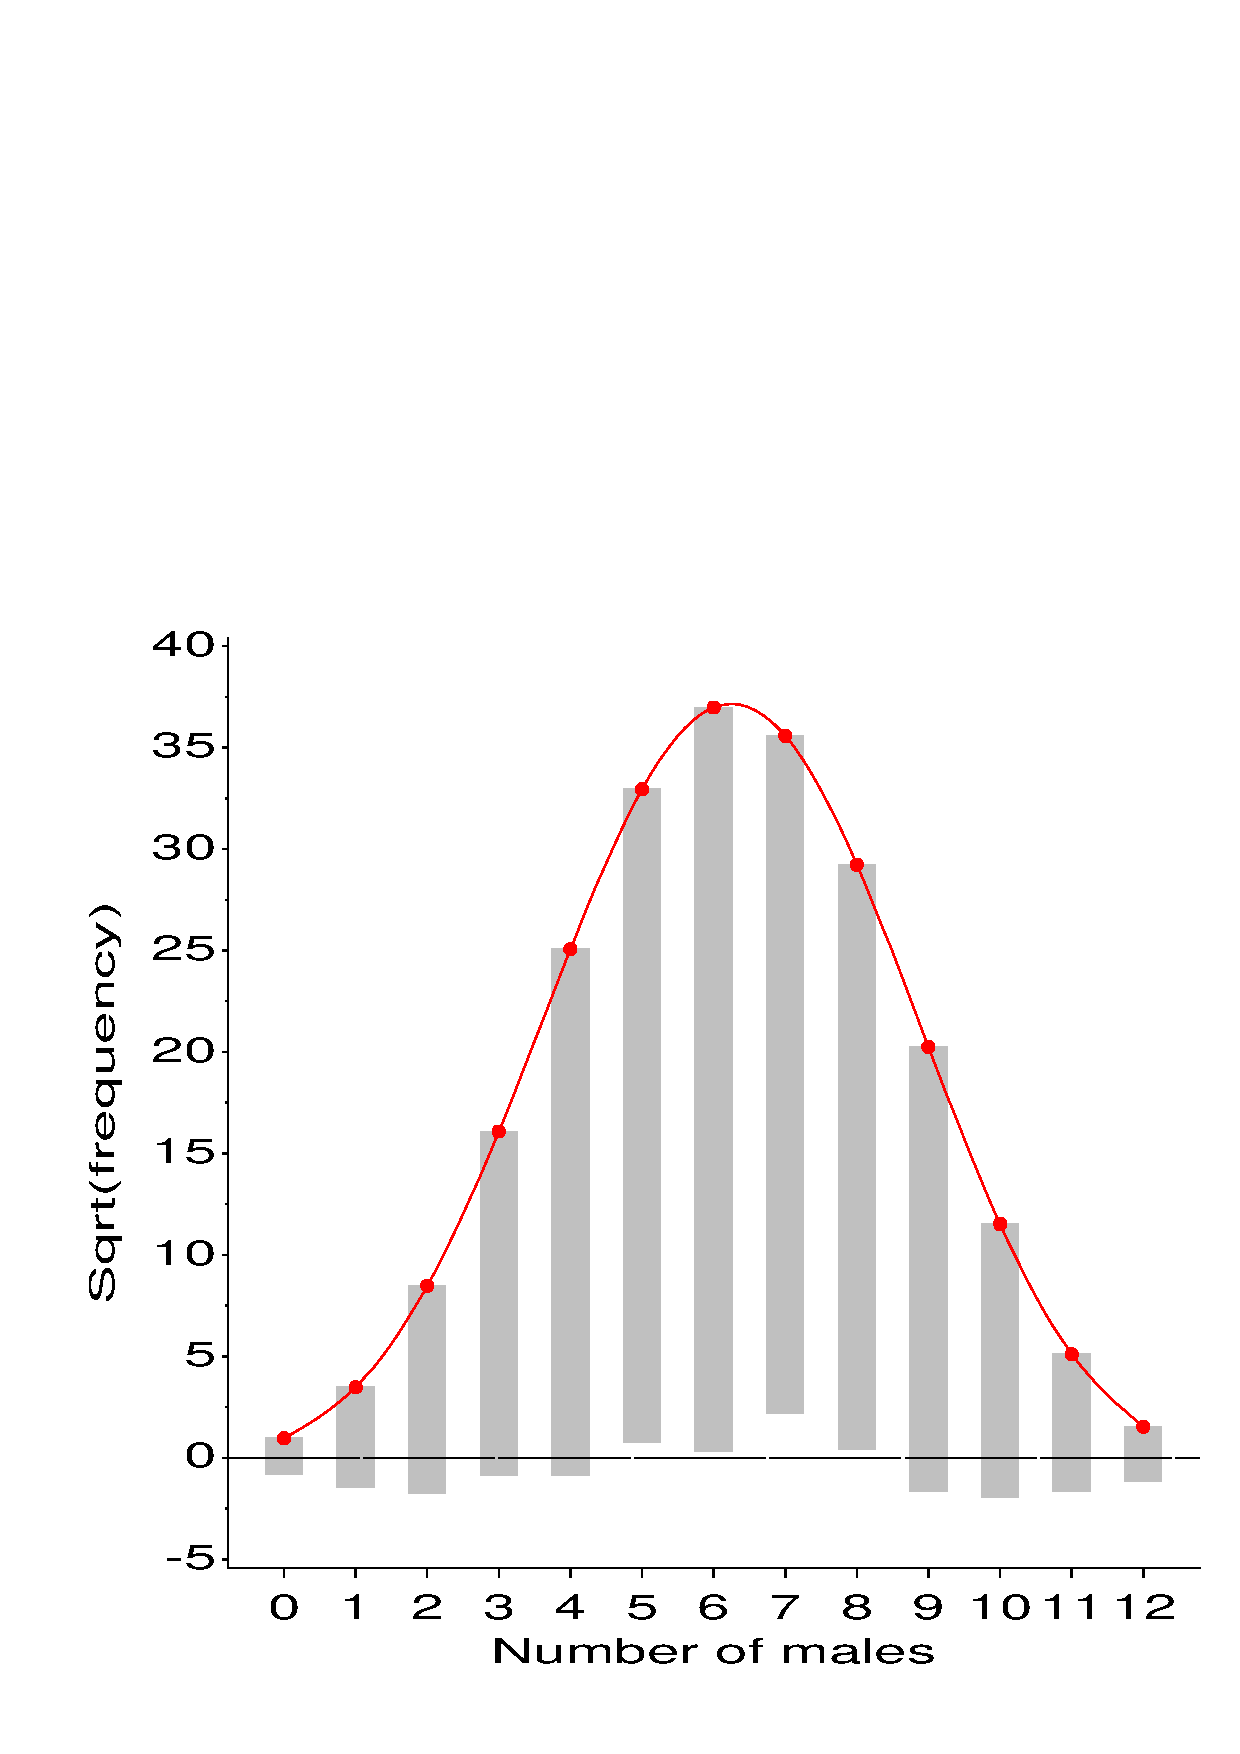
\includegraphics[width=1\linewidth]{saxony}\graphicsfile{ch2/fig/saxony.eps}{}
 \end{minipage}%
 \hfill
 \begin{minipage}[c]{.33\linewidth}
  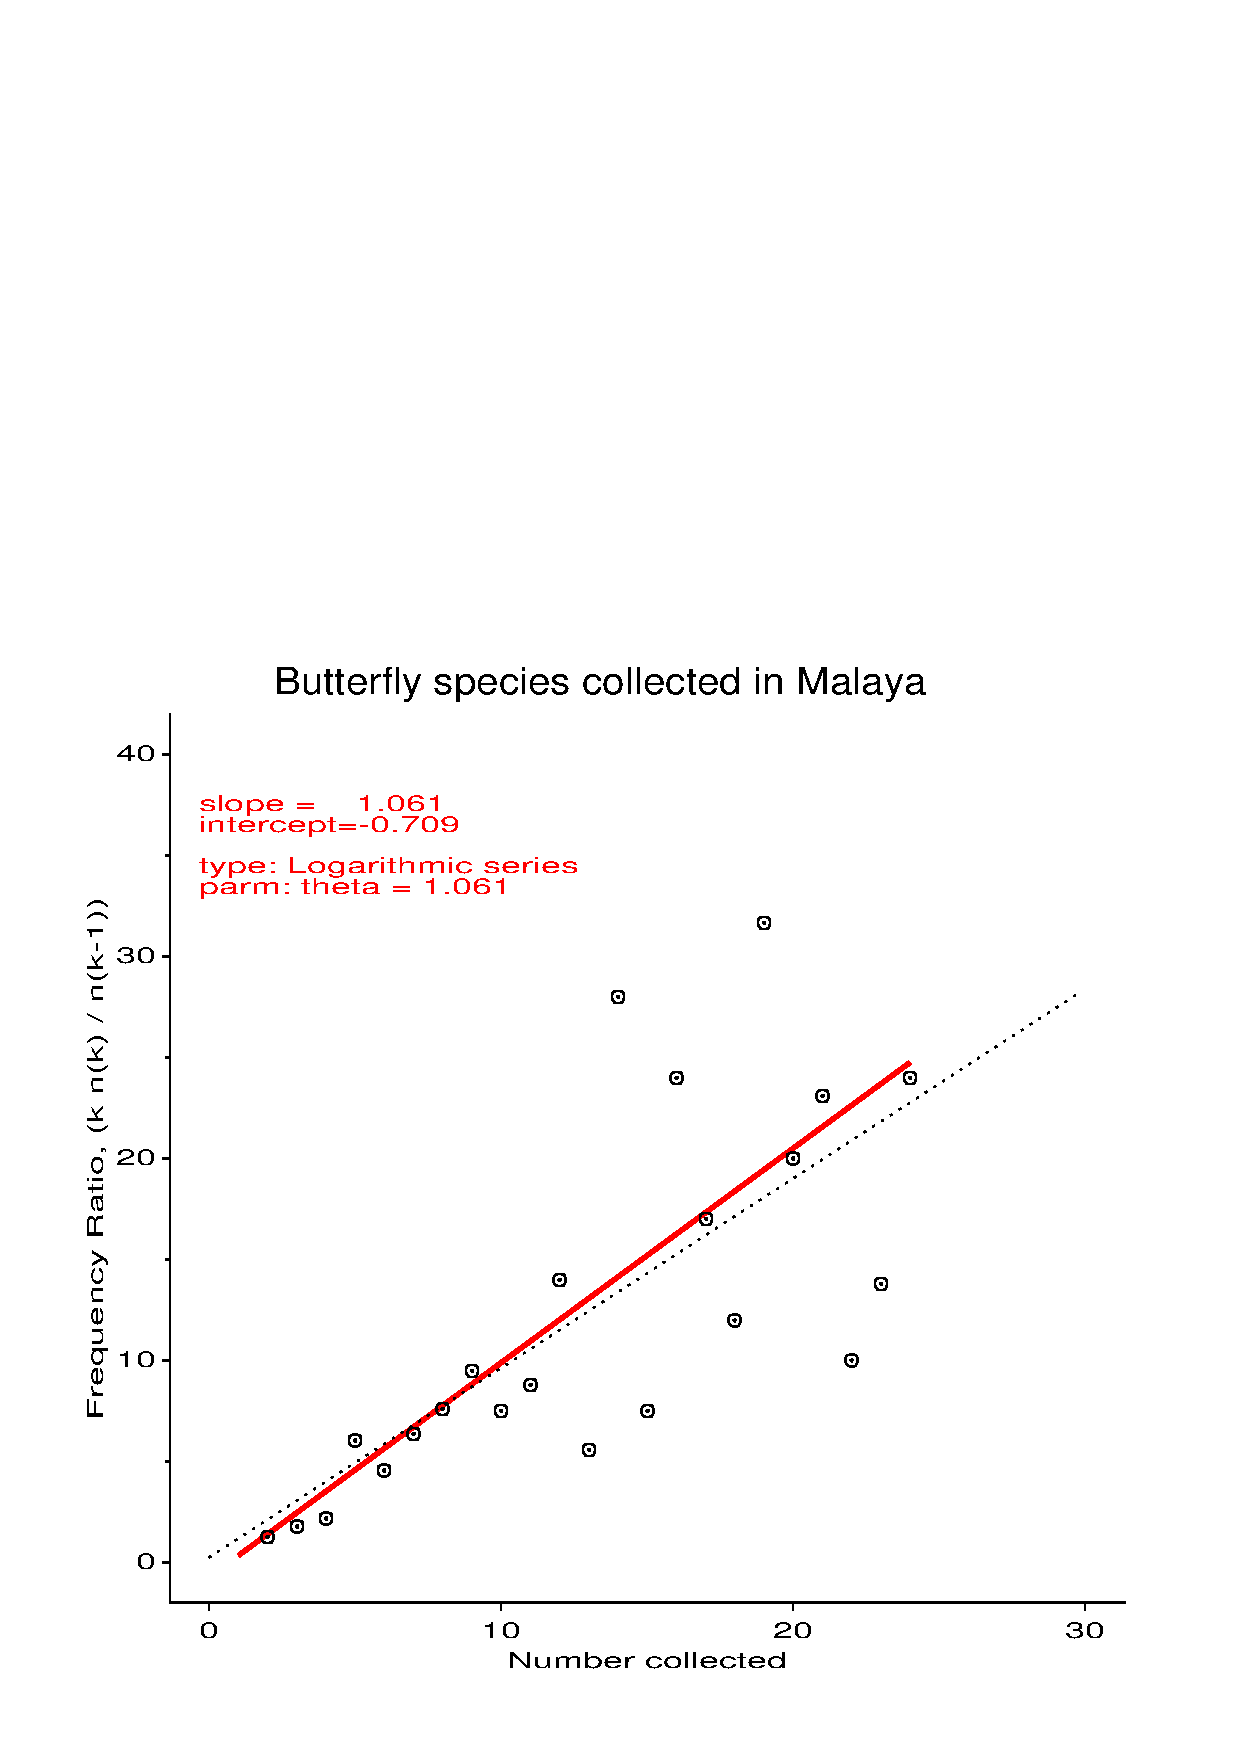
\includegraphics[width=1\linewidth]{orddemo3}\graphicsfile{ch2/fig/orddemo3.eps}{}
 \end{minipage}
 \hfill
 \begin{minipage}[c]{.33\linewidth}
  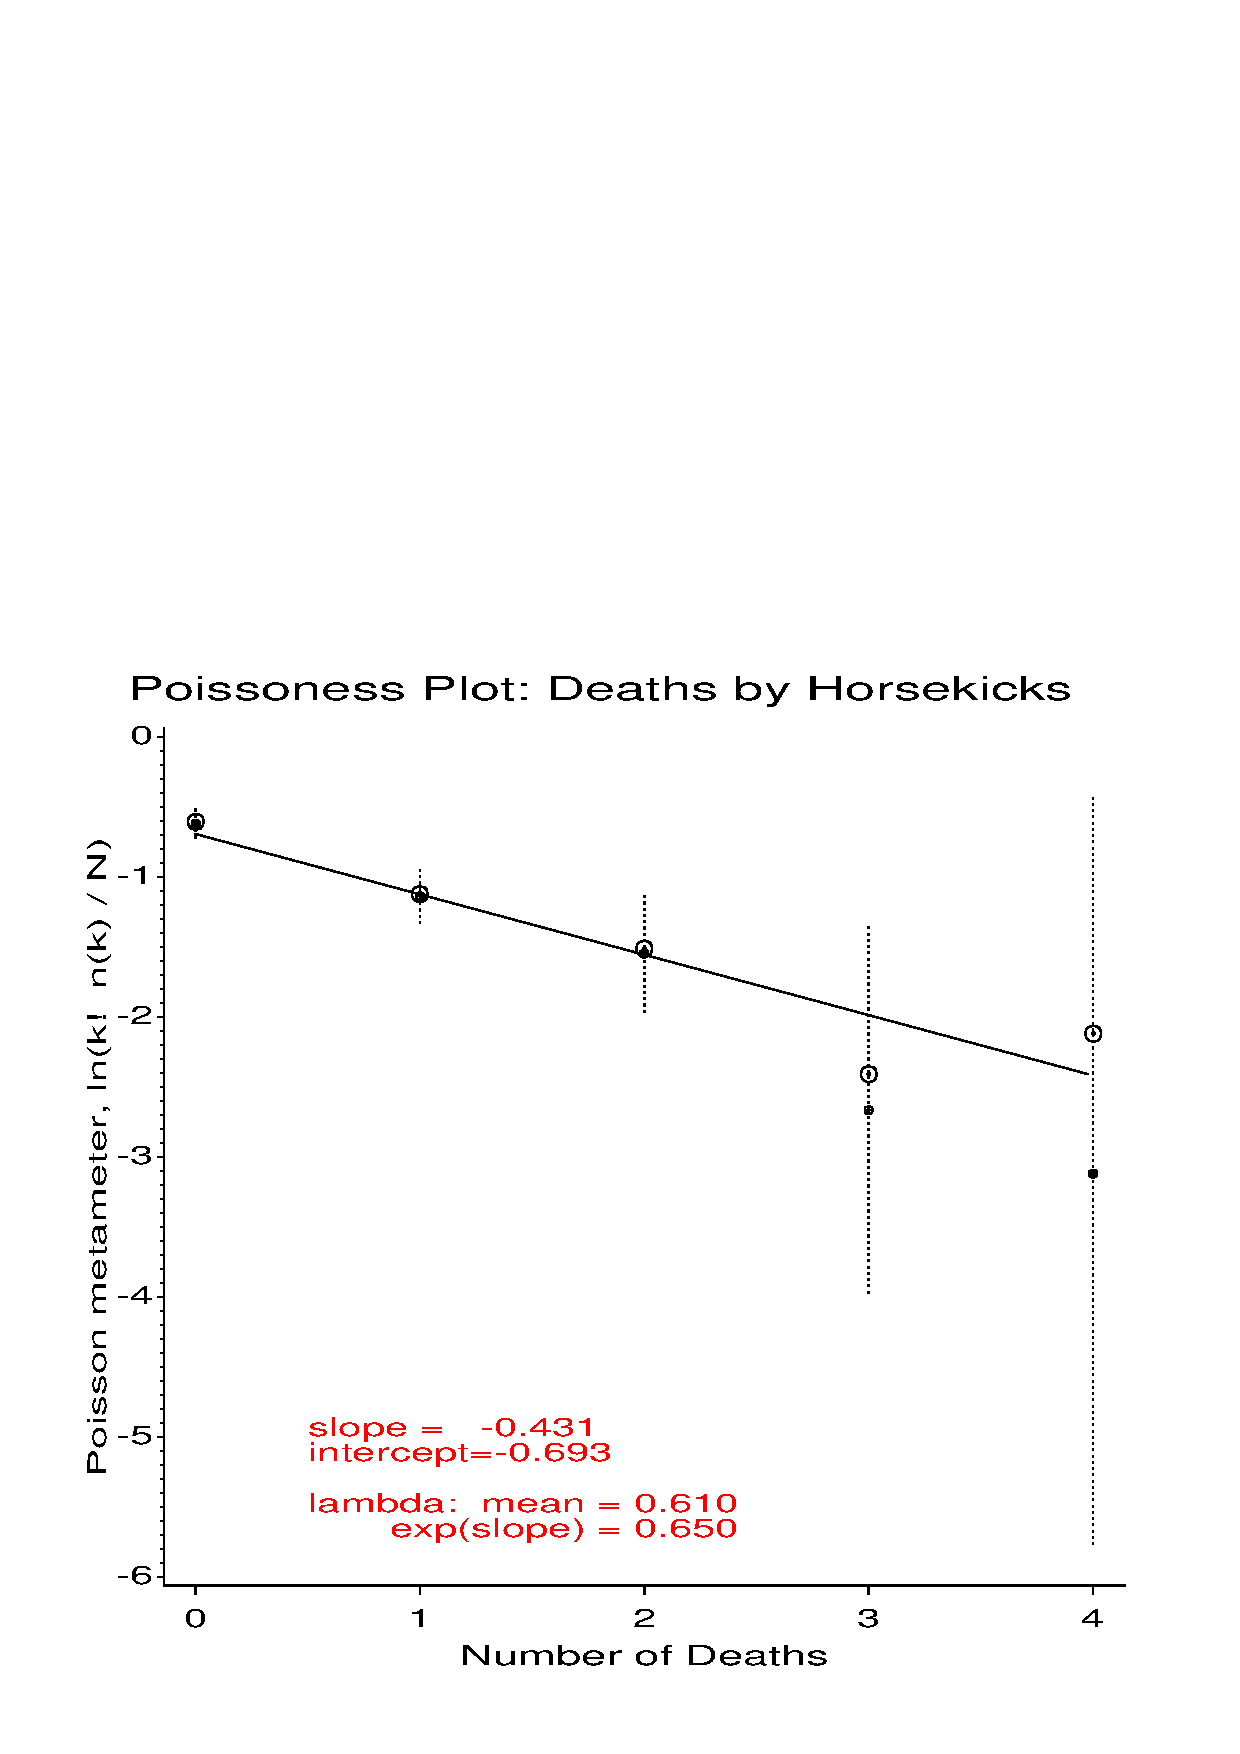
\includegraphics[width=1\linewidth]{poisdemo1}\graphicsfile{ch2/fig/poisdemo1.eps}{}
 \end{minipage}
\end{center}

		% visual table of contents

\chapterprelude{
Generalized linear models extend the familiar linear models of
regression and ANOVA to
include counted data, frequencies, and other data for which the
assumptions of independent, normal errors are not reasonable.
We rely on the analogies between ordinary and generalized linear
models (GLMs) to develop visualization methods to explore the data,
display the fitted relationships and check model assumptions.
The main focus of this chapter is on models for count data.
}
% \minitoc
% \clearpage

\epigraph{In one word, to draw the rule from experience, one must generalize; this is a necessity that imposes itself on the most circumspect observer.}
{Henri Poincar\'e, \emph{The Value of Science: Essential Writings of Henri Poincare}}

In the modern history of statistics, most developments occur incrementally, with
small additions to existing models and theory that extend their range
and applicability to new problems and data.  Occasionally, there is
a major synthesis that unites a wide class of existing methods in a
general framework and provides opportunities for far greater growth.

A prime example is the theory of generalized linear models, introduced
originally by \citet{NelderWedderburn:72}, that extended the familiar
(classical) linear models for regression and ANOVA to include related
models, such as logistic regression and logit models (described in \chref{ch:logistic})
and \loglin models (described in \chref{ch:loglin})
and other variations as ``families'' within a single general system.

This approach has proved attractive because it:
\begin{seriate}
 \item integrates many familiar statistical models in a general theory where they are
 just special cases;
 \item provides the basis for extending these and developing new models within the
 same or similar framework;
 \item simplifies the implementation of these models in software, since the same
 algorithm can be used for estimation, inference and assessing model adequacy
 for all generalized linear models.
\end{seriate}

\secref{glm:components} gives a brief sketch of the GLM framework.
The focus of this book is on visualization methods for categorical
data, and the two important topics concern models and methods for binomial response data
and for count data.  The first of these,
was described extensively in
\chref{ch:logistic},
with extensions to multinomial
data (\secref{sec:logist-poly})
% and multivariate responses
and there is little to add here, except for changes
in notation.

GLM models for count data, however, provide the opportunity to extend
the scope of these methods beyond what was covered in \chref{ch:loglin},
and this topic is introduced in \secref{sec:glm-count}.
The GLM framework also provides the opportunity to deal with common problems
of overdispersion (\secref{sec:glm-overdisp}) and an overabundance of
zero counts (\secref{sec:glm-overdisp}), giving some new models and
visualization methods that help to understand such data in greater detail.
\secref{sec:glm-diag} illustrates other graphical methods for diagnostic
model checking, some of which were introduced in earlier chapters.
Finally, \secref{sec:glm-multiv} outlines some simple extensions of these
models to handle multivariate responses.


\section{Components of Generalized Linear Models}\label{glm:components}

The motivation for the \term{generalized linear model} (GLM) and its structure are most
easily seen by considering the classical linear model,
\begin{equation*}
y_i = \vec{x}_i\trans \vec{\beta} + \epsilon_i
\end{equation*}
where
$y_i$ is the response variable for case $i, i=1, \dots n$,
$\vec{x}_i$ is the vector of explanatory variables or regressors,
$\vec{\beta}$ is the vector of model parameters, and the
$\epsilon_i$ are random errors.
In the classical linear model, the $\epsilon_i$ are assumed to
\begin{seriate}
  \item have constant variance, $\sigma^2_\epsilon$,
  \item follow a normal (Gaussian) distribution (conditional on $\vec{x}_i$),
  \item be independent across observations.
\end{seriate}

Thus, \citet{NelderWedderburn:72} generalized this Gaussian linear model to
consist of the following three components, by relaxing assumptions (a) and (b) above:%
\footnote{The remaining assumption of independent observations is relaxed in
\term{generalized linear mixed models} (GLMMs), in which random effects to account for non-independence
are added to the linear predictor.
This allows the modeling of correlated (responses of family members), clustered (residents in
different communities)
or hierarchical data
(patients within hospitals within regions). See: \citet{McCullochNeuhaus:2005} ...
\TODO{other references?}
}

\begin{description}
  \item[random component] The conditional distribution of the $y_i \given \vec{x}_i$,
  with mean $\E (y_i) = \mu_i$. Under classical assumptions,
  this is independent, normal with constant variance $\sigma^2$, i.e.,
  $ y_i \stackrel{\textrm{iid}}{\sim} N (\mu_i, \sigma^2)$.
  In the GLM, the probability distribution of the $y_i$ can be any member of the
  \term{exponential family}, including the normal, Poisson, binomial, gamma
  and others. Subsequent work has extended this framework to include
  multinomial distributions and some non-exponential families such as the
  negative binomial distribution.


  \item[systematic component] The idea that the predicted value of $y_i$ itself
  is a linear
  combination of the regressors is replaced by that of a \term{linear predictor},
  $\eta$, that captures this aspect of linear models,
\begin{equation*}
\eta_i = \vec{x}_i\trans \vec{\beta}
\end{equation*}


  \item[link function] The connection between the mean of the response, $\mu_i$,
  and the linear predictor, $\eta_i$, is specified by the \term{link function},
  $g(\bullet)$, giving
\begin{equation*}
g(\mu_i) = \eta_i = \vec{x}_i\trans \vec{\beta}
\end{equation*}
  The link function $g(\bullet)$ must be both \emph{smooth} and \emph{monotonic}, meaning that
  it is one-to-one, so an inverse transformation, $g^{-1}(\bullet)$ exists,
\begin{equation*}
\mu_i = g^{-1}(\eta_i) = g^{-1}(\vec{x}_i\trans \vec{\beta})
\end{equation*}
  which allows us to obtain and plot the predicted values on their original scale.  The link function
  captures the familiar idea that linear models are often estimated with a transformation
  of the response, such as $\log(y_i)$ for a frequency variable or $\logit(y_i)$
  for a binomial variable.  The inverse function $g^{-1}(\bullet)$
  is also called the \term{mean function}.
\end{description}

\begin{table}[htb]
\centering
\caption{Common link functions and their inverses used in generalized linear models}\label{tab:link-funcs}
\medskip
\renewcommand{\arraystretch}{1.25}
\begin{tabular}{lll}
\hline
%\rowcolor[gray]{.85}
\tableheader
Link name      & Function: $\eta_i = g(\mu_i)$ & Inverse: $\mu_i=g^{-1}(\eta_i)$  \\ \hline
identity       & $\mu_i$                       & $\eta_i$                      \\
square-root    & $\sqrt{\mu_i}$                & $\eta_i^2$                    \\
log            & $\log_e(\mu_i)$               & $\exp(\eta_i)$                \\ 
inverse        & $\mu_i^{-1}$                  & $\eta_i^{-1}$                 \\
inverse-square & $\mu_i^{-2}$                  & $\eta_i^{-1/2}$               \\ 
\hline
logit          & $\log_e\frac{\mu_i}{1-\mu_i}$ & $\frac{1}{1+\exp(-\eta_i)}$   \\
probit         & $\Phi^{-1}(\mu_i)$            & $\Phi^{-1}(\eta_i)$           \\
log-log        & $-\log_e[-\log_e(\mu_i)]$     & $\exp[-\exp(-\eta_i)]$        \\
comp. log-log  & $\log_e[-\log_e(1-\mu_i)]$    & $1-\exp[-\exp(\eta_i)]$       \\  \hline
\end{tabular}
\end{table}

Some commonly used link functions are shown in \tabref{tab:link-funcs}.
Some of these link functions have restrictions on the range of $y_i$
to which they can be applied.  For example, the square-root and log links
apply only to non-negative and
positive values respectively.
The last four link functions in this
table are for binomial data, where $y_i$ represents the observed proportion
of successes in $n_i$ independent trials, and thus the mean $\mu_i$
represents the probability of success (symbolized by $\pi_i$ in \chref{ch:logistic}).
Binary data are the special case where $n_i=1$.

\subsection{Variance functions}
The GLM has the additional property that, for distributions in the exponential family,
the conditional variance of $y_i \given \eta_i$ is a known function, $\V (\mu_i)$
of the mean and possibly one other parameter called the \term{scale parameter} or
\term{dispersion parameter}, $\phi$. Some commonly used distributions in the
exponential family and their variance functions are shown in \tabref{tab:exp-families}.

% Please add the following required packages to your document preamble:
% \usepackage[table,xcdraw]{xcolor}
% If you use beamer only pass "xcolor=table" option, i.e. \documentclass[xcolor=table]{beamer}
\begin{table}[htb]
\centering
\caption{Common distributions in the exponential family used with generalized linear models and their canonical link and variance functions}
\label{tab:exp-families}
\medskip
\renewcommand{\arraystretch}{1.25}
\begin{tabular}{lllll}
\hline
%\rowcolor[gray]{.85}
\tableheader
Family           & Notation          & Canonical link         & Range of $y$          & Variance function, $\V(\mu \given \eta)$ \\
\hline
Gaussian         & $N(\mu,\sigma^2)$ & identity: $\mu$        & $(-\infty, +\infty)$   & $\phi$                       \\
Poisson          & $\Pois(\mu)$      & $\log_e(\mu)$          & $0, 1, \dots, \infty$  & $\mu$                        \\
Negative-Binomial & $\NBin(\mu,\theta)$   & $\log_e(\mu)$     & $0, 1, \dots, \infty$ & $\mu + \mu^2/\theta$          \\
Binomial         & $\Bin(n,\mu)/n$   & $\logit(\mu)$          & $\{0, 1, \dots, n\}/n$ & $\mu (1-\mu)/n$              \\
Gamma            & $G(\mu, \nu)$     & $\mu^{-1}$             & $(0, +\infty)$         & $\phi \mu^2$                 \\
Inverse-Gaussian & $IG(\mu, \nu)$    & $\mu^2$                & $(0, +\infty)$         & $\phi \mu^3$                 \\
\hline
\end{tabular}
\end{table}

\begin{itemize}
\item In the classical Gaussian linear model, the conditional variance is constant,
$\phi = \sigma^2_\epsilon$.

\item In the Poisson family, $\V (\mu_i) = \mu_i$
and the dispersion parameter is fixed at $\phi = 1$.
In practice, it is common for count data to exhibit \term{overdispersion},
meaning that $\V (\mu_i) > \mu_i$.  One way to correct for this is to extend
the GLM to allow the dispersion parameter to be estimated from the data,
giving what is called the \term{quasi-Poisson} family, with $\V (\mu_i) = \widehat{\phi} \mu_i$.

\item Similarly, for binomial data, the variance function is $\V (\mu_i) = \mu_i (1-\mu_i) / n_i$,
with $\phi$ fixed at 1.
Overdispersion often results from failures of the assumptions of the binomial model:
supposedly independent observations may be correlated or clustered and the probability
of success may not be constant, or vary with unmeasured or unmodeled variables.

\item The gamma and inverse-Gaussian families are distributions useful for modeling a continuous
and positive response variable with no upper bound (e.g., reaction time). They both have the
property that conditional variance increases with the mean, and for the inverse-Gaussian,
variance increases at a faster rate.  Their dispersion parameters $\phi$ are simple functions
of their intrinsic ``shape'' parameters, indicated as $\nu$ in the table.

\end{itemize}

The important points from this discussion are that the GLM together with the exponential
family of distributions:
\begin{itemize}
 \item provide for simple, linear relations between the response and the predictors
 via the link function and the linear predictor.
 \item allows a very flexible relationship between the mean and
 conditional variance to be specified in terms of a set of known families.
 \item incorporates a dispersion parameter $\phi$ that in some cases can be estimated
 or tested for departure from that entailed in a given family.
 \item has allowed further extensions of this framework outside the exponential family,
 ranging from simple adjustments for statistical inference (``quasi'' families,
 adjusted ``sandwich'' covariances) to separate modeling of the variance relation
 to the predictors.
\end{itemize}

Further details of generalized linear models are beyond the scope of this book, but
the interested reader should consult \citet[\S 15.3]{Fox:2008}
and \citet[Ch. 4]{Agresti:2013} for a comprehensive
treatment.

\subsection{Hypothesis tests for coefficients}\label{sec:glm-hyptests}
GLMs are fit using maximum likelihood estimation, and implemented in software using
an iterative algorithm known as \emph{iteratively weighted least squares}
that generalizes the least squares method for classical linear models.
This provides estimates $\vec{\widehat{\beta}}$ of the model coefficients
for the predictors in $\vec{x}$, as well as an estimated asymptotic
(large sample) variance matrix of $\vec{\widehat{\beta}}$, given by
\begin{equation}\label{eq:varbeta}
\V (\widehat{\vec{\beta}}) = \phi ( \mat{X}\trans  \mat{W} \mat{X} )
\end{equation}
where $\mat{W}$ is a diagonal matrix of weights computed in the final iteration.
In the standard Poisson GLM, the weight matrix is $\mat{W} = \diag (\widehat{\vec{\mu}})$
and $\phi=1$ is assumed.

Asymptotic standard errors, $ \mathrm{se} (\widehat{\beta}_j)$,
for the coefficients are then the square roots of the
diagonal elements
% $ \sqrt{ \V (\widehat{\vec{\beta}})_{jj}}$,
of $\V (\widehat{\vec{\beta}})$, and tests of hypotheses regarding
an individual coefficient, e.g., $H_0 : \beta_j = 0$, can be carried out
using the Wald test statistic,
$z_j = \widehat{\beta}_j / \mathrm{se} (\widehat{\beta}_j)$.
When the null hypothesis is true, $z_j$ has a standard normal $\mathcal{N}(0,1)$
distribution, providing $p$-values for significance tests.%
\footnote{Wald tests are sometimes carried out using $z^2$, which has an equivalent
$\chi^2_1$ distribution with 1 degree of freedom.
}

More generally, we can test any \term{linear hypothesis}, of the form
$H_0 : \mat{L} \vec{\beta} = \vec{c}$, where $\mat{L}$ is a constant hypothesis matrix
of size $h \times p$ giving $h$ linear combinations of the coefficients,
to be tested for equality with the constants in $\vec{c}$, typically taken as $\vec{c}=\vec{0}$.
The test statistic is the Wald chi-square,
\begin{equation}\label{eq:waldchisq}
Z^2 = (\mat{L} \widehat{\vec{\beta}} - \vec{c})\trans \:
      [\mat{L} \V (\widehat{\vec{\beta}}) \mat{L}\trans]^{-1} \:
      (\mat{L} \widehat{\vec{\beta}} - \vec{c})
\end{equation}
which has a $\chisq$ distribution on $h$ degrees of freedom.%
\footnote{When a dispersion parameter $\phi$ has been estimated from the data,
it is common to use an $F$-test, using the statistic $F = Z^2 / h$,
with $h$ and $n-p$ degrees of freedom.}

For example, to test the hypothesis
that all of
$\beta_1 = \beta_2 = \beta_3 =0$ in a model with three predictors, you can use
\begin{equation*}
\mat{L} = \left[
{\begin{array}{*{20}{c}}
0 & 1 & 0 & 0\\
0 & 0 & 1 & 0\\
0 & 0 & 0 &1
\end{array}}
\right] =
\left[
{\begin{array}{*{20}{c}}
{\vec{0}} & {\mat{I}}
\end{array}}
\right]
\comma
\quad\quad
\vec{c} = \left(
{\begin{array}{*{20}{c}}
0\\
0\\
0
\end{array}}
\right)
\end{equation*}
Similarly, to test the hypothesis that $\beta_1 = \beta_2$ in the same model,
you can use $\mat{L} = [0, 1, -1, 0]$ and $\vec{c} = [0]$.%
\footnote{Such a test is only sensible if the predictors $\vec{x_1}$ and $\vec{x_2}$
are on the same scale, so their coefficients are commensurable.}

In \R, such tests are most conveniently carried out using \func{linearHypothesis}
in the \Rpackage{car}.  The hypothesis matrix $\mat{L}$ can be supplied as a
numeric matrix, or more conveniently,
the hypothesis can be specified symbolically as a character vector
of the names of the coefficients involved in each row of $\mat{L}$.
For example, the first hypothesis test above could be specified using the vector
\code{c("x1=0", "x2=0", "x3=0")} and the test of equality as
\code{"x1-x2=0"}.

\subsection{Goodness-of-fit tests}\label{sec:glm-goodfit}
The basic ideas for testing goodness-of-fit were discussed in \secref{sec:loglin-goodfit}
in connection with \loglin models for \ctabs.
As before, these assess the overall performance of a model in reproducing the data.
The commonly used measures include the Pearson chi-square and
\LR deviance statistics, which can be seen as weighted sums of residuals.
We re-state these test statistics here in the wider context of the GLM.

Let $y_i, i=1, 2, \dots, n$ be the response and $\widehat{\mu}_i = g^{-1} (\vec{x}_i\trans \widehat{\vec{\beta}})$
the fitted mean using the estimated coefficients, having estimated variance
$\widehat{\omega}_i = \V(\widehat{\mu}_i\given \eta_i)$ as in \tabref{tab:exp-families}.
Then the normalized squared residual for observation $i$ is
$(y_i - \widehat{\mu}_i)^2 / \widehat{\omega}_i$, and the Pearson statistic is
\begin{equation}\label{eq:pearson}
X^2_P = \sum_{i=1}^n \frac{(y_i - \widehat{\mu}_i)^2}{\widehat{\omega}_i} \period
\end{equation}

In the GLM for count data, the main focus of this chapter, the Poisson family
sets $\omega = \mu$ with the dispersion parameter fixed at $\phi=1$.

The \term{residual deviance} statistic, as in logistic regression and \loglin models
is defined as twice the difference between the maximum possible log-likelihood
for the \emph{saturated model} that fits perfectly and maximized log-likelihood
for the fitted model. The deviance can be defined as
\begin{equation*}
D (\vec{y}, \vec{\widehat{\mu}}) \equiv 2 [ \log_e \mathcal{L}(\vec{y};\vec{y}) - \log_e \mathcal{L}(\vec{y};\vec{\widehat{\mu}})]
\end{equation*}
For classical linear models under normality, the deviance is simply the residual sum of squares,
$\sum_i^n (y_i - \widehat{\mu}_i)$.  This has led to the deviance being taken in the GLM
framework as a generalization of the sum of squares used in ANOVA, and hence, an analogous
\term{analysis of deviance} to carry out tests for individual terms in GLMs, or to compare
nested models.

In \R, \code{anova(mod)} for the \class{glm} object \code{mod}
gives \emph{sequential} (``Type I'') tests of successive terms in a model, while
\func{Anova} in the \Rpackage{car} gives the more generally useful
``Type II'' (and ``Type III'') \emph{partial} tests, that assess the additional
contribution of each term above all others, taking marginality into account.

For Poisson models with a log link giving $\vec{\mu} = \exp(\vec{x}\trans \vec{\beta})$ , the deviance takes the form%
\footnote{In the context of the \loglin models discussed in \secref{sec:loglin-goodfit}, this is also referred to
as the \LR $G^2$ statistic.}

\begin{equation}\label{eq:pois-deviance}
D (\vec{y}, \vec{\widehat{\mu}}) =
  2 \sum_{i=1}^n \left[ y_i \log_e \left( \frac{y_i}{\widehat{\mu}_i} \right) - (y_i - \widehat{\mu}_i) \right]
\end{equation}
For a GLM with $p$ parameters, both the Pearson and residual deviance statistics follow
approximate $\chi^2_{n-p}$ distributions with $n-p$ degrees of freedom.

% \section{GLMs for binomial data}\label{sec:glm-binomial}
%
% \TODO{Don't need to include this, because these models were extensively treated in \chref{ch:logistic}.}

\subsection{Comparing non-nested models}\label{sec:glm-nonnest}

The flexibility of the GLM and its extensions allows us to fit models
to the same data using different families and different link functions, and to
fit models that allow for overdispersion (\secref{sec:glm-overdisp})
or that make special provisions for zero counts (\secref{sec:glm-zeros}).
One price paid for this additional versatility is that standard
LR tests and $F$ tests (such as provided by \func{anova}
and \func{linearHypothesis} in the \Rpackage{car})
do not apply to models that are not nested, that is, where one
model cannot be represented as a restricted, special case of another.

For models estimated by maximum likelihood, one general route to comparing
non-nested models is through the AIC information criterion proposed initially
by \citet{Akaike:73} and the related BIC criterion \citep{Schwartz:78}
based on the fitted log-likelihood function.
\begin{eqnarray}
\textrm{AIC} & = & -2 \log_e \mathcal{L} + 2 k \\
\textrm{BIC} & = & -2 \log_e \mathcal{L} + \log_e(n) k
\end{eqnarray}
As noted in \secref{sec:loglin-goodfit}, these both penalize models with larger $k$,
the number of parameters in the model, with BIC adding a greater penalty with
larger sample size.
However, because they are based only on the
maximized log-likelihood, they are agnostic as to whether models are nested or not,
and give comparable results (lower is better) provided the same observations have
been used in all models.

In \R, these results are given for a collection of models by the generic functions
\func{AIC} and \func{BIC}; these can be calculated for any model for which
\func{logLik} and (for BIC) \func{nobs} methods exist.
The \pkg{vcdExtra} function \func{Summarise} is a convenient wrapper for these
methods.

AIC and BIC do not give significance tests for assessing whether one model is
significantly ``better'' than another.  One test that \emph{does} this was proposed by
\citet{Vuong:1989}, unsurprisingly called \term{Vuong's test}.
The test is based on comparing the predicted probabilities
or the pointwise log-likelihoods of the two models, and tests the null hypothesis
that each is equally close to the saturated model, against the alternative that
one model is closer.

For two such models, let $f_1 (y_i \given \vec{x}_i, \vec{\theta}_1)$
be the density function under model 1, with parameters $\vec{\theta}_1$
and similarly
$f_2 (y_i \given \vec{x}_i, \vec{\theta}_2)$ under model 2 with parameters $\vec{\theta}_2$,
where $f_1(\bullet)$ and $f_2(\bullet)$ need not be the same.
Vuong's test compares these based on the observation-wise log-likelihood ratios,
%\newcommand{\ell}{\mathcal{l}}
\begin{equation*}
\ell_i = \log_e \left(
              \frac{f_1 (y_i \given \vec{x}_i, \vec{\widehat{\theta}}_1)}
                   {f_2 (y_i \given \vec{x}_i, \vec{\widehat{\theta}}_2)} \right)
\end{equation*}
The test statistic is
\begin{equation*}
 V = \frac{\bar{\ell} - \textrm{penalty}} {\sqrt{n} s_\ell}
\end{equation*}
where $\bar{\ell}$ is the mean of the $\ell_i$, $s_\ell$ is their variance, and
penalty is an adjustment for model parsimony, typically taken as
$\log(n) (k_1 - k_2)/2$ when model 1 has $k_1$ parameters in $\vec{\theta}_1$
and model 2 has $k_2$ parameters in $\vec{\theta}_2$.

The test statistic $V$ has an asymptotic normal $N(0,1)$ distribution,
and is directional, with large positive values favoring model 1, and large
negative values favoring model 2.
This test is implemented as the \func{vuong} function in the \Rpackage{pscl}.

\section{GLMs for count data}\label{sec:glm-count}

%\section{GLMs for count data}\label{sec:glm-count}

The prototypical GLM for count data, where the response $y_i$
takes on non-negative values $0, 1, 2, \dots$,
uses the Poisson family with the log link.
We used this model extensively throughout all of \chref{ch:loglin}.
There the focus was on the special case of the \loglin model
applied largely to contingency tables, where the \loglin model could
be seen as a fairly direct extension of ANOVA models for a
quantitative response applied to the log of cell frequency.

The advantage there was that models for two-way, three-way and
by implication \nway tables could be discussed and illustrated
using notation and graphs that separated the parameters and
effects for one-way terms (``main effects''), two-way terms
(``simple associations'') and higher-way terms (``conditional associations'').

The disadvantage is that these models as formulated there do not
easily accommodate general quantitative predictors and
were limited to the log link and the Poisson family.
For example, the models discussed in \secref{sec:loglin-ordinal}
for ordinal variables allow one or more table factors to be
assigned quantitative scores or have such scores estimated from
the data, as in RC() models (\secref{sec:RCmodels}).
Yet, the \ctab approach for \loglin models breaks down if there are
continuous predictors, and count data often exhibits features that
make the equivalent Poisson regression model unsuitable or incomplete.
We consider some extended models here.


\begin{Example}[phdpubs1]{Publications of PhD candidates}
In \exref{ex:phdpubs0} we considered the distribution of the number of
publications by PhD candidates in their last three years of study,
but without taking any available predictors into account.
For these data, a simple calculation shows why the Poisson distribution
is unsuitable (for the marginal distribution), because the variance is 2.19 times the mean.

\begin{knitrout}
\definecolor{shadecolor}{rgb}{1, 0.961, 0.933}\color{fgcolor}\begin{kframe}
\begin{alltt}
\hlkwd{data}\hlstd{(}\hlstr{"PhdPubs"}\hlstd{,} \hlkwc{package}\hlstd{=}\hlstr{"vcdExtra"}\hlstd{)}
\hlkwd{with}\hlstd{(PhdPubs,} \hlkwd{c}\hlstd{(}\hlkwc{mean}\hlstd{=}\hlkwd{mean}\hlstd{(articles),} \hlkwc{var}\hlstd{=}\hlkwd{var}\hlstd{(articles),}
                \hlkwc{ratio}\hlstd{=}\hlkwd{var}\hlstd{(articles)}\hlopt{/}\hlkwd{mean}\hlstd{(articles)))}
\end{alltt}
\begin{verbatim}
##   mean    var  ratio 
## 1.6929 3.7097 2.1914
\end{verbatim}
\end{kframe}
\end{knitrout}
The earlier example showed rootograms (in \figref{fig:phdpubs-rootogram})
of the number of articles, but here it is useful to consider some more
basic exploratory displays.  A basic barplot of the frequency distribution
of number of articles published is shown in the left panel of
\figref{fig:phdpubs-barplot}.  A quick look indicates that the distribution
is highly skewed and there is a large number of counts of zero.

Another problem is that the frequencies of 0--2 articles account for
over 75\% of the total, so that the frequencies of the larger counts
get lost in the display.  The rootogram corrects for this by plotting
frequency on the square-root scale.  However, because we are contemplating
a model with a log link, the same goal can be achieved by plotting
log of frequency, as shown in the right panel of \figref{fig:phdpubs-barplot}.
To accommodate the zero frequencies, the plot shows log(Frequency+1),
avoiding errors from \code{log(0)}.
It can be seen that log frequency decreases steadily up to 7 articles and
then levels off approximately.

\begin{figure}[htb]
  \centering
  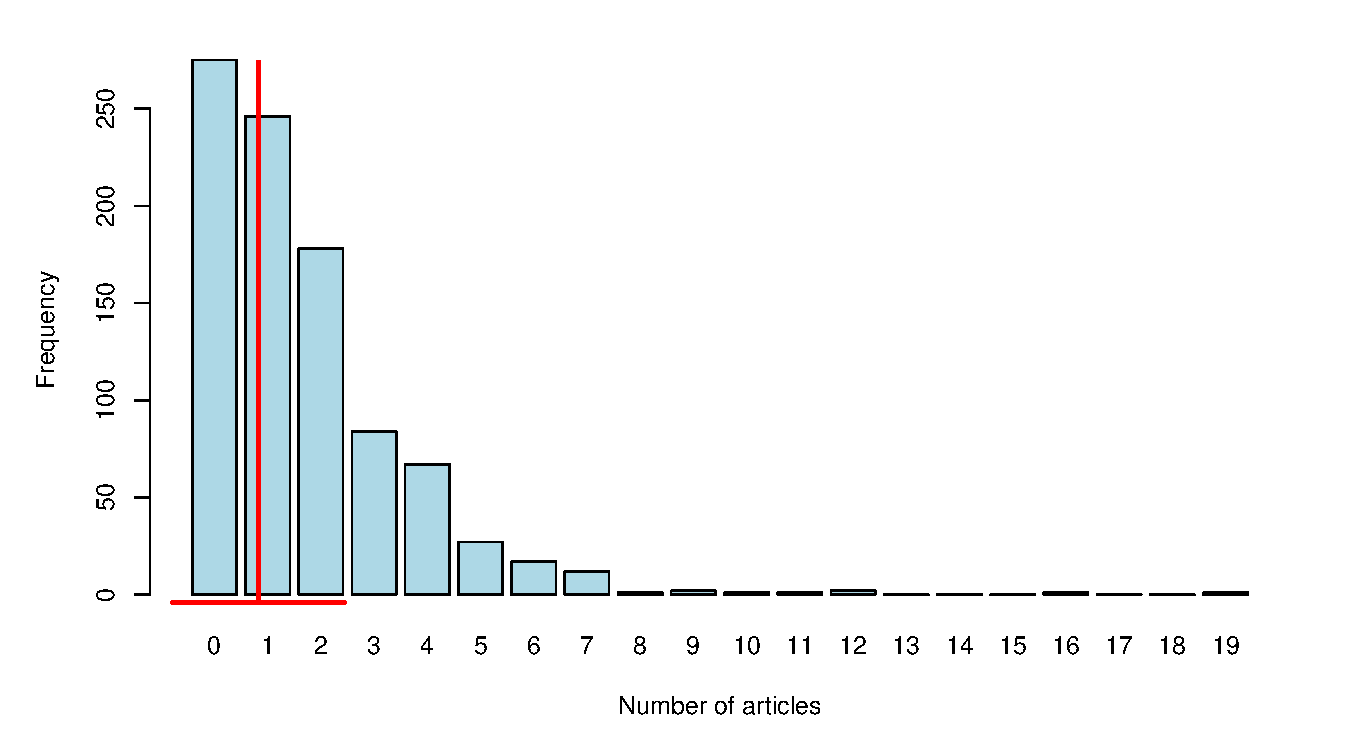
\includegraphics[width=.49\textwidth]{ch09/fig/phdpubs-barplot1}
  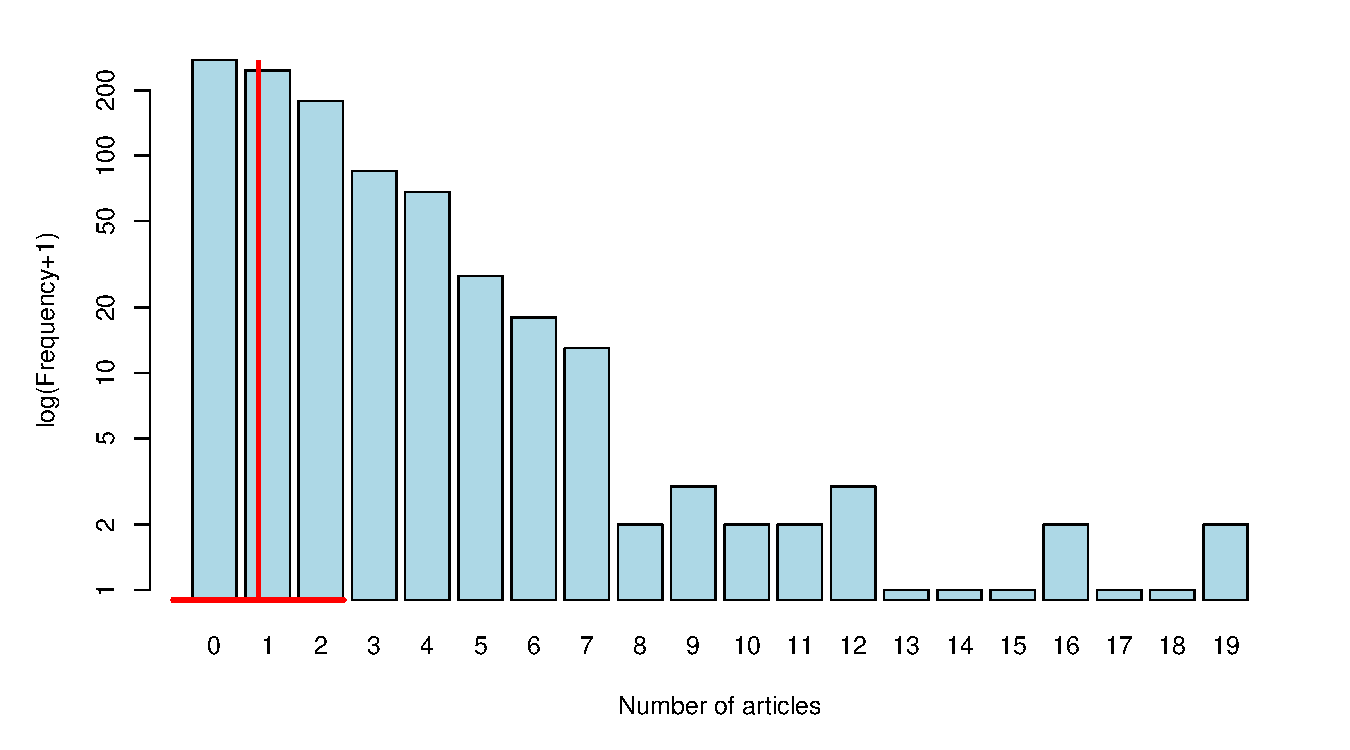
\includegraphics[width=.49\textwidth]{ch09/fig/phdpubs-barplot2}
  \caption{Barplots showing the frequency distribution of number of publications by PhD candidates.
  Left: raw scale; Right: a log scale makes the smaller counts more visible. The vertical red
  lines show the mean and horizontal lines show mean $\pm 1$  standard deviation.}
  \label{fig:phdpubs-barplot}
\end{figure}

These plots are produced as shown below.  The frequency distribution of
\code{articles} can be tabulated by \func{table}, but there is a subtle
wrinkle here:  By default, \func{table} excludes the values of \code{articles}
that do not occur in the data (zero frequencies).  To include all values in
the entire range, it is necessary to treat \code{articles} as a factor
with levels \code{0:19}.

\begin{knitrout}\footnotesize
\definecolor{shadecolor}{rgb}{1, 0.961, 0.933}\color{fgcolor}\begin{kframe}
\begin{alltt}
\hlstd{art.fac} \hlkwb{<-} \hlkwd{factor}\hlstd{(PhdPubs}\hlopt{$}\hlstd{articles,} \hlkwc{levels}\hlstd{=}\hlnum{0}\hlopt{:}\hlnum{19}\hlstd{)}  \hlcom{# include zero frequencies}
\hlstd{art.tab} \hlkwb{<-} \hlkwd{table}\hlstd{(art.fac)}
\hlstd{art.tab}
\end{alltt}
\begin{verbatim}
## art.fac
##   0   1   2   3   4   5   6   7   8   9  10  11  12  13  14  15  16  17  18  19 
## 275 246 178  84  67  27  17  12   1   2   1   1   2   0   0   0   1   0   0   1
\end{verbatim}
\end{kframe}
\end{knitrout}
Then, the basic plot on the frequency scale is created using \func{barplot},
and some annotations showing the mean and a one standard deviation interval
can be added using standard plotting tools.
\begin{knitrout}
\definecolor{shadecolor}{rgb}{1, 0.961, 0.933}\color{fgcolor}\begin{kframe}
\begin{alltt}
\hlkwd{barplot}\hlstd{(art.tab,} \hlkwc{xlab}\hlstd{=}\hlstr{"Number of articles"}\hlstd{,} \hlkwc{ylab}\hlstd{=}\hlstr{"Frequency"}\hlstd{,}
        \hlkwc{col}\hlstd{=}\hlstr{"lightblue"}\hlstd{)}
\hlkwd{abline}\hlstd{(}\hlkwc{v}\hlstd{=}\hlkwd{mean}\hlstd{(PhdPubs}\hlopt{$}\hlstd{articles),} \hlkwc{col}\hlstd{=}\hlstr{"red"}\hlstd{,} \hlkwc{lwd}\hlstd{=}\hlnum{3}\hlstd{)}
\hlstd{ci} \hlkwb{<-} \hlkwd{mean}\hlstd{(PhdPubs}\hlopt{$}\hlstd{articles)}\hlopt{+}\hlkwd{c}\hlstd{(}\hlopt{-}\hlnum{1}\hlstd{,}\hlnum{1}\hlstd{)} \hlopt{*} \hlkwd{sqrt}\hlstd{(}\hlkwd{var}\hlstd{(PhdPubs}\hlopt{$}\hlstd{articles))}
\hlkwd{lines}\hlstd{(}\hlkwc{x}\hlstd{=ci,} \hlkwc{y}\hlstd{=}\hlkwd{c}\hlstd{(}\hlopt{-}\hlnum{4}\hlstd{,} \hlopt{-}\hlnum{4}\hlstd{),} \hlkwc{col}\hlstd{=}\hlstr{"red"}\hlstd{,} \hlkwc{lwd}\hlstd{=}\hlnum{3}\hlstd{,} \hlkwc{xpd}\hlstd{=}\hlnum{TRUE}\hlstd{)}
\end{alltt}
\end{kframe}
\end{knitrout}

Similarly, the plot on the log scale in the right panel of \figref{fig:phdpubs-barplot}
is produced with \func{barplot}, but using \code{art.tab+1} to start frequency at one
and \code{log="y"} to scale the vertical axis to log.

\begin{knitrout}
\definecolor{shadecolor}{rgb}{1, 0.961, 0.933}\color{fgcolor}\begin{kframe}
\begin{alltt}
\hlkwd{barplot}\hlstd{(art.tab}\hlopt{+}\hlnum{1}\hlstd{,} \hlkwc{ylab}\hlstd{=}\hlstr{"log(Frequency+1)"}\hlstd{,} \hlkwc{xlab}\hlstd{=}\hlstr{"Number of articles"}\hlstd{,}
        \hlkwc{col}\hlstd{=}\hlstr{"lightblue"}\hlstd{,} \hlkwc{log}\hlstd{=}\hlstr{"y"}\hlstd{)}
\end{alltt}
\end{kframe}
\end{knitrout}
Other useful exploratory plots for count data include boxplots of the response (on a log scale)
and scatterplots against continuous predictors, where jittering the response is often
necessary to avoid overplotting and a smooth nonparametric curve can show possible non-linearity.
The \code{log="y"} option is again handy, and the formula
method allows adding a start value to the response.  \figref{fig:phdpubs-logplots}
illustrates these ideas, for the factor \code{married} and the covariate \code{mentor}.
\begin{knitrout}
\definecolor{shadecolor}{rgb}{1, 0.961, 0.933}\color{fgcolor}\begin{kframe}
\begin{alltt}
\hlkwd{boxplot}\hlstd{(articles}\hlopt{+}\hlnum{1} \hlopt{~} \hlstd{married,} \hlkwc{data}\hlstd{=PhdPubs,} \hlkwc{log}\hlstd{=}\hlstr{"y"}\hlstd{,} \hlkwc{varwidth}\hlstd{=}\hlnum{TRUE}\hlstd{,}
        \hlkwc{ylab}\hlstd{=}\hlstr{"log(articles+1)"}\hlstd{,} \hlkwc{xlab}\hlstd{=}\hlstr{"married"}\hlstd{,} \hlkwc{cex.lab}\hlstd{=}\hlnum{1.25}\hlstd{)}
\hlkwd{plot}\hlstd{(}\hlkwd{jitter}\hlstd{(articles}\hlopt{+}\hlnum{1}\hlstd{)} \hlopt{~} \hlstd{mentor,} \hlkwc{data}\hlstd{=PhdPubs,} \hlkwc{log}\hlstd{=}\hlstr{"y"}\hlstd{,}
      \hlkwc{ylab}\hlstd{=}\hlstr{"log(articles+1)"}\hlstd{,} \hlkwc{cex.lab}\hlstd{=}\hlnum{1.25}\hlstd{)}
\hlkwd{lines}\hlstd{(}\hlkwd{lowess}\hlstd{(PhdPubs}\hlopt{$}\hlstd{mentor, PhdPubs}\hlopt{$}\hlstd{articles}\hlopt{+}\hlnum{1}\hlstd{),} \hlkwc{col}\hlstd{=}\hlstr{"blue"}\hlstd{,} \hlkwc{lwd}\hlstd{=}\hlnum{3}\hlstd{)}
\end{alltt}
\end{kframe}\begin{figure}[!htbp]


\centerline{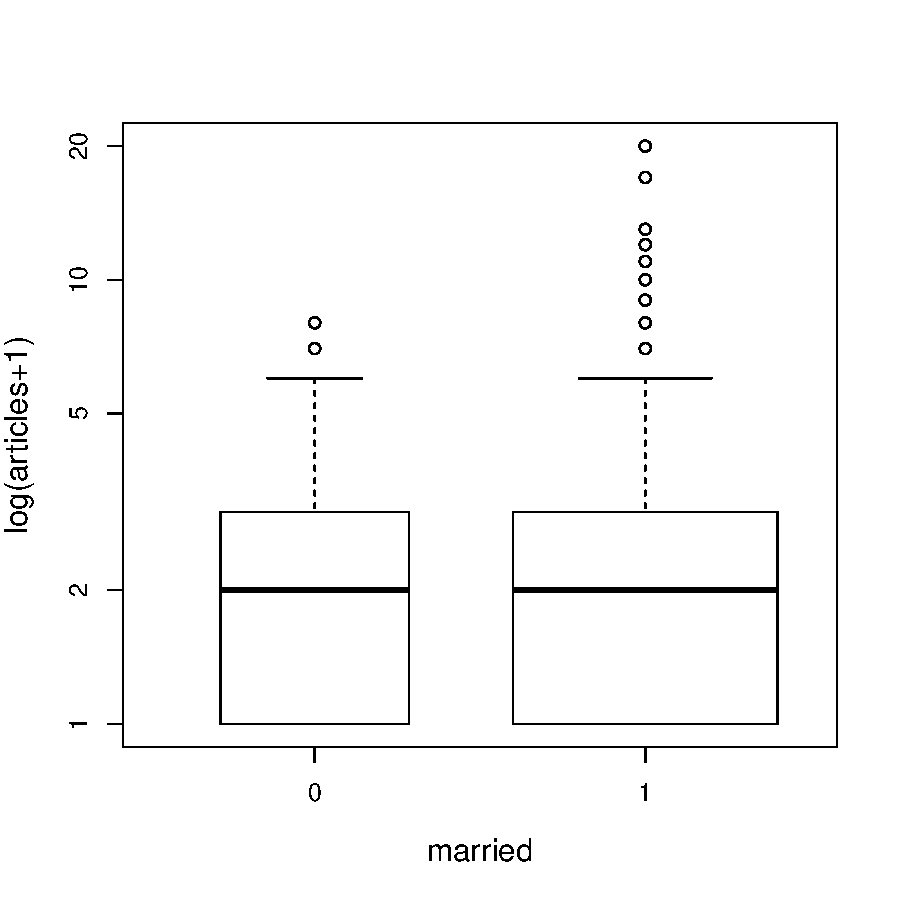
\includegraphics[width=.49\textwidth]{ch09/fig/phdpubs-logplots-1} 
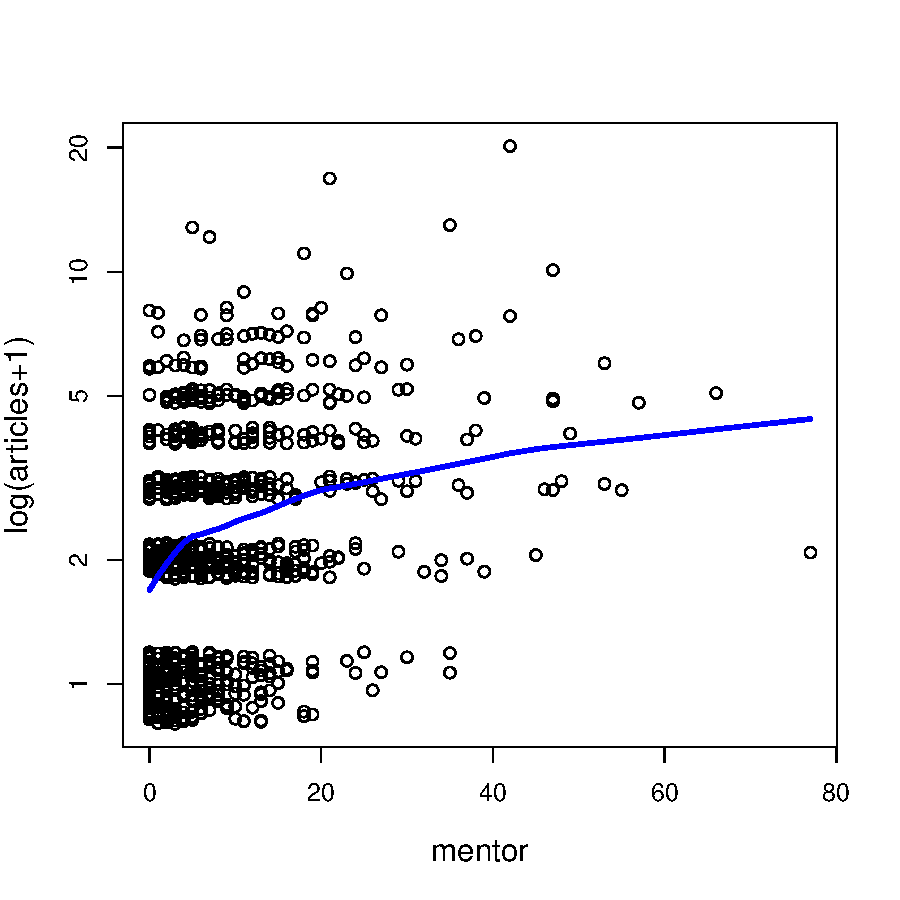
\includegraphics[width=.49\textwidth]{ch09/fig/phdpubs-logplots-2} }

\caption[Exploratory plots for the number of articles in the PhdPubs data]{Exploratory plots for the number of articles in the PhdPubs data. Left: boxplots for married (1) vs. non-married (0); right: jittered scatterplot vs. mentor publications with a lowess smoothed curve.\label{fig:phdpubs-logplots}}
\end{figure}


\end{knitrout}
It can be seen that the distribution of articles for married and non-married are quite similar,
except that for the married students there are quite a few observations with a large number
of publications.  The relationship between log(articles) and mentor publications seems largely
linear except possibly at the very low end.  The large number of zero counts at the lower left
corner stands out; this would not be seen without jittering.

Plots similar to those in \figref{fig:phdpubs-logplots} can also be produced using \pkg{ggplot2}
with greater flexibility, but perhaps greater effort to get the details right.
One key feature is the use of \func{scale\_y\_log10} to plot the response, and all other
features on a log scale.
The following code gives a plot similar to the right panel of
\figref{fig:phdpubs-logplots}, but also plots a confidence band around the smoothed curve,
and adds a linear regression line of log(articles) on mentor publications.  This plot
is not shown here, but it is a good exercise to reproduce it for yourself.

\begin{knitrout}
\definecolor{shadecolor}{rgb}{1, 0.961, 0.933}\color{fgcolor}\begin{kframe}
\begin{alltt}
\hlkwd{ggplot}\hlstd{(PhdPubs,} \hlkwd{aes}\hlstd{(mentor, articles}\hlopt{+}\hlnum{1}\hlstd{))} \hlopt{+}
  \hlkwd{geom_jitter}\hlstd{(}\hlkwc{position}\hlstd{=}\hlkwd{position_jitter}\hlstd{(}\hlkwc{h}\hlstd{=}\hlnum{0.05}\hlstd{))} \hlopt{+}
  \hlkwd{stat_smooth}\hlstd{(}\hlkwc{method}\hlstd{=}\hlstr{"loess"}\hlstd{,} \hlkwc{size}\hlstd{=}\hlnum{2}\hlstd{,} \hlkwc{fill}\hlstd{=}\hlstr{"blue"}\hlstd{,} \hlkwc{alpha}\hlstd{=}\hlnum{0.25}\hlstd{)} \hlopt{+}
        \hlkwd{stat_smooth}\hlstd{(}\hlkwc{method}\hlstd{=}\hlstr{"lm"}\hlstd{,} \hlkwc{color}\hlstd{=}\hlstr{"red"}\hlstd{,} \hlkwc{size}\hlstd{=}\hlnum{1.25}\hlstd{,} \hlkwc{se}\hlstd{=}\hlnum{FALSE}\hlstd{)} \hlopt{+}
        \hlkwd{scale_y_log10}\hlstd{(}\hlkwc{breaks}\hlstd{=}\hlkwd{c}\hlstd{(}\hlnum{1}\hlstd{,}\hlnum{2}\hlstd{,}\hlnum{5}\hlstd{,}\hlnum{10}\hlstd{,}\hlnum{20}\hlstd{))} \hlopt{+}
        \hlkwd{labs}\hlstd{(}\hlkwc{y} \hlstd{=} \hlstr{"log (articles+1)"}\hlstd{,} \hlkwc{x}\hlstd{=}\hlstr{"Mentor publications"}\hlstd{)}
\end{alltt}
\end{kframe}
\end{knitrout}


To start analysis, we fit the Poisson model using all predictors---
\code{female}, \code{married}, \code{kid5}, \code{phdprestige}, and
\code{mentor}. As recorded in \data{PhdPubs}, \code{female} and
\code{married} are both dummy (0/1) variables, and it slightly
more convenient for plotting purposes to make them factors.

\begin{knitrout}
\definecolor{shadecolor}{rgb}{1, 0.961, 0.933}\color{fgcolor}\begin{kframe}
\begin{alltt}
\hlstd{PhdPubs} \hlkwb{<-} \hlkwd{within}\hlstd{(PhdPubs, \{}
  \hlstd{female} \hlkwb{<-} \hlkwd{factor}\hlstd{(female)}
  \hlstd{married} \hlkwb{<-} \hlkwd{factor}\hlstd{(married)}
\hlstd{\})}
\end{alltt}
\end{kframe}
\end{knitrout}

The model is fit as shown below and summarized using \func{summary}, but with abbreviated output.
\begin{knitrout}
\definecolor{shadecolor}{rgb}{1, 0.961, 0.933}\color{fgcolor}\begin{kframe}
\begin{alltt}
\hlstd{phd.pois} \hlkwb{<-} \hlkwd{glm}\hlstd{(articles} \hlopt{~} \hlstd{.,} \hlkwc{data}\hlstd{=PhdPubs,} \hlkwc{family}\hlstd{=poisson)}
\hlkwd{summary}\hlstd{(phd.pois)}
\end{alltt}
\begin{verbatim}
...
## Coefficients:
##             Estimate Std. Error z value Pr(>|z|)    
## (Intercept)  0.26562    0.09962    2.67   0.0077 ** 
## female1     -0.22442    0.05458   -4.11  3.9e-05 ***
## married1     0.15732    0.06125    2.57   0.0102 *  
## kid5        -0.18491    0.04012   -4.61  4.0e-06 ***
## phdprestige  0.02538    0.02527    1.00   0.3153    
## mentor       0.02523    0.00203   12.43  < 2e-16 ***
## ---
## Signif. codes:  0 '***' 0.001 '**' 0.01 '*' 0.05 '.' 0.1 ' ' 1
## 
## (Dispersion parameter for poisson family taken to be 1)
## 
##     Null deviance: 1817.4  on 914  degrees of freedom
## Residual deviance: 1633.6  on 909  degrees of freedom
## AIC: 3313
...
\end{verbatim}
\end{kframe}
\end{knitrout}
Significance tests for the individual coefficients show that all are significant,
except for \code{phdprestige}.  We ignore this here, and continue to interpret and
extend the full main effects model.%
\footnote{
It is usually less harmful to include a non-significant predictor,
(which in any case may be a variable useful to control, as \code{phdprestige} here), than to omit a
potentially important predictor, or worse--- to fail to account for an important interaction.
}

The estimated coefficients $\vec{\beta}$ for the predictors are shown below.
Recall that using the log link means, for example, that being married increases
the log of the expected number of
articles published by 0.157, holding all other predictors constant.
Each additional child of age 5 or less decreases this by 0.185.
\begin{knitrout}
\definecolor{shadecolor}{rgb}{1, 0.961, 0.933}\color{fgcolor}\begin{kframe}
\begin{alltt}
\hlkwd{round}\hlstd{(}\hlkwd{cbind}\hlstd{(}\hlkwc{beta}\hlstd{=}\hlkwd{coef}\hlstd{(phd.pois),}
            \hlkwc{expbeta}\hlstd{=}\hlkwd{exp}\hlstd{(}\hlkwd{coef}\hlstd{(phd.pois)),}
            \hlkwc{pct}\hlstd{=}\hlnum{100}\hlopt{*}\hlstd{(}\hlkwd{exp}\hlstd{(}\hlkwd{coef}\hlstd{(phd.pois))}\hlopt{-}\hlnum{1}\hlstd{)),}\hlnum{3}\hlstd{)}
\end{alltt}
\begin{verbatim}
##               beta expbeta     pct
## (Intercept)  0.266   1.304  30.425
## female1     -0.224   0.799 -20.102
## married1     0.157   1.170  17.037
## kid5        -0.185   0.831 -16.882
## phdprestige  0.025   1.026   2.570
## mentor       0.025   1.026   2.555
\end{verbatim}
\end{kframe}
\end{knitrout}
\noindent It is somewhat easier to interpret the exponentiated coefficients, $\exp(\vec{\beta})$
as multiplicative effects on the expected number of articles and convert these to percentage
change, again holding other predictors constant.
For example, expected publications by married candidates are 1.17 times that of non-married,
a 17\% increase, while each additional child multiplies articles by 0.831, a 16.88\% decrease.

Alternatively, we recommend visual displays for model interpretation, and effect plots do well
in most cases, as shown in  \figref{fig:phdpubs1-effpois}.
For a Poisson GLM, an important feature is that the response is plotted on
the log scale, so that effects in the model appear as linear functions, while the
values of the response (number of articles) are labeled on their original scale, facilitating
interpretation. The confidence bands and error bars give 95\% confidence intervals
around the fitted effects.

\begin{knitrout}
\definecolor{shadecolor}{rgb}{1, 0.961, 0.933}\color{fgcolor}\begin{kframe}
\begin{alltt}
\hlkwd{library}\hlstd{(effects)}
\hlkwd{plot}\hlstd{(}\hlkwd{allEffects}\hlstd{(phd.pois),} \hlkwc{band.colors}\hlstd{=}\hlstr{"blue"}\hlstd{,} \hlkwc{lwd}\hlstd{=}\hlnum{3}\hlstd{,}
     \hlkwc{ylab}\hlstd{=}\hlstr{"Number of articles"}\hlstd{,} \hlkwc{main}\hlstd{=}\hlstr{""}\hlstd{)}
\end{alltt}
\end{kframe}\begin{figure}[!htbp]


\centerline{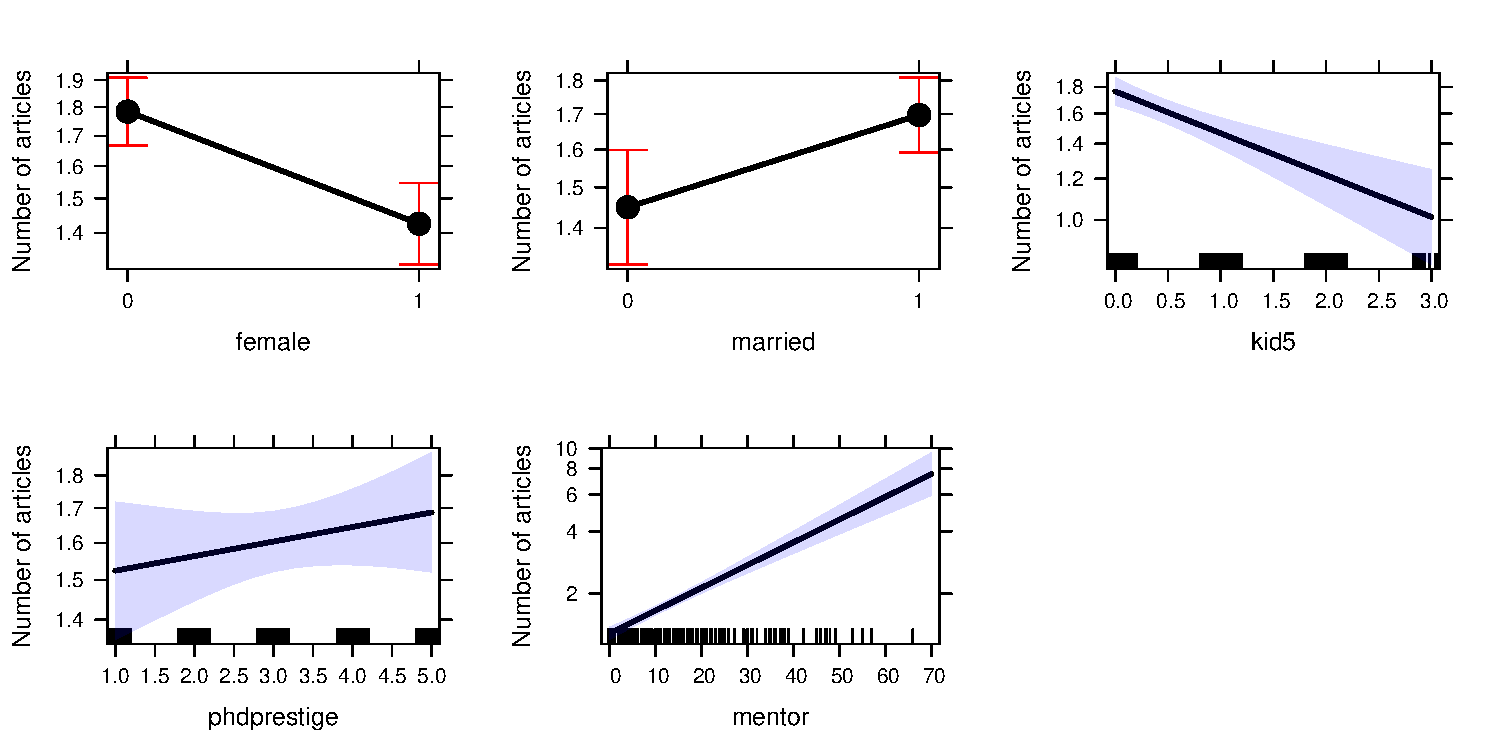
\includegraphics[width=\textwidth]{ch09/fig/phdpubs1-effpois-1} }

\caption[Effect plots for the predictors in the Poisson regression model for the PhdPubs data]{Effect plots for the predictors in the Poisson regression model for the PhdPubs data. Jittered values of the continuous predictors are shown at the bottom as rug-plots.\label{fig:phdpubs1-effpois}}
\end{figure}


\end{knitrout}

In \figref{fig:phdpubs1-effpois} we can see the decrease in published articles with
number of young children, but also that the confidence band gets wider with increasing
children.  The predicted effect here of number of publications by the student's mentor is more
dramatic, particularly for those whose mentor were truly prolific.

You should note that the panels for the predictors in \figref{fig:phdpubs1-effpois} are scaled
individually for the range of the fitted main effects.  This is often a sensible default
and all predictors except \code{mentor} give a similar range here.  To make all of these
plots strictly comparable, provide a \code{ylim} argument, giving the range of the
response on the log scale, as below (but not shown here).
\begin{knitrout}
\definecolor{shadecolor}{rgb}{1, 0.961, 0.933}\color{fgcolor}\begin{kframe}
\begin{alltt}
\hlkwd{plot}\hlstd{(}\hlkwd{allEffects}\hlstd{(phd.pois),} \hlkwc{band.colors}\hlstd{=}\hlstr{"blue"}\hlstd{,} \hlkwc{ylim}\hlstd{=}\hlkwd{c}\hlstd{(}\hlnum{0}\hlstd{,}\hlkwd{log}\hlstd{(}\hlnum{10}\hlstd{)))}
\end{alltt}
\end{kframe}
\end{knitrout}

All of the above is useful, but still leaves aside the question of how well the Poisson model fits
the data. The output from \code{summary(phd.pois)} above showed that the Poisson model fits quite badly.
The residual deviance of 1633.6 with 909 degrees
of freedom is highly significant.

\end{Example}



\begin{Example}[crabs1]{Mating of horseshoe crabs}
\citet{Brockmann:1996} studied the mating behavior of female horseshoe crabs in the Gulf of Mexico.
In the mating season, crabs arrive on the beach in female/male pairs to lay and fertilize eggs.
However, unattached males, called ``satellites,''
also come to the beach, crowd around the nesting couples and compete with attached males for fertilizations,
contributing to reproductive success.
Some females are ignored by satellite males, and some attract
more satellites than others, and the question is: what factors contribute to
to the number of satellites for each female? Or, perhaps better, how do unattached males choose among
available females?
This is another example in which zero counts
may require special treatment.

The data, given in \data{CrabSatellites} in the \Rpackage{countreg}, give the
response variable, \code{satellites} for 173 females.  Possible predictors
are the female's \code{color} and \code{spine} condition, given as ordered factors,
as well as her \code{weight} and carapace (shell) \code{width}.

\begin{knitrout}\footnotesize
\definecolor{shadecolor}{rgb}{1, 0.961, 0.933}\color{fgcolor}\begin{kframe}
\begin{alltt}
\hlkwd{data}\hlstd{(}\hlstr{"CrabSatellites"}\hlstd{,} \hlkwc{package} \hlstd{=} \hlstr{"countreg"}\hlstd{)}
\hlkwd{str}\hlstd{(CrabSatellites)}
\end{alltt}
\begin{verbatim}
## 'data.frame':	173 obs. of  5 variables:
##  $ color     : Ord.factor w/ 4 levels "lightmedium"<..: 2 3 3 4 2 1 4 2 2 2 ...
##  $ spine     : Ord.factor w/ 3 levels "bothgood"<"onebroken"<..: 3 3 3 2 3 2 3 3 1 3 ...
##  $ width     : num  28.3 26 25.6 21 29 25 26.2 24.9 25.7 27.5 ...
##  $ weight    : num  3.05 2.6 2.15 1.85 3 2.3 1.3 2.1 2 3.15 ...
##  $ satellites: int  8 4 0 0 1 3 0 0 8 6 ...
\end{verbatim}
\end{kframe}
\end{knitrout}

\citet[\S 4.3]{Agresti:2013} analyses the number of satellites using count data
GLMs, and in his \C 5, describes separate logistic regression models for the binary
outcome of one or more satellites vs.\ none.  Later in this chapter (\secref{sec:glm-zeros})
we consider
hurdle and zero-inflated models for count data.  These have the advantage of
modeling the zero counts together with a model for the positive counts.

A useful overview plot of the data is shown using \func{gpairs} in \figref{fig:crabs1-gpairs}.
You can see that the distribution of \var{satellites} is quite positively skewed,
with many zero counts.  \var{width} and \var{weight} are highly correlated (0.89),
and both relate to the size of the female.
Their scatterplots in the first row show that larger females attract more satellites.
The categorical ordered factors \var{spine} condition and \var{color} are strongly
associated, with the lightest colored crabs having the best conditions.
\begin{knitrout}
\definecolor{shadecolor}{rgb}{1, 0.961, 0.933}\color{fgcolor}\begin{kframe}
\begin{alltt}
\hlkwd{library}\hlstd{(vcd)}
\hlkwd{library}\hlstd{(gpairs)}
\hlkwd{gpairs}\hlstd{(CrabSatellites[,}\hlnum{5}\hlopt{:}\hlnum{1}\hlstd{],}
       \hlkwc{diag.pars} \hlstd{=} \hlkwd{list}\hlstd{(}\hlkwc{fontsize}\hlstd{=}\hlnum{16}\hlstd{),}
       \hlkwc{mosaic.pars} \hlstd{=} \hlkwd{list}\hlstd{(}\hlkwc{gp}\hlstd{=shading_Friendly,} \hlkwc{gp_args}\hlstd{=}\hlkwd{list}\hlstd{(}\hlkwc{interpolate}\hlstd{=}\hlnum{1}\hlopt{:}\hlnum{4}\hlstd{)))}
\end{alltt}
\end{kframe}\begin{figure}[!htbp]


\centerline{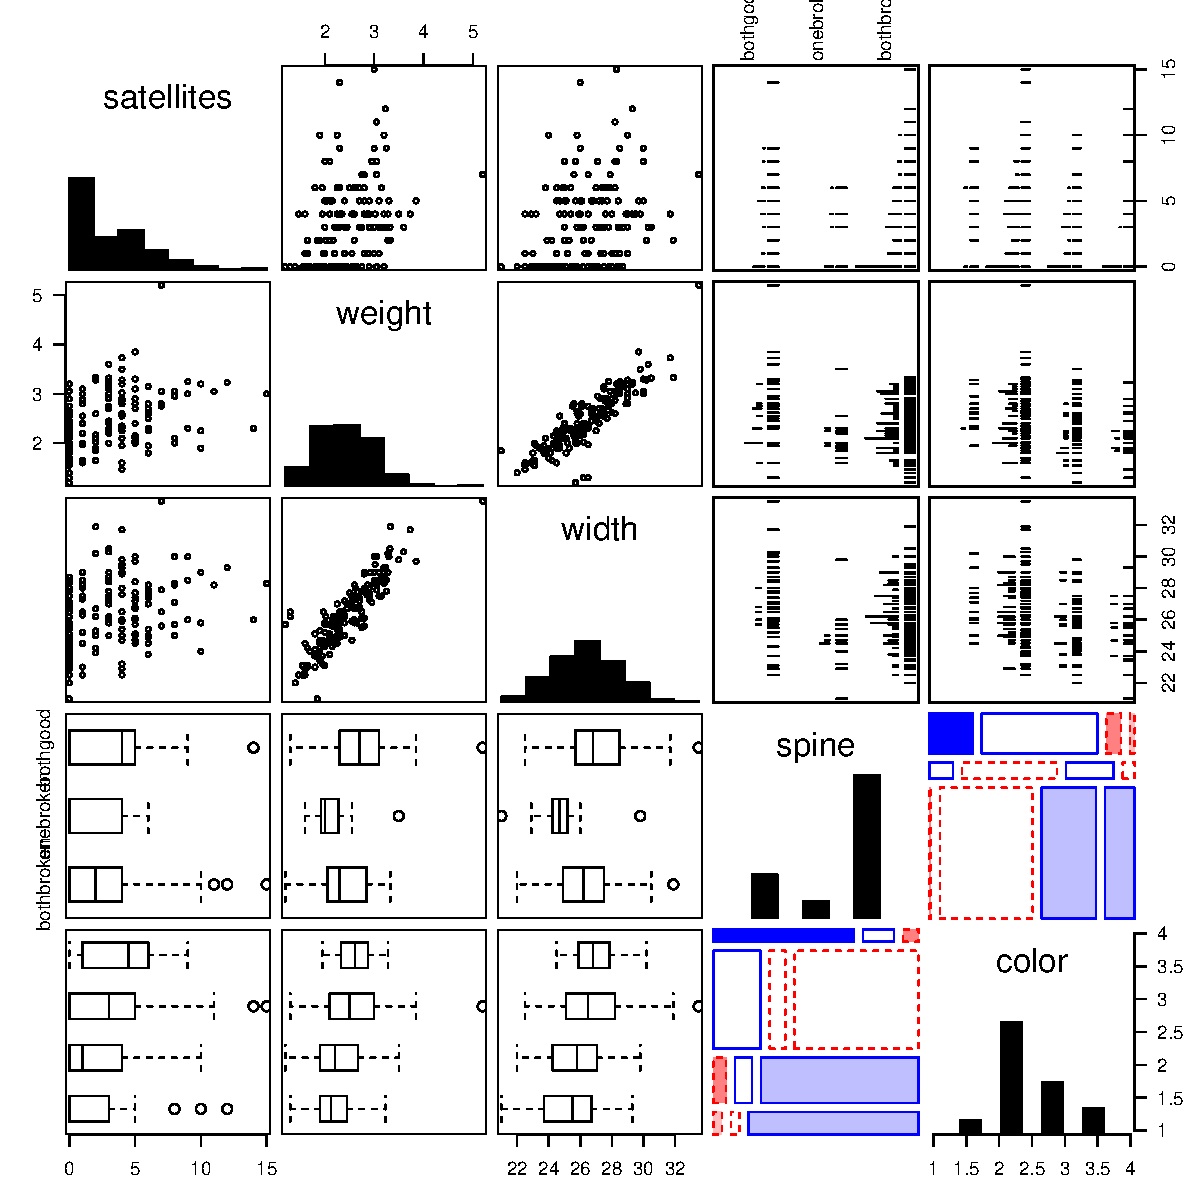
\includegraphics[width=.8\textwidth]{ch09/fig/crabs1-gpairs-1} }

\caption[Generalized pairs plot for the CrabSatellites data]{Generalized pairs plot for the CrabSatellites data.\label{fig:crabs1-gpairs}}
\end{figure}


\end{knitrout}

\figref{fig:crabs1-scats} shows the scatterplots of \var{satellites} against \var{width} and \var{weight}
together with smoothed lowess curves.
\begin{knitrout}
\definecolor{shadecolor}{rgb}{1, 0.961, 0.933}\color{fgcolor}\begin{kframe}
\begin{alltt}
\hlkwd{plot}\hlstd{(}\hlkwd{jitter}\hlstd{(satellites)} \hlopt{~} \hlstd{width,} \hlkwc{data}\hlstd{=CrabSatellites,}
  \hlkwc{ylab}\hlstd{=}\hlstr{"Number of satellites (jittered)"}\hlstd{,} \hlkwc{xlab}\hlstd{=}\hlstr{"Carapace width"}\hlstd{,}
  \hlkwc{cex.lab}\hlstd{=}\hlnum{1.25}\hlstd{)}
\hlkwd{with}\hlstd{(CrabSatellites,} \hlkwd{lines}\hlstd{(}\hlkwd{lowess}\hlstd{(width, satellites),} \hlkwc{col}\hlstd{=}\hlstr{"red"}\hlstd{,} \hlkwc{lwd}\hlstd{=}\hlnum{2}\hlstd{))}
\hlkwd{plot}\hlstd{(}\hlkwd{jitter}\hlstd{(satellites)} \hlopt{~} \hlstd{weight,} \hlkwc{data}\hlstd{=CrabSatellites,}
  \hlkwc{ylab}\hlstd{=}\hlstr{"Number of satellites (jittered)"}\hlstd{,} \hlkwc{xlab}\hlstd{=}\hlstr{"Weight"}\hlstd{,}
  \hlkwc{cex.lab}\hlstd{=}\hlnum{1.25}\hlstd{)}
\hlkwd{with}\hlstd{(CrabSatellites,} \hlkwd{lines}\hlstd{(}\hlkwd{lowess}\hlstd{(weight, satellites),} \hlkwc{col}\hlstd{=}\hlstr{"red"}\hlstd{,} \hlkwc{lwd}\hlstd{=}\hlnum{2}\hlstd{))}
\end{alltt}
\end{kframe}\begin{figure}[!htbp]


\centerline{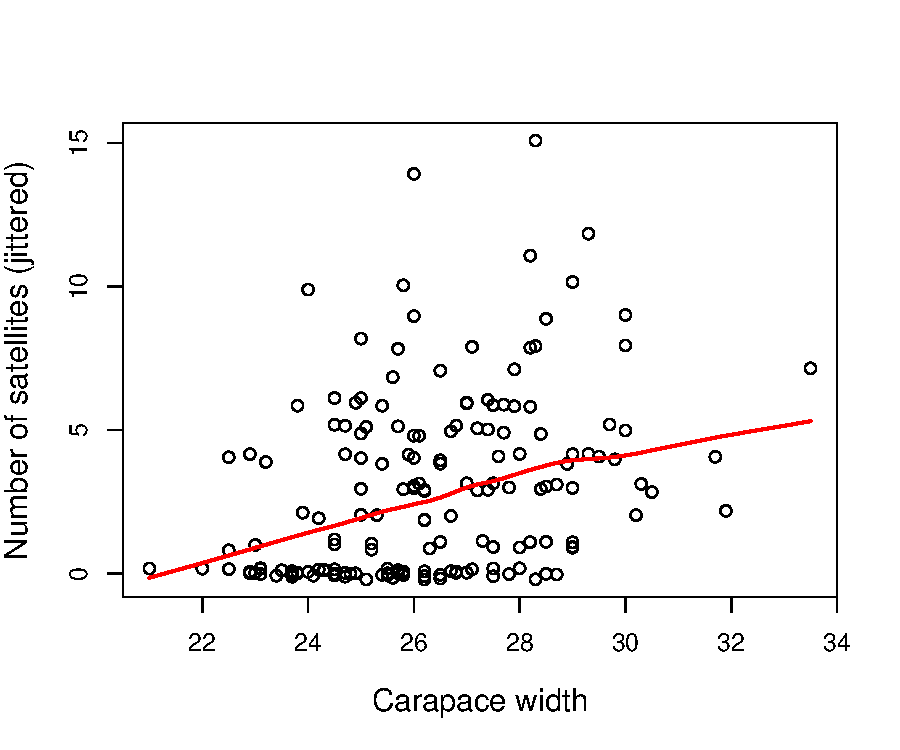
\includegraphics[width=.49\textwidth]{ch09/fig/crabs1-scats-1} 
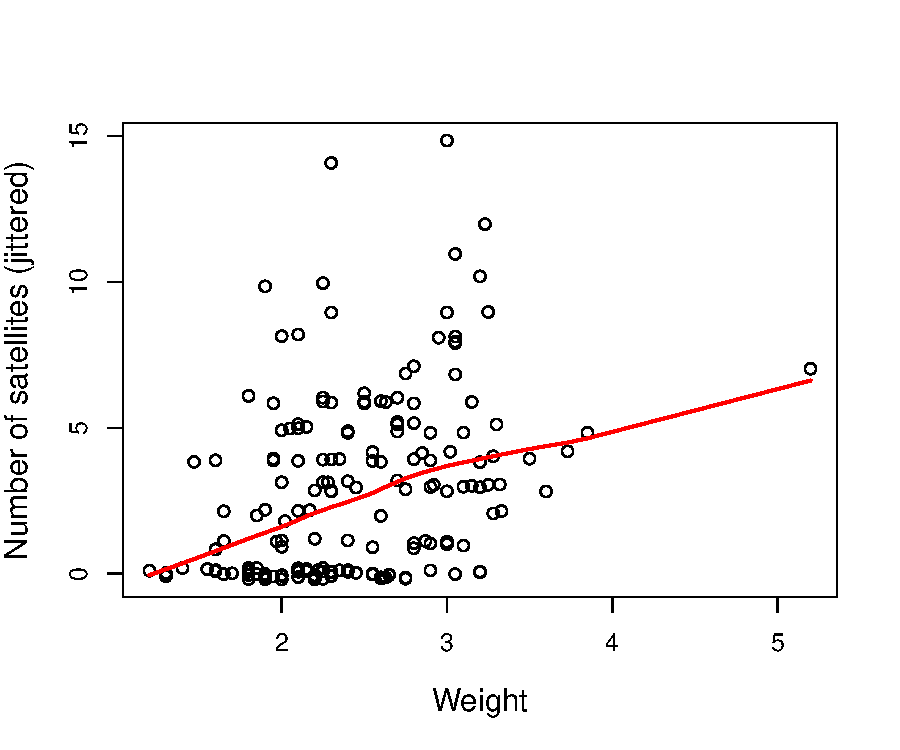
\includegraphics[width=.49\textwidth]{ch09/fig/crabs1-scats-2} }

\caption[Scatterplots of number of satellites vs]{Scatterplots of number of satellites vs. width and weight, with lowess smooths.\label{fig:crabs1-scats}}
\end{figure}


\end{knitrout}
Both variables show approximately linear relations to the mean number of satellites, so it
would not be unreasonable to fit models using the identity link ($\mu \sim x$) rather than the log link
($\mu \sim \log(x)$) with the Poisson family GLM.

In these plots, we reduce the problem of overplotting of the discrete response by jittering, but
an alternative technique is to transform a numeric count or continuous predictor to
a factor (for visualization purposes only), thereby giving boxplots.  A convenience function for
this purpose, \func{cutfac} is defined in \pkg{vcdExtra}.  
It acts like \func{cut}, but gives nicer labels
for the factor levels and by default chooses convenient breaks among the values based on deciles.
% 
% <<cutfac, size='footnotesize'>>=
% cutfac <- function(x, breaks = NULL, q=10) {
%   if(is.null(breaks)) breaks <- unique(quantile(x, 0:q/q))
%   x <- cut(x, breaks, include.lowest = TRUE, right = FALSE)
%   levels(x) <- paste(breaks[-length(breaks)], ifelse(diff(breaks) > 1,
%     c(paste("-", breaks[-c(1, length(breaks))] - 1, sep = ""), "+"), ""), sep = "")
%   return(x)
% }
% @
% 
Using this, the plots in \figref{fig:crabs1-scats} can be re-drawn as boxplots, giving \figref{fig:crabs1-boxplots}.

\begin{knitrout}
\definecolor{shadecolor}{rgb}{1, 0.961, 0.933}\color{fgcolor}\begin{kframe}
\begin{alltt}
\hlkwd{plot}\hlstd{(satellites} \hlopt{~} \hlkwd{cutfac}\hlstd{(width),} \hlkwc{data}\hlstd{=CrabSatellites,}
     \hlkwc{ylab}\hlstd{=}\hlstr{"Number of satellites"}\hlstd{,} \hlkwc{xlab}\hlstd{=}\hlstr{"Carapace width (deciles)"}\hlstd{)}
\hlkwd{plot}\hlstd{(satellites} \hlopt{~} \hlkwd{cutfac}\hlstd{(weight),} \hlkwc{data}\hlstd{=CrabSatellites,}
     \hlkwc{ylab}\hlstd{=}\hlstr{"Number of satellites"}\hlstd{,} \hlkwc{xlab}\hlstd{=}\hlstr{"Weight (deciles)"}\hlstd{)}
\end{alltt}
\end{kframe}\begin{figure}[!htbp]


\centerline{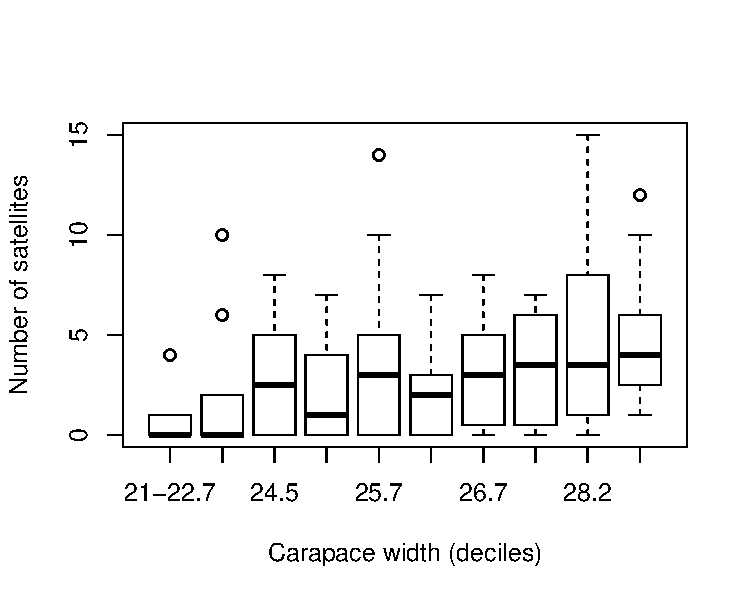
\includegraphics[width=.49\textwidth]{ch09/fig/crabs1-boxplots-1} 
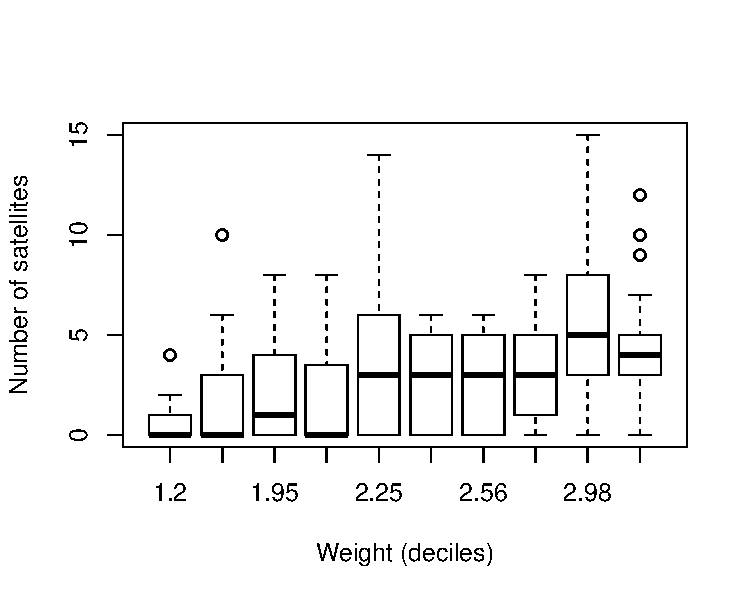
\includegraphics[width=.49\textwidth]{ch09/fig/crabs1-boxplots-2} }

\caption[Boxplots of number of satellites vs]{Boxplots of number of satellites vs. width and weight.\label{fig:crabs1-boxplots}}
\end{figure}


\end{knitrout}

With this visual overview, we proceed to an initial Poisson GLM model, using all predictors.
Note that \var{color} and \var{spine} are ordered factors, so \func{glm} represents them
as polynomial contrasts, as if they were coded numerically.

\begin{knitrout}
\definecolor{shadecolor}{rgb}{1, 0.961, 0.933}\color{fgcolor}\begin{kframe}
\begin{alltt}
\hlstd{crabs.pois} \hlkwb{<-} \hlkwd{glm}\hlstd{(satellites} \hlopt{~} \hlstd{.,} \hlkwc{data}\hlstd{=CrabSatellites,} \hlkwc{family}\hlstd{=poisson)}
\hlkwd{summary}\hlstd{(crabs.pois)}
\end{alltt}
\begin{verbatim}
...
## Coefficients:
##             Estimate Std. Error z value Pr(>|z|)   
## (Intercept)  -0.7057     0.9344   -0.76   0.4501   
## color.L      -0.4120     0.1567   -2.63   0.0085 **
## color.Q       0.1237     0.1231    1.00   0.3150   
## color.C       0.0481     0.0914    0.53   0.5983   
## spine.L       0.0618     0.0848    0.73   0.4660   
## spine.Q       0.1585     0.1609    0.99   0.3244   
## width         0.0165     0.0489    0.34   0.7358   
## weight        0.4971     0.1663    2.99   0.0028 **
## ---
## Signif. codes:  0 '***' 0.001 '**' 0.01 '*' 0.05 '.' 0.1 ' ' 1
## 
## (Dispersion parameter for poisson family taken to be 1)
## 
##     Null deviance: 632.79  on 172  degrees of freedom
## Residual deviance: 549.56  on 165  degrees of freedom
## AIC: 920.9
...
\end{verbatim}
\end{kframe}
\end{knitrout}
The Wald tests for the coefficients show that only the linear effect of color and the effect
of width are significant.
Effect plots, in \figref{fig:crabs1-eff1}, show the nature of these
effects--- lighter colored females attract more satellites, as do wider and heavier females.

\begin{knitrout}
\definecolor{shadecolor}{rgb}{1, 0.961, 0.933}\color{fgcolor}\begin{kframe}
\begin{alltt}
\hlkwd{plot}\hlstd{(}\hlkwd{allEffects}\hlstd{(crabs.pois),} \hlkwc{main}\hlstd{=}\hlstr{""}\hlstd{)}
\end{alltt}
\end{kframe}\begin{figure}[!htbp]


\centerline{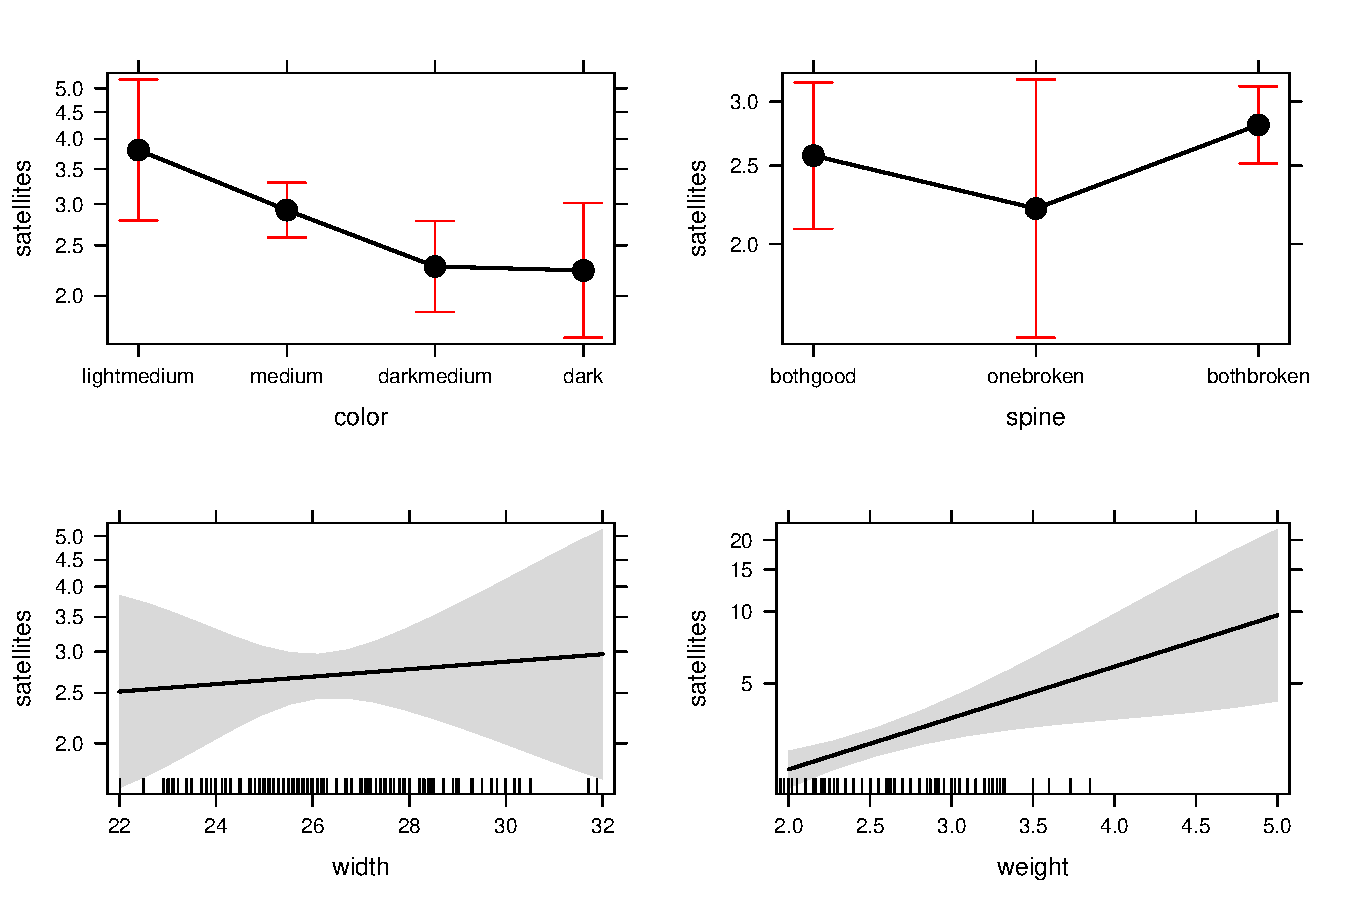
\includegraphics[width=\textwidth]{ch09/fig/crabs1-eff1-1} }

\caption[Effect plots for the predictors in the Poisson regression model for the CrabSatellites data]{Effect plots for the predictors in the Poisson regression model for the CrabSatellites data.\label{fig:crabs1-eff1}}
\end{figure}


\end{knitrout}

A simpler model can be constructed using \var{color} as a numeric variable, and either width or
weight to represent female size. We choose weight here.%
\footnote{
\citet[\S 4.3]{Agresti:2013} and others who have analyzed this example uses carapace width
as the main quantitative predictor, possibly because width might be more biologically salient
to the single males than weight.  This is a case where two
highly correlated predictors are each strongly related to the outcome,
yet partial tests (controlling for all others) may prefer one over the other.
}

\begin{knitrout}
\definecolor{shadecolor}{rgb}{1, 0.961, 0.933}\color{fgcolor}\begin{kframe}
\begin{alltt}
\hlstd{CrabSatellites1} \hlkwb{<-} \hlkwd{transform}\hlstd{(CrabSatellites,}
  \hlkwc{color} \hlstd{=} \hlkwd{as.numeric}\hlstd{(color))}

\hlstd{crabs.pois1} \hlkwb{<-} \hlkwd{glm}\hlstd{(satellites} \hlopt{~} \hlstd{weight} \hlopt{+} \hlstd{color,} \hlkwc{data}\hlstd{=CrabSatellites1,}
                   \hlkwc{family}\hlstd{=poisson)}
\hlkwd{summary}\hlstd{(crabs.pois1)}
\end{alltt}
\begin{verbatim}
...
## 
## Coefficients:
##             Estimate Std. Error z value Pr(>|z|)    
## (Intercept)   0.0888     0.2544    0.35    0.727    
## weight        0.5458     0.0675    8.09    6e-16 ***
## color        -0.1728     0.0615   -2.81    0.005 ** 
## ---
## Signif. codes:  0 '***' 0.001 '**' 0.01 '*' 0.05 '.' 0.1 ' ' 1
## 
## (Dispersion parameter for poisson family taken to be 1)
## 
##     Null deviance: 632.79  on 172  degrees of freedom
## Residual deviance: 552.77  on 170  degrees of freedom
## AIC: 914.1
...
\end{verbatim}
\end{kframe}
\end{knitrout}

From the statistical and graphical analysis so far, the answer to the question posed
in this example is clear:  unattached male horseshoe crabs prefer light-colored
big, fat mamas!

Yet, neither of these models fit well, as can be seen from their residual deviances
and \LR tests.
\begin{knitrout}
\definecolor{shadecolor}{rgb}{1, 0.961, 0.933}\color{fgcolor}\begin{kframe}
\begin{alltt}
\hlstd{vcdExtra::}\hlkwd{Summarise}\hlstd{(crabs.pois, crabs.pois1)}
\end{alltt}
\begin{verbatim}
## Likelihood summary table:
##             AIC BIC LR Chisq  Df Pr(>Chisq)    
## crabs.pois  921 946      550 165     <2e-16 ***
## crabs.pois1 914 924      553 170     <2e-16 ***
## ---
## Signif. codes:  0 '***' 0.001 '**' 0.01 '*' 0.05 '.' 0.1 ' ' 1
\end{verbatim}
\end{kframe}
\end{knitrout}
Perhaps there is something else to be learned here.

\end{Example} 

\section{Models for overdispersed count data}\label{sec:glm-overdisp}

In practice, the Poisson model is often very useful for describing the
relationship between the mean $\mu_i$ and the linear predictors,
but typically underestimates the variance in the data.
The consequence is that the Poisson standard errors are too small,
rendering the Wald tests of coefficients, $z_j = \widehat{\beta}_j / \mathrm{se} (\widehat{\beta}_j) $
(and other hypothesis test statistics)
too large, and thus overly liberal.

In applications of the GLM, overdispersion is usually assessed by the \LR
test of the deviance (or the Pearson statistic) given in \secref{sec:glm-goodfit},
but there is a subtle problem here. Lack of fit in a GLM for count data can result
either from a mis-specified model for the systematic component
(omitted or unmeasured predictors, non-linear relations, etc.)
or from failure of the Poisson mean = variance assumption.
Thus, use of these methods requires some high degree of confidence that the
systematic part of the model has been correctly specified, so that any
lack of fit can be attributed to overdispersion.

One way of dealing with this is to base inference on
so-called \emph{sandwich} covariance estimators that are robust against
some types of model mis-specification.  In \R, this is provided by the
\func{sandwich} function in the \Rpackage{sandwich}, and can be used
with \code{coeftest(model, vcov=sandwich)} to give overdispersion-corrected
hypothesis tests.
Alternatively, the Poisson model variance assumption can be relaxed
in the quasi-Poisson model and the negative-binomial model as
discussed below.


\subsection{The quasi-Poisson model}\label{sec:glm-quasi}

One obvious solution to the problem of overdispersion for count data is the relaxed assumption
that the conditional variance is merely \emph{proportional} to the mean,
\begin{equation*}
\V (y_i | \eta_i) = \phi \mu_i
\end{equation*}
Overdispersion is the common case of $\phi > 1$, implying that the conditional variance
increases faster than the mean, but the opposite case of underdispersion, $\phi < 1$
is also possible, though relatively rare in practice.
This strategy entails estimating the dispersion parameter $\phi$ from the data,
and gives the \term{quasi-Poisson model} for count data.

One possible estimate is the residual deviance divided by degrees of freedom.
However, it is more common to use the Pearson statistics, that gives
a method-of-moments estimate with improved statistical properties.
\begin{equation*}
\widehat{\phi} =
\frac{X^2_P}{n-p} =
\sum_{i=1}^n \frac{(y_i - \widehat{\mu}_i)^2}{\widehat{\mu}_i} \left/ (n-p) \right.
\end{equation*}

It turns out that this model gives the same coefficient estimates as the standard
Poisson GLM, but inference is adjusted for over/under dispersion.
In particular, following \eqref{eq:varbeta}
the standard errors of the model coefficients are multiplied by
$\widehat{\phi}^{1/2}$ and so are inflated when overdispersion is present.
In \R, the quasi-Poisson model with this estimated dispersion parameter is
fitted with the \func{glm} function, by setting \code{family=quasipoisson}.

\begin{Example}[phdpubs2]{Publications of PhD candidates}

For the \data{PhdPubs} data, the deviance and Pearson estimates of dispersion $\phi$
can be calculated using the results of the Poisson model saved in the
\code{phd.pois} object.  The Pearson estimate, 1.83, indicates that
standard errors of coefficients in this model should be multiplied by
$\sqrt{1.83} = 1.35$, a 35\% increase, to correct for overdispersion.

\begin{knitrout}
\definecolor{shadecolor}{rgb}{1, 0.961, 0.933}\color{fgcolor}\begin{kframe}
\begin{alltt}
\hlkwd{with}\hlstd{(phd.pois, deviance}\hlopt{/}\hlstd{df.residual)}
\end{alltt}
\begin{verbatim}
## [1] 1.7971
\end{verbatim}
\begin{alltt}
\hlkwd{sum}\hlstd{(}\hlkwd{residuals}\hlstd{(phd.pois,} \hlkwc{type} \hlstd{=} \hlstr{"pearson"}\hlstd{)}\hlopt{^}\hlnum{2}\hlstd{)}\hlopt{/}\hlstd{phd.pois}\hlopt{$}\hlstd{df.residual}
\end{alltt}
\begin{verbatim}
## [1] 1.8304
\end{verbatim}
\end{kframe}
\end{knitrout}
The quasi-Poisson model is then fitted using \func{glm} as:
\begin{knitrout}
\definecolor{shadecolor}{rgb}{1, 0.961, 0.933}\color{fgcolor}\begin{kframe}
\begin{alltt}
\hlstd{phd.qpois} \hlkwb{<-} \hlkwd{glm}\hlstd{(articles} \hlopt{~} \hlstd{.,} \hlkwc{data}\hlstd{=PhdPubs,} \hlkwc{family}\hlstd{=quasipoisson)}
\end{alltt}
\end{kframe}
\end{knitrout}
For use in other computation, the  dispersion parameter estimate $\widehat{\phi}$ can be obtained as the
\code{dispersion} value of the \func{summary} method for a quasi-Poisson model.
\begin{knitrout}
\definecolor{shadecolor}{rgb}{1, 0.961, 0.933}\color{fgcolor}\begin{kframe}
\begin{alltt}
\hlstd{(phi} \hlkwb{<-} \hlkwd{summary}\hlstd{(phd.qpois)}\hlopt{$}\hlstd{dispersion)}
\end{alltt}
\begin{verbatim}
## [1] 1.8304
\end{verbatim}
\end{kframe}
\end{knitrout}
Note that this value can be compared to the variance/mean ratio of 2.91 calculated for the
marginal distribution in \exref{ex:phdpubs1}; there is considerable improvement taking the
predictors into account.

\end{Example}

\subsection{The negative-binomial model}\label{sec:glm-negbin}

The negative-binomial (NB) model for count data was introduced in \secref{sec:negbin}
as a different generalization of the Poisson model that allows for overdispersion.
In the context of the GLM, this can be developed as the extended form where
the distribution of $y_i \given \vec{x}_i$ where the mean $\mu_i$ for fixed
$\vec{x}_i$ can vary across observations $i$ according to a gamma distribution
with mean $\mu_i$ and a constant shape parameter, $\theta$, reflecting the
additional variation due to heterogeneity.

For a fixed value of $\theta$, the negative-binomial is another special case of
the GLM.
The expected value of the response is again
$\E(y_i) = \mu_i$, but the variance function is $\V(y_i) = \mu_i + \mu_i^2 / \theta$,
so the variance of $y$ increases more rapidly than that of the Poisson distribution.
Some authors (e.g., \citet{Agresti:2013,Hilbe:2014}) prefer to parameterize the variance
function in terms of $\alpha = 1/\theta$, giving
\begin{equation*}
\V(y_i) = \mu_i + \mu_i^2 / \theta = \mu_i + \alpha \mu_i^2 \comma
\end{equation*}
so that $\alpha$ is a kind of dispersion parameter.  Note that as $\alpha \rightarrow 0$,
$\V(y_i) \rightarrow \mu_i$ and the negative-binomial converges to the Poisson.

The \Rpackage{MASS} provides the family function \code{negative.binomial(theta)} that
can be used directly with \func{glm} provided that the argument \code{theta} is specified.
One example would be the related geometric distribution (\secref{sec:geometric}),
that is the special case of $\theta=1$. This can be fitted in \R by setting
\code{family=negative.binomial(theta=1)} in the call to \func{glm}.

Most often, $\theta$ is unknown and must be estimated from the data.
In this case, the negative-binomial model is not a special case of the GLM,
but it is possible to obtain maximum likelihood estimates of both
$\vec{\beta}$ and $\theta$, by iteratively estimating $\vec{\beta}$ for fixed $\theta$
and vice-versa. This method is implemented in the \func{glm.nb} in the package \pkg{MASS}.

\begin{Example}[crabs-nbin]{Mating of horseshoe crabs}
For example, for the \data{CrabSatellites} data,
we can fit the general negative-binomial model with
$\theta$ free.
\begin{knitrout}
\definecolor{shadecolor}{rgb}{1, 0.961, 0.933}\color{fgcolor}\begin{kframe}
\begin{alltt}
\hlkwd{library}\hlstd{(MASS)}
\hlstd{crabs.nbin} \hlkwb{<-} \hlkwd{glm.nb}\hlstd{(satellites} \hlopt{~} \hlstd{weight} \hlopt{+} \hlstd{color,} \hlkwc{data}\hlstd{=CrabSatellites1)}
\hlstd{crabs.nbin}\hlopt{$}\hlstd{theta}
\end{alltt}
\begin{verbatim}
## [1] 0.95562
\end{verbatim}
\end{kframe}
\end{knitrout}
The estimated value $\widehat{\theta}$ returned by \func{glm.nb} is not very far from 1.
Hence, we might also consider fixing $\theta=1$, as illustrated below.
\begin{knitrout}
\definecolor{shadecolor}{rgb}{1, 0.961, 0.933}\color{fgcolor}\begin{kframe}
\begin{alltt}
\hlstd{crabs.nbin1} \hlkwb{<-} \hlkwd{glm}\hlstd{(satellites} \hlopt{~} \hlstd{weight} \hlopt{+} \hlstd{color,} \hlkwc{data}\hlstd{=CrabSatellites1,}
                   \hlkwc{family}\hlstd{=}\hlkwd{negative.binomial}\hlstd{(}\hlnum{1}\hlstd{))}
\end{alltt}
\end{kframe}
\end{knitrout}
\end{Example}

% until I finish the negbin section....



\subsection{Visualizing the mean--variance relation}

The quasi-Poisson and negative-binomial models have different variance functions, and one way to
visualize which provides a better fit to the data is to group the data according to the
fitted value of the linear predictor, calculate the mean and variance for each group, and
then plot the variances against the means.
A smoothed curve will then approximate the \emph{empirical} mean--variance relationship.
To this, we can add curves showing the mean--variance function implied by various models.%
\footnote{
This idea and the example that follows was suggested by Germ\'an Rodrigues
in a Stata example given at
\url{http://data.princeton.edu/wws509/stata/overdispersion.html}.
}

\begin{Example}[phdpubs3]{Publications of PhD candidates}
For the \data{PhdPubs} data, the fitted values are obtained with \func{fitted} for the
Poisson and negative binomial models. Either set can be used to categorize the observations
into groups for the purpose of calculating means and variances of the response.


\begin{knitrout}
\definecolor{shadecolor}{rgb}{1, 0.961, 0.933}\color{fgcolor}\begin{kframe}
\begin{alltt}
\hlstd{fit.pois} \hlkwb{<-} \hlkwd{fitted}\hlstd{(phd.pois,} \hlkwc{type}\hlstd{=}\hlstr{"response"}\hlstd{)}
\hlstd{fit.nbin} \hlkwb{<-} \hlkwd{fitted}\hlstd{(phd.nbin,} \hlkwc{type}\hlstd{=}\hlstr{"response"}\hlstd{)}
\end{alltt}
\end{kframe}
\end{knitrout}
Here we use a simpler version of the \func{cutfac} function to group a numeric variable
into quantile-based groups.  \func{cutq} also uses deciles by default, and just uses
simple integer values for the factor labels.
\begin{knitrout}
\definecolor{shadecolor}{rgb}{1, 0.961, 0.933}\color{fgcolor}\begin{kframe}
\begin{alltt}
\hlstd{cutq} \hlkwb{<-} \hlkwa{function}\hlstd{(}\hlkwc{x}\hlstd{,} \hlkwc{q} \hlstd{=} \hlnum{10}\hlstd{) \{}
    \hlstd{quantile} \hlkwb{<-} \hlkwd{cut}\hlstd{(x,} \hlkwc{breaks} \hlstd{=} \hlkwd{quantile}\hlstd{(x,} \hlkwc{probs} \hlstd{=} \hlnum{0}\hlopt{:}\hlstd{q}\hlopt{/}\hlstd{q),}
        \hlkwc{include.lowest} \hlstd{=} \hlnum{TRUE}\hlstd{,} \hlkwc{labels} \hlstd{=} \hlnum{1}\hlopt{:}\hlstd{q)}
    \hlstd{quantile}
\hlstd{\}}
\end{alltt}
\end{kframe}
\end{knitrout}
Using this, we create a variable \code{group} giving 20 quantile groups of the fitted values,
and then use \func{aggregate} to find the mean and variance of the number of articles
in each group.
\begin{knitrout}
\definecolor{shadecolor}{rgb}{1, 0.961, 0.933}\color{fgcolor}\begin{kframe}
\begin{alltt}
\hlstd{group} \hlkwb{<-} \hlkwd{cutq}\hlstd{(fit.nbin,} \hlkwc{q}\hlstd{=}\hlnum{20}\hlstd{)}
\hlstd{qdat} \hlkwb{<-} \hlkwd{aggregate}\hlstd{(PhdPubs}\hlopt{$}\hlstd{articles,}
          \hlkwd{list}\hlstd{(group),}
          \hlkwc{FUN} \hlstd{=} \hlkwa{function}\hlstd{(}\hlkwc{x}\hlstd{)} \hlkwd{c}\hlstd{(}\hlkwc{mean}\hlstd{=}\hlkwd{mean}\hlstd{(x),} \hlkwc{var}\hlstd{=}\hlkwd{var}\hlstd{(x)))}
\hlstd{qdat} \hlkwb{<-} \hlkwd{data.frame}\hlstd{(qdat}\hlopt{$}\hlstd{x)}
\hlstd{qdat} \hlkwb{<-} \hlstd{qdat[}\hlkwd{order}\hlstd{(qdat}\hlopt{$}\hlstd{mean),]}
\end{alltt}
\end{kframe}
\end{knitrout}
We can then calculate the theoretical variances implied by the quasi-Poisson and negative-binomial models:
\begin{knitrout}
\definecolor{shadecolor}{rgb}{1, 0.961, 0.933}\color{fgcolor}\begin{kframe}
\begin{alltt}
\hlstd{phi} \hlkwb{<-} \hlkwd{summary}\hlstd{(phd.qpois)}\hlopt{$}\hlstd{dispersion}
\hlstd{qdat}\hlopt{$}\hlstd{qvar} \hlkwb{<-} \hlstd{phi} \hlopt{*} \hlstd{qdat}\hlopt{$}\hlstd{mean}
\hlstd{qdat}\hlopt{$}\hlstd{nbvar} \hlkwb{<-} \hlstd{qdat}\hlopt{$}\hlstd{mean} \hlopt{+} \hlstd{(qdat}\hlopt{$}\hlstd{mean}\hlopt{^}\hlnum{2}\hlstd{)} \hlopt{/} \hlstd{phd.nbin}\hlopt{$}\hlstd{theta}
\hlkwd{head}\hlstd{(qdat)}
\end{alltt}
\begin{verbatim}
##      mean     var   qvar  nbvar
## 1 0.61224 0.78401 1.1206 0.7776
## 2 1.14894 1.78168 2.1030 1.7312
## 8 1.24444 2.46162 2.2778 1.9276
## 4 1.26087 1.70821 2.3079 1.9622
## 6 1.27273 1.83087 2.3296 1.9873
## 7 1.29787 4.34413 2.3756 2.0409
\end{verbatim}
\end{kframe}
\end{knitrout}
The plot, shown in \figref{fig:phd-mean-var-plot}, then simply plots the points and
uses \func{lines} to plot the model-implied variances.
\begin{knitrout}
\definecolor{shadecolor}{rgb}{1, 0.961, 0.933}\color{fgcolor}\begin{kframe}
\begin{alltt}
\hlkwd{with}\hlstd{(qdat, \{}
  \hlkwd{plot}\hlstd{(var} \hlopt{~} \hlstd{mean,} \hlkwc{xlab}\hlstd{=}\hlstr{"Mean number of articles"}\hlstd{,} \hlkwc{ylab}\hlstd{=}\hlstr{"Variance"}\hlstd{,}
       \hlkwc{pch}\hlstd{=}\hlnum{16}\hlstd{,} \hlkwc{cex}\hlstd{=}\hlnum{1.2}\hlstd{,} \hlkwc{cex.lab}\hlstd{=}\hlnum{1.2}\hlstd{)}
  \hlkwd{abline}\hlstd{(}\hlkwc{h}\hlstd{=}\hlkwd{mean}\hlstd{(PhdPubs}\hlopt{$}\hlstd{articles),} \hlkwc{col}\hlstd{=}\hlkwd{gray}\hlstd{(}\hlnum{.40}\hlstd{),} \hlkwc{lty}\hlstd{=}\hlstr{"dotted"}\hlstd{)}
  \hlkwd{lines}\hlstd{(mean, qvar,} \hlkwc{col}\hlstd{=}\hlstr{"red"}\hlstd{,} \hlkwc{lwd}\hlstd{=}\hlnum{2}\hlstd{)}
  \hlkwd{lines}\hlstd{(mean, nbvar,} \hlkwc{col}\hlstd{=}\hlstr{"blue"}\hlstd{,} \hlkwc{lwd}\hlstd{=}\hlnum{2}\hlstd{)}
  \hlkwd{lines}\hlstd{(}\hlkwd{lowess}\hlstd{(mean, var),} \hlkwc{lwd}\hlstd{=}\hlnum{2}\hlstd{,} \hlkwc{lty}\hlstd{=}\hlstr{"dashed"}\hlstd{)}
  \hlkwd{text}\hlstd{(}\hlnum{3}\hlstd{,} \hlkwd{mean}\hlstd{(PhdPubs}\hlopt{$}\hlstd{articles),} \hlstr{"Poisson"}\hlstd{,} \hlkwc{col}\hlstd{=}\hlkwd{gray}\hlstd{(}\hlnum{.40}\hlstd{))}
  \hlkwd{text}\hlstd{(}\hlnum{3}\hlstd{,} \hlnum{5}\hlstd{,} \hlstr{"quasi-Poisson"}\hlstd{,} \hlkwc{col}\hlstd{=}\hlstr{"red"}\hlstd{)}
  \hlkwd{text}\hlstd{(}\hlnum{3}\hlstd{,} \hlnum{6.7}\hlstd{,} \hlstr{"negbin"}\hlstd{,} \hlkwc{col}\hlstd{=}\hlstr{"blue"}\hlstd{)}
  \hlkwd{text}\hlstd{(}\hlnum{3}\hlstd{,} \hlnum{8.5}\hlstd{,} \hlstr{"lowess"}\hlstd{)}
\hlstd{\})}
\end{alltt}
\end{kframe}\begin{figure}[!htbp]


\centerline{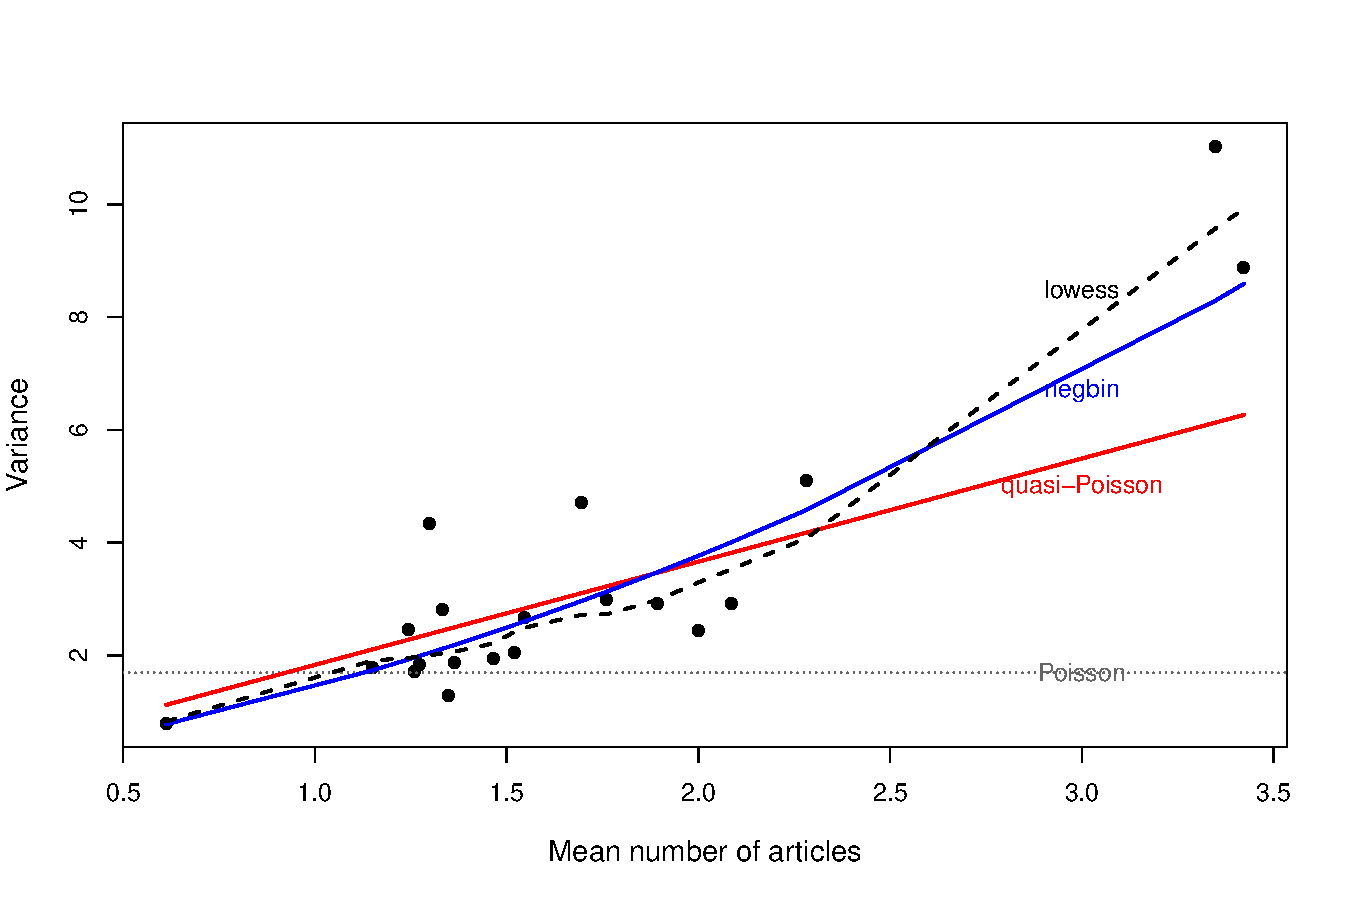
\includegraphics[width=.75\textwidth]{ch09/fig/phd-mean-var-plot-1} }

\caption[Mean--variance functions for the PhdPubs data]{Mean--variance functions for the PhdPubs data. Points show the observed means and variances for 20 quantile groups based on the fitted values in the negative-binomial model. The labeled lines and curves show the variance functions implied by various models.\label{fig:phd-mean-var-plot}}
\end{figure}


\end{knitrout}
We can see from this plot that the variances implied by the quasi-Poisson and negative-binomial
models are in reasonable accord with the data and with each other up to a mean of about 2.5.
They diverge substantially at the upper end, for the 20--30\% of the most productive
candidates, where the quadratic variance function of the negative-binomial provides a
better fit.

Finally, we can also compare the standard errors of coefficients
for the various methods designed to correct for overdispersion.  These are extracted
as the diagonal elements of the \func{vcov} and \func{sandwich} methods from the model objects.
\begin{knitrout}
\definecolor{shadecolor}{rgb}{1, 0.961, 0.933}\color{fgcolor}\begin{kframe}
\begin{alltt}
\hlkwd{library}\hlstd{(sandwich)}
\hlstd{phd.SE} \hlkwb{<-} \hlkwd{sqrt}\hlstd{(}\hlkwd{cbind}\hlstd{(}
  \hlkwc{pois}\hlstd{=}\hlkwd{diag}\hlstd{(}\hlkwd{vcov}\hlstd{(phd.pois)),}
  \hlkwc{sand}\hlstd{=}\hlkwd{diag}\hlstd{(}\hlkwd{sandwich}\hlstd{(phd.pois)),}
  \hlkwc{qpois}\hlstd{=}\hlkwd{diag}\hlstd{(}\hlkwd{vcov}\hlstd{(phd.qpois)),}
  \hlkwc{nbin}\hlstd{=}\hlkwd{diag}\hlstd{(}\hlkwd{vcov}\hlstd{(phd.nbin))))}
\hlkwd{round}\hlstd{(phd.SE,}\hlnum{4}\hlstd{)}
\end{alltt}
\begin{verbatim}
##               pois   sand  qpois   nbin
## (Intercept) 0.0996 0.1382 0.1348 0.1327
## female1     0.0546 0.0714 0.0738 0.0726
## married1    0.0613 0.0823 0.0829 0.0819
## kid5        0.0401 0.0560 0.0543 0.0528
## phdprestige 0.0253 0.0392 0.0342 0.0343
## mentor      0.0020 0.0039 0.0027 0.0032
\end{verbatim}
\end{kframe}
\end{knitrout}
For this example, the sandwich, quasi-Poisson and negative-binomial methods give similar results,
all about 40\% larger on average than those from the Poisson model.
\end{Example}

\subsection{Testing overdispersion}\label{sec:glm-disptest}

The forms of overdispersion seen in these examples and in \figref{fig:phd-mean-var-plot}
give rise to a statistical test
(\citealt{CameronTrivedi:1990}; \citealt[\S 3.4]{CameronTrivedi:1998})
for the
null hypothesis of Poisson variation, $H_0 : \V(y) = \mu$ against an alternative that the variance
has a particular form depending on the mean,
\begin{equation*}
\V(y) = \mu + \alpha \times f(\mu) \comma
\end{equation*}
where $f(\mu)$ is a given transformation function of the mean.

Overdispersion corresponds to $\alpha > 0$ and underdispersion to $\alpha < 0$.
The coefficient $\alpha$ can be estimated by an auxiliary OLS regression (without an intercept, i.e., of the
form
\begin{verbatim}
lm(var ~ -1 + f(mean)
\end{verbatim}
and tested with the corresponding $t$ (or $z$) statistic, which is asymptotically standard normal under the null hypothesis.

Common specifications of the transformation function are  $f(\mu) = \mu$ and $f(\mu) = \mu^2$. The first corresponds to
a NB model with a linear variance function (called NB1 by various authors)
or a quasi-Poisson model with dispersion parameter $\phi$, i.e.,
\begin{equation*}
\V(y) = (1 + \alpha) \mu = \phi \mu \period
\end{equation*}
The second is the more traditional form with quadratic variance function described in \secref{sec:glm-negbin}
(called NB2 by some authors).

These tests are carried out using the \func{dispersiontest} function in the \Rpackage{AER}.
The first argument is a Poisson GLM model; the second specifies the alternative hypothesis,
either as an integer power of $\mu$ or a function of the mean.
\begin{knitrout}
\definecolor{shadecolor}{rgb}{1, 0.961, 0.933}\color{fgcolor}\begin{kframe}
\begin{alltt}
\hlkwd{library}\hlstd{(AER)}
\hlkwd{dispersiontest}\hlstd{(phd.pois)}
\end{alltt}
\begin{verbatim}
## 
## 	Overdispersion test
## 
## data:  phd.pois
## z = 5.7347, p-value = 4.885e-09
## alternative hypothesis: true dispersion is greater than 1
## sample estimates:
## dispersion 
##     1.8259
\end{verbatim}
\begin{alltt}
\hlkwd{dispersiontest}\hlstd{(phd.pois,} \hlnum{2}\hlstd{)}
\end{alltt}
\begin{verbatim}
## 
## 	Overdispersion test
## 
## data:  phd.pois
## z = 6.4579, p-value = 5.308e-11
## alternative hypothesis: true alpha is greater than 0
## sample estimates:
##   alpha 
## 0.50877
\end{verbatim}
\end{kframe}
\end{knitrout}
These tests use a specified alternative hypothesis, so there is no way to compare directly which of
the NB1 or NB2 models is better or worse, except by using methods such as
AIC or BIC described in \secref{sec:glm-nonnest}.


\subsection{Visualizing goodness-of-fit}\label{sec:glm-visfit}

Even with correction for overdispersion, goodness-of-fit tests provide only an overall
summary of model fit.  Some specialized tests for particular forms of overdispersion
are also available (e.g., see \citet[\C 5]{CameronTrivedi:1998}),
but these only identify general problems and cannot provide detailed indications of
the possible source of these problems.

In \chref{ch:discrete}, we illustrated the use of rootograms for visualizing goodness-of-fit
to a wide variety discrete distributions using the \func{plot} method for
class \class{goodfit} objects with the \Rpackage{vcd}.  However, those methods were
developed for one-way discrete distributions without explanatory variables.

\citet{KleiberZeileis:2014} have generalized this idea to the wider class of
GLM-related count regression models considered here.
The \Rpackage{countreg} provides a new implementation of \func{rootogram}
with methods for all of these models (and others not mentioned).
We illustrate these plots for the models considered to this point, and then extend
this use for models allowing for excess zero counts in \secref{sec:glm-zeros}.

\begin{Example}[phdpubs4]{Publications of PhD candidates}
For the \data{PhdPubs} data, \figref{fig:phdpubs4-rootogram} shows hanging rootograms for the
Poisson and negative-binomial models produced using \code{countreg::rootogram}%
\footnote{
At the time of this writing, \code{rootogram} in \pkg{countreg} conflicts with
the version in \pkg{vcd}, so we qualify the use here with the package name.
}
on the fitted model objects.  We are looking both for general patterns of under/over fit, as well
as counts that stand out as poorly fitted against the background.

\begin{knitrout}
\definecolor{shadecolor}{rgb}{1, 0.961, 0.933}\color{fgcolor}\begin{kframe}
\begin{alltt}
\hlkwd{library}\hlstd{(countreg)}
\hlstd{countreg::}\hlkwd{rootogram}\hlstd{(phd.pois,} \hlkwc{max}\hlstd{=}\hlnum{12}\hlstd{,} \hlkwc{main}\hlstd{=}\hlstr{"PhDPubs: Poisson"}\hlstd{)}
\hlstd{countreg::}\hlkwd{rootogram}\hlstd{(phd.nbin,} \hlkwc{max}\hlstd{=}\hlnum{12}\hlstd{,} \hlkwc{main}\hlstd{=}\hlstr{"PhDPubs: Negative-Binomial"}\hlstd{)}
\end{alltt}
\end{kframe}\begin{figure}[!htbp]


\centerline{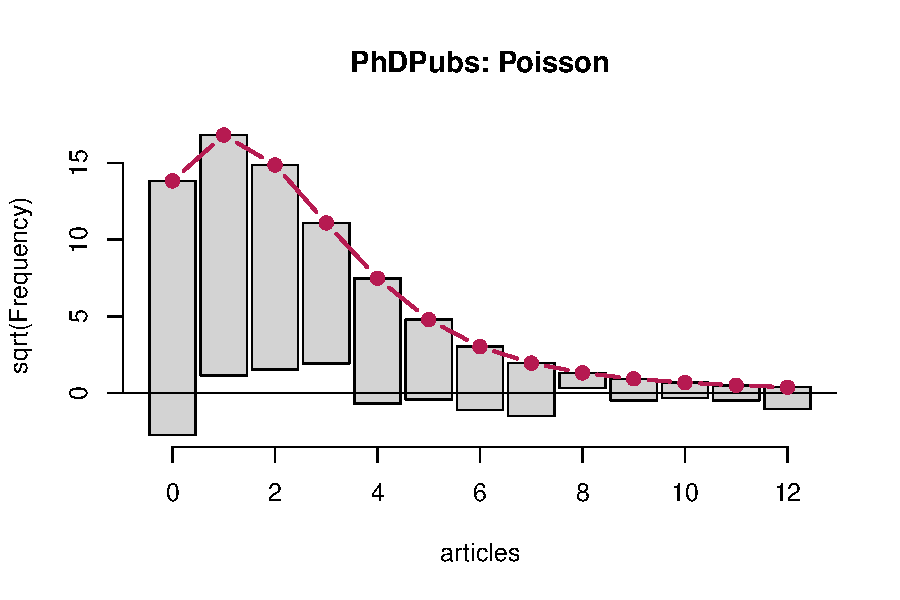
\includegraphics[width=.49\textwidth]{ch09/fig/phdpubs4-rootogram-1} 
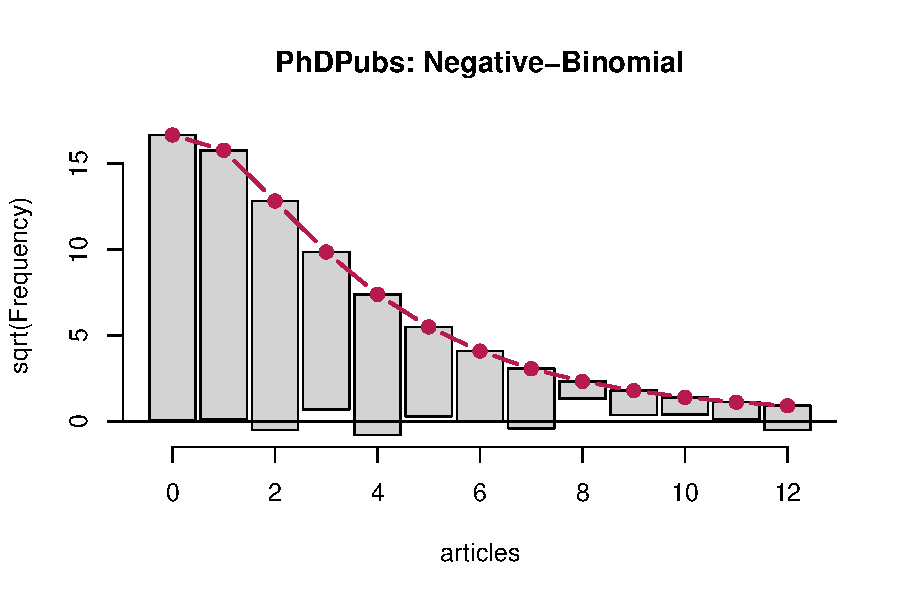
\includegraphics[width=.49\textwidth]{ch09/fig/phdpubs4-rootogram-2} }

\caption[Hanging rootograms for the PhdPubs data]{Hanging rootograms for the PhdPubs data.\label{fig:phdpubs4-rootogram}}
\end{figure}


\end{knitrout}
The Poisson model shows a systematic, wave-like pattern with excess zeros, too few observed frequencies for
counts of
1--3, but generally greater frequencies for counts of 4 or more.  The negative-binomial model
clearly fits much better, though there is a peculiar tendency among the smaller
frequencies for 8 or more articles.
\end{Example}

\begin{Example}[crabs2]{Mating of horseshoe crabs}
\figref{fig:crabs2-rootogram} shows similar plots for the same two models fit to the number of
crab satellites.  The fit of the Poisson model clearly reveals the excess of zero male satellites.
For the negative-binomial, the rootogram no longer exhibits same wave-like pattern,
however, the underfitting of the count for 0 and overfitting for counts 1--2 is
characteristic of data with excess zeros.

\begin{knitrout}
\definecolor{shadecolor}{rgb}{1, 0.961, 0.933}\color{fgcolor}\begin{kframe}
\begin{alltt}
\hlstd{countreg::}\hlkwd{rootogram}\hlstd{(crabs.pois,} \hlkwc{max}\hlstd{=}\hlnum{15}\hlstd{,} \hlkwc{main}\hlstd{=}\hlstr{"CrabSatellites: Poisson"}\hlstd{)}
\hlstd{countreg::}\hlkwd{rootogram}\hlstd{(crabs.nbin,} \hlkwc{max}\hlstd{=}\hlnum{15}\hlstd{,} \hlkwc{main}\hlstd{=}\hlstr{"CrabSatellites: Negative-Binomial"}\hlstd{)}
\end{alltt}
\end{kframe}\begin{figure}[!htbp]


\centerline{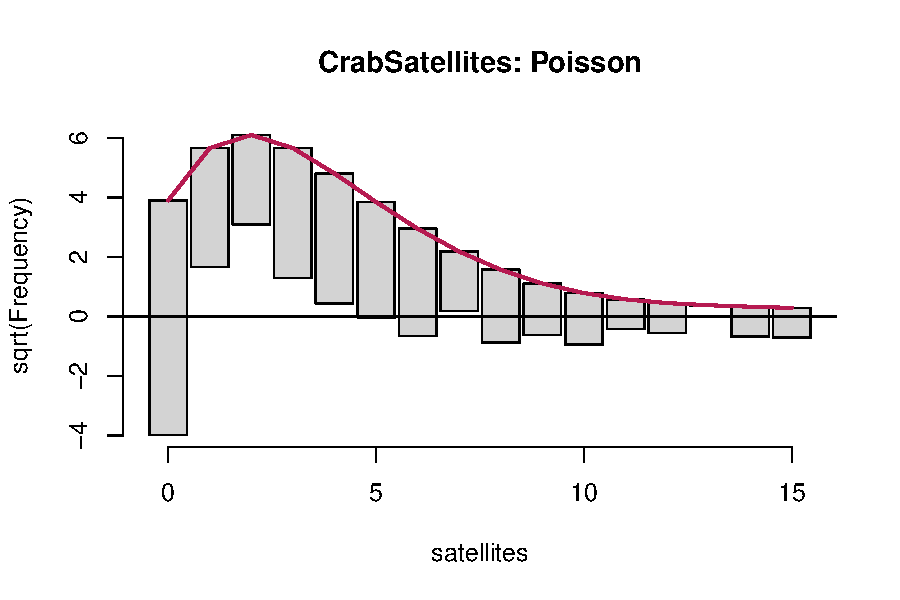
\includegraphics[width=.49\textwidth]{ch09/fig/crabs2-rootogram-1} 
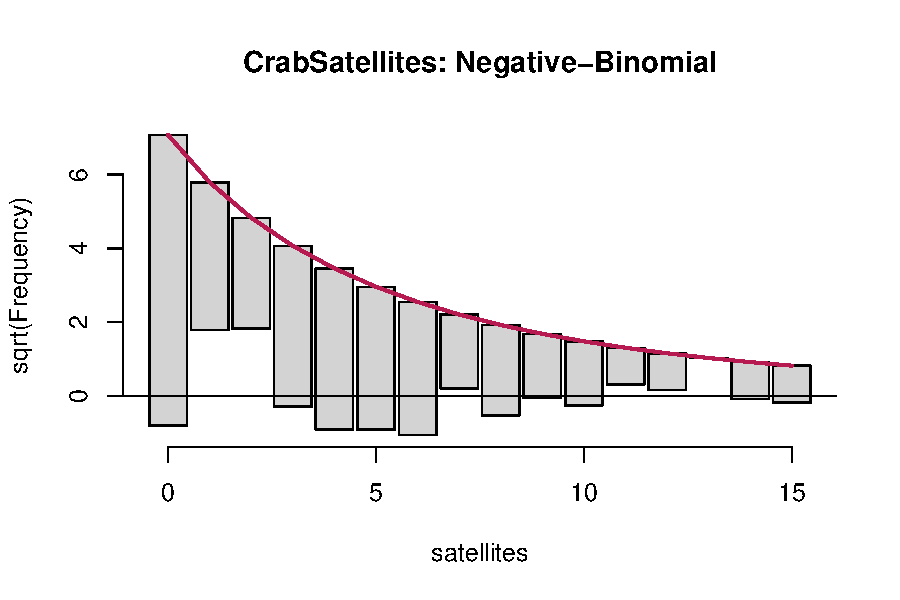
\includegraphics[width=.49\textwidth]{ch09/fig/crabs2-rootogram-2} }

\caption[Hanging rootograms for the CrabSatellites data]{Hanging rootograms for the CrabSatellites data.\label{fig:crabs2-rootogram}}
\end{figure}


\end{knitrout}
\end{Example}



\section{Models for excess zero counts}\label{sec:glm-zeros}

%\section{Models for excess zero counts}\label{sec:glm-zeros}

In addition to overdispersion, many sets of empirical data exhibit a greater prevalence of
zero counts than can be accommodated by the Poisson or negative-binomial models.
We saw this in the \data{PhdPubs} data set, where there were many candidates who had
not published at all, and in the \data{CrabSatellites} data where a large number of
females attracted no unattached males.
Other examples abound in many different fields: studies of the
use of health care services often find that many people never visit a hospital
in some time frame; similarly, the distribution of insurance claims often shows
large numbers who make no claims \citep{YipYau:2005} because of under-reporting
of small claims, policy deductible provisions and desire to avoid premium increases.


Beyond simply identifying this as a problem of lack-of-fit,
understanding the reasons for excess zero counts can make a contribution to a
more complete explanation of the phenomenon of interest,
and this requires both new statistical models and visualization techniques
illustrated in this section.

In the first example, \citet{Long:1997} argued that the PhD candidates might fall into
two distinct groups: ``publishers'' (perhaps striving for an academic career)
and ``non-publishers'' (seeking other career paths).  Of the 275 observations
having \code{articles==0}, some might not have published due to chance or
unmeasured factors.  One reasonable form of explanation is that the observed
zero counts reflect a mixture of the two latent classes--- those who simply
have not yet published and those who will likely never publish.
A statistical formulation of this idea leads to the class of \emph{zero-inflated}
models described below.

A different form of explanation is that there may be some special
circumstance or ``hurdle'' required to achieve a positive count,
like publishing the master's thesis
(such as being driven internally by a personality trait or externally by
pressure from a mentor). This idea leads to the class of \emph{hurdle} models
that entertain and fit (simultaneously) two separate models: one for the
occurrence of the zero counts, and one for the positive counts.
These two approaches are illustrated in \figref{fig:ExcessZeros}

\begin{figure}[htb]
  \centering
  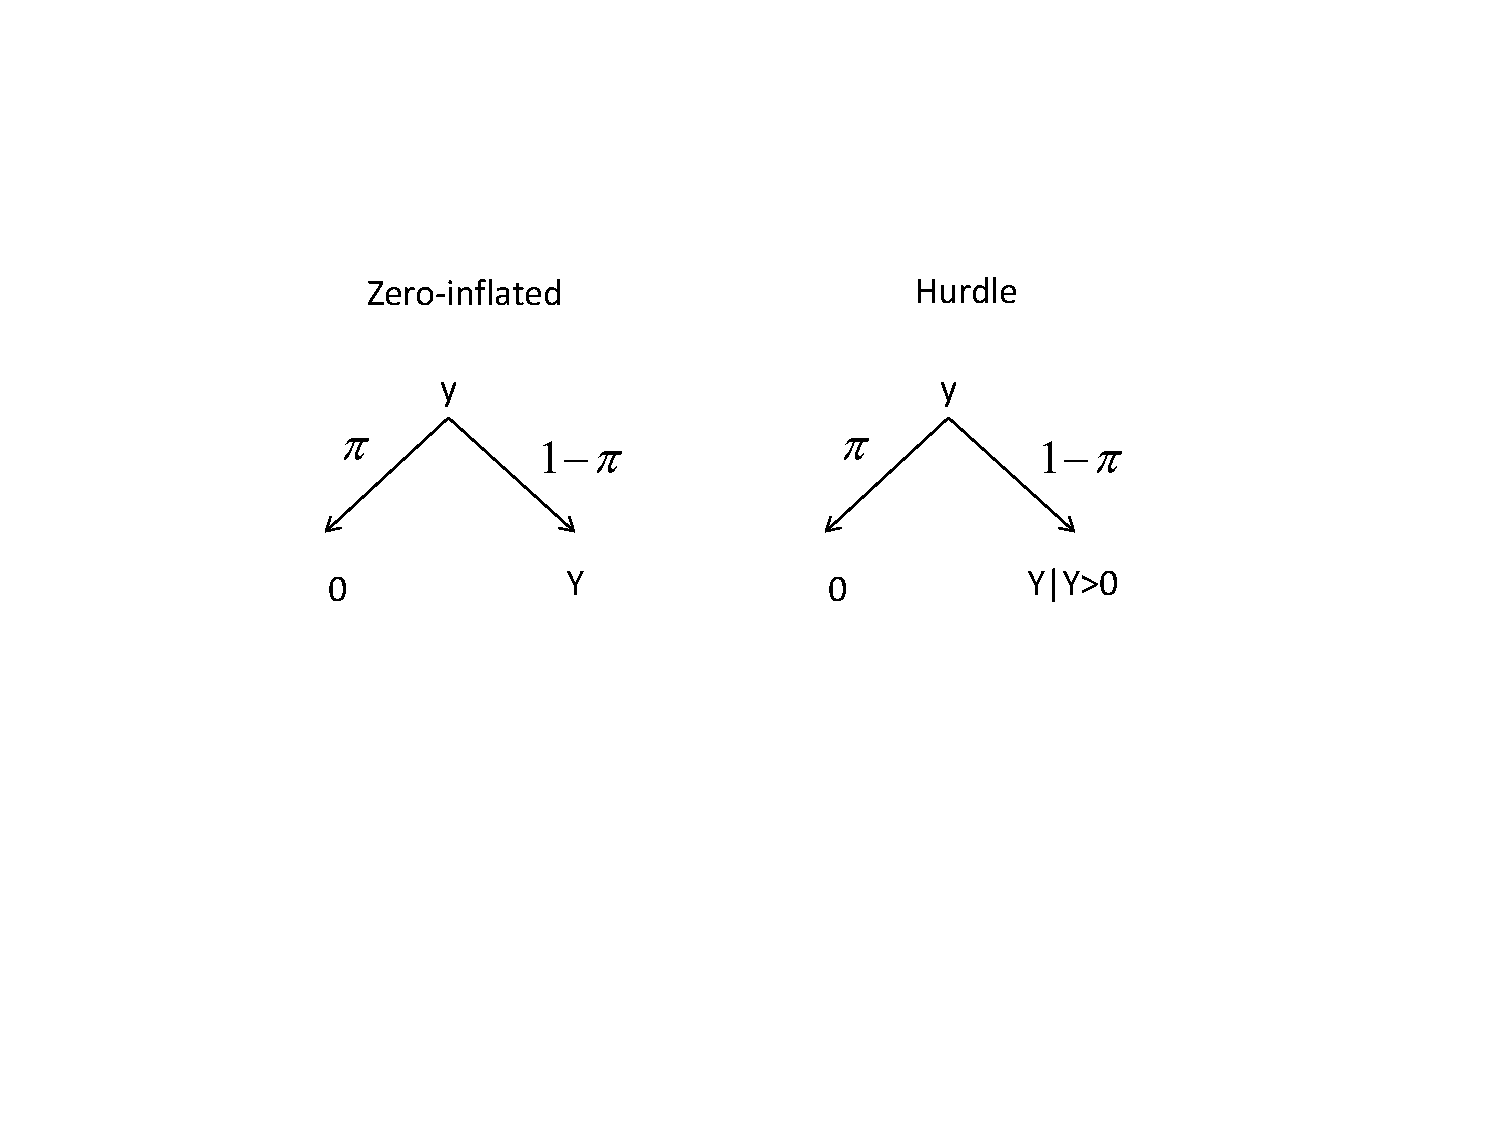
\includegraphics[width=.6\textwidth]{ch09/fig/ExcessZeros}
  \caption{Models for excess zeros. The observed response $y$ is derived from a latent or parent
  distribution for $Y$ yielding zero counts with probability $\pi$.}
  \label{fig:ExcessZeros}
\end{figure}

\subsection{Zero-inflated models}\label{sec:glm-zip}

Zero-inflated models, introduced by \citet{Lambert:1992} as the \term{zero-inflated Poisson}
(ZIP) model, provide an attractive solution to the problem of dealing with an overabundance of
zero counts.  It postulates that the observed counts arise from a mixture of two latent classes
of observations: some structural zeros for whom $y_i$ will always be 0, and the rest, sometimes
giving random zeros.
The ZIP model is comprised of two components:
\begin{itemize}
  \item A model for the binary event of membership in the unobserved (latent) class of
  those for whom the count is necessarily zero (e.g., ``non-publishers'').
  This is typically taken as a logistic regression for the probability $\pi_i$ that
  observation $i$ is in this class, with predictors $\vec{z}_1, \vec{z}_2, \dots, \vec{z}_q$, giving
\begin{equation}\label{eq:zip-logit}
 \logit (\pi_i) = \vec{z}_i\trans \vec{\gamma}
                = \gamma_0 + \gamma_1 z_{i1} + \gamma_2 z_{i2} + \cdots + \gamma_q z_{iq} \period
\end{equation}

  \item A Poisson model for the other class (e.g., ``publishers''), for whom the observed count may 0 or
  positive. This model typically uses the usual log link to predict the mean, using predictors
  $\vec{x}_1, \vec{x}_2, \dots, \vec{x}_p$, so
\begin{equation}\label{eq:zip-pois}
  \log_e  \: \mu (\vec{x}_i) = \vec{x}_i \trans \vec{\beta}
                 = \beta_0 + \beta_1 x_{i1} + \beta_2 x_{i2} + \cdots + \beta_q x_{ip} \period
\end{equation}
\end{itemize}
In application, it is permissible and not uncommon to use the same set of predictors
$x = z$ in both submodels, but the notation indicates that this is not required.
Some simple special cases arise when the model for the always zero latent class
is an intercept-only model, $\logit (\pi_i) = \gamma_0$, implying the same probability
for all individuals, and (less commonly) when the Poisson mean model is intercept-only
with no predictors but there might be excess zero counts.

With this setup, one can show that the probability of observing counts of $y_i = 0$
and $y_i > 0$ are
\begin{eqnarray}
\Pr ({y_i} = 0 \given \vec{x}, \vec{z}) &=& {\pi _i} + (1 - {\pi _i}){e^{ - {\mu _i}}} \label{eq:zip-probs} \\
\Pr ({y_i} \given \vec{x}, \vec{z}) &=& (1 - {\pi _i}) \times \left[\frac{{{\mu _i}^{{y_i}}{e^{ - {\mu _i}}}}}{{{y_i}!}} \right] \comma \quad\quad y_i \ge 0 \nonumber
\end{eqnarray}
where the term in brackets in the second equation is the Poisson probability $\Pr(y=y_i)$
with rate parameter $\Pois(\mu_i)$. In these equations,
$\pi_i= \logit^{-1} (\vec{z}_i\trans \vec{\gamma}) $ depends on the $\vec{z}$ through \eqref{eq:zip-logit}, and
$\mu_i = \exp(\vec{x}\trans\vec{\beta})$ depends on the $\vec{x}$
through \eqref{eq:zip-pois}.

The conditional expectation and variance of $y_i$ then have the forms
\begin{eqnarray*}
\E (y_i) &=& (1 - {\pi _i}) \: \mu_i  \\
\V (y_i) &=& (1 - {\pi _i}) \: \mu_i  (1 + \mu_i \pi_i ) \period
\end{eqnarray*}
Thus, when $\pi_i > 0$, the mean of $y$ is always less than $\mu_i$,
and the variance of $y$ is greater than its mean by a dispersion factor of $(1 + \mu_i \pi_i)$.

There is nothing special about the use of the Poisson distribution here. The model for the
count variable could also be taken as the negative-binomial, giving a
\emph{zero-inflated negative-binomial} (ZINB) model using $\NBin (\mu, \theta)$ or
a \emph{zero-inflated geometric} model using $\NBin (\mu, \theta=1)$.

\begin{Example}[zipois]{Simulating zero-inflated data}

A simple way of understanding the effects of zero-inflation on count data is
to simulate data from their distribution and plot it.  For the
standard Poisson and negative-binomial, random values can be generated using
\func{rpois} and \func{rnegbin} (in \pkg{MASS}), respectively.
Their zero-inflated counterparts are implemented in the \Rpackage{VGAM}
as \func{rzipois} and \func{rzinegbin}.

To illustrate this use, we generate two random data sets using \func{rzipois}
having constant mean $\mu=3$.  The first is a standard Poisson ($\pi=0$),
while the second has a constant probability $\pi=0.3$ of an excess zero.

\begin{knitrout}
\definecolor{shadecolor}{rgb}{1, 0.961, 0.933}\color{fgcolor}\begin{kframe}
\begin{alltt}
\hlkwd{library}\hlstd{(VGAM)}
\hlkwd{set.seed}\hlstd{(}\hlnum{1234}\hlstd{)}
\hlstd{data1} \hlkwb{<-} \hlkwd{rzipois}\hlstd{(}\hlnum{200}\hlstd{,} \hlnum{3}\hlstd{,} \hlnum{0}\hlstd{)}
\hlstd{data2} \hlkwb{<-} \hlkwd{rzipois}\hlstd{(}\hlnum{200}\hlstd{,} \hlnum{3}\hlstd{,} \hlnum{.3}\hlstd{)}
\end{alltt}
\end{kframe}
\end{knitrout}
Barplots of the frequencies in these data sets are shown in \figref{fig:zipois-plot}.
The sample mean in \code{data1} is 2.925, quite close to $\mu=3$.
In the zero-inflated \code{data2}, the mean is only 2.25 due to the excess zeros.
\begin{knitrout}
\definecolor{shadecolor}{rgb}{1, 0.961, 0.933}\color{fgcolor}\begin{kframe}
\begin{alltt}
\hlstd{tdata1} \hlkwb{<-} \hlkwd{table}\hlstd{(data1)}
\hlkwd{barplot}\hlstd{(tdata1,} \hlkwc{xlab}\hlstd{=}\hlstr{"Count"}\hlstd{,} \hlkwc{ylab}\hlstd{=}\hlstr{"Frequency"}\hlstd{,}
        \hlkwc{main}\hlstd{=}\hlstr{"Poisson(3)"}\hlstd{)}
\hlstd{tdata2} \hlkwb{<-} \hlkwd{table}\hlstd{(data2)}
\hlkwd{barplot}\hlstd{(tdata2,} \hlkwc{xlab}\hlstd{=}\hlstr{"Count"}\hlstd{,} \hlkwc{ylab}\hlstd{=}\hlstr{"Frequency"}\hlstd{,}
        \hlkwc{main}\hlstd{=}\hlkwd{expression}\hlstd{(}\hlstr{"ZI Poisson(3, "} \hlopt{*} \hlstd{pi} \hlopt{*} \hlstr{"= .3)"}\hlstd{))}
\end{alltt}
\end{kframe}\begin{figure}[!htbp]


\centerline{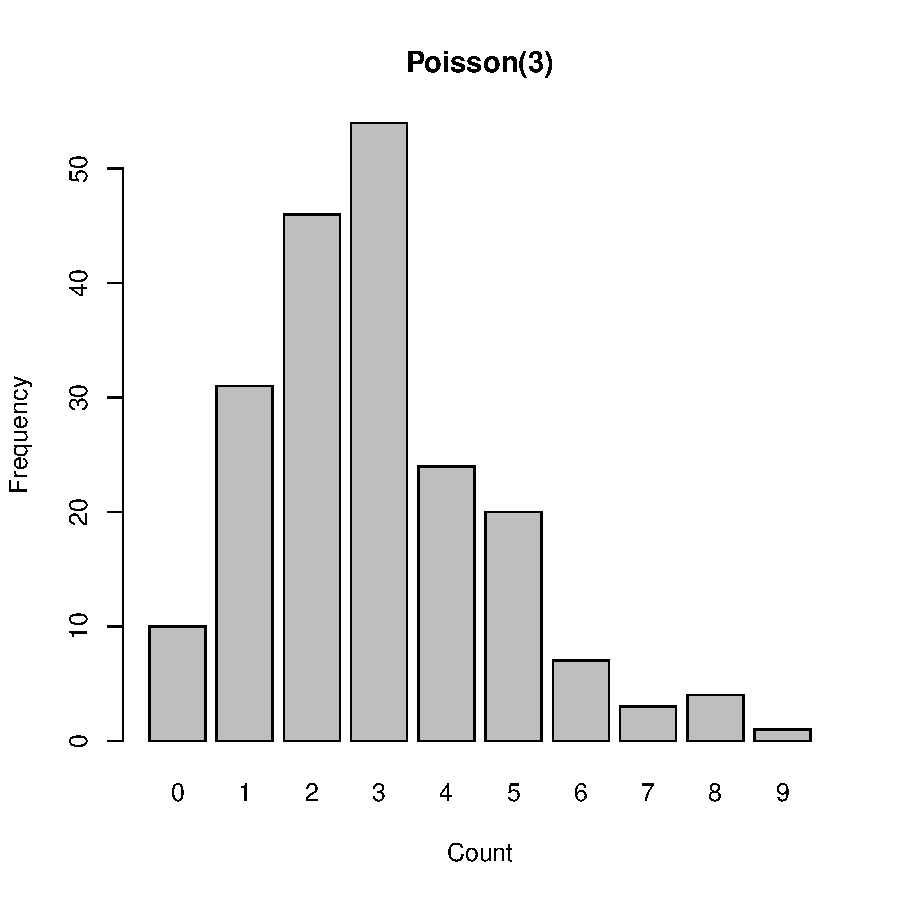
\includegraphics[width=.49\textwidth]{ch09/fig/zipois-plot-1} 
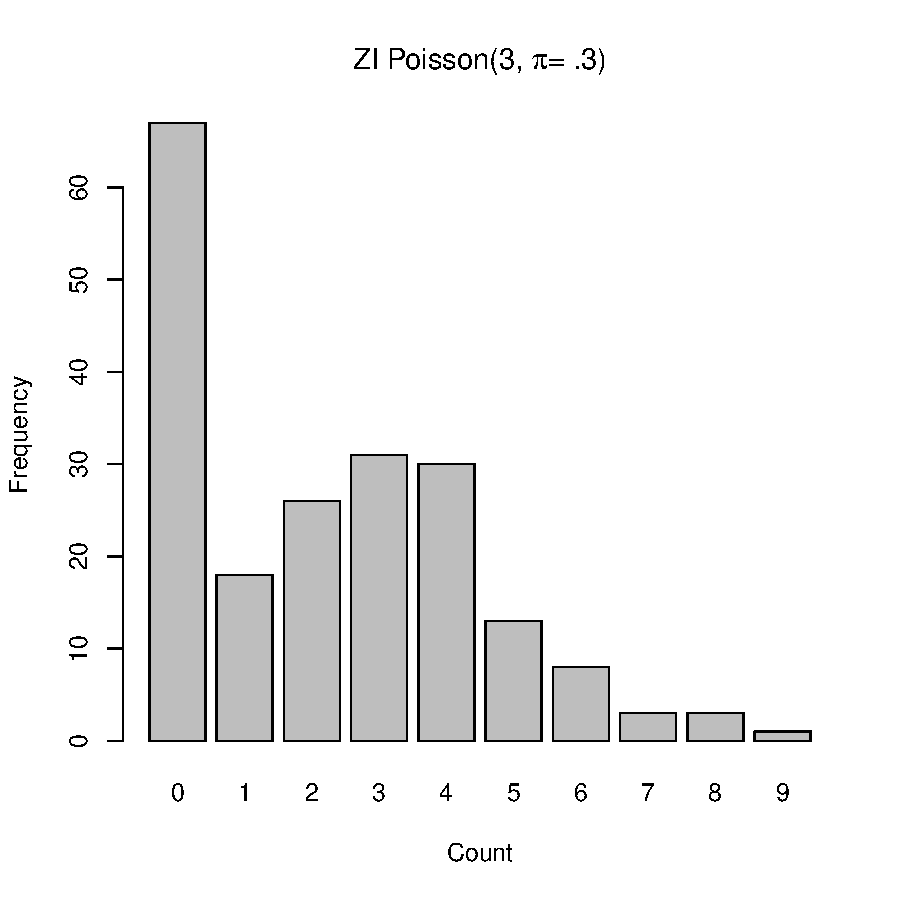
\includegraphics[width=.49\textwidth]{ch09/fig/zipois-plot-2} }

\caption[Bar plots of simulated data from Poisson and zero-inflated Poisson distributions]{Bar plots of simulated data from Poisson and zero-inflated Poisson distributions\label{fig:zipois-plot}}
\end{figure}


\end{knitrout}



\end{Example}

There are several packages in \R capable of fitting zero-inflated models.  The most mature and
complete of these is \func{zeroinfl} in
the \Rpackage{countreg} (a successor to the \Rpackage{pscl})
The function \func{zeroinfl} is modeled after \func{glm}, but provides an extended syntax
for the model formula.

If the \code{formula} argument is supplied in the form
\verb|y ~ x1 + x2 + ...|, it not only describes the count regression of $y$ on
$x_1, x_2, \dots$, but also implies that the \emph{same} set of regressors, $z_j = x_j$,
is used for the zero count binary submodel.  The extended syntax  uses the
notation
\verb#y ~ x1 + x2 + ... | z1 + z2 + ...#
to specify the $x$ variables separately, conditional on (\code{|})
the always-zero count model \verb|y ~ z1 + z2 + ...|.
The model for the not-always-zero class can be specified using the
\code{dist} argument, with possible values
\code{"poisson"}, \code{"negbin"} and \code{"geometric"}.


\subsection{Hurdle models}\label{sec:glm-hurdle}
A different class of models capable of accounting for excess zero counts is the
\term{hurdle model} (also called the \term{zero-altered model})
proposed initially by \citet{Cragg:1971} and developed further by
\citet{Mullahy:1986}.
This model also uses a separate logistic regression submodel to distinguish
counts of $y=0$ from larger counts, $y>0$.
The submodel for the positive counts is expressed as a (left) \emph{truncated}
Poisson or negative-binomial model, excluding the zero counts.
As an example, consider a study of behavioral health in which one outcome is
the number of cigarettes smoked in one month.  All the zero counts will come from
non-smokers and smokers will nearly always smoke a positive number.

This differs from the set of ZIP models in that classes of $y=0$ and $y>0$
are now considered fully-observed, rather than latent.
Conceptually, there is one process and submodel accounting for the zero counts
and a separate process accounting for the positive counts, once the ``hurdle''
of $y=0$ has been passed.
In other words, for ZIP models, the first process generates
only extra zeros beyond those of the regular Poisson distribution.
For hurdle models, the first process generates all of the zeros.
The probability equations corresponding to \eqref{eq:zip-probs} are:
\begin{eqnarray}
\Pr ({y_i} = 0 \given \vec{x}, \vec{z}) &=& {\pi _i} \\
\Pr ({y_i} \given \vec{x}, \vec{z}) &=& \frac{(1 - {\pi _i})}{1-e^{-\mu_i}}
\times \left[\frac{{{\mu _i}^{{y_i}}{e^{ - {\mu _i}}}}}{{{y_i}!}} \right] \comma \quad\quad y_i \ge 0 \nonumber
\end{eqnarray}
% and the mean regression relationship can be expressed as
% \begin{equation*}
%  \log_e  \: \mu (\vec{x}_i) = \vec{x}_i \trans \vec{\beta}
%           + log_e (1 - \pi_i) - log_e(1 - )
% \end{equation*}

The hurdle model can be fitted in \R using the \func{hurdle} function from the \Rpackage{countreg}.
The syntax for the model formula is the same extended form provided by \func{zeroinfl},
where \verb|y ~ x1 + x2| uses the same regressors for the zero and positive count submodels,
while \verb#y ~ x1 + x2 | z1 + z2# uses \verb|y ~ z1 + z2| for the zero hurdle model.
Similarly, the count distribution can be given
as
\code{"poisson"}, \code{"negbin"} or \code{"geometric"}
with the \code{dist} argument.  For \func{hurdle}, the distribution for zero model
can be specified with a \code{zero.dist} argument. The default is \code{"binomial"}
(with a logit \code{link}), but other right-censored
distributions can also be specified.

\subsection{Visualizing zero counts}\label{sec:glm-viszero}

Both the zero-inflated and hurdle models treat the zero counts $y=0$ specially with separate
submodels, so the binary event of $y=0$ vs.\ $y>0$ can be visualized using any of the techniques
illustrated in \chref{ch:logistic}.  See \secref{sec:logist-plotting}, \secref{sec:logist-condplots}
and \secref{sec:logist-fullplots} for some examples that plot both the binary observations
and a model summary or smoothed curve to show the relationships with one or more
regressors.  To apply these ideas in the current context, simply define or plot a logical
variable corresponding to the expression \code{y==0}, giving values of \code{TRUE} or \code{FALSE}.

A different, and simpler idea is illustrated here using what is called a \term{spine plot}
\cite{Hummel:96} when a predictor $x$ is a discrete factor or \term{spinogram} when $x$ is
continuous.  Both are forms of mosaic plots with special formatting of spacing and shading,
and in this context they plot $\Pr(y=0 | x)$ against $\Pr(x)$; when $x$ is numerical, it
is first made discrete, as in a histogram.
Then, in the spine plot or spinogram, the widths of the bars correspond to the relative frequencies of $x$
and heights of the bars correspond to the conditional relative frequencies of $y=0$ in every $x$ group.
In \R, spine plots are implemented in the function \func{spineplot}, however, this is what you
get by default if you use \verb|plot(y==0 ~ x)| to plot the binary factor against any regressor $x$.

A related graphical method is the \term{conditional density plot}
\citep{HofmannTheus:2005}. The conditional probabilities $\Pr(y=0 | x)$ are derived using
a smoothing approach (via \func{density}) over $x$ rather than by making $x$ discrete.
These plots are provided by \func{cdplot} in the \Rpackage{graphics} and a similar
\func{cd\_plot} in \pkg{vcd}.  The smoothing method for the density estimate is controlled
by a \code{bw} (bandwidth) method and other arguments.

\begin{Example}[crabs-zero]{Mating of horseshoe crabs}
For the \data{CrabSatellites} data, we can examine the relationship of the zero counts
(females who attract no unattached male satellites) to the predictors using spinograms
or conditional density plots.  Here, we consider \var{weight} and \var{color} (treated numerically) as
predictors. \TODO{Fixup use of color in \exref{ex:crabs1} so it doesn't cause a problem here}


Spinograms for the occurrence of zero satellites
against \var{weight} and \var{color} are shown in \figref{fig:crabs-zero-spinogram},
where we have used quantiles of those distributions to define the breaks on the
horizontal axis. Using \code{ylevels=2:1} reverses the order of the vertical
categories.
You can easily see that the zeros decrease steadily with
weight and increase with darkness.

\begin{knitrout}
\definecolor{shadecolor}{rgb}{1, 0.961, 0.933}\color{fgcolor}\begin{kframe}
\begin{alltt}
\hlstd{op} \hlkwb{<-} \hlkwd{par}\hlstd{(}\hlkwc{cex.lab}\hlstd{=}\hlnum{1.2}\hlstd{,} \hlkwc{mfrow} \hlstd{=} \hlkwd{c}\hlstd{(}\hlnum{1}\hlstd{,} \hlnum{2}\hlstd{))}
\hlkwd{plot}\hlstd{(}\hlkwd{factor}\hlstd{(satellites} \hlopt{==} \hlnum{0}\hlstd{)} \hlopt{~} \hlstd{weight,} \hlkwc{data} \hlstd{= CrabSatellites,}
     \hlkwc{breaks} \hlstd{=} \hlkwd{quantile}\hlstd{(weight,} \hlkwc{probs}\hlstd{=}\hlkwd{seq}\hlstd{(}\hlnum{0}\hlstd{,}\hlnum{1}\hlstd{,}\hlnum{.2}\hlstd{)),} \hlkwc{ylevels}\hlstd{=}\hlnum{2}\hlopt{:}\hlnum{1}\hlstd{,}
     \hlkwc{ylab}\hlstd{=}\hlstr{"No satellites"}\hlstd{)}
\hlkwd{plot}\hlstd{(}\hlkwd{factor}\hlstd{(satellites} \hlopt{==} \hlnum{0}\hlstd{)} \hlopt{~} \hlstd{color,} \hlkwc{data} \hlstd{= CrabSatellites,}
     \hlkwc{breaks} \hlstd{=} \hlkwd{quantile}\hlstd{(color,} \hlkwc{probs}\hlstd{=}\hlkwd{seq}\hlstd{(}\hlnum{0}\hlstd{,}\hlnum{1}\hlstd{,}\hlnum{.33}\hlstd{)),}  \hlkwc{ylevels}\hlstd{=}\hlnum{2}\hlopt{:}\hlnum{1}\hlstd{,}
     \hlkwc{ylab}\hlstd{=}\hlstr{"No satellites"}\hlstd{)}
\hlkwd{par}\hlstd{(op)}
\end{alltt}
\end{kframe}\begin{figure}[!htbp]


\centerline{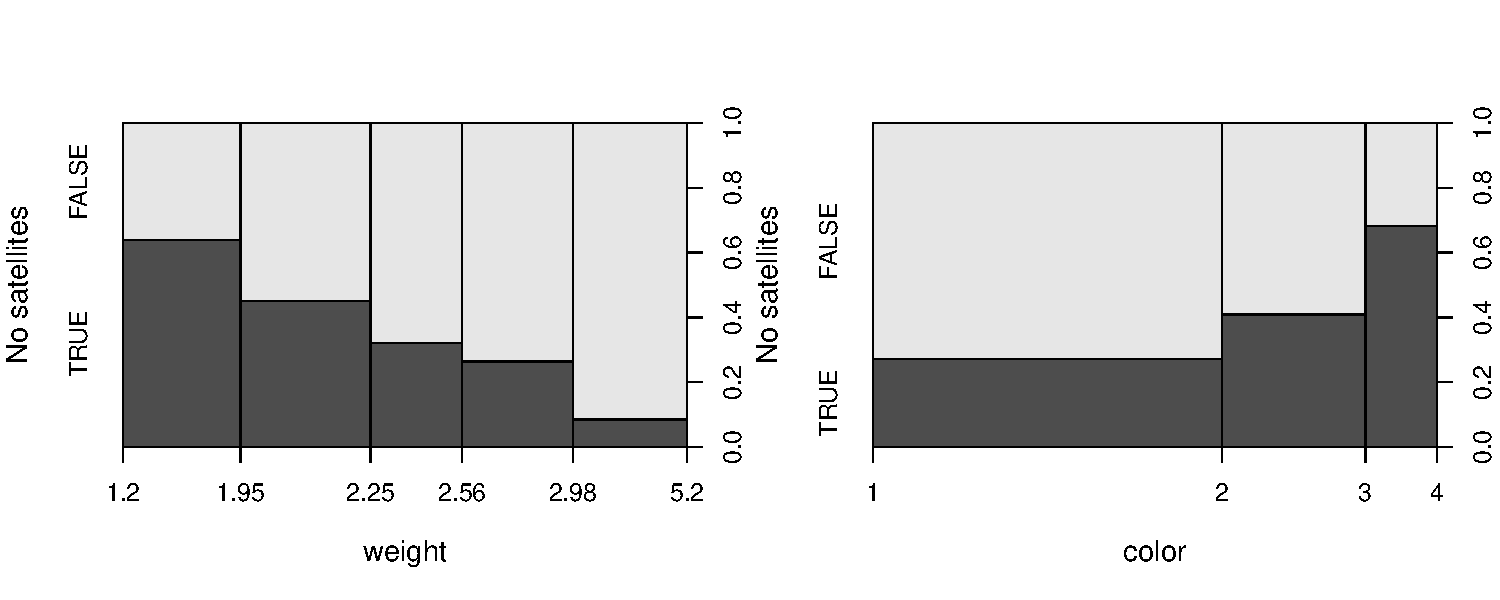
\includegraphics[width=\textwidth]{ch09/fig/crabs-zero-spinogram-1} }

\caption[Spinograms for the CrabSatellites data]{Spinograms for the CrabSatellites data. The variables weight (left) and color(right) have been made discrete using quantiles of their distributions.\label{fig:crabs-zero-spinogram}}
\end{figure}


\end{knitrout}

Similar plots in the form of conditional density plots are shown in
\figref{fig:crabs-zero-cdplot}, with a similar interpretation.
\begin{knitrout}
\definecolor{shadecolor}{rgb}{1, 0.961, 0.933}\color{fgcolor}\begin{kframe}
\begin{alltt}
\hlstd{op} \hlkwb{<-} \hlkwd{par}\hlstd{(}\hlkwc{cex.lab}\hlstd{=}\hlnum{1.2}\hlstd{,} \hlkwc{mfrow} \hlstd{=} \hlkwd{c}\hlstd{(}\hlnum{1}\hlstd{,} \hlnum{2}\hlstd{))}
\hlkwd{cdplot}\hlstd{(}\hlkwd{factor}\hlstd{(satellites} \hlopt{==} \hlnum{0}\hlstd{)} \hlopt{~} \hlstd{weight,} \hlkwc{data} \hlstd{= CrabSatellites,}
       \hlkwc{ylevels}\hlstd{=}\hlnum{2}\hlopt{:}\hlnum{1}\hlstd{,} \hlkwc{ylab}\hlstd{=}\hlstr{"No satellites"}\hlstd{)}
\hlkwd{cdplot}\hlstd{(}\hlkwd{factor}\hlstd{(satellites} \hlopt{==} \hlnum{0}\hlstd{)} \hlopt{~} \hlstd{color,} \hlkwc{data} \hlstd{= CrabSatellites,}
       \hlkwc{ylevels}\hlstd{=}\hlnum{2}\hlopt{:}\hlnum{1}\hlstd{, ,} \hlkwc{ylab}\hlstd{=}\hlstr{"No satellites"}\hlstd{)}
\hlkwd{par}\hlstd{(op)}
\end{alltt}
\end{kframe}\begin{figure}[!htbp]


\centerline{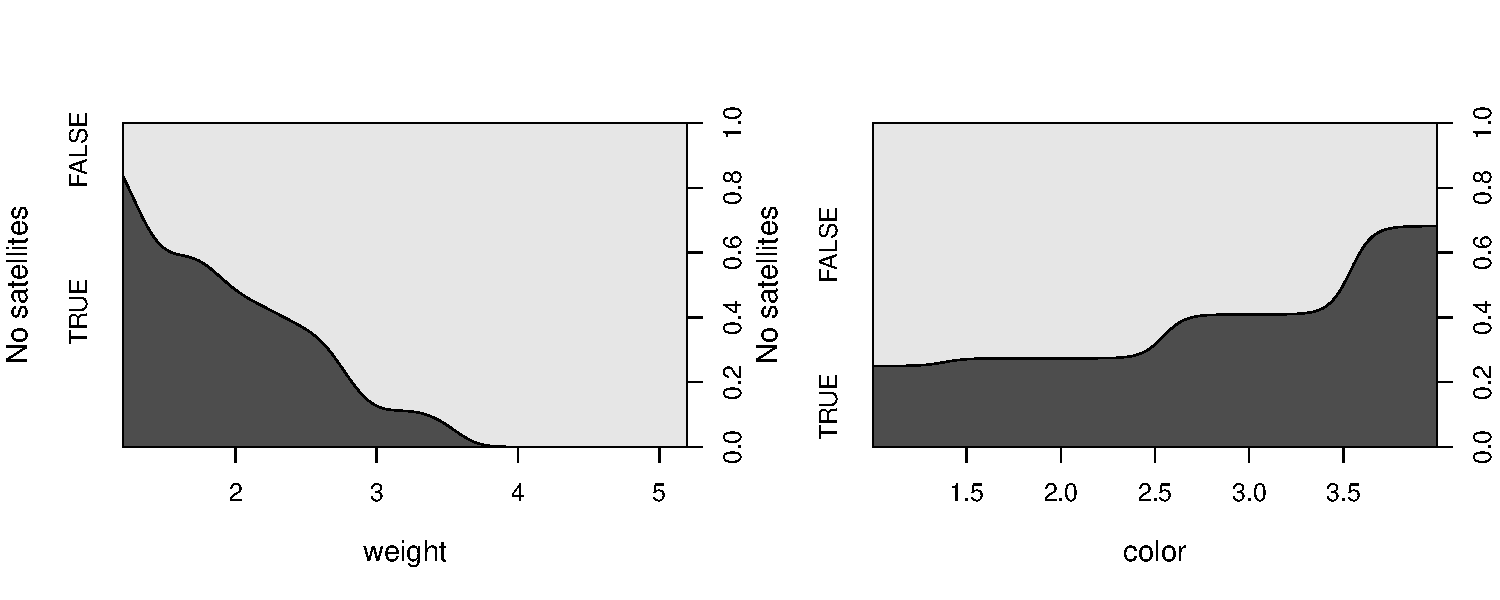
\includegraphics[width=\textwidth]{ch09/fig/crabs-zero-cdplot-1} }

\caption[Conditional density plots for the CrabSatellites data]{Conditional density plots for the CrabSatellites data. The region shaded below shows the conditional probability density estimate for a count of zero.\label{fig:crabs-zero-cdplot}}
\end{figure}


\end{knitrout}

\end{Example}

%\subsection{Zero-inflated models}\label{sec:glm-zip}
%\subsection{Hurdle models}\label{sec:glm-hurdle}

\section{Case studies}\label{sec:glm-casestudies}
In this section, we introduce two extended examples, designed to illustrate aspects of
exploratory analysis, visualization, model fitting, and interpretation for count data GLMs.
The first (\secref{sec:glm-case-cod})
concerns another well-known data set from ethology, where
\begin{seriate}
\item excess zeros require special treatment,
\item the occurrence of zero counts has substantive meaning, and
\item an interaction between two factors is important.
\end{seriate}

The second case study (\secref{sec:glm-case-nmes})
uses a larger, also well-known
data set from health economics, with more predictors and more
potential interactions. The emphasis shifts here from fitting and comparing models with
different distributional forms and link functions to selecting terms for an adequate descriptive
and explanatory model. Another feature of these examples is that the relatively large sample size
in this data supports a wider range of model complexity than is available in smaller samples.


\subsection{Cod parasites}\label{sec:glm-case-cod}
The cod fishery is extremely important to the economy of Norway, so anything that affects the
health of the cod population and its ecosystem can have severe consequences.
The red king crab \emph{Paralithodes camtschaticus} was deliberately introduced by Russian scientists
to the Barents Sea in the 1960s and 1970s from its native area in the North Pacific. The carapace of these crabs is used by the leech \emph{Johanssonia arctica} to deposit its eggs. This leech in turn is a vector for the blood parasite
\emph{Trypanosoma murmanensis} that can infect marine fish, including cod.


\citet{Hemmingsen-etal:2005} examined cod for trypanosome infections during annual cruises along the coast of Finnmark in North Norway over three successive years and in four different areas
(A1: S{\o}r{\o}ya; A2: Mager{\o}ya; A3: Tanafjord; A4: Varangerfjord).
They show that trypanosome infections are strongest in the area Varangerfjord where the density of red king crabs is highest. Thus, there is evidence that the introduction of the foreign red king crabs had an indirect detrimental effect on the health of the native cod population. This situation stands out because it is not an introduced \emph{parasite} that is dangerous for a native host, but rather an introduced \emph{host} that promotes transmission of two endemic parasites. They call the connections among these factors ``an unholy trinity.''%
\footnote{\label{fn:russian}
The four areas A1--A4 are arranged from east to west, with Varangerfjord (A4) closest to the Russian
Kola Peninsula where the red king crabs initially migrated.  A more specific test of the
``Russian hypothesis'' could be developed by treating area as an ordered factor and testing
the linear component.  We leave this analysis to an exercise for the reader.
}


\begin{Example}[cod1]{Cod parasites}

The data from \citet{Hemmingsen-etal:2005} is
contained in \data{CodParasites} in the \Rpackage{countreg}. It gives the results for 1254
cod caught by one ship in annual autumn cruises from 1999--2001. The main response variable,
\var{intensity}, records the counted number of \emph{Trypanosoma} parasites found in blood samples
from these fish.  To distinguish between infected vs.\ non-infected fish, a secondary response,
\var{prevalence} is also recorded, corresponding to the expression
\begin{knitrout}\footnotesize
\definecolor{shadecolor}{rgb}{1, 0.961, 0.933}\color{fgcolor}\begin{kframe}
\begin{alltt}
\hlstd{CodParasites}\hlopt{$}\hlstd{prevalence} \hlkwb{<-} \hlkwd{ifelse}\hlstd{(CodParasites}\hlopt{$}\hlstd{intensity} \hlopt{==} \hlnum{0}\hlstd{,} \hlstr{"no"}\hlstd{,} \hlstr{"yes"}\hlstd{)}
\end{alltt}
\end{kframe}
\end{knitrout}
\noindent
Thus, \var{intensity} is the basic count response variable, and \var{prevalence} reflects the
zero count that would be assessed in zero-inflated and hurdle models. In substantive terms,
in a hurdle model,
\var{prevalence} corresponds to whether a fish is infected or not; once infected,
\var{intensity} gives the degree of infection.  In a zero-inflated model,
infected could be considered a latent variable; there are extra zeros from
non-infected fish, but some infected fish are measured as ``normal'' zeros.

\citet{Hemmingsen-etal:2005} consider only three explanatory predictors: \var{area}, \var{year}
(both factors) and \var{length} of the fish.%
\footnote{
Other potential predictors include weight, sex, age, and developmental stage, as well as the
depth at which the fish were caught.
}
A quick numerical summary of the univariate properties of these variables is shown below.
The intensity values are indeed extremely skewed, with a median of 0 and a maximum of 257.
However, there are some missing values (\code{NA}s) among the response variables and
a few in the length variable.
\begin{knitrout}\footnotesize
\definecolor{shadecolor}{rgb}{1, 0.961, 0.933}\color{fgcolor}\begin{kframe}
\begin{alltt}
\hlkwd{data}\hlstd{(}\hlstr{"CodParasites"}\hlstd{,} \hlkwc{package} \hlstd{=} \hlstr{"countreg"}\hlstd{)}
\hlkwd{summary}\hlstd{(CodParasites[,} \hlkwd{c}\hlstd{(}\hlnum{1}\hlopt{:}\hlnum{4}\hlstd{,}\hlnum{7}\hlstd{)])}
\end{alltt}
\begin{verbatim}
##    intensity      prevalence            area       year         length     
##  Min.   :  0.00   no  :654   soroya       :272   1999:567   Min.   : 17.0  
##  1st Qu.:  0.00   yes :543   mageroya     :255   2000:230   1st Qu.: 44.0  
##  Median :  0.00   NA's: 57   tanafjord    :415   2001:457   Median : 54.0  
##  Mean   :  6.18              varangerfjord:312              Mean   : 53.4  
##  3rd Qu.:  4.00                                             3rd Qu.: 62.0  
##  Max.   :257.00                                             Max.   :101.0  
##  NA's   :57                                                 NA's   :6
\end{verbatim}
\end{kframe}
\end{knitrout}

Even better, a quick univariate and bivariate summary of these variables can be shown in a generalized pairs plot
(\figref{fig:cod1-gpairs}).
\begin{knitrout}
\definecolor{shadecolor}{rgb}{1, 0.961, 0.933}\color{fgcolor}\begin{kframe}
\begin{alltt}
\hlkwd{library}\hlstd{(vcd)}
\hlkwd{library}\hlstd{(gpairs)}
\hlkwd{gpairs}\hlstd{(CodParasites[,} \hlkwd{c}\hlstd{(}\hlnum{1}\hlopt{:}\hlnum{4}\hlstd{,}\hlnum{7}\hlstd{)],}
       \hlkwc{diag.pars}\hlstd{=}\hlkwd{list}\hlstd{(}\hlkwc{fontsize}\hlstd{=}\hlnum{16}\hlstd{),}
       \hlkwc{mosaic.pars}\hlstd{=}\hlkwd{list}\hlstd{(}\hlkwc{gp}\hlstd{=shading_Friendly))}
\end{alltt}
\end{kframe}\begin{figure}[htb!]


\centerline{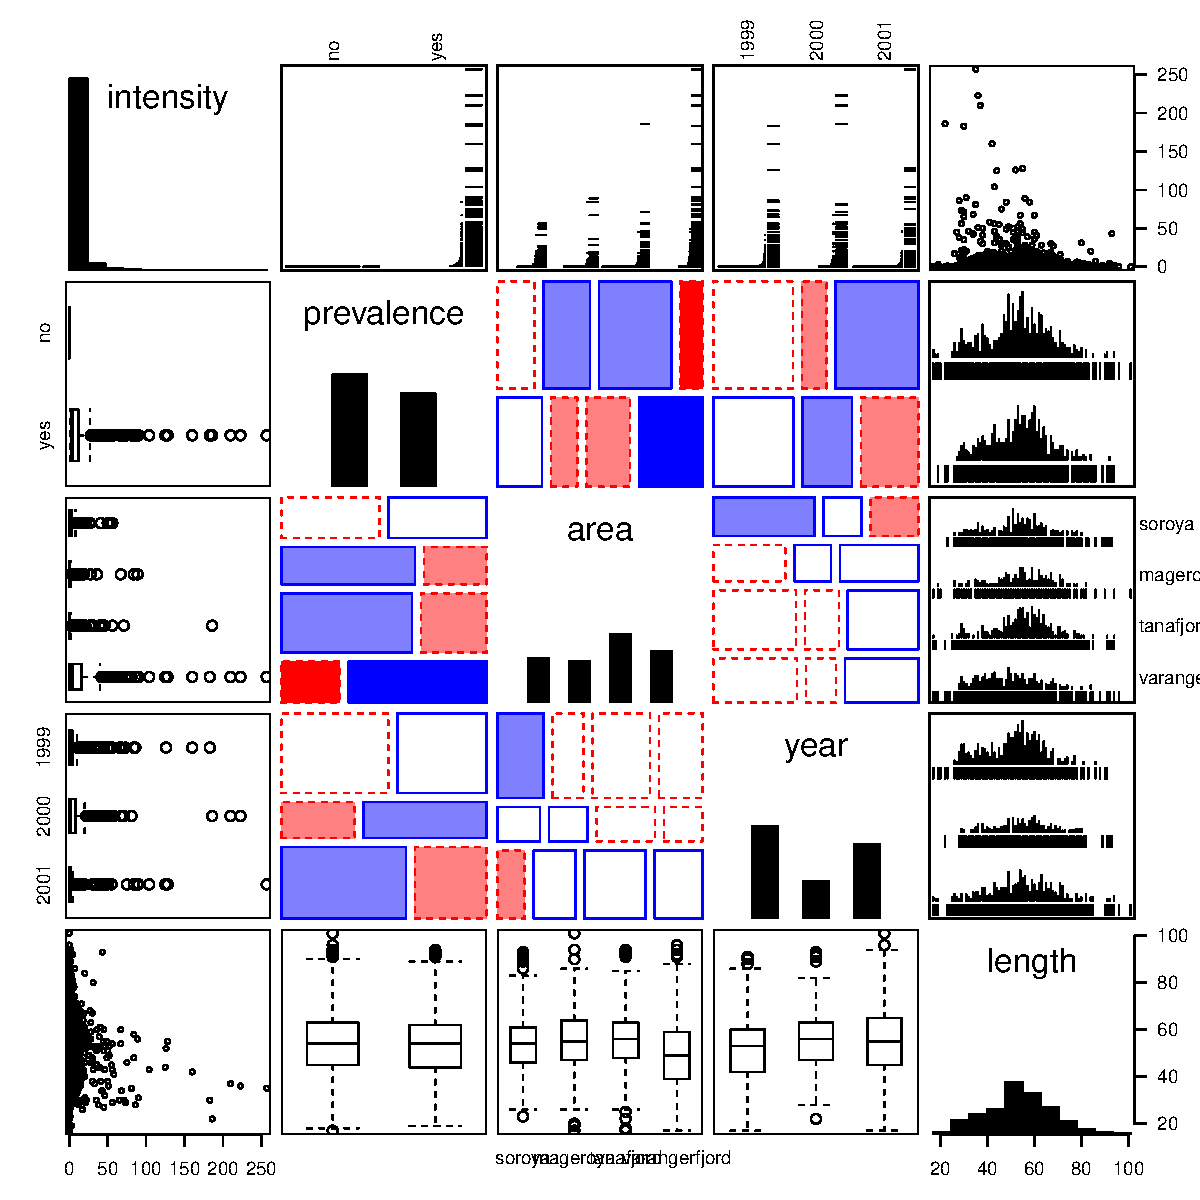
\includegraphics[width=.8\textwidth]{ch09/fig/cod1-gpairs-1} }

\caption[Generalized pairs plot for the CodParasites data]{Generalized pairs plot for the CodParasites data.\label{fig:cod1-gpairs}}
\end{figure}


\end{knitrout}
In this plot, among the categorical variables, prevalence is strongly associated with area, but also with year.
As well there seems to be an association between area and year, meaning the number of cod samples
collected in difference areas varied over time. In the univariate plots on the diagonal, intensity
stands out as extremely skewed, and the distribution of length appears reasonably symmetric.

Before fitting any models, some more detailed
exploratory plots are helpful for understanding the relationship
of both prevalence and intensity to the predictors.  The general idea is to make separate
plots of prevalence and intensity and to try to show both the data and some simple summaries.
In their Table 1, \citet{Hemmingsen-etal:2005}
counted the missing observations as infected and we do the same to get a similar contingency table.

\begin{knitrout}
\definecolor{shadecolor}{rgb}{1, 0.961, 0.933}\color{fgcolor}\begin{kframe}
\begin{alltt}
\hlstd{cp.tab} \hlkwb{<-} \hlkwd{xtabs}\hlstd{(}\hlopt{~} \hlstd{area} \hlopt{+} \hlstd{year} \hlopt{+} \hlkwd{factor}\hlstd{(}\hlkwd{is.na}\hlstd{(prevalence)} \hlopt{|}
                                       \hlstd{prevalence} \hlopt{==} \hlstr{"yes"}\hlstd{),}
                \hlkwc{data} \hlstd{= CodParasites)}
\hlkwd{dimnames}\hlstd{(cp.tab)[}\hlnum{3}\hlstd{]} \hlkwb{<-} \hlkwd{list}\hlstd{(}\hlkwd{c}\hlstd{(}\hlstr{"No"}\hlstd{,} \hlstr{"Yes"}\hlstd{))}
\hlkwd{names}\hlstd{(}\hlkwd{dimnames}\hlstd{(cp.tab))[}\hlnum{3}\hlstd{]} \hlkwb{<-} \hlstr{"prevalence"}
\end{alltt}
\end{kframe}
\end{knitrout}
For the factors \var{area} and \var{year}, we can visualize prevalence as before (\exref{ex:crabs-zero})
using spineplots, but, for two (or more) factors, doubledecker and mosaic plots are better because they
are more flexible and keep the factors distinct.  The doubledecker plot (\figref{fig:cod1-doubledecker})
highlights the infected fish, and shows that prevalence is indeed highest in all years in Varangerfjord.

\begin{knitrout}
\definecolor{shadecolor}{rgb}{1, 0.961, 0.933}\color{fgcolor}\begin{kframe}
\begin{alltt}
\hlkwd{doubledecker}\hlstd{(prevalence} \hlopt{~} \hlstd{area} \hlopt{+} \hlstd{year,} \hlkwc{data}\hlstd{=cp.tab)}
\end{alltt}
\end{kframe}\begin{figure}[!htbp]


\centerline{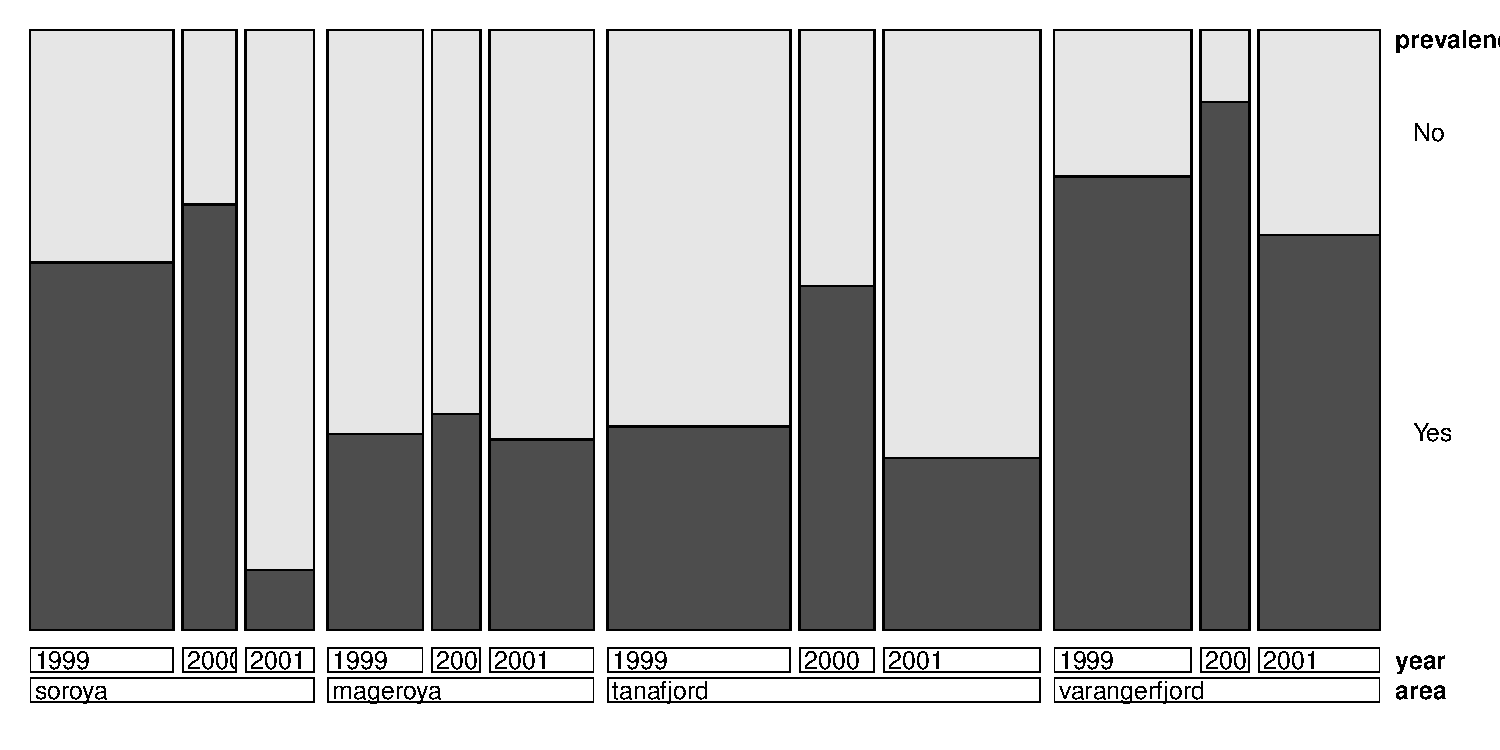
\includegraphics[width=.9\textwidth]{ch09/fig/cod1-doubledecker-1} }

\caption[Doubledecker plot for prevalence against area and year in the CodParasites data]{Doubledecker plot for prevalence against area and year in the CodParasites data. The cases of infected fish are hightlighted\label{fig:cod1-doubledecker}}
\end{figure}


\end{knitrout}
A similar plot, in the doubledecker format, can be drawn as a mosaic plot, but now shading the tiles
according a model for the expected counts.  It makes sense here to consider the null \loglin model
for prevalence as a response, independent of the combinations of area and year. This plot (\figref{fig:cod1-mosaic})
shows further that prevalence differs substantially over the area-year combinations, so we should expect
an interaction in the model for zero counts. As well, Varangerfjord stands out as having consistently
greater prevalence in all years than expected under this model.

\begin{knitrout}
\definecolor{shadecolor}{rgb}{1, 0.961, 0.933}\color{fgcolor}\begin{kframe}
\begin{alltt}
\hlkwd{mosaic}\hlstd{(}\hlopt{~}\hlstd{area} \hlopt{+} \hlstd{year} \hlopt{+} \hlstd{prevalence,} \hlkwc{data}\hlstd{=cp.tab,}
       \hlkwc{split_vertical}\hlstd{=}\hlkwd{c}\hlstd{(}\hlnum{TRUE}\hlstd{,} \hlnum{TRUE}\hlstd{,} \hlnum{FALSE}\hlstd{),}
       \hlkwc{labeling}\hlstd{=labeling_doubledecker,} \hlkwc{spacing}\hlstd{=spacing_highlighting,}
       \hlkwc{expected} \hlstd{=} \hlopt{~}\hlstd{year}\hlopt{:}\hlstd{area} \hlopt{+} \hlstd{prevalence)}
\end{alltt}
\end{kframe}\begin{figure}[!htbp]


\centerline{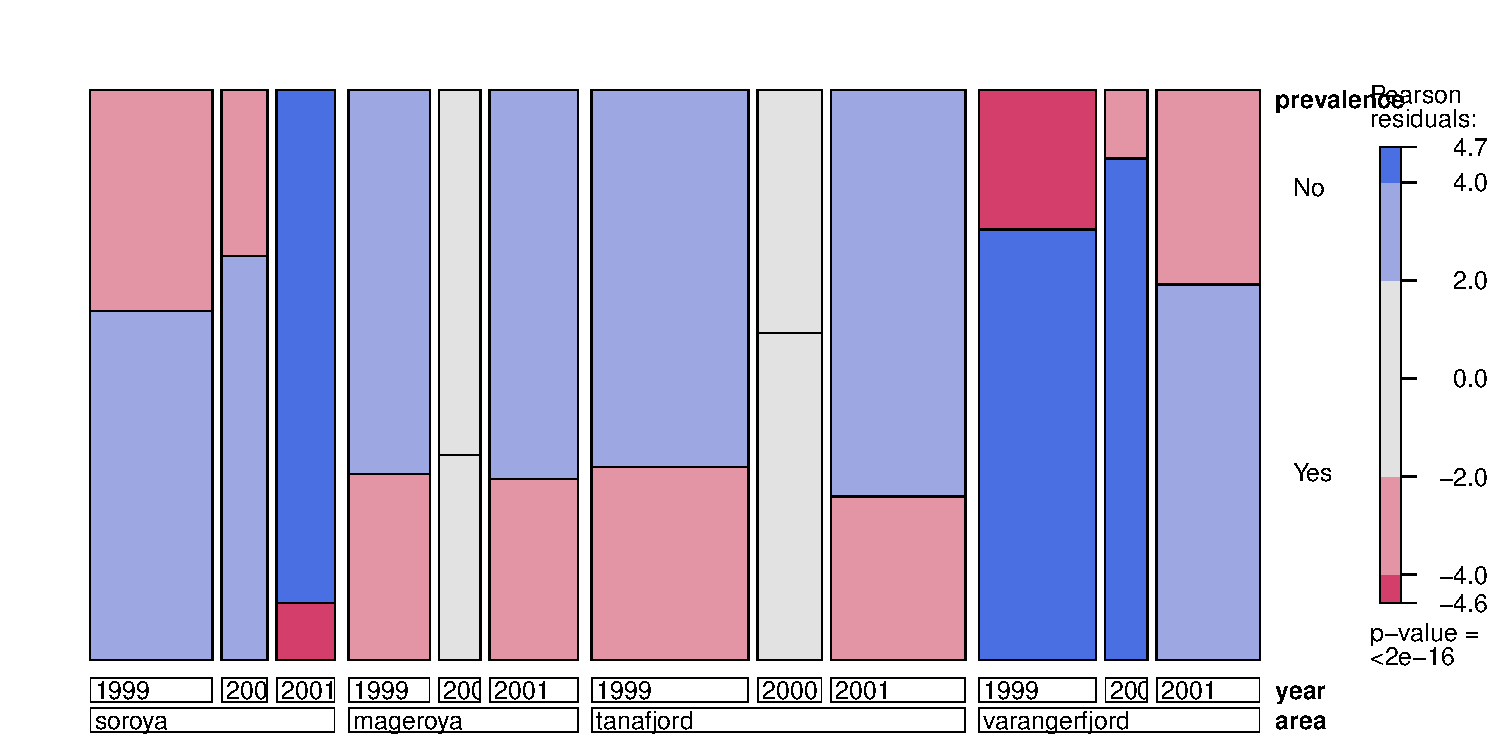
\includegraphics[width=.9\textwidth]{ch09/fig/cod1-mosaic-1} }

\caption[Mosaic plot for prevalence against area and year in the CodParasites data, in the doubledecker format]{Mosaic plot for prevalence against area and year in the CodParasites data, in the doubledecker format. Shading reflects departure from a model in which prevalence is independent of area and year jointly.\label{fig:cod1-mosaic}}
\end{figure}


\end{knitrout}
The effect of fish \var{length} on \var{prevalence} can be most easily seen by treating the factor as
a numeric (0/1) variable and smoothing, as shown in \figref{fig:cod1-length-prevalence}.
The loess smoothed curve shows an apparent U-shaped relationship, however the plotted observations
and the confidence bands make clear that there is very little data in the extremes of \var{length}.

\begin{knitrout}
\definecolor{shadecolor}{rgb}{1, 0.961, 0.933}\color{fgcolor}\begin{kframe}
\begin{alltt}
\hlkwd{library}\hlstd{(ggplot2)}
\hlkwd{ggplot}\hlstd{(CodParasites,} \hlkwd{aes}\hlstd{(}\hlkwc{x}\hlstd{=length,} \hlkwc{y}\hlstd{=}\hlkwd{as.numeric}\hlstd{(prevalence)}\hlopt{-}\hlnum{1}\hlstd{))} \hlopt{+}
  \hlkwd{geom_jitter}\hlstd{(}\hlkwc{position}\hlstd{=}\hlkwd{position_jitter}\hlstd{(}\hlkwc{height}\hlstd{=}\hlnum{.05}\hlstd{),} \hlkwc{alpha}\hlstd{=}\hlnum{0.25}\hlstd{)} \hlopt{+}
  \hlkwd{geom_rug}\hlstd{(}\hlkwc{position}\hlstd{=}\hlstr{'jitter'}\hlstd{,} \hlkwc{sides}\hlstd{=}\hlstr{'b'}\hlstd{)} \hlopt{+}
  \hlkwd{stat_smooth}\hlstd{(}\hlkwc{method}\hlstd{=}\hlstr{"loess"}\hlstd{,} \hlkwc{color}\hlstd{=}\hlstr{"red"}\hlstd{,} \hlkwc{fill}\hlstd{=}\hlstr{"red"}\hlstd{,} \hlkwc{size}\hlstd{=}\hlnum{1.5}\hlstd{)} \hlopt{+}
  \hlkwd{theme_bw}\hlstd{()} \hlopt{+} \hlkwd{labs}\hlstd{(}\hlkwc{y}\hlstd{=}\hlstr{'prevalence'}\hlstd{)}
\end{alltt}
\end{kframe}\begin{figure}[!htbp]


\centerline{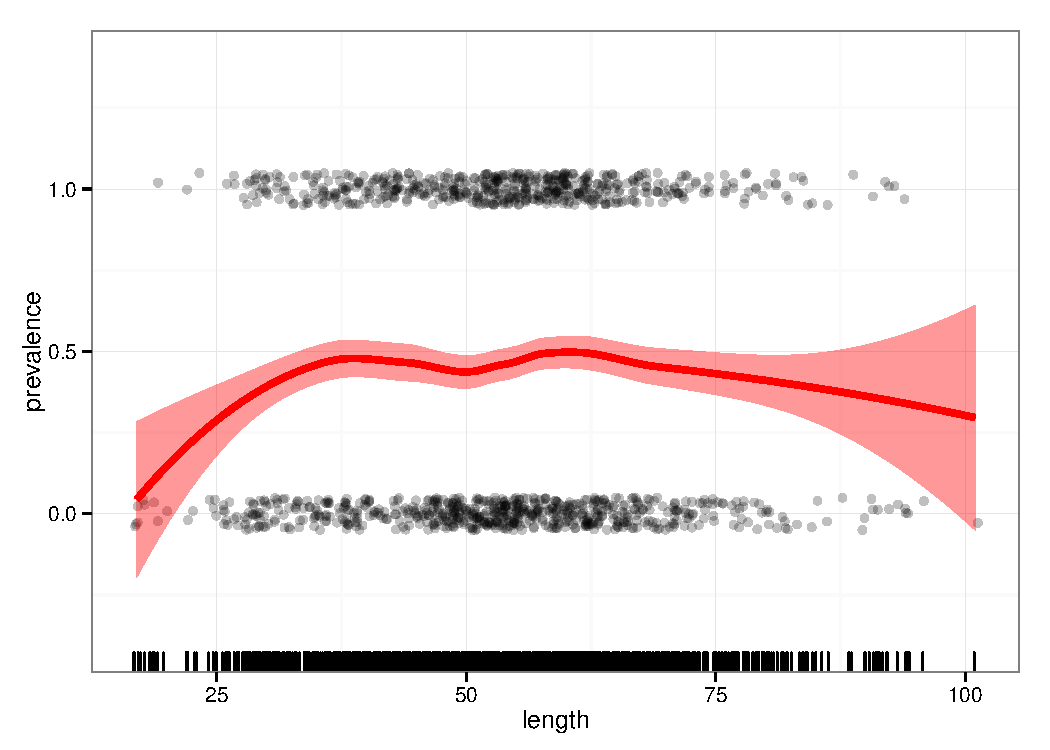
\includegraphics[width=.6\textwidth]{ch09/fig/cod1-length-prevalence-1} }

\caption[Jittered scatterplot of prevalence against length of fish, with loess smooth]{Jittered scatterplot of prevalence against length of fish, with loess smooth.\label{fig:cod1-length-prevalence}}
\end{figure}


\end{knitrout}


For the positive counts of \var{intensity}, boxplots by area and year show the distributions of parasites,
and it is again useful to display these on a log scale.
In \figref{fig:cod1-boxplot}, we have used \pkg{ggplot2},
with \func{geom\_boxplot} and \func{geom\_jitter} to also plot the individual observations.
Note that \func{facet\_grid} makes it easy to organize the display with separate panels for each
area, a technique that could extend to additional factors.

\begin{knitrout}
\definecolor{shadecolor}{rgb}{1, 0.961, 0.933}\color{fgcolor}\begin{kframe}
\begin{alltt}
\hlcom{# plot only positive values of intensity}
\hlstd{CPpos} \hlkwb{<-} \hlkwd{subset}\hlstd{(CodParasites, intensity}\hlopt{>}\hlnum{0}\hlstd{)}
\hlkwd{ggplot}\hlstd{(CPpos,} \hlkwd{aes}\hlstd{(}\hlkwc{x}\hlstd{=year,} \hlkwc{y}\hlstd{=intensity))} \hlopt{+}
  \hlkwd{geom_boxplot}\hlstd{(}\hlkwc{outlier.size}\hlstd{=}\hlnum{3}\hlstd{,} \hlkwc{notch}\hlstd{=}\hlnum{TRUE}\hlstd{,} \hlkwd{aes}\hlstd{(}\hlkwc{fill}\hlstd{=year),} \hlkwc{alpha}\hlstd{=}\hlnum{0.2}\hlstd{)} \hlopt{+}
  \hlkwd{geom_jitter}\hlstd{(}\hlkwc{position}\hlstd{=}\hlkwd{position_jitter}\hlstd{(}\hlkwc{width}\hlstd{=}\hlnum{0.1}\hlstd{),} \hlkwc{alpha}\hlstd{=}\hlnum{0.25}\hlstd{)} \hlopt{+}
  \hlkwd{facet_grid}\hlstd{(.}\hlopt{~}\hlstd{area)} \hlopt{+}
  \hlkwd{scale_y_log10}\hlstd{(}\hlkwc{breaks}\hlstd{=}\hlkwd{c}\hlstd{(}\hlnum{1}\hlstd{,}\hlnum{2}\hlstd{,}\hlnum{5}\hlstd{,}\hlnum{10}\hlstd{,}\hlnum{20}\hlstd{,}\hlnum{50}\hlstd{,}\hlnum{100}\hlstd{,} \hlnum{200}\hlstd{))} \hlopt{+}
  \hlkwd{theme_bw}\hlstd{()} \hlopt{+} \hlkwd{theme}\hlstd{(}\hlkwc{legend.position}\hlstd{=}\hlstr{"none"}\hlstd{)} \hlopt{+}
  \hlkwd{labs}\hlstd{(}\hlkwc{y}\hlstd{=}\hlstr{'intensity (log scale)'}\hlstd{)}
\end{alltt}
\end{kframe}\begin{figure}[!htbp]


\centerline{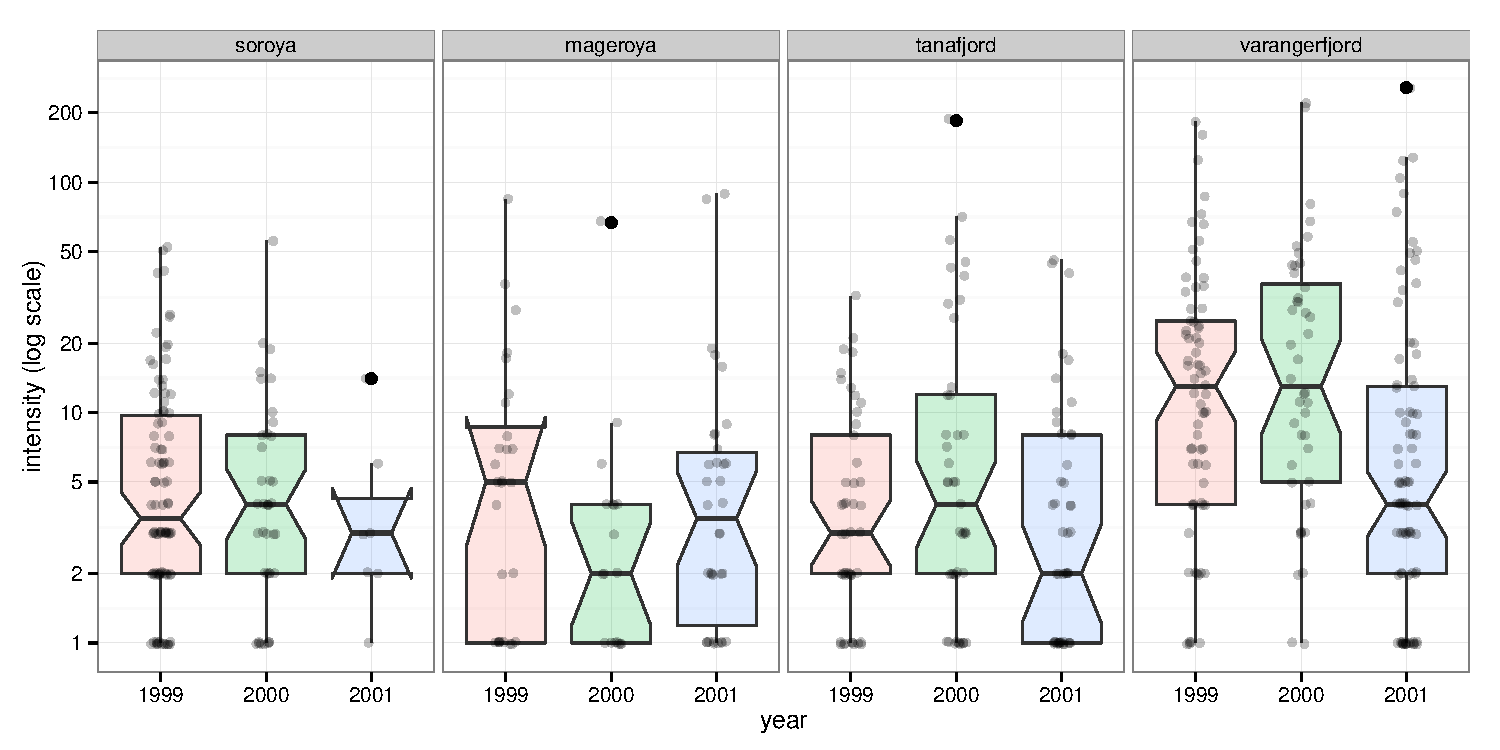
\includegraphics[width=.9\textwidth]{ch09/fig/cod1-boxplot-1} }

\caption[Notched boxplots for log (intensity) of parasites by area and year in the CodParasites data]{Notched boxplots for log (intensity) of parasites by area and year in the CodParasites data. Significant differences in the medians are signaled when the notches of two groups do not overlap.\label{fig:cod1-boxplot}}
\end{figure}


\end{knitrout}
Most of these distributions are positively skewed and
there are a few high outliers, but probably not more than would be expected in a sample of this size.
The positive counts (degree of infection) are also higher in all years in Varangerfjord than other
areas. You can also see that the intensity values were generally lower in 2001 than other years.

For the effect of length of fish, we want to know if log (intensity) is reasonably
linear on length.  A jittered scatterplot produced with \pkg{ggplot2} is shown in \figref{fig:cod1-length-scat}.
The smoothed loess curve together with the linear regression line show no indication of non-linearity.

\begin{knitrout}
\definecolor{shadecolor}{rgb}{1, 0.961, 0.933}\color{fgcolor}\begin{kframe}
\begin{alltt}
\hlkwd{ggplot}\hlstd{(CPpos,} \hlkwd{aes}\hlstd{(}\hlkwc{x}\hlstd{=length,} \hlkwc{y}\hlstd{=intensity))} \hlopt{+}
  \hlkwd{geom_jitter}\hlstd{(}\hlkwc{position}\hlstd{=}\hlkwd{position_jitter}\hlstd{(}\hlkwc{height}\hlstd{=}\hlnum{.1}\hlstd{),} \hlkwc{alpha}\hlstd{=}\hlnum{0.25}\hlstd{)} \hlopt{+}
  \hlkwd{geom_rug}\hlstd{(}\hlkwc{position}\hlstd{=}\hlstr{'jitter'}\hlstd{,} \hlkwc{sides}\hlstd{=}\hlstr{'b'}\hlstd{)} \hlopt{+}
  \hlkwd{scale_y_log10}\hlstd{(}\hlkwc{breaks}\hlstd{=}\hlkwd{c}\hlstd{(}\hlnum{1}\hlstd{,}\hlnum{2}\hlstd{,}\hlnum{5}\hlstd{,}\hlnum{10}\hlstd{,}\hlnum{20}\hlstd{,}\hlnum{50}\hlstd{,}\hlnum{100}\hlstd{,} \hlnum{200}\hlstd{))} \hlopt{+}
  \hlkwd{stat_smooth}\hlstd{(}\hlkwc{method}\hlstd{=}\hlstr{"loess"}\hlstd{,} \hlkwc{color}\hlstd{=}\hlstr{"red"}\hlstd{,} \hlkwc{fill}\hlstd{=}\hlstr{"red"}\hlstd{,} \hlkwc{size}\hlstd{=}\hlnum{2}\hlstd{)} \hlopt{+}
  \hlkwd{stat_smooth}\hlstd{(}\hlkwc{method}\hlstd{=}\hlstr{"lm"}\hlstd{,} \hlkwc{size}\hlstd{=}\hlnum{1.5}\hlstd{)} \hlopt{+} \hlkwd{theme_bw}\hlstd{()}
\end{alltt}
\end{kframe}\begin{figure}[!htbp]


\centerline{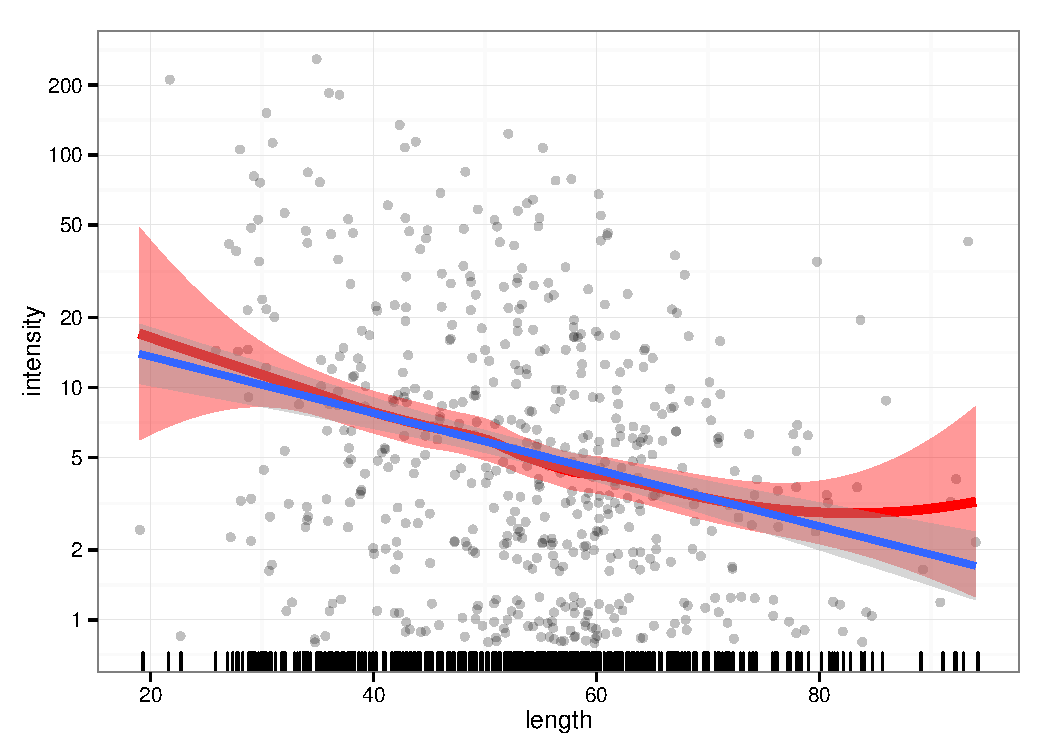
\includegraphics[width=.6\textwidth]{ch09/fig/cod1-length-scat-1} }

\caption[Jittered scatterplot of log (intensity) for the positive counts against length of fish, with loess smooth and linear regression line]{Jittered scatterplot of log (intensity) for the positive counts against length of fish, with loess smooth and linear regression line.\label{fig:cod1-length-scat}}
\end{figure}


\end{knitrout}
\end{Example}

\subsubsection{Fitting models}

The simple summary of these exploratory analyses is that both the zero component (prevalence) and
and non-zero component (intensity)
involve an interaction of \var{area} and \var{year} and at least intensity depends on \var{length}.
We proceed to fit some count data models.

\begin{Example}[cod2]{Cod parasites}
For a baseline reference, we first fit the standard Poisson and negative-binomial models, not
allowing for excess zeros.
\begin{knitrout}
\definecolor{shadecolor}{rgb}{1, 0.961, 0.933}\color{fgcolor}\begin{kframe}
\begin{alltt}
\hlkwd{library}\hlstd{(MASS);} \hlkwd{library}\hlstd{(countreg)}
\hlstd{cp_p}   \hlkwb{<-}    \hlkwd{glm}\hlstd{(intensity} \hlopt{~} \hlstd{length} \hlopt{+} \hlstd{area} \hlopt{*} \hlstd{year,}
                 \hlkwc{data} \hlstd{= CodParasites,} \hlkwc{family} \hlstd{= poisson)}
\hlstd{cp_nb}  \hlkwb{<-} \hlkwd{glm.nb}\hlstd{(intensity} \hlopt{~} \hlstd{length} \hlopt{+} \hlstd{area} \hlopt{*} \hlstd{year,}
                 \hlkwc{data} \hlstd{= CodParasites)}
\end{alltt}
\end{kframe}
\end{knitrout}

Next, we fit analogous hurdle and zero-inflated models, in each case allowing the non-zero
count component to be either Poisson or negative-binomial. The zero components are fit
as logistic regressions with the same predictors and the logit link.
\begin{knitrout}
\definecolor{shadecolor}{rgb}{1, 0.961, 0.933}\color{fgcolor}\begin{kframe}
\begin{alltt}
\hlstd{cp_hp}  \hlkwb{<-} \hlkwd{hurdle}\hlstd{(intensity} \hlopt{~} \hlstd{length} \hlopt{+} \hlstd{area} \hlopt{*} \hlstd{year,}
                 \hlkwc{data} \hlstd{= CodParasites,} \hlkwc{dist} \hlstd{=} \hlstr{"poisson"}\hlstd{)}
\hlstd{cp_hnb} \hlkwb{<-} \hlkwd{hurdle}\hlstd{(intensity} \hlopt{~} \hlstd{length} \hlopt{+} \hlstd{area} \hlopt{*} \hlstd{year,}
                 \hlkwc{data} \hlstd{= CodParasites,} \hlkwc{dist} \hlstd{=} \hlstr{"negbin"}\hlstd{)}
\hlstd{cp_zip} \hlkwb{<-} \hlkwd{zeroinfl}\hlstd{(intensity} \hlopt{~} \hlstd{length} \hlopt{+} \hlstd{area} \hlopt{*} \hlstd{year,}
                   \hlkwc{data} \hlstd{= CodParasites,} \hlkwc{dist} \hlstd{=} \hlstr{"poisson"}\hlstd{)}
\hlstd{cp_znb} \hlkwb{<-} \hlkwd{zeroinfl}\hlstd{(intensity} \hlopt{~} \hlstd{length} \hlopt{+} \hlstd{area} \hlopt{*} \hlstd{year,}
                   \hlkwc{data} \hlstd{= CodParasites,} \hlkwc{dist} \hlstd{=} \hlstr{"negbin"}\hlstd{)}
\end{alltt}
\end{kframe}
\end{knitrout}
Following \secref{sec:glm-visfit}, we can compare the fit of these models using rootograms.
The details of fit of these six models are shown in \figref{fig:cod2-rootograms}.
\begin{knitrout}
\definecolor{shadecolor}{rgb}{1, 0.961, 0.933}\color{fgcolor}\begin{kframe}
\begin{alltt}
\hlstd{op} \hlkwb{<-} \hlkwd{par}\hlstd{(}\hlkwc{mfrow} \hlstd{=} \hlkwd{c}\hlstd{(}\hlnum{3}\hlstd{,} \hlnum{2}\hlstd{))}
\hlstd{countreg::}\hlkwd{rootogram}\hlstd{(cp_p,} \hlkwc{max} \hlstd{=} \hlnum{50}\hlstd{,} \hlkwc{main} \hlstd{=} \hlstr{"Poisson"}\hlstd{)}
\hlstd{countreg::}\hlkwd{rootogram}\hlstd{(cp_nb,} \hlkwc{max} \hlstd{=} \hlnum{50}\hlstd{,} \hlkwc{main} \hlstd{=} \hlstr{"Negative Binomial"}\hlstd{)}
\hlstd{countreg::}\hlkwd{rootogram}\hlstd{(cp_hp,} \hlkwc{max} \hlstd{=} \hlnum{50}\hlstd{,} \hlkwc{main} \hlstd{=} \hlstr{"Hurdle Poisson"}\hlstd{)}
\hlstd{countreg::}\hlkwd{rootogram}\hlstd{(cp_hnb,} \hlkwc{max} \hlstd{=} \hlnum{50}\hlstd{,} \hlkwc{main} \hlstd{=} \hlstr{"Hurdle Negative Binomial"}\hlstd{)}
\hlstd{countreg::}\hlkwd{rootogram}\hlstd{(cp_zip,} \hlkwc{max} \hlstd{=} \hlnum{50}\hlstd{,} \hlkwc{main} \hlstd{=} \hlstr{"Zero-inflated Poisson"}\hlstd{)}
\hlstd{countreg::}\hlkwd{rootogram}\hlstd{(cp_znb,} \hlkwc{max} \hlstd{=} \hlnum{50}\hlstd{,} \hlkwc{main} \hlstd{=} \hlstr{"Zero-inflated Negative Binomial"}\hlstd{)}
\hlkwd{par}\hlstd{(op)}
\end{alltt}
\end{kframe}\begin{figure}[!htbp]


\centerline{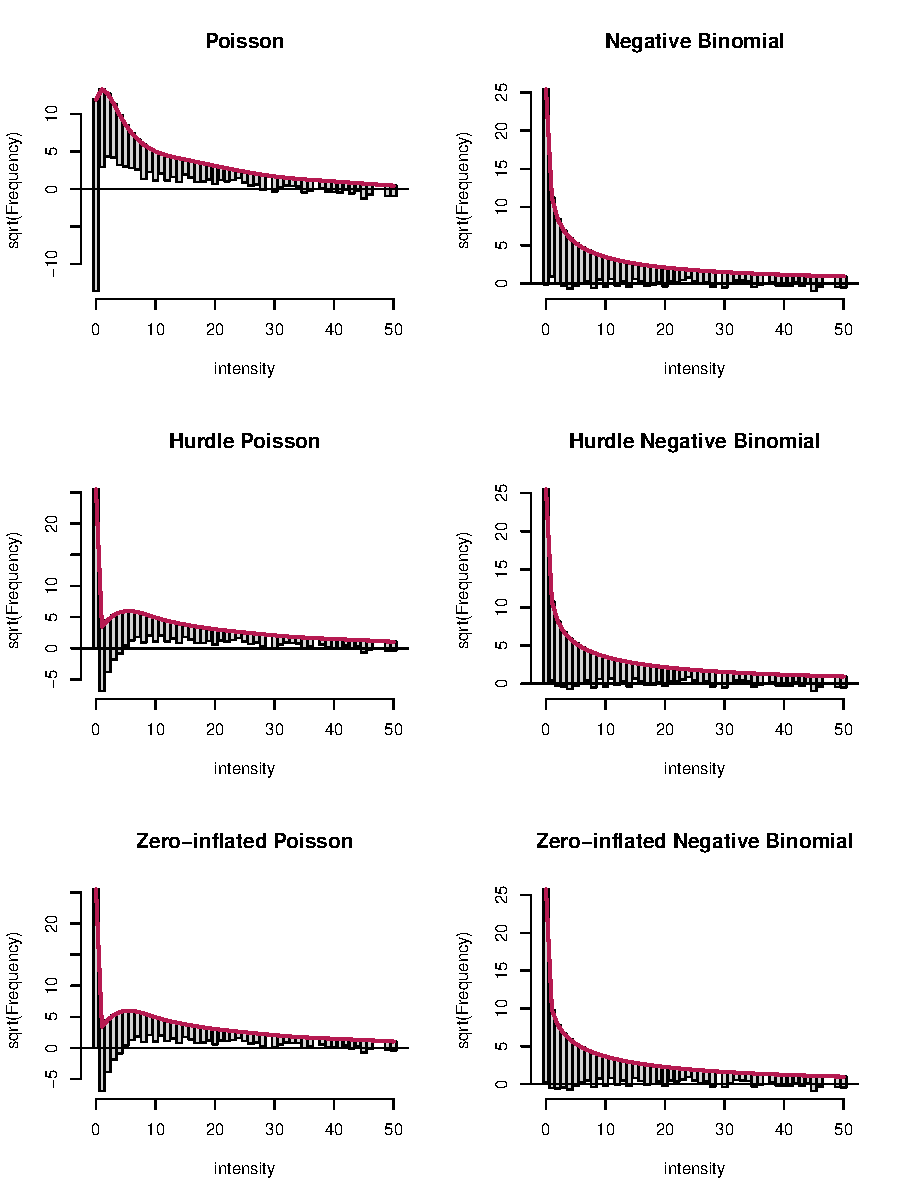
\includegraphics[width=.8\textwidth]{ch09/fig/cod2-rootograms-1} }

\caption[Rootograms for six models fit to the CodParasites data]{Rootograms for six models fit to the CodParasites data\label{fig:cod2-rootograms}}
\end{figure}


\end{knitrout}
The basic Poisson model of course fits terribly due to the excess zero counts.
The hurdle Poisson and zero-inflated Poisson fit the zero counts perfectly, but
at the expense of underfitting the counts for low intensity values.
All of the negative binomial models show a reasonable fit (at the scale shown in this plot),
and none show a systematic pattern of under/overfitting.

These models are all in different GLM and extended-GLM families, and there are no
\func{anova} methods for hurdle and zero-inflated models.
Each pair of
Poisson and negative-binomial models are a nested set, because the
Poisson is a special case of the negative-binomial where $\theta \rightarrow \infty$,
and so can be compared using \LR tests available with \func{lrtest} from \pkg{lmtest}.
However, this cannot be used to compare models of different class,
such as a hurdle model vs.\ a zero-inflated model.
(In \figref{fig:cod2-rootograms}, each pair in the same row are nested models,
while all other pairs are non-nested.)
Yet, they all have \func{logLik}
methods to calculate their log likelihood, and so \func{AIC} and \func{BIC}
can be used.
%\TODO{Update vcdExtra for this.}

\begin{knitrout}
\definecolor{shadecolor}{rgb}{1, 0.961, 0.933}\color{fgcolor}\begin{kframe}
\begin{alltt}
\hlstd{vcdExtra::}\hlkwd{Summarise}\hlstd{(cp_p, cp_nb, cp_hp, cp_hnb, cp_zip, cp_znb,} \hlkwc{sortby}\hlstd{=}\hlstr{"BIC"}\hlstd{)}
\end{alltt}
\begin{verbatim}
## Likelihood summary table:
##          AIC   BIC LR Chisq   Df Pr(>Chisq)    
## cp_p   20378 20444    20352 1178     <2e-16 ***
## cp_hp  13688 13820    13636 1165     <2e-16 ***
## cp_zip 13687 13819    13635 1165     <2e-16 ***
## cp_nb   5031  5102     5003 1178     <2e-16 ***
## cp_znb  4955  5092     4901 1164     <2e-16 ***
## cp_hnb  4937  5074     4883 1164     <2e-16 ***
## ---
## Signif. codes:  0 '***' 0.001 '**' 0.01 '*' 0.05 '.' 0.1 ' ' 1
\end{verbatim}
\end{kframe}
\end{knitrout}

These show that all the Poisson models fit quite badly, and among the negative-binomial models,
the hurdle version, \code{cp\_hnb}, is preferred by both AIC and BIC.
If you want to carry out formal tests, \func{lrtest} can be used to compare
a given Poisson model to its negative-binomial counterpart, which are nested.
For example, the test below compares the hurdle Poisson to the hurdle
negative-binomial and confirms that the latter is a significant improvement.
\begin{knitrout}
\definecolor{shadecolor}{rgb}{1, 0.961, 0.933}\color{fgcolor}\begin{kframe}
\begin{alltt}
\hlkwd{library}\hlstd{(lmtest)}
\hlkwd{lrtest}\hlstd{(cp_hp, cp_hnb)}
\end{alltt}
\begin{verbatim}
## Likelihood ratio test
## 
## Model 1: intensity ~ length + area * year
## Model 2: intensity ~ length + area * year
##   #Df LogLik Df Chisq Pr(>Chisq)    
## 1  26  -6818                        
## 2  27  -2442  1  8752     <2e-16 ***
## ---
## Signif. codes:  0 '***' 0.001 '**' 0.01 '*' 0.05 '.' 0.1 ' ' 1
\end{verbatim}
\end{kframe}
\end{knitrout}
Of greater interest is the difference among the negative-binomial models,
that are not nested.  As described in \secref{sec:glm-nonnest},
these can be compared using Voung's test.
\begin{knitrout}
\definecolor{shadecolor}{rgb}{1, 0.961, 0.933}\color{fgcolor}\begin{kframe}
\begin{alltt}
\hlkwd{library}\hlstd{(pscl)}
\hlkwd{vuong}\hlstd{(cp_nb, cp_hnb)}     \hlcom{# nb vs. hurdle nb}
\end{alltt}
\begin{verbatim}
## Vuong Non-Nested Hypothesis Test-Statistic: 40.549 
## (test-statistic is asymptotically distributed N(0,1) under the
##  null that the models are indistinguishible)
## in this case:
## model1 > model2, with p-value <2e-16
\end{verbatim}
\begin{alltt}
\hlkwd{vuong}\hlstd{(cp_hnb, cp_znb)}    \hlcom{# hurdle nb vs znb}
\end{alltt}
\begin{verbatim}
## Vuong Non-Nested Hypothesis Test-Statistic: 1.7941 
## (test-statistic is asymptotically distributed N(0,1) under the
##  null that the models are indistinguishible)
## in this case:
## model1 > model2, with p-value 0.0364
\end{verbatim}
\end{kframe}
\end{knitrout}
The negative-binomial model is considered to be a closer fit
than the hurdle version (because it is more parsimonious),
while the hurdle NB model has a significantly better fit than the zero-inflated
NB model.  For this example, we continue to work with the hurdle NB model.
The tests for individual coefficients in this model are shown below.
\begin{knitrout}\footnotesize
\definecolor{shadecolor}{rgb}{1, 0.961, 0.933}\color{fgcolor}\begin{kframe}
\begin{alltt}
\hlkwd{summary}\hlstd{(cp_hnb)}
\end{alltt}
\begin{verbatim}
...
## Count model coefficients (truncated negbin with log link):
##                            Estimate Std. Error z value Pr(>|z|)    
## (Intercept)                 3.37580    0.39947    8.45  < 2e-16 ***
## length                     -0.03748    0.00587   -6.38  1.7e-10 ***
## areamageroya                0.37898    0.38105    0.99   0.3199    
## areatanafjord              -0.50480    0.31238   -1.62   0.1061    
## areavarangerfjord           0.89159    0.29161    3.06   0.0022 ** 
## year2000                   -0.03957    0.32857   -0.12   0.9041    
## year2001                   -0.75388    0.68925   -1.09   0.2741    
## areamageroya:year2000      -0.63981    0.61667   -1.04   0.2995    
## areatanafjord:year2000      1.19387    0.49479    2.41   0.0158 *  
## areavarangerfjord:year2000  0.51074    0.47719    1.07   0.2845    
## areamageroya:year2001       0.70444    0.82036    0.86   0.3905    
## areatanafjord:year2001      0.90824    0.77685    1.17   0.2424    
## areavarangerfjord:year2001  0.59838    0.74738    0.80   0.4233    
## Log(theta)                 -1.49866    0.23904   -6.27  3.6e-10 ***
## Zero hurdle model coefficients (binomial with logit link):
##                            Estimate Std. Error z value Pr(>|z|)    
## (Intercept)                 0.08526    0.29505    0.29    0.773    
## length                      0.00693    0.00465    1.49    0.136    
## areamageroya               -1.32137    0.28526   -4.63  3.6e-06 ***
## areatanafjord              -1.44918    0.24388   -5.94  2.8e-09 ***
## areavarangerfjord           0.30073    0.27111    1.11    0.267    
## year2000                    0.39507    0.34382    1.15    0.251    
## year2001                   -2.65201    0.43340   -6.12  9.4e-10 ***
## areamageroya:year2000      -0.08034    0.50797   -0.16    0.874    
## areatanafjord:year2000      0.87058    0.45027    1.93    0.053 .  
## areavarangerfjord:year2000  0.86462    0.59239    1.46    0.144    
## areamageroya:year2001       2.73749    0.53291    5.14  2.8e-07 ***
## areatanafjord:year2001      2.71899    0.49949    5.44  5.2e-08 ***
## areavarangerfjord:year2001  2.54144    0.51825    4.90  9.4e-07 ***
## ---
## Signif. codes:  0 '***' 0.001 '**' 0.01 '*' 0.05 '.' 0.1 ' ' 1 
## 
## Theta: count = 0.223
## Number of iterations in BFGS optimization: 25 
## Log-likelihood: -2.44e+03 on 27 Df
...
\end{verbatim}
\end{kframe}
\end{knitrout}
From the above and from \figref{fig:cod1-length-prevalence}, it appears that
\var{length} is not important as a linear effect in the submodel for
prevalence.  A revised model excludes this from the zero formula.

\begin{knitrout}
\definecolor{shadecolor}{rgb}{1, 0.961, 0.933}\color{fgcolor}\begin{kframe}
\begin{alltt}
\hlstd{cp_hnb1} \hlkwb{<-} \hlkwd{hurdle}\hlstd{(intensity} \hlopt{~} \hlstd{length} \hlopt{+} \hlstd{area} \hlopt{*} \hlstd{year} \hlopt{|} \hlstd{area}\hlopt{*}\hlstd{year,}
                  \hlkwc{data} \hlstd{= CodParasites,} \hlkwc{dist} \hlstd{=} \hlstr{"negbin"}\hlstd{)}
\end{alltt}
\end{kframe}
\end{knitrout}

A \LR test shows no advantage for the smaller model, however
Vuong's test leads to the conclusion that this reduced model is preferable:
\begin{knitrout}
\definecolor{shadecolor}{rgb}{1, 0.961, 0.933}\color{fgcolor}\begin{kframe}
\begin{alltt}
\hlkwd{lrtest}\hlstd{(cp_hnb, cp_hnb1)}
\end{alltt}
\begin{verbatim}
## Likelihood ratio test
## 
## Model 1: intensity ~ length + area * year
## Model 2: intensity ~ length + area * year | area * year
##   #Df LogLik Df Chisq Pr(>Chisq)
## 1  27  -2442                    
## 2  26  -2443 -1  2.23       0.14
\end{verbatim}
\begin{alltt}
\hlkwd{vuong}\hlstd{(cp_hnb, cp_hnb1)}
\end{alltt}
\begin{verbatim}
## Vuong Non-Nested Hypothesis Test-Statistic: -2.7995 
## (test-statistic is asymptotically distributed N(0,1) under the
##  null that the models are indistinguishible)
## in this case:
## model2 > model1, with p-value 0.00256
\end{verbatim}
\end{kframe}
\end{knitrout}


\end{Example}

\subsubsection{Model interpretation: Effect plots}

Interpreting these models from their coefficients is very difficult because an interaction
is present and there are separate submodels for the zero and count components.
This task is much easier with effects plots.
The \Rpackage{effects} has methods for any GLM, but cannot handle the extended forms of
the zero-inflated and hurdle models.

When the same predictors are used in both
submodels, and a standard GLM such as the negative-binomial provides a reasonable
fit, you can use the standard \pkg{effects} functions to visualize the (total)
expected count, which for the zeros would include both the extra zeros and
those that derive from the count submodel.  For visual interpretation, these will
be sufficiently similar, even though the hurdle and zero-inflated models differ
with respect to explaining overdispersion and/or excess zeros.

Alternatively, if you want to visualize and interpret the zero and nonzero components
separately, perhaps with different predictors, you can fit the implied submodels
separately, and then use \pkg{effects} functions for the effects in each.
These ideas are illustrated in the next example.

\begin{Example}[cod3]{Cod parasites}
The expected counts for \var{intensity}, including both zero and positive counts
can be plotted using \pkg{effects} for the \code{cp_nb} NB model.
\figref{fig:cod2-rootograms} gives some confidence that the fitted values
are similar to those in the hurdle and zero-inflated versions.

We use \func{allEffects} to calculate the effects for the high-order terms--- the
main effect of \var{length} and the interaction of \var{area} and \var{year}.
These could be plotted together by plotting the resulting \code{eff.nb} object,
but we plot them separately to control the plot details.  In these plots,
the argument \code{rescale=FALSE} gives plots on the response scale, and
we use \code{ylim} to equate the ranges to make the plots directly comparable.
The code below produces \figref{fig:cod2-eff1}.

\begin{knitrout}
\definecolor{shadecolor}{rgb}{1, 0.961, 0.933}\color{fgcolor}\begin{kframe}
\begin{alltt}
\hlkwd{library}\hlstd{(effects)}
\hlstd{eff.nb} \hlkwb{<-} \hlkwd{allEffects}\hlstd{(cp_nb)}
\hlkwd{plot}\hlstd{(eff.nb[}\hlnum{1}\hlstd{],} \hlkwc{rescale}\hlstd{=}\hlnum{FALSE}\hlstd{,} \hlkwc{ylim}\hlstd{=}\hlkwd{c}\hlstd{(}\hlnum{0}\hlstd{,}\hlnum{30}\hlstd{),}
     \hlkwc{main}\hlstd{=}\hlstr{"NB model: length effect"}\hlstd{)}

\hlkwd{plot}\hlstd{(eff.nb[}\hlnum{2}\hlstd{],} \hlkwc{rescale}\hlstd{=}\hlnum{FALSE}\hlstd{,} \hlkwc{ylim}\hlstd{=}\hlkwd{c}\hlstd{(}\hlnum{0}\hlstd{,}\hlnum{30}\hlstd{),}
     \hlkwc{multiline}\hlstd{=}\hlnum{TRUE}\hlstd{,} \hlkwc{ci.style}\hlstd{=}\hlstr{'bars'}\hlstd{,}
     \hlkwc{key.args}\hlstd{=}\hlkwd{list}\hlstd{(}\hlkwc{x}\hlstd{=}\hlnum{.05}\hlstd{,} \hlkwc{y}\hlstd{=}\hlnum{.95}\hlstd{),}
     \hlkwc{colors}\hlstd{=}\hlkwd{c}\hlstd{(}\hlstr{"black"}\hlstd{,} \hlstr{"red"}\hlstd{,} \hlstr{"blue"}\hlstd{) ,}
     \hlkwc{symbols}\hlstd{=}\hlnum{15}\hlopt{:}\hlnum{17}\hlstd{,} \hlkwc{cex}\hlstd{=}\hlnum{2}\hlstd{,}
     \hlkwc{main}\hlstd{=}\hlstr{"NB model: area*year effect"}\hlstd{)}
\end{alltt}
\end{kframe}\begin{figure}[!htbp]


\centerline{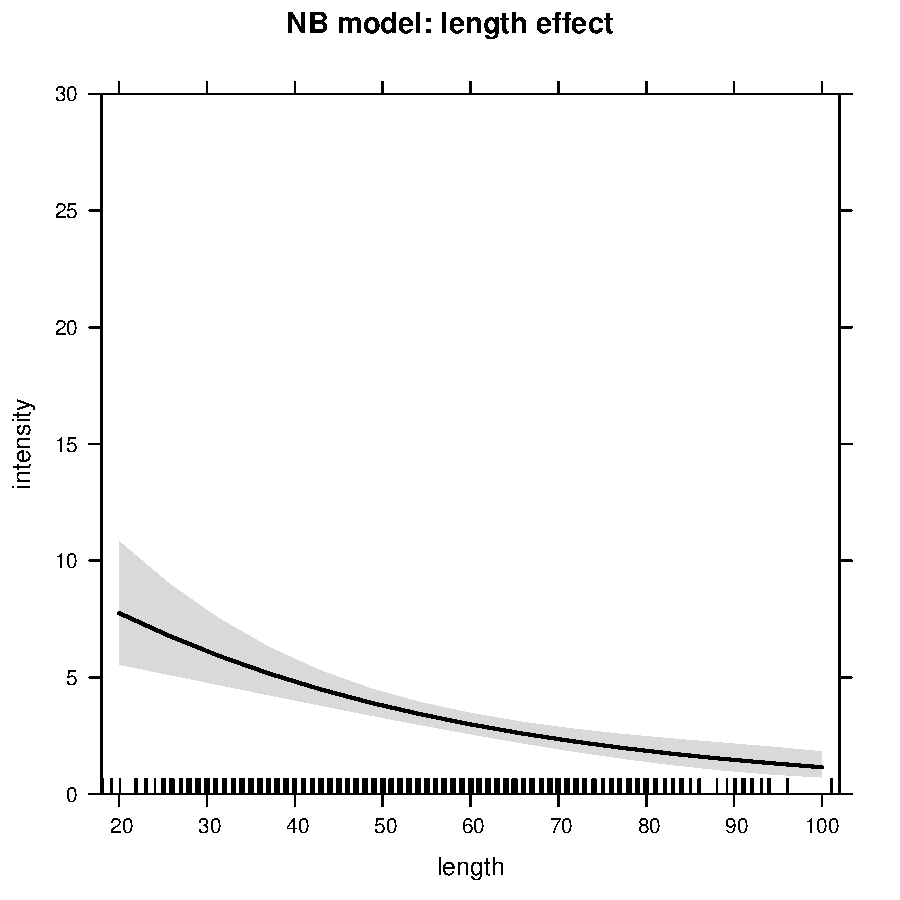
\includegraphics[width=.49\textwidth]{ch09/fig/cod3-eff1-1} 
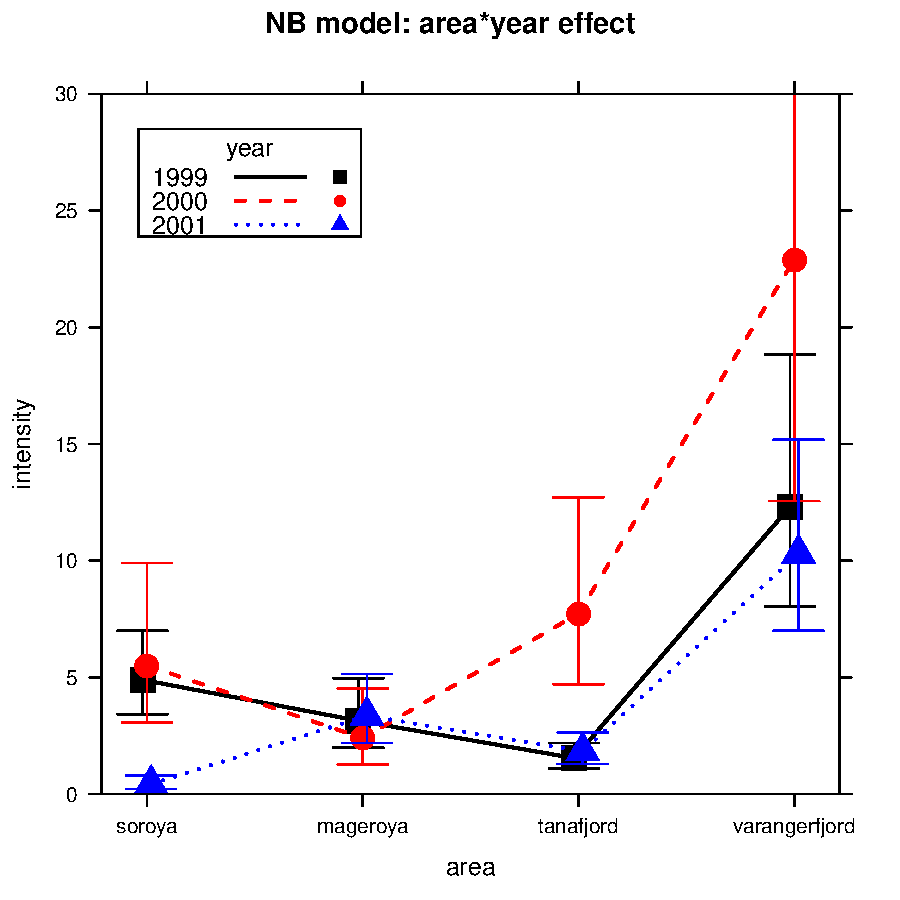
\includegraphics[width=.49\textwidth]{ch09/fig/cod3-eff1-2} }

\caption[Effect plots for total intensity of parasites from the negative-binomial model]{Effect plots for total intensity of parasites from the negative-binomial model\label{fig:cod3-eff1}}
\end{figure}


\end{knitrout}
This helps to interpret the nature of the area by year effect.  The pattern of mean expected
intensity of cod parasites is similar in 1999 and 2001, except for the S{\o}r{\o}ya area.
The results in year 2000 differ mainly in greater intensity in Tanafjord and Varangerfjord.
Varangerfjord shows larger infection counts overall, but particularly in year 2000.
The effect plot for length on this scale is roughly comparable to the variation in
areas and years.

In this example, the submodels for zero and positive counts have substantively different
interpretations. To visualize the fitted effects in these submodels using \pkg{effects},
first fit the equivalent submodels separately using GLM methods. The following
models for \var{prevalence}, using the binomial family,
and the positive counts for \var{intensity}, using \func{glm.nb},
give similar fitted
results to those obtained from the hurdle negative-binomial model, \code{cp\_hnb}
discussed earlier.

\begin{knitrout}
\definecolor{shadecolor}{rgb}{1, 0.961, 0.933}\color{fgcolor}\begin{kframe}
\begin{alltt}
\hlstd{cp_zero}  \hlkwb{<-} \hlkwd{glm}\hlstd{(prevalence} \hlopt{~} \hlstd{length} \hlopt{+} \hlstd{area} \hlopt{*} \hlstd{year,}
                \hlkwc{data} \hlstd{= CodParasites,} \hlkwc{family}\hlstd{=binomial)}
\hlstd{cp_nzero} \hlkwb{<-} \hlkwd{glm.nb}\hlstd{(intensity} \hlopt{~} \hlstd{length} \hlopt{+} \hlstd{area} \hlopt{*} \hlstd{year,}
                   \hlkwc{data} \hlstd{= CodParasites,} \hlkwc{subset}\hlstd{=intensity}\hlopt{>}\hlnum{0}\hlstd{)}
\end{alltt}
\end{kframe}
\end{knitrout}
We could construct effect plots for each of these submodels, but interest here is largely on the
binomial model for the zero counts, \code{cp\_zero}. Effect plots for the terms in this model
are shown in \figref{fig:cod3-eff2}.  Again, we set the \code{ylim} values to equate the
vertical ranges to make the plots comparable.
\begin{knitrout}
\definecolor{shadecolor}{rgb}{1, 0.961, 0.933}\color{fgcolor}\begin{kframe}
\begin{alltt}
\hlstd{eff.zero} \hlkwb{<-} \hlkwd{allEffects}\hlstd{(cp_zero)}
\hlkwd{plot}\hlstd{(eff.zero[}\hlnum{1}\hlstd{],} \hlkwc{ylim}\hlstd{=}\hlkwd{c}\hlstd{(}\hlopt{-}\hlnum{2.5}\hlstd{,} \hlnum{2.5}\hlstd{),}
     \hlkwc{main}\hlstd{=}\hlstr{"Hurdle zero model: length effect"}\hlstd{)}

\hlkwd{plot}\hlstd{(eff.zero[}\hlnum{2}\hlstd{],}  \hlkwc{ylim}\hlstd{=}\hlkwd{c}\hlstd{(}\hlopt{-}\hlnum{2.5}\hlstd{,} \hlnum{2.5}\hlstd{),}
     \hlkwc{multiline}\hlstd{=}\hlnum{TRUE}\hlstd{,}
     \hlkwc{key.args}\hlstd{=}\hlkwd{list}\hlstd{(}\hlkwc{x}\hlstd{=}\hlnum{.05}\hlstd{,} \hlkwc{y}\hlstd{=}\hlnum{.95}\hlstd{),}
     \hlkwc{colors}\hlstd{=}\hlkwd{c}\hlstd{(}\hlstr{"black"}\hlstd{,} \hlstr{"red"}\hlstd{,} \hlstr{"blue"}\hlstd{),}
     \hlkwc{symbols}\hlstd{=}\hlnum{15}\hlopt{:}\hlnum{17}\hlstd{,} \hlkwc{cex}\hlstd{=}\hlnum{2}\hlstd{,}
     \hlkwc{main}\hlstd{=}\hlstr{"Hurdle zero model: area*year effect"}\hlstd{)}
\end{alltt}
\end{kframe}\begin{figure}[!htbp]


\centerline{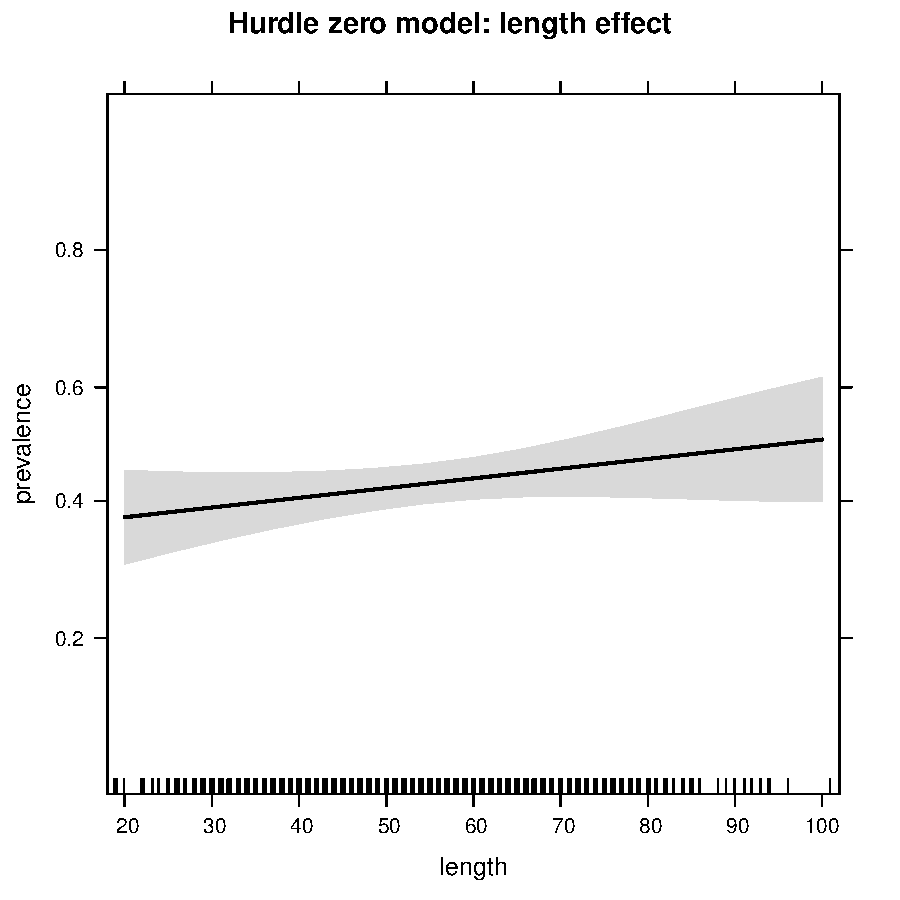
\includegraphics[width=.49\textwidth]{ch09/fig/cod3-eff2-1} 
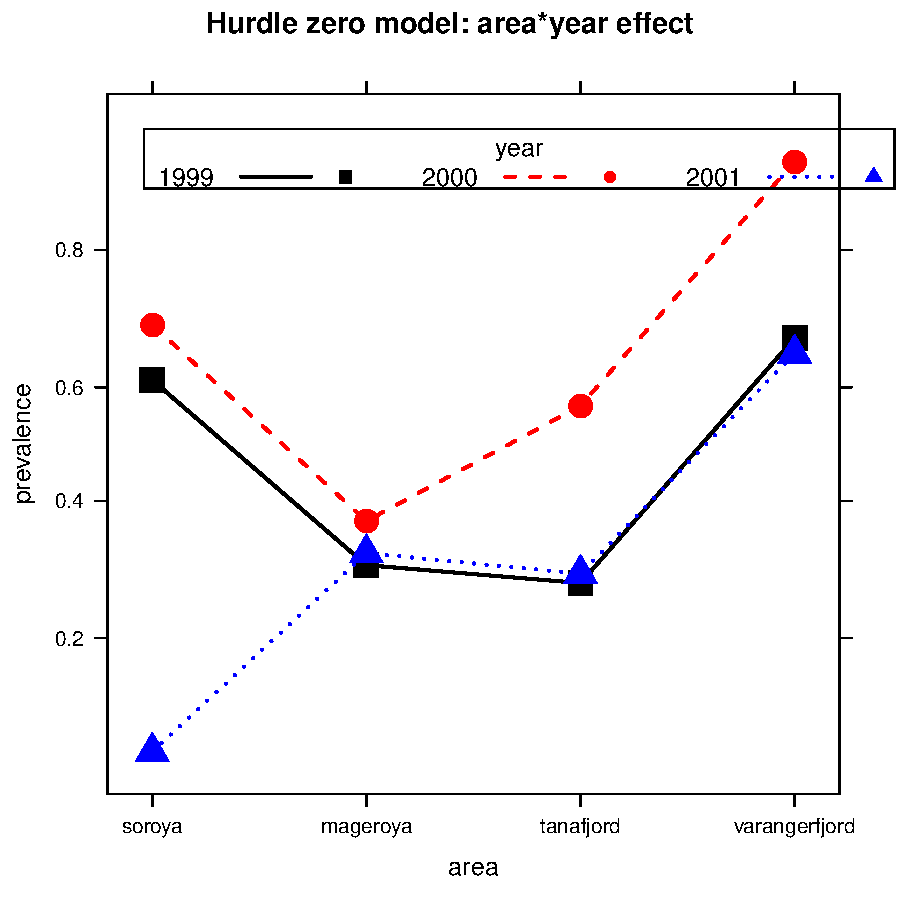
\includegraphics[width=.49\textwidth]{ch09/fig/cod3-eff2-2} }

\caption[Effect plots for prevalence of parasites analogous to  the hurdle negative-binomial model, fitted using a binomial GLM model]{Effect plots for prevalence of parasites analogous to  the hurdle negative-binomial model, fitted using a binomial GLM model.\label{fig:cod3-eff2}}
\end{figure}


\end{knitrout}
The effect of \var{length} on prevalence is slightly increasing, but we saw earlier that this is
not significant.  For the area-year interaction, the three curves have similar shapes, except
for the aberrant value for S{\o}r{\o}ya in 2001 and the closeness of the values at
Mager{\o}ya in all years. Overall, prevalence was highest in 2000, and also in
the Varangerfjord samples.

\end{Example}


\subsection{Demand for medical care by the elderly}\label{sec:glm-case-nmes}

A large cross-sectional study was carried out by the U.S. National Medical Expenditure
Survey (NMES) in 1987--1988 to assess the demand for medical care, as
measured by the number of physician/non-physician office visits and the
number of hospital outpatient visits to a physician/non-physician.
The survey was based upon a representative, national probability sample of the civilian non-institutionalized population and individuals admitted to long-term care facilities during 1987.  A subsample of 4,406
individuals ages 66 and over, all of whom are covered by Medicare is contained
in the \data{NMES1988} data set in the \Rpackage{AER}.
These data were previously analyzed by \citet{DebTrivedi:1997}
and \citet{Zeileis-etal:2008}, from which this account borrows.
The objective of the study and these analyses is to create a descriptive, and hopefully predictive, model
for the demand for medical care in this elderly population.


\begin{Example}[nmes1]{Demand for medical care}

The potential response variables in the \data{NMES1988} data set
form a $2 \times 2$ set of the combinations
of \emph{place of visit} (office vs.\ hospital) and (physician vs.\ non-physician) \emph{practitioner}.
Here, we focus on the highest total frequency
variable \var{visits}, recording office visits to a physician.
There are quite a few potential predictors, but here we consider only
the following:
\begin{itemize*}
\item \var{hospital}: number of hospital stays%
\footnote{
It is arguable that number of hospitalizations should be regarded as a
dependent variable, reflecting another aspect of demand for medical care,
rather than as a predictor.  We include it here as a predictor to control
for its relationship to the outcome \var{visits}.
}
\item \var{health}: a factor indicating self-perceived health status, with categories
  \code{"poor"}, \code{"average"} (reference category), \code{"excellent"}
\item \var{chronic}:  number of chronic conditions
\item \var{gender}
\item \var{school}:  number of years of education
\item \var{insurance}: a factor. Is the individual covered by private insurance?
\end{itemize*}
For convenience, these variables are extracted to a reduced data set, \code{nmes}.
\begin{knitrout}
\definecolor{shadecolor}{rgb}{1, 0.961, 0.933}\color{fgcolor}\begin{kframe}
\begin{alltt}
\hlkwd{data}\hlstd{(}\hlstr{"NMES1988"}\hlstd{,} \hlkwc{package}\hlstd{=}\hlstr{"AER"}\hlstd{)}
\hlstd{nmes} \hlkwb{<-} \hlstd{NMES1988[,} \hlkwd{c}\hlstd{(}\hlnum{1}\hlstd{,} \hlnum{6}\hlopt{:}\hlnum{8}\hlstd{,} \hlnum{13}\hlstd{,} \hlnum{15}\hlstd{,} \hlnum{18}\hlstd{)]}
\end{alltt}
\end{kframe}
\end{knitrout}
A quick overview of the response variable, \var{visits} is shown as simple (unbinned) histograms
on the frequency and log(frequency) scales in \figref{fig:nmes-visits}.
The zero counts are not as extreme as we have seen in other examples. On the log scale, there
is a small, but noticeable spike at 0, followed by a progressive, nearly linear decline, up to about
30 visits.
\begin{knitrout}
\definecolor{shadecolor}{rgb}{1, 0.961, 0.933}\color{fgcolor}\begin{kframe}
\begin{alltt}
\hlkwd{plot}\hlstd{(}\hlkwd{table}\hlstd{(nmes}\hlopt{$}\hlstd{visits),}
     \hlkwc{xlab}\hlstd{=}\hlstr{"Physician office visits"}\hlstd{,} \hlkwc{ylab}\hlstd{=}\hlstr{"Frequency"}\hlstd{)}
\hlkwd{plot}\hlstd{(}\hlkwd{log}\hlstd{(}\hlkwd{table}\hlstd{(nmes}\hlopt{$}\hlstd{visits)),}
     \hlkwc{xlab}\hlstd{=}\hlstr{"Physician office visits"}\hlstd{,} \hlkwc{ylab}\hlstd{=}\hlstr{"log(Frequency)"}\hlstd{)}
\end{alltt}
\end{kframe}\begin{figure}[!htbp]


\centerline{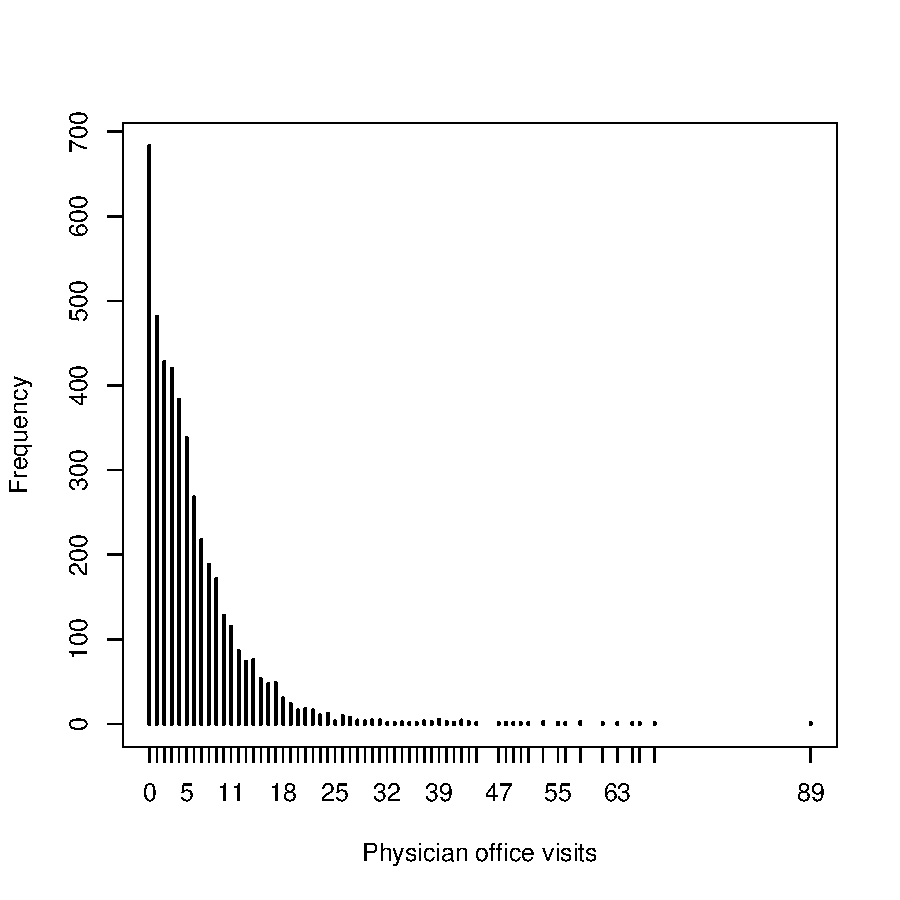
\includegraphics[width=.49\textwidth]{ch09/fig/nmes-visits-1} 
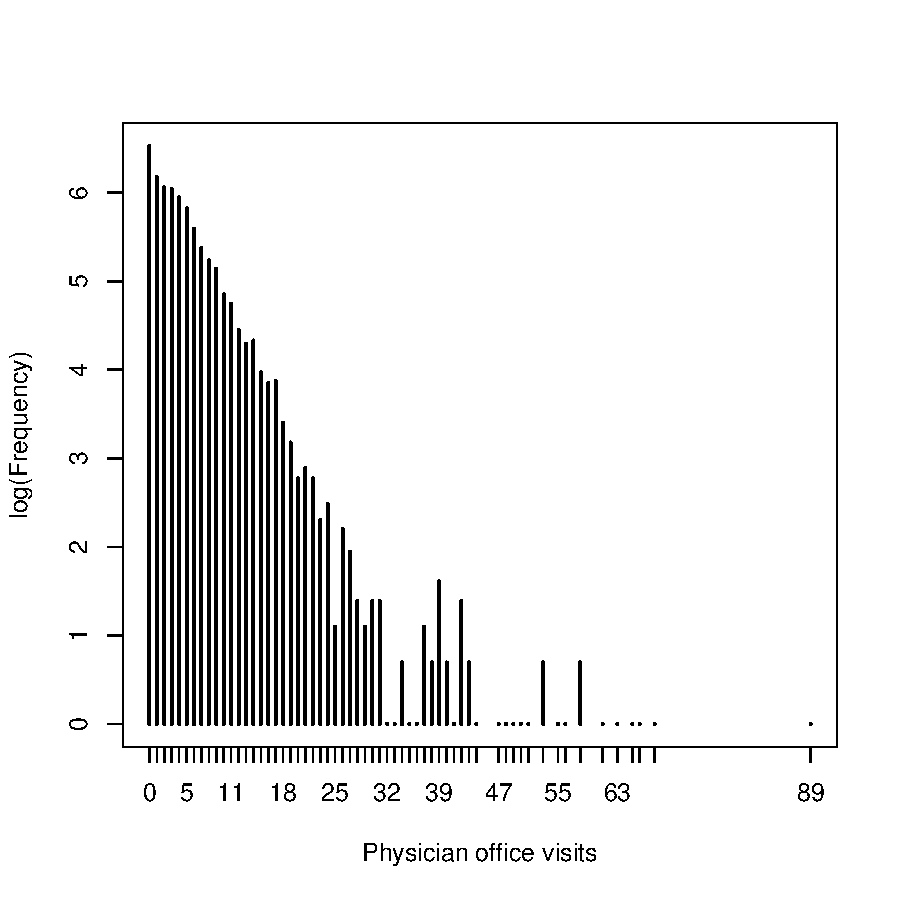
\includegraphics[width=.49\textwidth]{ch09/fig/nmes-visits-2} }

\caption[Frequency distributions of the number of physician office visits]{Frequency distributions of the number of physician office visits\label{fig:nmes-visits}}
\end{figure}


\end{knitrout}
However as a benchmark, without taking any predictors into account, there is very substantial
overdispersion relative to a Poisson distribution, the variance being nearly 8 times the mean.
\begin{knitrout}
\definecolor{shadecolor}{rgb}{1, 0.961, 0.933}\color{fgcolor}\begin{kframe}
\begin{alltt}
\hlkwd{with}\hlstd{(nmes,}  \hlkwd{c}\hlstd{(}\hlkwc{mean}\hlstd{=}\hlkwd{mean}\hlstd{(visits),}
              \hlkwc{var}\hlstd{=}\hlkwd{var}\hlstd{(visits),}
              \hlkwc{ratio}\hlstd{=}\hlkwd{var}\hlstd{(visits)}\hlopt{/}\hlkwd{mean}\hlstd{(visits)))}
\end{alltt}
\begin{verbatim}
##    mean     var   ratio 
##  5.7744 45.6871  7.9120
\end{verbatim}
\end{kframe}
\end{knitrout}
As before, it is useful to precede formal analysis with a variety of exploratory plots.
\figref{fig:nmes-boxplots} shows a few of these as boxplots, using \func{cutfac} to make
predictors discrete, and plotting \var{visits} on a log scale, started at 1.
All of these show the expected relationships, e.g., number of office
visits increases with numbers of chronic conditions and hospital stays,
but decreases with better perceived health status.
\begin{knitrout}
\definecolor{shadecolor}{rgb}{1, 0.961, 0.933}\color{fgcolor}\begin{kframe}
\begin{alltt}
\hlstd{op} \hlkwb{<-}\hlkwd{par}\hlstd{(}\hlkwc{mfrow}\hlstd{=}\hlkwd{c}\hlstd{(}\hlnum{1}\hlstd{,} \hlnum{3}\hlstd{),} \hlkwc{cex.lab}\hlstd{=}\hlnum{1.4}\hlstd{)}
\hlkwd{plot}\hlstd{(}\hlkwd{log}\hlstd{(visits}\hlopt{+}\hlnum{1}\hlstd{)} \hlopt{~} \hlkwd{cutfac}\hlstd{(chronic),} \hlkwc{data} \hlstd{= nmes,}
     \hlkwc{ylab} \hlstd{=} \hlstr{"Physician office visits (log scale)"}\hlstd{,}
     \hlkwc{xlab} \hlstd{=} \hlstr{"Number of chronic conditions"}\hlstd{,} \hlkwc{main} \hlstd{=} \hlstr{"chronic"}\hlstd{)}
\hlkwd{plot}\hlstd{(}\hlkwd{log}\hlstd{(visits}\hlopt{+}\hlnum{1}\hlstd{)} \hlopt{~} \hlstd{health,} \hlkwc{data} \hlstd{= nmes,} \hlkwc{varwidth} \hlstd{=} \hlnum{TRUE}\hlstd{,}
     \hlkwc{ylab} \hlstd{=} \hlstr{"Physician office visits (log scale)"}\hlstd{,}
     \hlkwc{xlab} \hlstd{=} \hlstr{"Self-perceived health status"}\hlstd{,} \hlkwc{main} \hlstd{=} \hlstr{"health"}\hlstd{)}
\hlkwd{plot}\hlstd{(}\hlkwd{log}\hlstd{(visits}\hlopt{+}\hlnum{1}\hlstd{)} \hlopt{~} \hlkwd{cutfac}\hlstd{(hospital,} \hlkwd{c}\hlstd{(}\hlnum{0}\hlopt{:}\hlnum{2}\hlstd{,} \hlnum{8}\hlstd{)),} \hlkwc{data} \hlstd{= nmes,}
     \hlkwc{ylab} \hlstd{=} \hlstr{"Physician office visits (log scale)"}\hlstd{,}
     \hlkwc{xlab} \hlstd{=} \hlstr{"Number of hospital stays"}\hlstd{,} \hlkwc{main} \hlstd{=} \hlstr{"hospital"}\hlstd{)}
\hlkwd{par}\hlstd{(op)}
\end{alltt}
\end{kframe}\begin{figure}[!htbp]


\centerline{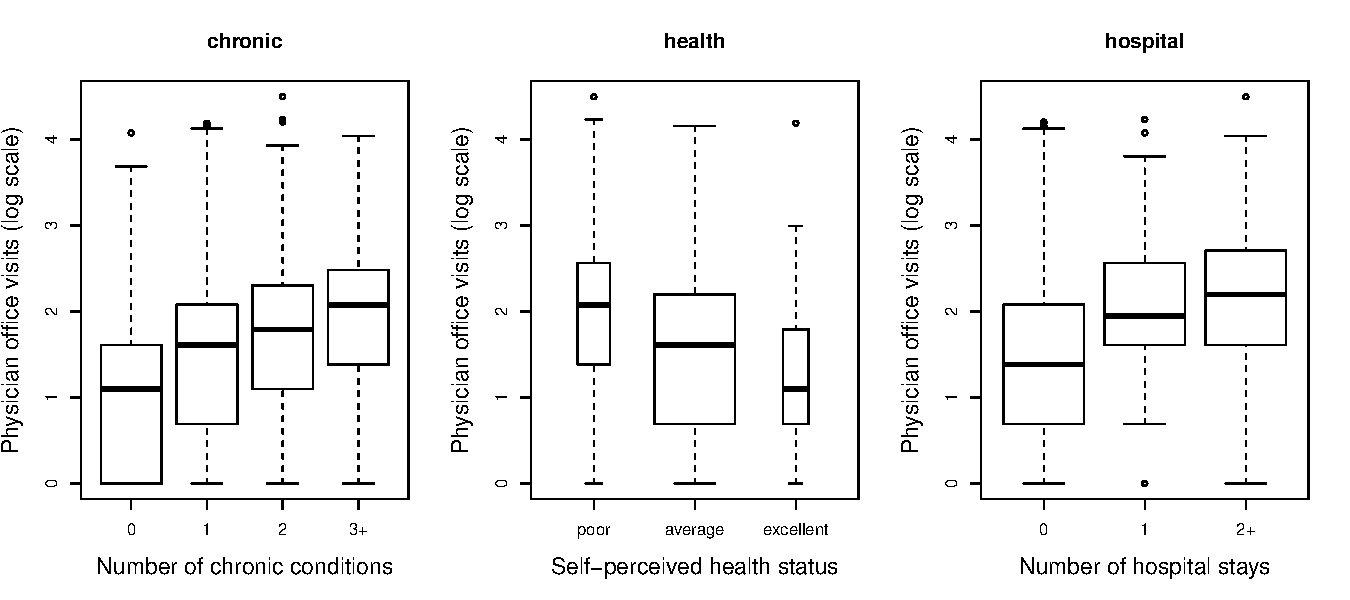
\includegraphics[width=\textwidth]{ch09/fig/nmes-boxplots-1} }

\caption[Number of physician office visits plotted against some of the predictors]{Number of physician office visits plotted against some of the predictors\label{fig:nmes-boxplots}}
\end{figure}


\end{knitrout}
\noindent Similar plots for \var{insurance} and \var{gender} show that those with private insurance
have more office visits and women slightly more than men.

The relationship with number of years of education could be shown in boxplots by the use of
\code{cutfac(school)}, or with \func{spineplot} by making both variables discrete.
However, it is more informative (shows the data)
to depict this in a smoothed and jittered scatterplot,
as in \figref{fig:nmes-school}.
\begin{knitrout}
\definecolor{shadecolor}{rgb}{1, 0.961, 0.933}\color{fgcolor}\begin{kframe}
\begin{alltt}
\hlkwd{library}\hlstd{(ggplot2)}
\hlkwd{ggplot}\hlstd{(nmes,} \hlkwd{aes}\hlstd{(}\hlkwc{x}\hlstd{=school,} \hlkwc{y}\hlstd{=visits}\hlopt{+}\hlnum{1}\hlstd{))} \hlopt{+}
  \hlkwd{geom_jitter}\hlstd{(}\hlkwc{alpha}\hlstd{=}\hlnum{0.25}\hlstd{)} \hlopt{+}
  \hlkwd{stat_smooth}\hlstd{(}\hlkwc{method}\hlstd{=}\hlstr{"loess"}\hlstd{,} \hlkwc{color}\hlstd{=}\hlstr{"red"}\hlstd{,} \hlkwc{fill}\hlstd{=}\hlstr{"red"}\hlstd{,} \hlkwc{size}\hlstd{=}\hlnum{1.5}\hlstd{,} \hlkwc{alpha}\hlstd{=}\hlnum{0.3}\hlstd{)} \hlopt{+}
  \hlkwd{labs}\hlstd{(}\hlkwc{x}\hlstd{=}\hlstr{"Number of years of education"}\hlstd{,} \hlkwc{y}\hlstd{=}\hlstr{"log(Physician office visits+1)"}\hlstd{)} \hlopt{+}
  \hlkwd{scale_y_log10}\hlstd{(}\hlkwc{breaks}\hlstd{=}\hlkwd{c}\hlstd{(}\hlnum{1}\hlstd{,}\hlnum{2}\hlstd{,}\hlnum{5}\hlstd{,}\hlnum{10}\hlstd{,}\hlnum{20}\hlstd{,}\hlnum{50}\hlstd{,}\hlnum{100}\hlstd{))} \hlopt{+} \hlkwd{theme_bw}\hlstd{()}
\end{alltt}
\end{kframe}\begin{figure}[!htbp]


\centerline{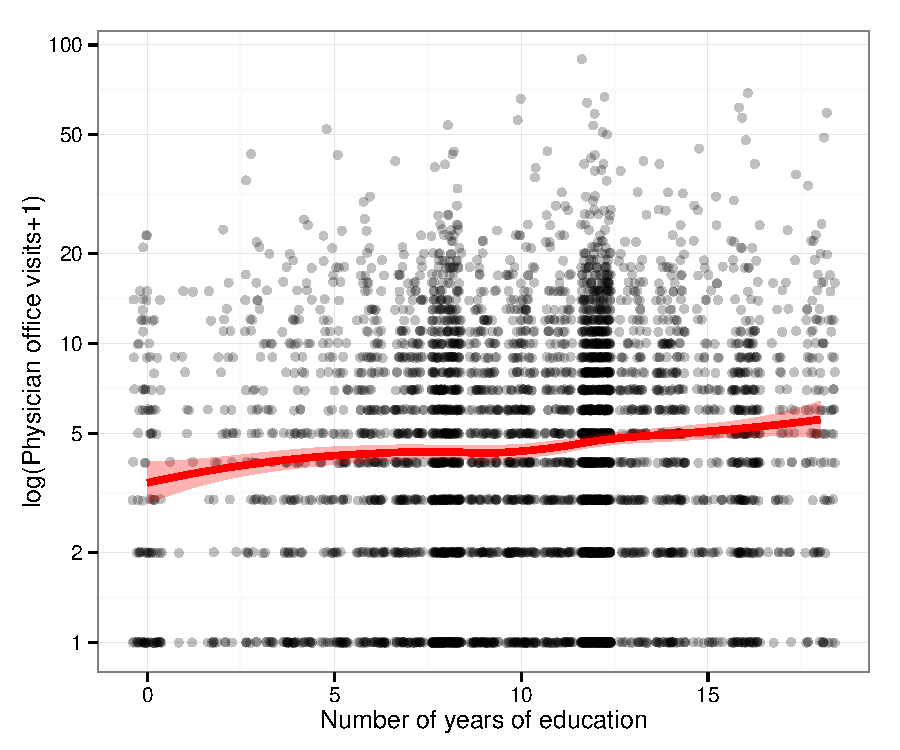
\includegraphics[width=.6\textwidth]{ch09/fig/nmes-school-1} }

\caption[Jittered scatterplot of physician office visits against number of years of education, with nonparametric (loess) smooth]{Jittered scatterplot of physician office visits against number of years of education, with nonparametric (loess) smooth.\label{fig:nmes-school}}
\end{figure}


\end{knitrout}
\noindent As you might expect, there is a small but steady increase in mean office visits with
years of education.  It is somewhat surprising that there are quite a few individuals
with 0 years of education; jittering also shows the greater density of observations at
8 and 12 years.

As in previous examples, a variety of other exploratory plots would be helpful in understanding
the relationships among these variables \emph{jointly}, particularly how office visits depends on
combinations of two (or more) predictors.  Some natural candidates would include
mosaic and doubledecker plots (using \code{cutfac(visits)}), e.g., as in \figref{fig:cod1-mosaic},
and conditional or faceted versions of the boxplots shown in \figref{fig:nmes-boxplots}, each
stratified by one (or more) additional predictors. These activities are left as exercises for
the reader.

\end{Example}

\subsubsection{Fitting models}
Most previous analyses of these data have focused on exploring and comparing different types of
count data regression models.  \citet{DebTrivedi:1997} compared the adequacy of fit of the
negative-binomial, a hurdle NB, and models using finite mixtures of NB models.
\citet{Zeileis-etal:2008} used this data to illustrate hurdle and zero-inflated models using
the \Rpackage{countreg}, while \citet{CameronTrivedi:1998,CameronTrivedi:2013} explored a variety of competing
models, including 1- and 2-parameter NB models and $C$-component finite mixture models
that can be thought of as generalizations of the 2-component models described in \secref{sec:glm-zeros}.

In most cases, the full set of available predictors was used, and models were compared using the
standard methods for model selection: \LR tests for nested models, AIC, BIC and so forth.
An exception is \citet{KleiberZeileis:2014}, who used a reduced set of predictors similar to
those employed here, and illustrated the use of rootograms and plots of predicted values
for visualizing and comparing fitted models.

This is where model comparison and selection for count data models (and other GLMs) adds another
layer of complexity beyond what needs to be considered for classical (Gaussian) linear models,
standard logistic regression models and the special case of \loglin models treated earlier.
Thus, when we consider and compare different distribution types or link functions, we have to
be reasonably confident that the systematic part of the model has been correctly specified
(as we noted in \secref{sec:glm-overdisp}), and is the \emph{same} in all competing models, so that
any differences can be attributed to the distribution type.  However, lack-of-fit may still
arise because the systematic part of the model is incorrect.

In short, we cannot easily compare apples
to oranges (different distributions with different regressors),
but we also have to make sure we have a good apple to begin with. The important questions are:
\begin{itemize*}
  \item Have all important predictors and control variables have been included in the model?
  \item Are quantitative predictors represented on the correct scale (via transformations or non-linear terms)
  so their effects are reasonably additive for the linear predictor?
  \item Are there important interactions among the explanatory variables?
\end{itemize*}


\begin{Example}[nmes2]{Demand for medical care}
In this example, we start with the all main-effects model of the predictors in the \code{nmes}
data, similar to that considered by \citet{Zeileis-etal:2008}.  We first fit the basic Poisson
and NB models, as points of reference.

\begin{knitrout}
\definecolor{shadecolor}{rgb}{1, 0.961, 0.933}\color{fgcolor}\begin{kframe}
\begin{alltt}
\hlstd{nmes.pois}   \hlkwb{<-}      \hlkwd{glm}\hlstd{(visits} \hlopt{~} \hlstd{.,} \hlkwc{data} \hlstd{= nmes,} \hlkwc{family} \hlstd{= poisson)}
\hlstd{nmes.nbin}   \hlkwb{<-}   \hlkwd{glm.nb}\hlstd{(visits} \hlopt{~} \hlstd{.,} \hlkwc{data} \hlstd{= nmes)}
\end{alltt}
\end{kframe}
\end{knitrout}
A quick check with \func{lmtest} shows that the NB model is clearly superior
superior to the standard Poisson regression model as we expect
(and also to the quasi-Poisson).
\begin{knitrout}
\definecolor{shadecolor}{rgb}{1, 0.961, 0.933}\color{fgcolor}\begin{kframe}
\begin{alltt}
\hlkwd{library}\hlstd{(lmtest)}
\hlkwd{lrtest}\hlstd{(nmes.pois, nmes.nbin)}
\end{alltt}
\begin{verbatim}
## Likelihood ratio test
## 
## Model 1: visits ~ hospital + health + chronic + gender + school + insurance
## Model 2: visits ~ hospital + health + chronic + gender + school + insurance
##   #Df LogLik Df Chisq Pr(>Chisq)    
## 1   8 -17972                        
## 2   9 -12171  1 11602     <2e-16 ***
## ---
## Signif. codes:  0 '***' 0.001 '**' 0.01 '*' 0.05 '.' 0.1 ' ' 1
\end{verbatim}
\end{kframe}
\end{knitrout}
The model summary for the NB model below shows the coefficients area all significant.
Moreover, the signs of the coefficients are all as we would expect from our
exploratory plots. For example, log(visits) increases with number of hospital
stays, chronic conditions and education, and is greater for females and
those with private health insurance.  So, what's not to like?
\begin{knitrout}
\definecolor{shadecolor}{rgb}{1, 0.961, 0.933}\color{fgcolor}\begin{kframe}
\begin{alltt}
\hlkwd{summary}\hlstd{(nmes.nbin)}
\end{alltt}
\begin{verbatim}
## 
## Call:
## glm.nb(formula = visits ~ ., data = nmes, init.theta = 1.206603534, 
##     link = log)
## 
## Deviance Residuals: 
##    Min      1Q  Median      3Q     Max  
## -3.047  -0.995  -0.295   0.296   5.818  
## 
## Coefficients:
##                 Estimate Std. Error z value Pr(>|z|)    
## (Intercept)      0.92926    0.05459   17.02  < 2e-16 ***
## hospital         0.21777    0.02018   10.79  < 2e-16 ***
## healthpoor       0.30501    0.04851    6.29  3.2e-10 ***
## healthexcellent -0.34181    0.06092   -5.61  2.0e-08 ***
## chronic          0.17492    0.01209   14.47  < 2e-16 ***
## gendermale      -0.12649    0.03122   -4.05  5.1e-05 ***
## school           0.02682    0.00439    6.10  1.0e-09 ***
## insuranceyes     0.22440    0.03946    5.69  1.3e-08 ***
## ---
## Signif. codes:  0 '***' 0.001 '**' 0.01 '*' 0.05 '.' 0.1 ' ' 1
## 
## (Dispersion parameter for Negative Binomial(1.2066) family taken to be 1)
## 
##     Null deviance: 5743.7  on 4405  degrees of freedom
## Residual deviance: 5044.5  on 4398  degrees of freedom
## AIC: 24359
## 
## Number of Fisher Scoring iterations: 1
## 
## 
##               Theta:  1.2066 
##           Std. Err.:  0.0336 
## 
##  2 x log-likelihood:  -24341.1070
\end{verbatim}
\end{kframe}
\end{knitrout}

This all-main-effects model is relatively
simple to interpret, but a more important question is whether it
adequately explains the relations of the predictors to the outcome,
\var{visits}.

Significant interactions among the predictors could substantially change
the interpretation of the model, and in the end, could affect policy
recommendations based on this analysis. This question turns out to be
far more interesting and important than the subtle differences among
models for handling overdispersion and zero counts.

One simple way to consider whether there are important interactions
among the predictors that better explain patient visits is to get simple
tests of the additional contribution of each two-way (or higher-way)
interaction using the \func{add1} function.  The formula argument in
the call below specifies to test the addition of all two-way terms.

\begin{knitrout}
\definecolor{shadecolor}{rgb}{1, 0.961, 0.933}\color{fgcolor}\begin{kframe}
\begin{alltt}
\hlkwd{add1}\hlstd{(nmes.nbin, .} \hlopt{~} \hlstd{.}\hlopt{^}\hlnum{2}\hlstd{,} \hlkwc{test}\hlstd{=}\hlstr{"Chisq"}\hlstd{)}
\end{alltt}
\begin{verbatim}
## Single term additions
## 
## Model:
## visits ~ hospital + health + chronic + gender + school + insurance
##                    Df Deviance   AIC  LRT Pr(>Chi)    
## <none>                    5045 24357                  
## hospital:health     2     5025 24341 19.9  4.7e-05 ***
## hospital:chronic    1     5009 24324 35.2  3.0e-09 ***
## hospital:gender     1     5044 24358  0.8   0.3650    
## hospital:school     1     5041 24355  4.0   0.0453 *  
## hospital:insurance  1     5036 24351  8.0   0.0046 ** 
## health:chronic      2     5005 24322 39.5  2.6e-09 ***
## health:gender       2     5040 24357  4.3   0.1172    
## health:school       2     5030 24347 14.3   0.0008 ***
## health:insurance    2     5032 24348 12.9   0.0016 ** 
## chronic:gender      1     5045 24359  0.0   0.9008    
## chronic:school      1     5043 24357  1.9   0.1705    
## chronic:insurance   1     5039 24354  5.1   0.0246 *  
## gender:school       1     5040 24354  4.8   0.0290 *  
## gender:insurance    1     5042 24357  2.5   0.1169    
## school:insurance    1     5037 24352  7.2   0.0072 ** 
## ---
## Signif. codes:  0 '***' 0.001 '**' 0.01 '*' 0.05 '.' 0.1 ' ' 1
\end{verbatim}
\end{kframe}
\end{knitrout}
\noindent From this, we decide to add all two-way interactions among
\var{health}, \var{hosp} and \var{numchron}, and also the
two-way interaction \code{health:school}.  Other significant interactions
could also be explored, but we don't do this here.

\begin{knitrout}
\definecolor{shadecolor}{rgb}{1, 0.961, 0.933}\color{fgcolor}\begin{kframe}
\begin{alltt}
\hlstd{nmes.nbin2} \hlkwb{<-} \hlkwd{update}\hlstd{(nmes.nbin,}
                     \hlstd{.} \hlopt{~} \hlstd{.} \hlopt{+} \hlstd{(health}\hlopt{+}\hlstd{chronic}\hlopt{+}\hlstd{hospital)}\hlopt{^}\hlnum{2}
                           \hlopt{+} \hlstd{health}\hlopt{:}\hlstd{school)}
\end{alltt}
\end{kframe}
\end{knitrout}
This model clearly fits much better than the main effects model, as
shown by a likelihood ratio test. The same
conclusion would result from \func{anova}.
\begin{knitrout}
\definecolor{shadecolor}{rgb}{1, 0.961, 0.933}\color{fgcolor}\begin{kframe}
\begin{alltt}
\hlkwd{lrtest}\hlstd{(nmes.nbin, nmes.nbin2)}
\end{alltt}
\begin{verbatim}
## Likelihood ratio test
## 
## Model 1: visits ~ hospital + health + chronic + gender + school + insurance
## Model 2: visits ~ hospital + health + chronic + gender + school + insurance + 
##     health:chronic + hospital:health + hospital:chronic + health:school
##   #Df LogLik Df Chisq Pr(>Chisq)    
## 1   9 -12171                        
## 2  16 -12133  7  74.3      2e-13 ***
## ---
## Signif. codes:  0 '***' 0.001 '**' 0.01 '*' 0.05 '.' 0.1 ' ' 1
\end{verbatim}
\end{kframe}
\end{knitrout}
\end{Example}

\subsubsection{Model interpretation: Effect plots}
Complex models with more than a few predictors are difficult to
understand and explain, even more so when there are interactions among
the predictors. As we have noted previously, effect plots \citep{Fox:87,FoxAndersen:2006}
provide a ready solution.

They have the advantage that each plot shows the correct \emph{partial}
relation between the response and the variables in the term shown,
controlling (adjusting) for all other variables in the model, as opposed
to \emph{marginal} plots that ignore all other variables.
From these, it is possible to read an interpretation of a given model
effect directly from the effect plot graphs, knowing that all variables
not shown in a given graph have been controlled (adjusted for) by setting them
equal to average or typical values.

A disadvantage is that these plots show only the predicted (fitted)
effects under the \emph{given model} (and not the \emph{data}). If relationships of
the response to predictors are nonlinear, or important interactions are
not included in the model, you won't see this in an effect plot.
We illustrate this point using
the results of the main effect NB model,
\code{nmes.nbin}, as shown in \figref{fig:nmes2-eff1}.

\begin{Example}[nmes2a]{Demand for medical care}

\begin{knitrout}
\definecolor{shadecolor}{rgb}{1, 0.961, 0.933}\color{fgcolor}\begin{kframe}
\begin{alltt}
\hlkwd{library}\hlstd{(effects)}
\hlkwd{plot}\hlstd{(}\hlkwd{allEffects}\hlstd{(nmes.nbin),} \hlkwc{ylab} \hlstd{=} \hlstr{"Office visits"}\hlstd{)}
\end{alltt}
\end{kframe}\begin{figure}[!htbp]


\centerline{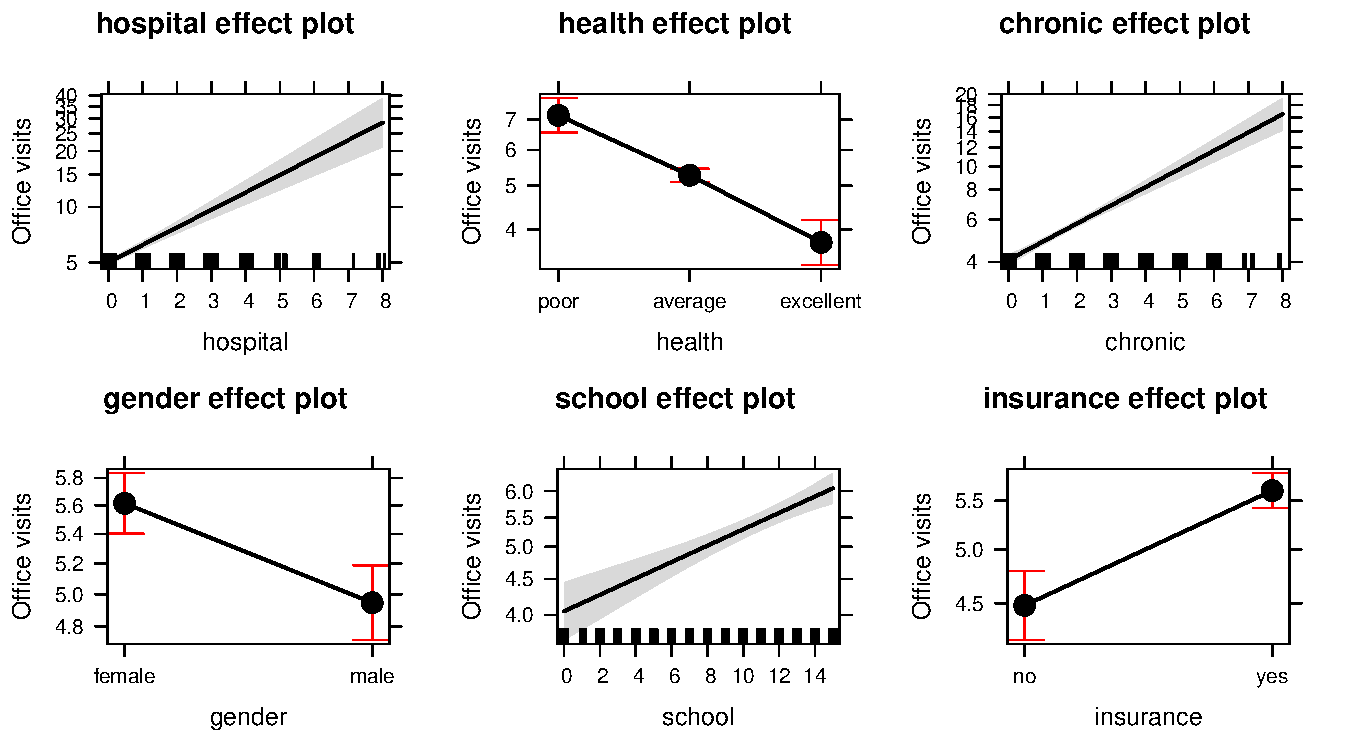
\includegraphics[width=\textwidth]{ch09/fig/nmes2-eff1-1} }

\caption[Effects plots for the main effects of each predictor in the negative binomial model nmes]{Effects plots for the main effects of each predictor in the negative binomial model nmes.nbin\label{fig:nmes2-eff1}}
\end{figure}


\end{knitrout}
All of these panels show the expected relations of the predictors to the
\var{visits} response, and the confidence bands and error bars provide
visual tests of the sizes of differences. But they don't tell the full
story, because the presence of an important interaction (such as \code{health:chronic})
means that the
effect of one predictor (\code{health}) differs over the values of the other (\code{chronic}).

We can see this clearly in effect plots for the model \code{nmes.nbin2} with interactions.
For display purposes,
it is convenient here to calculate the fitted effects for model terms
over a smaller but representative subset of the levels of the
integer-valued predictors, using the \code{xlevels=} argument to
\func{allEffects}.

\begin{knitrout}
\definecolor{shadecolor}{rgb}{1, 0.961, 0.933}\color{fgcolor}\begin{kframe}
\begin{alltt}
\hlstd{eff_nbin2} \hlkwb{<-} \hlkwd{allEffects}\hlstd{(nmes.nbin2,}
  \hlkwc{xlevels}\hlstd{=}\hlkwd{list}\hlstd{(}\hlkwc{hospital}\hlstd{=}\hlkwd{c}\hlstd{(}\hlnum{0}\hlopt{:}\hlnum{3}\hlstd{,} \hlnum{6}\hlstd{,} \hlnum{8}\hlstd{),} \hlkwc{chronic}\hlstd{=}\hlkwd{c}\hlstd{(}\hlnum{0}\hlopt{:}\hlnum{3}\hlstd{,} \hlnum{6}\hlstd{,} \hlnum{8}\hlstd{),} \hlkwc{school}\hlstd{=}\hlkwd{seq}\hlstd{(}\hlnum{0}\hlstd{,}\hlnum{20}\hlstd{,}\hlnum{5}\hlstd{)))}
\end{alltt}
\end{kframe}
\end{knitrout}
The result of \func{allEffects}, \code{eff\_nbin2}, is a \class{efflist} object, a list of effects for each
\emph{high-order term} in the model.  Note that only the terms \code{gender} and \code{insurance},
not involved in any interaction, appear as main effects here.
\begin{knitrout}
\definecolor{shadecolor}{rgb}{1, 0.961, 0.933}\color{fgcolor}\begin{kframe}
\begin{alltt}
\hlkwd{names}\hlstd{(eff_nbin2)}
\end{alltt}
\begin{verbatim}
## [1] "gender"           "insurance"        "health:chronic"  
## [4] "hospital:health"  "hospital:chronic" "health:school"
\end{verbatim}
\end{kframe}
\end{knitrout}
Plotting the entire \class{efflist} object gives a collection of plots, one for each high-order term, as in
\figref{fig:nmes2-eff1}, and is handy for a first look. However, the \func{plot} methods for effects
objects offer greater flexibility when you plot terms individually using additional options.
For example, \figref{fig:nmes2-eff2} plots the effect for the interaction of health and number of chronic conditions
with a few optional arguments. See \help{plot.eff, package="effects"} for the available options.

\begin{knitrout}
\definecolor{shadecolor}{rgb}{1, 0.961, 0.933}\color{fgcolor}\begin{kframe}
\begin{alltt}
\hlkwd{plot}\hlstd{(eff_nbin2,} \hlstr{"health:chronic"}\hlstd{,} \hlkwc{layout}\hlstd{=}\hlkwd{c}\hlstd{(}\hlnum{3}\hlstd{,}\hlnum{1}\hlstd{),}
     \hlkwc{ylab} \hlstd{=} \hlstr{"Office visits"}\hlstd{,} \hlkwc{colors}\hlstd{=}\hlstr{"blue"}\hlstd{)}
\end{alltt}
\end{kframe}\begin{figure}[!htbp]


\centerline{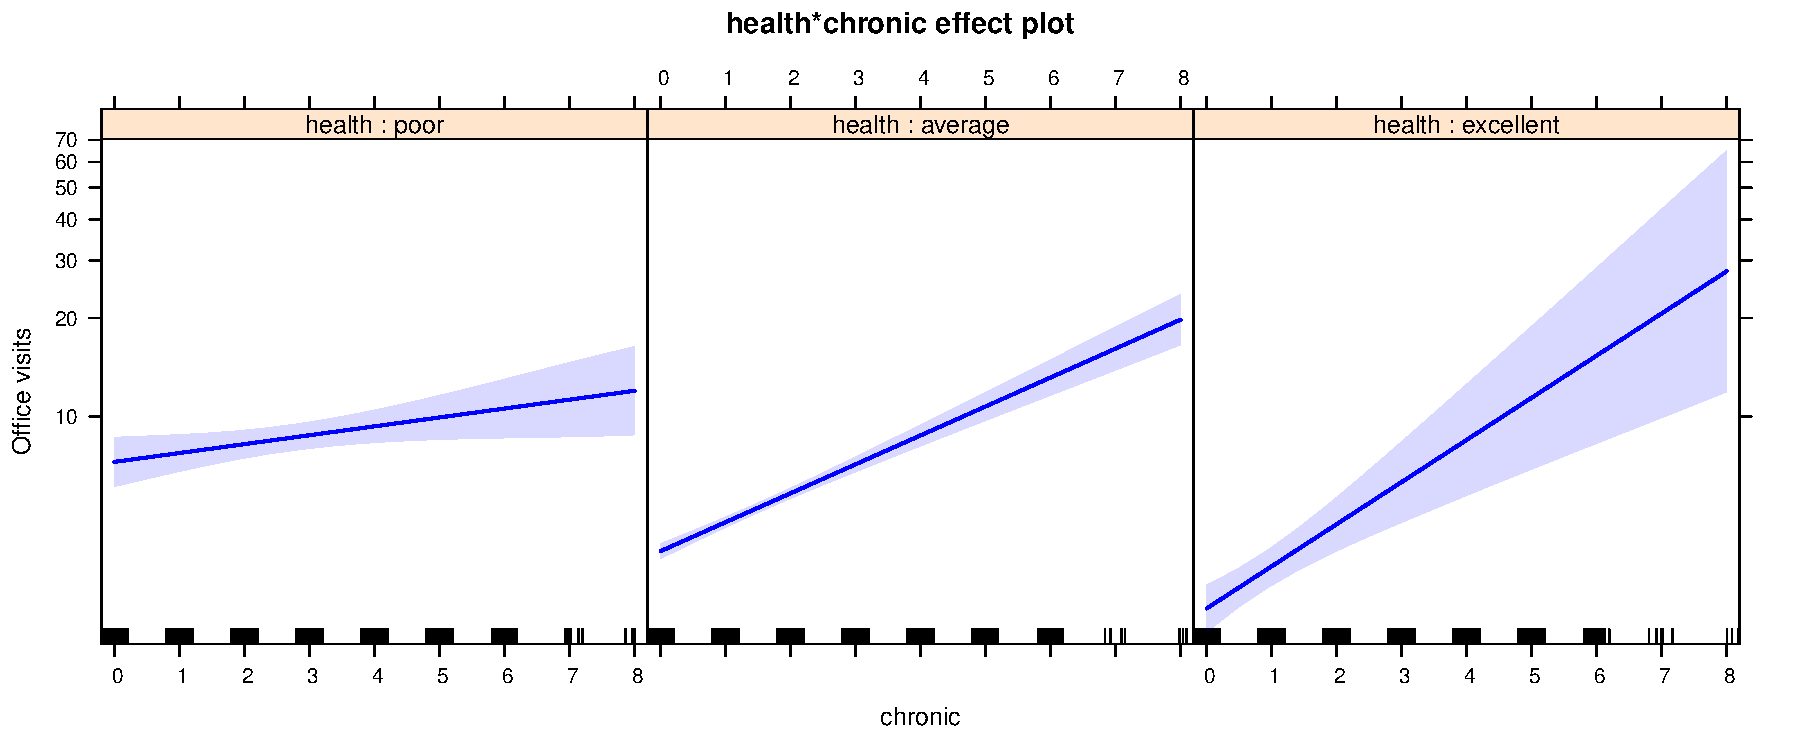
\includegraphics[width=\textwidth]{ch09/fig/nmes2-eff2-1} }

\caption[Effect plot for the interaction of health and number of chronic conditions in the model nmes]{Effect plot for the interaction of health and number of chronic conditions in the model nmes.nbin2\label{fig:nmes2-eff2}}
\end{figure}


\end{knitrout}
The default style shown in \figref{fig:nmes2-eff2}
is a conditional or faceted plot,
graphing the response against the X variable with the greatest number of levels,
with separate panels for the levels of the other predictor.
Alternatively, the effects for a given term
can be shown overlaid in a single plot, using
the \code{multiline=TRUE} argument, as shown in \figref{fig:nmes2-eff3} for the two interactions involving health status.
Not only is this style more compact, but it also makes direct comparison of the trends for the other variable easier.


\begin{knitrout}
\definecolor{shadecolor}{rgb}{1, 0.961, 0.933}\color{fgcolor}\begin{kframe}
\begin{alltt}
\hlkwd{plot}\hlstd{(eff_nbin2,} \hlstr{"health:chronic"}\hlstd{,} \hlkwc{multiline}\hlstd{=}\hlnum{TRUE}\hlstd{,} \hlkwc{ci.style}\hlstd{=}\hlstr{"bands"}\hlstd{,}
     \hlkwc{ylab} \hlstd{=} \hlstr{"Office visits"}\hlstd{,} \hlkwc{xlab}\hlstd{=}\hlstr{"# Chronic conditions"}\hlstd{,}
     \hlkwc{key.args} \hlstd{=} \hlkwd{list}\hlstd{(}\hlkwc{x} \hlstd{=} \hlnum{0.05}\hlstd{,} \hlkwc{y} \hlstd{=} \hlnum{.80}\hlstd{,} \hlkwc{corner} \hlstd{=} \hlkwd{c}\hlstd{(}\hlnum{0}\hlstd{,} \hlnum{0}\hlstd{)))}

\hlkwd{plot}\hlstd{(eff_nbin2,} \hlstr{"hospital:health"}\hlstd{,} \hlkwc{multiline}\hlstd{=}\hlnum{TRUE}\hlstd{,} \hlkwc{ci.style}\hlstd{=}\hlstr{"bands"}\hlstd{,}
     \hlkwc{ylab} \hlstd{=} \hlstr{"Office visits"}\hlstd{,} \hlkwc{xlab}\hlstd{=}\hlstr{"Hospital stays"}\hlstd{,}
     \hlkwc{key.args} \hlstd{=} \hlkwd{list}\hlstd{(}\hlkwc{x} \hlstd{=} \hlnum{0.05}\hlstd{,} \hlkwc{y} \hlstd{=} \hlnum{.80}\hlstd{,} \hlkwc{corner} \hlstd{=} \hlkwd{c}\hlstd{(}\hlnum{0}\hlstd{,} \hlnum{0}\hlstd{)))}
\end{alltt}
\end{kframe}\begin{figure}[!htbp]


\centerline{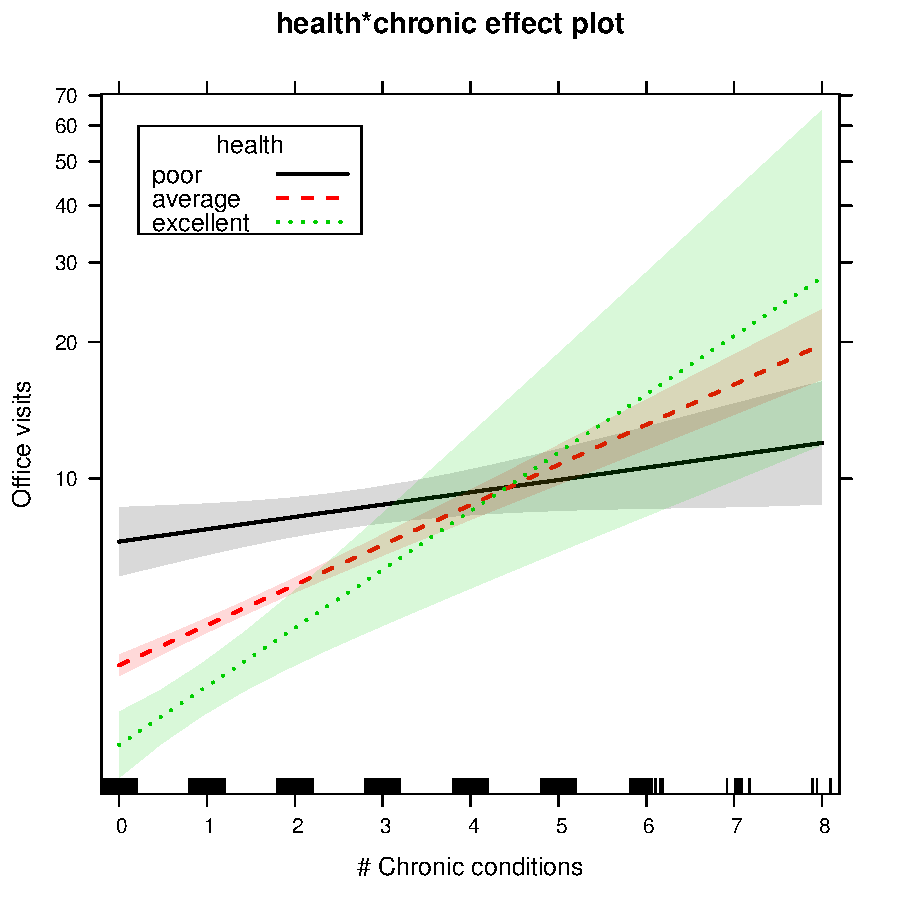
\includegraphics[width=.49\textwidth]{ch09/fig/nmes2-eff3-1} 
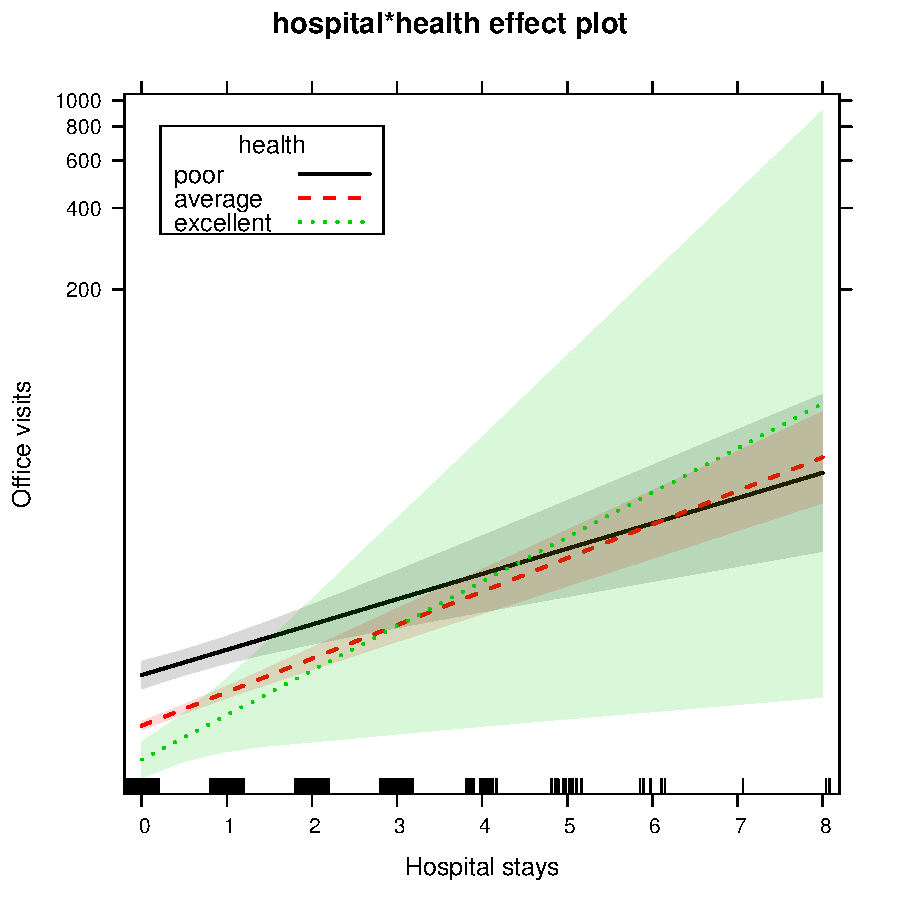
\includegraphics[width=.49\textwidth]{ch09/fig/nmes2-eff3-2} }

\caption[Effect plots for the interactions of chronic conditions and hospital stays with perceived health status in the model nmes]{Effect plots for the interactions of chronic conditions and hospital stays with perceived health status in the model nmes.nbin2\label{fig:nmes2-eff3}}
\end{figure}


\end{knitrout}

From both \figref{fig:nmes2-eff2} and the left panel of
and \figref{fig:nmes2-eff3}, it can be seen that for people with poor health
status, the relationship of chronic conditions to office visits is
relatively flat. For those who view their health status as excellent,
their use of office visits is much more strongly related to their number
of chronic conditions.

The interaction of perceived health status with number of
hospital stays (right panel of \figref{fig:nmes2-eff3}) shows that
the difference in office visits according to health status is mainly
important only for those with 0 or 1 hospital stays.

The remaining two interaction effects are plotted in \figref{fig:nmes2-eff4}.
The interaction of hospital stays and number of chronic
conditions (left panel of \figref{fig:nmes2-eff4})
has a clearly interpretable pattern: for those with few
chronic conditions, there is a strong positive relationship between
hospital stays and office visits. As the number of chronic conditions
increases, the relation with hospital stays decreases in slope.

\begin{knitrout}
\definecolor{shadecolor}{rgb}{1, 0.961, 0.933}\color{fgcolor}\begin{kframe}
\begin{alltt}
\hlkwd{plot}\hlstd{(eff_nbin2,} \hlstr{"hospital:chronic"}\hlstd{,} \hlkwc{multiline}\hlstd{=}\hlnum{TRUE}\hlstd{,} \hlkwc{ci.style}\hlstd{=}\hlstr{"bands"}\hlstd{,}
     \hlkwc{ylab} \hlstd{=} \hlstr{"Office visits"}\hlstd{,} \hlkwc{xlab}\hlstd{=}\hlstr{"Hospital stays"}\hlstd{,}
     \hlkwc{key.args} \hlstd{=} \hlkwd{list}\hlstd{(}\hlkwc{x} \hlstd{=} \hlnum{0.05}\hlstd{,} \hlkwc{y} \hlstd{=} \hlnum{.70}\hlstd{,} \hlkwc{corner} \hlstd{=} \hlkwd{c}\hlstd{(}\hlnum{0}\hlstd{,} \hlnum{0}\hlstd{)))}

\hlkwd{plot}\hlstd{(eff_nbin2,} \hlstr{"health:school"}\hlstd{,} \hlkwc{multiline}\hlstd{=}\hlnum{TRUE}\hlstd{,}  \hlkwc{ci.style}\hlstd{=}\hlstr{"bands"}\hlstd{,}
     \hlkwc{ylab} \hlstd{=} \hlstr{"Office visits"}\hlstd{,} \hlkwc{xlab}\hlstd{=}\hlstr{"Years of education"}\hlstd{,}
     \hlkwc{key.args} \hlstd{=} \hlkwd{list}\hlstd{(}\hlkwc{x} \hlstd{=} \hlnum{0.65}\hlstd{,} \hlkwc{y} \hlstd{=} \hlnum{.1}\hlstd{,} \hlkwc{corner} \hlstd{=} \hlkwd{c}\hlstd{(}\hlnum{0}\hlstd{,} \hlnum{0}\hlstd{)))}
\end{alltt}
\end{kframe}\begin{figure}[!htbp]


\centerline{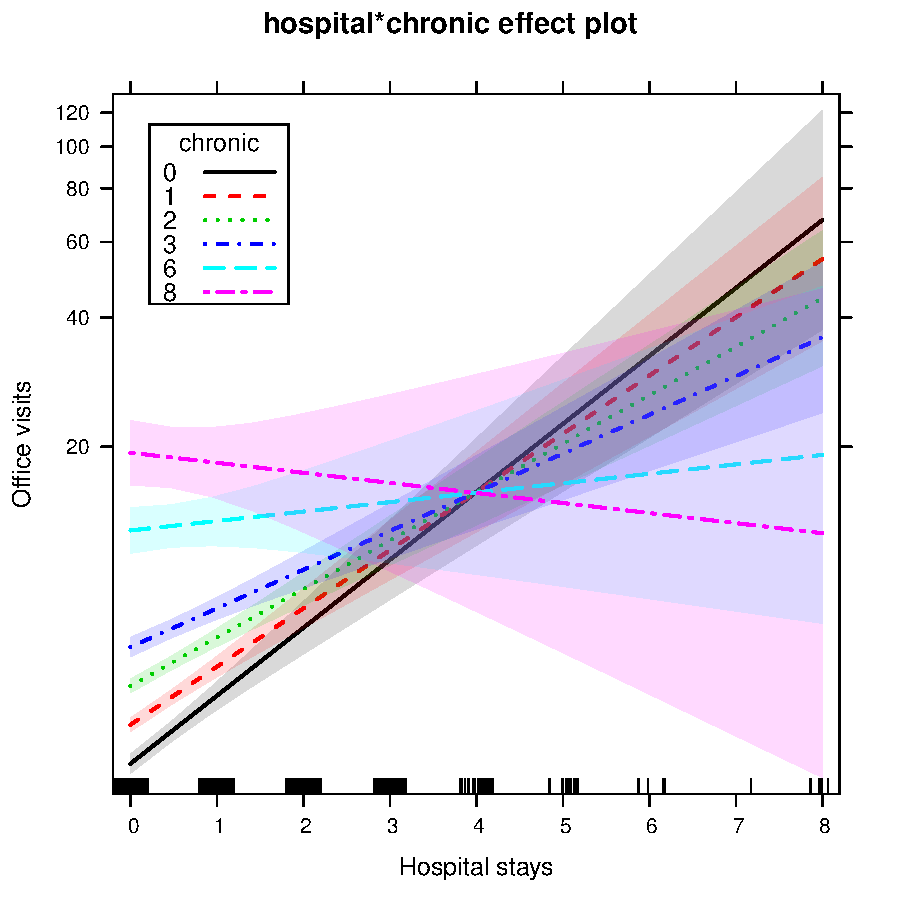
\includegraphics[width=.49\textwidth]{ch09/fig/nmes2-eff4-1} 
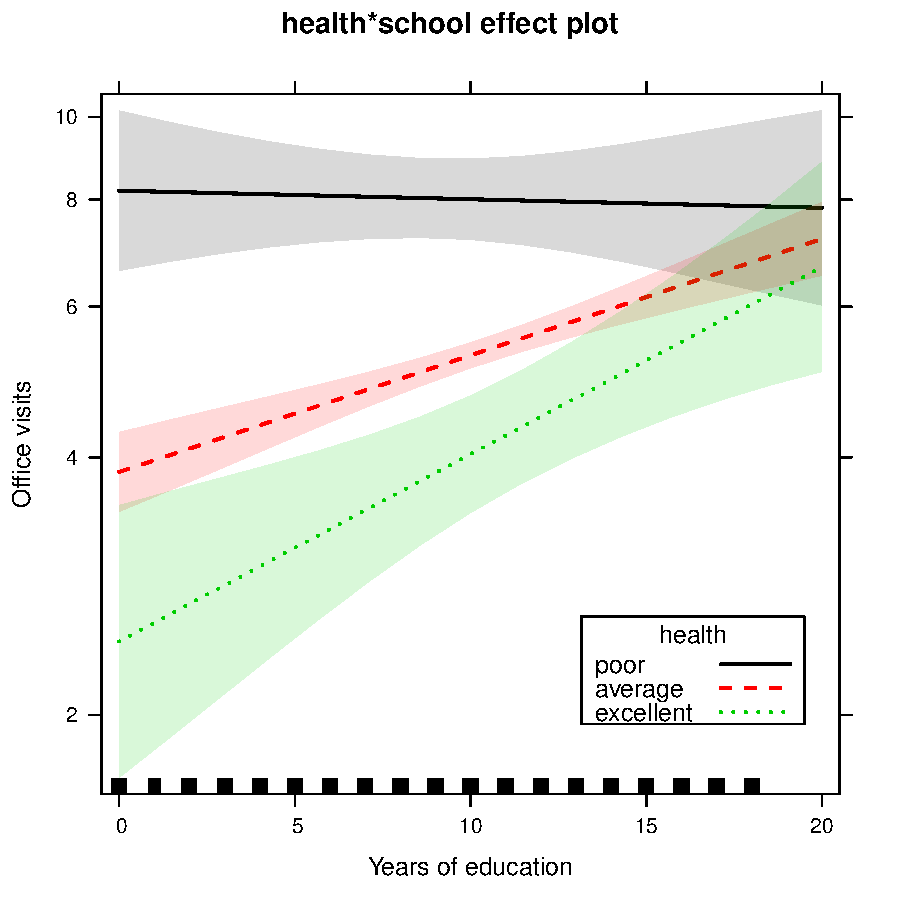
\includegraphics[width=.49\textwidth]{ch09/fig/nmes2-eff4-2} }

\caption[Effect plots for the interactions of chronic conditions and hospital stays and for health status with years of education in the model nmes]{Effect plots for the interactions of chronic conditions and hospital stays and for health status with years of education in the model nmes.nbin2\label{fig:nmes2-eff4}}
\end{figure}


\end{knitrout}

Finally, the interaction of \code{health:school} is shown in the right panel of
\figref{fig:nmes2-eff4}. It
can be readily seen that for those of poor health, office visits are
uniformly high, and have no relation to years of education. Among
those of average or excellent health, office visits increase with years
of education in roughly similar ways.
\end{Example}

\subsubsection{More model wrinkles: Nonlinear terms}

Effect plots such as those above are much easier to interpret than
tables of fitted coefficients. However, we emphasize that these only
reflect the \emph{fitted model}. It might be that the effects of both
\var{hospital} and \var{chronic} are nonlinear (on the scale of
\code{log(visits)}).
In assessing this question, we increase the complexity of model
and try to balance parsimony against goodness-of-fit, but also assure
that the model retains a sensible interpretation.

\begin{Example}[nmes3]{Demand for medical care}

The simplest approach is to use
\code{poly(hosp,2)} and/or \code{poly(numchron,2)} to add
possible quadratic (or higher power) relations to the model \code{nmes.nbin2}
containing interactions studied above.
A slightly more
complex model could use \code{poly(hosp, numchron, degree=2)}
for a response-surface model in these variables.
A significantly improved fit of such a model is evidence for nonlinearity of the effects
of these predictors.  This is easily done using \func{update}:
\begin{knitrout}
\definecolor{shadecolor}{rgb}{1, 0.961, 0.933}\color{fgcolor}\begin{kframe}
\begin{alltt}
\hlstd{nmes.nbin3} \hlkwb{<-} \hlkwd{update}\hlstd{(nmes.nbin2, .} \hlopt{~} \hlstd{.} \hlopt{+} \hlkwd{I}\hlstd{(chronic}\hlopt{^}\hlnum{2}\hlstd{)} \hlopt{+} \hlkwd{I}\hlstd{(hospital}\hlopt{^}\hlnum{2}\hlstd{))}
\end{alltt}
\end{kframe}
\end{knitrout}
\noindent This model is equivalent to the long-form version below:
\begin{knitrout}
\definecolor{shadecolor}{rgb}{1, 0.961, 0.933}\color{fgcolor}\begin{kframe}
\begin{alltt}
\hlstd{nmes.nbin3} \hlkwb{<-} \hlkwd{glm.nb}\hlstd{(visits} \hlopt{~} \hlkwd{poly}\hlstd{(hospital,}\hlnum{2}\hlstd{)} \hlopt{+} \hlkwd{poly}\hlstd{(chronic,}\hlnum{2}\hlstd{)} \hlopt{+}
                     \hlstd{insurance} \hlopt{+} \hlstd{school} \hlopt{+} \hlstd{gender} \hlopt{+}
                     \hlstd{(health}\hlopt{+}\hlstd{chronic}\hlopt{+}\hlstd{hospital)}\hlopt{^}\hlnum{2} \hlopt{+} \hlstd{health}\hlopt{:}\hlstd{school,} \hlkwc{data} \hlstd{= nmes)}
\end{alltt}
\end{kframe}
\end{knitrout}
Comparing these models using \func{anova}, we see that there is a substantial improvement in the
model fit by including these nonlinear terms.  The quadratic model also fits best by AIC and BIC.
\begin{knitrout}
\definecolor{shadecolor}{rgb}{1, 0.961, 0.933}\color{fgcolor}\begin{kframe}
\begin{alltt}
\hlkwd{anova}\hlstd{(nmes.nbin, nmes.nbin2, nmes.nbin3)}
\end{alltt}
\begin{verbatim}
## Likelihood ratio tests of Negative Binomial Models
## 
## Response: visits
##                                                                                                                                                            Model
## 1                                                                                                      hospital + health + chronic + gender + school + insurance
## 2                                hospital + health + chronic + gender + school + insurance + health:chronic + hospital:health + hospital:chronic + health:school
## 3 hospital + health + chronic + gender + school + insurance + I(chronic^2) + I(hospital^2) + health:chronic + hospital:health + hospital:chronic + health:school
##    theta Resid. df    2 x log-lik.   Test    df LR stat.
## 1 1.2066      4398          -24341                      
## 2 1.2354      4391          -24267 1 vs 2     7   74.307
## 3 1.2446      4389          -24245 2 vs 3     2   22.278
##      Pr(Chi)
## 1           
## 2 1.9829e-13
## 3 1.4537e-05
\end{verbatim}
\begin{alltt}
\hlstd{vcdExtra::}\hlkwd{Summarise}\hlstd{(nmes.nbin, nmes.nbin2, nmes.nbin3)}
\end{alltt}
\begin{verbatim}
## Likelihood summary table:
##              AIC   BIC LR Chisq   Df Pr(>Chisq)    
## nmes.nbin  24359 24417     5045 4398    2.2e-11 ***
## nmes.nbin2 24299 24401     5047 4391    1.1e-11 ***
## nmes.nbin3 24281 24396     5049 4389    8.5e-12 ***
## ---
## Signif. codes:  0 '***' 0.001 '**' 0.01 '*' 0.05 '.' 0.1 ' ' 1
\end{verbatim}
\end{kframe}
\end{knitrout}
However, effect plots for this model quickly reveal a \emph{substantive} limitation of this approach using polynomial terms.
\figref{fig:nmes3-eff1} shows one such plot for the interaction of health and number of chronic conditions
that you should compare with \figref{fig:nmes2-eff2}.
\begin{knitrout}
\definecolor{shadecolor}{rgb}{1, 0.961, 0.933}\color{fgcolor}\begin{kframe}
\begin{alltt}
\hlstd{eff_nbin3} \hlkwb{<-} \hlkwd{allEffects}\hlstd{(nmes.nbin3,}
  \hlkwc{xlevels}\hlstd{=}\hlkwd{list}\hlstd{(}\hlkwc{hospital}\hlstd{=}\hlkwd{c}\hlstd{(}\hlnum{0}\hlopt{:}\hlnum{3}\hlstd{,} \hlnum{6}\hlstd{,} \hlnum{8}\hlstd{),} \hlkwc{chronic}\hlstd{=}\hlkwd{c}\hlstd{(}\hlnum{0}\hlopt{:}\hlnum{3}\hlstd{,} \hlnum{6}\hlstd{,} \hlnum{8}\hlstd{),} \hlkwc{school}\hlstd{=}\hlkwd{seq}\hlstd{(}\hlnum{0}\hlstd{,}\hlnum{20}\hlstd{,}\hlnum{5}\hlstd{)))}
\hlkwd{plot}\hlstd{(eff_nbin3,} \hlstr{"health:chronic"}\hlstd{,} \hlkwc{layout}\hlstd{=}\hlkwd{c}\hlstd{(}\hlnum{3}\hlstd{,}\hlnum{1}\hlstd{))}
\end{alltt}
\end{kframe}\begin{figure}[!htbp]


\centerline{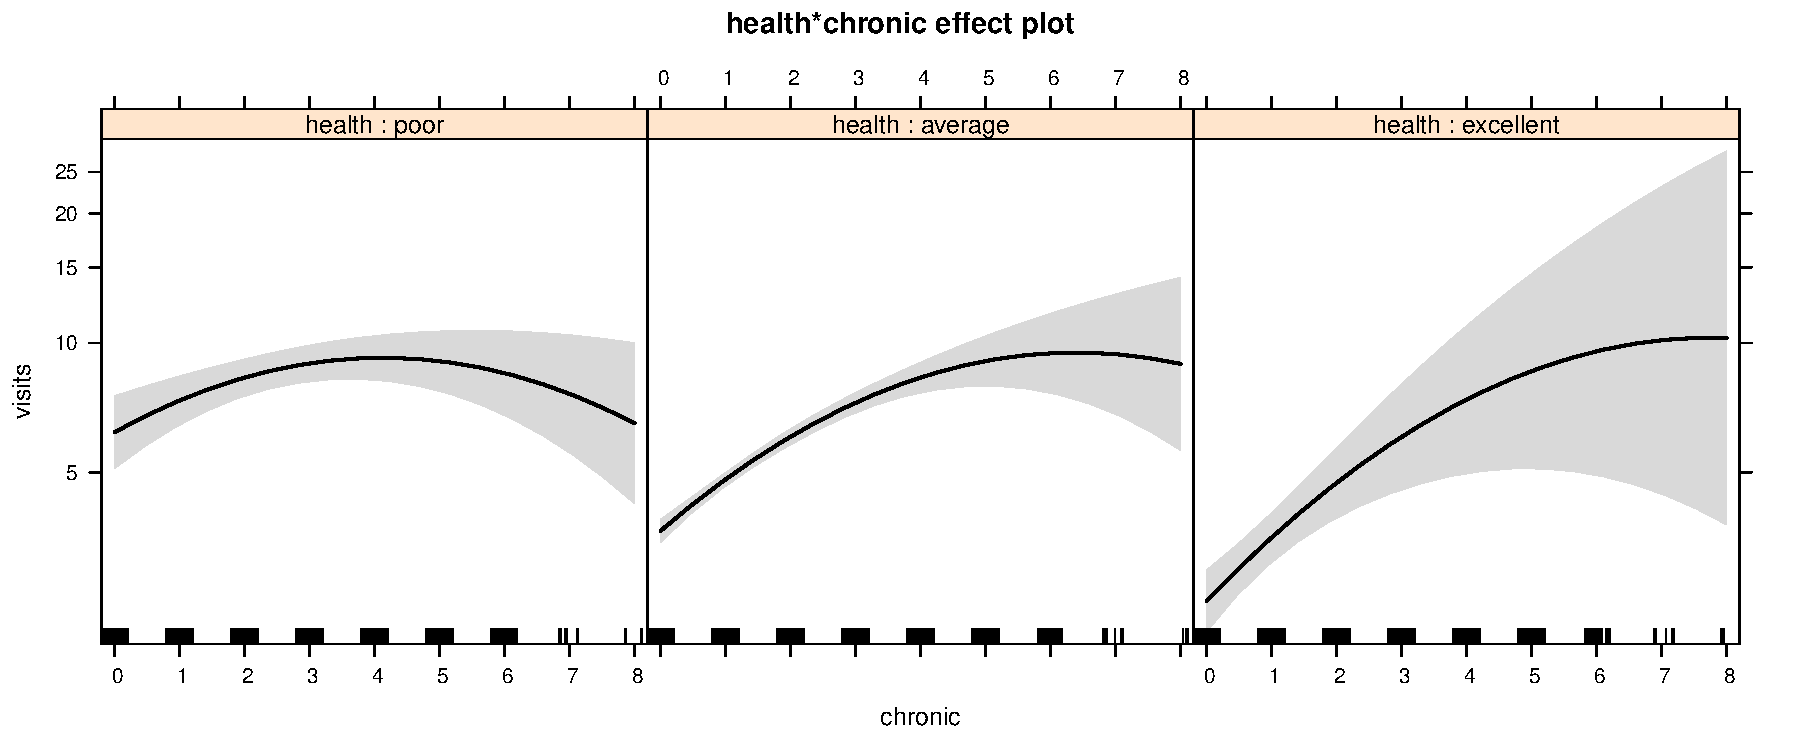
\includegraphics[width=\textwidth]{ch09/fig/nmes3-eff1-1} }

\caption[Effect plot for the interaction of health and number of chronic conditions in the quadratic model nmes]{Effect plot for the interaction of health and number of chronic conditions in the quadratic model nmes.nbin3\label{fig:nmes3-eff1}}
\end{figure}


\end{knitrout}
\noindent The quadratic fits for each level of health in \figref{fig:nmes3-eff1} imply that
office visits increase with chronic conditions up to a point and then decrease---
with a quadratic, what goes up must come down, the same way it went up!  This makes no sense here,
particularly for those with poor health status.  As well, the confidence bands in this figure
are uncomfortably wide, particularly at higher levels of chronic conditions, compared to those
in \figref{fig:nmes2-eff2}.
The quadratic model is thus preferable statistically and descriptively, but serves less well
for explanatory, substantive and predictive goals.

An alternative approach nonlinearity is to use
regression splines
(as in \exref{ex:donner1}) or a \term{generalized additive model} \citep{HastieTibshirani:1990}
for these terms.  The latter specifies the linear predictor as a sum of
smooth functions,
\begin{equation*}
g(\E(y))=\beta_0 + f_1(x_1) + f_2(x_2)+ \cdots + f_m(x_m) \period
\end{equation*}
where each $f_j(x_j)$
may be a function with a specified parametric form (for example a polynomial)
or may be specified non-parametrically, simply as ``smooth functions'', to be estimated by non-parametric means.

In \R, a very general implementation of the generalized additive model (GAM) is provided by
\func{gam} in the \Rpackage{mgcv} and described in detail by \citet{Wood:2006}.
Particular features of the package are facilities for automatic smoothness selection \citep{Wood:2004},
and the provision of a variety of smooths of more than one variable. This example just
scratches the surface of GAM methodology.

In the context of the NB model we are considering here, the analog of model \code{nmes.nbin3}
fitted using \func{gam} is \code{nmes.gamnb} shown below.  The negative-binomial distribution
can be specified using \code{family=nb()} when the parameter $\theta$ is also estimated from
the data (as with \func{glm.nb}), or \code{family=negbin(theta)} when $\theta$ is taken as
fixed,
%(similar to \code{family=negative.binomial(theta)} in \pkg{MASS}),
for example using
the value \code{theta=1.24} available from models \code{nmes.nbin2}, and \code{nmes.nbin3}.
\begin{knitrout}
\definecolor{shadecolor}{rgb}{1, 0.961, 0.933}\color{fgcolor}\begin{kframe}
\begin{alltt}
\hlkwd{library}\hlstd{(mgcv)}
\hlstd{nmes.gamnb} \hlkwb{<-} \hlkwd{gam}\hlstd{(visits} \hlopt{~} \hlkwd{s}\hlstd{(hospital,} \hlkwc{k}\hlstd{=}\hlnum{3}\hlstd{)} \hlopt{+} \hlkwd{s}\hlstd{(chronic,} \hlkwc{k}\hlstd{=}\hlnum{3}\hlstd{)} \hlopt{+}
                           \hlstd{insurance} \hlopt{+} \hlstd{school} \hlopt{+} \hlstd{gender} \hlopt{+}
                           \hlstd{(health}\hlopt{+}\hlstd{chronic}\hlopt{+}\hlstd{hospital)}\hlopt{^}\hlnum{2} \hlopt{+} \hlstd{health}\hlopt{:}\hlstd{school,}
                  \hlkwc{family}\hlstd{=}\hlkwd{nb}\hlstd{(),} \hlkwc{data} \hlstd{= nmes)}
\end{alltt}
\end{kframe}
\end{knitrout}
The key feature here is the specification of the smooth terms for \code{s(hospital, k=3)}
and \code{s(chronic, k=3)}, where \code{k=3} specifies
the dimension of the basis used to represent the smooth term.  There are many other
possibilities with \func{gam}, but these are beyond the scope of this example.

We could again visualize the predicted values from this model using effect plots. However a
different approach is to visualize the \emph{fitted surface} in 3D, using a range of
values for two of the predictors, and controlling for the others.

The \pkg{rsm} package provides extensions of the standard \func{contour}, \func{image}
and \func{persp} functions for this purpose.  The package provides S3 methods
(e.g., \func{persp.lm}) for
\class{lm} objects, or classes (such as \class{negbin} and \class{glm})
that inherit methods from \code{lm}.  The calculation of fitted values in these
plots use the applicable \func{predict} method for the model object.
As in effect plots, the remaining predictors are controlled at their average
values (or other values specified in the \code{at} argument).

Two such plots are shown in \figref{fig:nmes3-rsm}. The left panel shows the interaction of
hospital stays and chronic conditions, included in the model with smoothed terms for their
main effects.  The right panel shows the joint effects of years of education and chronic
conditions on office visits, but there is no interaction of these variables in the GAM model
\code{nmes.gamnb}.
These plots use \func{rainbow} colors to depict the predicted values of office visits.
Contours of these values are projected into the bottom or top plane with corresponding
color coding.%
\footnote{The vignette \code{vignette("rsm-plots", package="rsm")} illustrates some of these options.
}
\begin{knitrout}
\definecolor{shadecolor}{rgb}{1, 0.961, 0.933}\color{fgcolor}\begin{kframe}
\begin{alltt}
\hlkwd{library}\hlstd{(rsm)}
\hlkwd{persp}\hlstd{(nmes.gamnb, hospital} \hlopt{~} \hlstd{chronic,} \hlkwc{zlab}\hlstd{=}\hlstr{"log Office visits"}\hlstd{,}
  \hlkwc{col}\hlstd{=}\hlkwd{rainbow}\hlstd{(}\hlnum{30}\hlstd{),} \hlkwc{contour}\hlstd{=}\hlkwd{list}\hlstd{(}\hlkwc{col}\hlstd{=}\hlstr{"colors"}\hlstd{,} \hlkwc{lwd}\hlstd{=}\hlnum{2}\hlstd{),}
  \hlkwc{at}\hlstd{=}\hlkwd{list}\hlstd{(}\hlkwc{school}\hlstd{=}\hlnum{10}\hlstd{,} \hlkwc{health}\hlstd{=}\hlstr{'average'}\hlstd{),} \hlkwc{theta}\hlstd{=}\hlopt{-}\hlnum{60}\hlstd{)}

\hlkwd{persp}\hlstd{(nmes.gamnb, school} \hlopt{~} \hlstd{chronic,} \hlkwc{zlab}\hlstd{=}\hlstr{"log Office visits"}\hlstd{,}
        \hlkwc{col}\hlstd{=}\hlkwd{rainbow}\hlstd{(}\hlnum{30}\hlstd{),} \hlkwc{contour}\hlstd{=}\hlkwd{list}\hlstd{(}\hlkwc{col}\hlstd{=}\hlstr{"colors"}\hlstd{,} \hlkwc{lwd}\hlstd{=}\hlnum{2}\hlstd{,} \hlkwc{z}\hlstd{=}\hlstr{"top"}\hlstd{),}
  \hlkwc{at}\hlstd{=}\hlkwd{list}\hlstd{(}\hlkwc{hospital}\hlstd{=}\hlnum{0.3}\hlstd{,} \hlkwc{health}\hlstd{=}\hlstr{'average'}\hlstd{),} \hlkwc{theta}\hlstd{=}\hlopt{-}\hlnum{60}\hlstd{)}
\end{alltt}
\end{kframe}\begin{figure}[!htbp]


\centerline{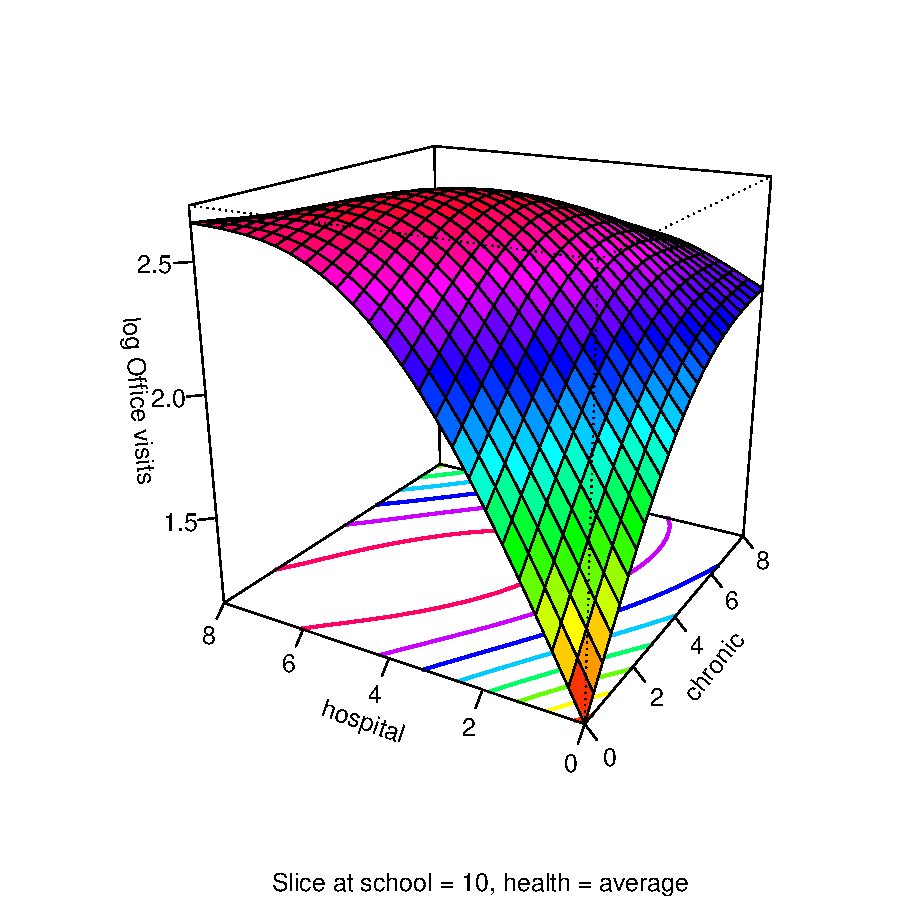
\includegraphics[width=.5\textwidth]{ch09/fig/nmes3-rsm-1} 
\includegraphics[width=.5\textwidth]{ch09/fig/nmes3-rsm-2} }

\caption[Fitted response surfaces for the relationships among chronic conditions,  number of hospital stays and years of education to office visits in the generalized additive model, nmes]{Fitted response surfaces for the relationships among chronic conditions,  number of hospital stays and years of education to office visits in the generalized additive model, nmes.gamnb\label{fig:nmes3-rsm}}
\end{figure}


\end{knitrout}
A simple, credible interpretation of the plot in the left panel is
that office visits rise steeply initially with both hospital stays and number of chronic conditions, and then
levels off. For those with no chronic conditions, the effect of hospital stays rises to a higher level
compared with the effect of chronic conditions among those who have had no hospital stays.
However, as we have seen before, the data is quite thin at the upper end of these
predictors, and this plot does not show model uncertainty.

The right panel of \figref{fig:nmes3-rsm} illustrates the form of model predictions for a term
where one variable (\var{chronic}) is treated as possibly nonlinear using a smooth \func{s}
effect, the other is treated as linear (\var{school}), and no interaction between these is
included in the model.  At each fixed value of \code{chronic}, increasing education results in
greater office visits.  At each fixed value of \code{school}, the number of chronic conditions shows
a steep increase in office visits initially, leveling off toward higher levels, but these all have
the same predicted shape.


\end{Example}



\section{Diagnostic plots for model checking}\label{sec:glm-diag}

\epigraph{Models, of course, are never true, but fortunately it is only necessary that they be useful.}{G. E. P. Box,
\emph{Some Problems of Statistics of Everyday Life}, \citeyear{Box:1979}, p. 2}

Most of the model diagnostic methods for classical linear models extend in a relatively direct way
to GLMs.
These include
\begin{seriate}
  \item plots of residuals of various types,
  \item diagnostic measures and plots of leverage and influence,
as well as some
  \item more specialized plots (component-plus-residual plots, added-variable plots)
designed to show the specific contribution of a given predictor among others in a linear model.
\end{seriate}
These methods were described in \secref{sec:logist-infl} in the context of logistic regression,
and most of that discussion is applicable here in wider GLM class.

One additional complication here is that in any GLM we are specifying:
\begin{seriate}
  \item the distribution of the random component, which for count data models may also involve a dispersion
  parameter or other additional parameters;
  \item the form of the linear predictor, $\eta = \vec{x}\trans \beta = \beta_0 + \beta_1 x_1 + \cdots$,
  where all important regressors have been included, and on the right scale;
  \item the correct link function, $g(\mu) = \eta$
  transforming the conditional mean of the response $y$ to the predictor variables where they have linear
  relationships.
\end{seriate}

Thus, there are a lot of things that could go wrong, but the famous quote from George Box should remind us
that all models are approximate, and the goal for model diagnosis should be an adequate model, useful
for description, estimation or prediction as the case may be. What is most important is that our models
cannot be misleadingly wrong, that is they should not affect substantive conclusions or interpretation.

\subsection{Diagnostic measures and residuals for GLMs}

Estimation of GLMs by maximum likelihood uses an iterative weighted least squares (IWLS) algorithm,
and many of the diagnostic measures for these models are close counterparts of their forms for
classical linear models.  Roughly speaking, these follow from replacing
$\vec{y}$ and $\widehat{\vec{y}}$ in least squares diagnostics by a ``working response'' and
$\widehat{\vec{\eta}}$, replacing the residual variance $\widehat{\sigma}^2$ by $\widehat{\phi}$,
and using a weighted form of the Hat matrix.

\subsubsection{Leverage}
Hat values, $h_i$, measuring leverage or the potential of an observation to affect the fitted model
are defined as the diagonal elements of the hat matrix $\mat{H}$, using the weight matrix
$\mat{W}$ from the final IWLS iteration.  This has the same form as in a weighted least squares
regression using a fixed $\mat{W}$ matrix:
\begin{equation*}
\mat{H} = \mat{W}^{1/2} \mat{X} (\mat{X}\trans \mat{W}  \mat{X} )^{-1} \mat{X}\trans \mat{W}^{1/2} \period
\end{equation*}
In contrast to OLS, the weights depend on the $\vec{y}$ values as well as the $\mat{X}$ values, so
high leverage observations do not necessarily reflect only unusualness in the space of the
predictors.

\subsubsection{Residuals}

Several types of residuals can be defined starting from the goodness-of-fit measures
discussed in \secref{sec:glm-goodfit}.
The \term{raw residual} or \term{response residual} is simply the difference $y_i - \widehat{\mu}_i$
between the observed response $y_i$ and the estimated mean,
$\widehat{\mu} = g^{-1} (\widehat{\eta}_i) = g^{-1} (\vec{x}_i\trans \widehat{\beta})$.

From this, the \term{Pearson residual} is defined as
\begin{equation}\label{eq:res-pearson}
r^P_i = \frac{y_i - \widehat{\mu}_i} {\sqrt{\widehat{\V}(y_i)}}
\end{equation}
and the \term{deviance residual} is defined as the signed square root of the contribution of observation $i$ to the
deviance in \eqref{eq:pois-deviance}.
\begin{equation}\label{eq:res-deviance}
r^D_i = \sign (y_i - \widehat{\mu}_i) \sqrt {d_i}
\end{equation}

The Pearson and deviance residuals do not account for dispersion or for differential leverage
(which makes their variance smaller), so \term{standardized residuals} (sometimes called \emph{scaled} residuals)
can be calculated as
\begin{eqnarray}
\widetilde{r}^P_i & = & \frac{r^P_i} {\sqrt{\widehat{\phi} (1-h_i)}} \label{eq:res-pearson-s} \\
\widetilde{r}^D_i & = & \frac{r^D_i} {\sqrt{\widehat{\phi} (1-h_i)}} \label{eq:res-deviance-s}
\end{eqnarray}
These have approximate standard normal $\mathcal{N} (0, 1)$ distributions, and will generally
have quite similar values (except for small values in $\widehat{\mu}$).
Consequently, convenient thresholds like $ | \widetilde{r}_i | > 2$ or $ | \widetilde{r}_i | > 4$
are useful for identifying unusually large residuals.

Finally, the \term{studentized residual} (or \emph{deletion} residual)
gives the standardized residual
that would result omitting each observation in turn and calculating the change in the deviance.
Calculating these exactly would require refitting the model $n$ times,
but an approximation is
\begin{equation}
\widetilde{r}^S_i = \sign (y_i - \widehat{\mu}_i) \sqrt{ (\widetilde{r}^D_i)^2 + (\widetilde{r}^P_i)^2 h_i /(1-h_i) } \period
\end{equation}
From the theory of classical linear models, these provide formal outlier tests for individual observations
\citep[\S 11.3]{Fox:2008} as a \emph{mean-shift} outlier model that dedicates an additional parameter
to fit observation $i$ exactly.  To correct for multiple testing and a focus on the largest absolute
residuals, it is common to apply a Bonferoni adjustment to the $p$-values of these tests, multiplying them by $n$.

For a class \class{glm} object, the function \code{residuals(object, type)} returns the unstandardized
residuals for \code{type="pearson"} or \code{type="deviance"}.%
\footnote{Other types include
raw response residuals (\code{type="response"}),
working residuals (\code{type="working"}) and
partial residuals (\code{type="partial"}).
}
The standardized versions are obtained using \func{rstandard}, again with a \code{type} argument
for the Pearson or deviance flavor.  \func{rstudent} calculates the studentized deletion residuals.

\subsubsection{Influence}
As discussed in \secref{sec:logist-infl} in the context of logistic regression,
influence measures attempt to evaluate the effect
that an observation exerts on the parameters, fitted values or goodness-of-fit statistics
by comparing a statistic calculated for all the data with the value obtained omitting
each observation in turn.  Again, approximations are used to estimate these effects
without laboriously refitting the model $n$ times.

Overall measures of influence include
\begin{itemize*}
  \item Cook's distance (\eqref{eq:cookd2}),
a squared measure of the difference $\widehat{\vec{\beta}} - \widehat{\vec{\beta}}_{(-i)}$
in all $p$ coefficients in the model.  The approximation used in \func{cooks.distance} is
\begin{equation*}
C_i = \frac{\widetilde{r}_i h_i}{\widehat{\phi} \: p \: (1-h_i)}  \period
\end{equation*}
This follows \citet{Williams:87}, but scales the result by the estimated dispersion $\widehat{\phi}$
as an approximate $F_{p, n-p}$ statistic rather than $\chi^2_p$.
  \item DFFITS, the standardized signed measure of the difference of the fitted value
  $\widehat{\mu}_i$ using all the data and the value  $\widehat{\mu}_{(-i)}$ omitting observation $i$.
\end{itemize*}

\begin{Example}[phdpubs5]{Publications of PhD candidates}
For models that inherit methods from the \class{glm} class (including NB models fit using \func{glm.nb}),
the simplest initial diagnostic plots are provided by the \func{plot} method.
\figref{fig:phdpubs5-plot} shows the default \emph{regression quartet} of plots for the
negative-binomial model \code{phd.nbin} examined in earlier examples.  By default, the
\code{id.n=3} most noteworthy observations are labeled with their row names from the original
data set.

\begin{knitrout}
\definecolor{shadecolor}{rgb}{1, 0.961, 0.933}\color{fgcolor}\begin{kframe}
\begin{alltt}
\hlstd{op} \hlkwb{<-} \hlkwd{par}\hlstd{(}\hlkwc{mfrow}\hlstd{=}\hlkwd{c}\hlstd{(}\hlnum{2}\hlstd{,}\hlnum{2}\hlstd{),} \hlkwc{mar}\hlstd{=}\hlkwd{c}\hlstd{(}\hlnum{4}\hlstd{,}\hlnum{4}\hlstd{,}\hlnum{2}\hlstd{,}\hlnum{1}\hlstd{)}\hlopt{+}\hlnum{.1}\hlstd{,} \hlkwc{cex.lab}\hlstd{=}\hlnum{1.2}\hlstd{)}
\hlkwd{plot}\hlstd{(phd.nbin)}
\hlkwd{par}\hlstd{(op)}
\end{alltt}
\end{kframe}\begin{figure}[!htbp]


\centerline{\includegraphics[width=.7\textwidth]{ch09/fig/phdpubs5-plot-1} }

\caption[Default diagnostic plots for the negative-binomial model fit to the PhdPubs data]{Default diagnostic plots for the negative-binomial model fit to the PhdPubs data.\label{fig:phdpubs5-plot}}
\end{figure}


\end{knitrout}
The plot of residuals against predicted values in the upper left panel of \figref{fig:phdpubs5-plot} should
show no overall systematic trend for a well-fitting model.  The smoothed loess curve in red suggests that
this is not the case.

Several functions in the \Rpackage{car} make these plots more flexibly and with greater control of the details.
\figref{fig:phdpubs5-resplot1} shows the plot of residuals against predicted values two ways.
The right panel explains the peculiar pattern of diagonal band of points.  These correspond to the
different discrete values of the response variable, number of articles published.
\begin{knitrout}
\definecolor{shadecolor}{rgb}{1, 0.961, 0.933}\color{fgcolor}\begin{kframe}
\begin{alltt}
\hlkwd{library}\hlstd{(car)}
\hlkwd{residualPlot}\hlstd{(phd.nbin,} \hlkwc{type}\hlstd{=}\hlstr{"rstandard"}\hlstd{,} \hlkwc{col.smooth}\hlstd{=}\hlstr{"red"}\hlstd{,} \hlkwc{id.n}\hlstd{=}\hlnum{3}\hlstd{)}
\hlkwd{residualPlot}\hlstd{(phd.nbin,} \hlkwc{type}\hlstd{=}\hlstr{"rstandard"}\hlstd{,}
             \hlkwc{groups}\hlstd{=PhdPubs}\hlopt{$}\hlstd{articles,} \hlkwc{key}\hlstd{=}\hlnum{FALSE}\hlstd{,} \hlkwc{linear}\hlstd{=}\hlnum{FALSE}\hlstd{,} \hlkwc{smoother}\hlstd{=}\hlkwa{NULL}\hlstd{)}
\end{alltt}
\end{kframe}\begin{figure}[!htbp]


\centerline{\includegraphics[width=.5\textwidth]{ch09/fig/phdpubs5-resplot1-1} 
\includegraphics[width=.5\textwidth]{ch09/fig/phdpubs5-resplot1-2} }

\caption[Plots of residuals against the linear predictor using residualPlot()]{Plots of residuals against the linear predictor using residualPlot(). The right panel shows that the diagonal bands correspond to different values of the discrete response.\label{fig:phdpubs5-resplot1}}
\end{figure}


\end{knitrout}
Other useful plots show the residuals against each predictor.  For a good-fitting model, the average
residual should not vary systematically with the predictor.
As shown in \figref{fig:phdpubs5-resplot2}, \func{residualPlot} draws a lowess smooth, and
also computes a curvature test for each of the plots by adding a quadratic term and testing the quadratic to be zero.
%\DONE{Trap this meaningless error using \func{try} in \pkg{car}.}
\begin{knitrout}
\definecolor{shadecolor}{rgb}{1, 0.961, 0.933}\color{fgcolor}\begin{kframe}
\begin{alltt}
\hlkwd{residualPlot}\hlstd{(phd.nbin,} \hlstr{"mentor"}\hlstd{,} \hlkwc{type}\hlstd{=}\hlstr{"rstudent"}\hlstd{,}
             \hlkwc{quadratic}\hlstd{=}\hlnum{TRUE}\hlstd{,} \hlkwc{col.smooth}\hlstd{=}\hlstr{"red"}\hlstd{,} \hlkwc{col.quad}\hlstd{=}\hlstr{"blue"}\hlstd{,} \hlkwc{id.n}\hlstd{=}\hlnum{3}\hlstd{)}
\hlkwd{residualPlot}\hlstd{(phd.nbin,} \hlstr{"phdprestige"}\hlstd{,} \hlkwc{type}\hlstd{=}\hlstr{"rstudent"}\hlstd{,}
             \hlkwc{quadratic}\hlstd{=}\hlnum{TRUE}\hlstd{,} \hlkwc{col.smooth}\hlstd{=}\hlstr{"red"}\hlstd{,} \hlkwc{col.quad}\hlstd{=}\hlstr{"blue"}\hlstd{,} \hlkwc{id.n}\hlstd{=}\hlnum{3}\hlstd{)}
\end{alltt}
\end{kframe}\begin{figure}[!htbp]


\centerline{\includegraphics[width=.5\textwidth]{ch09/fig/phdpubs5-resplot2-1} 
\includegraphics[width=.5\textwidth]{ch09/fig/phdpubs5-resplot2-2} }

\caption[Plots of residuals against two predictors in the phd]{Plots of residuals against two predictors in the phd.nbin model. Such plots should show no evidence of a systematic trend for a good-fitting model.\label{fig:phdpubs5-resplot2}}
\end{figure}


\end{knitrout}
In the plot at the left for number of articles by the student's mentor, the curvature is quite pronounced: at high values of
\code{mentor}, nearly all of the residuals are negative, these students publishing fewer articles than
would be expected. This would indicate a problem in the scale for \code{mentor}
if there were more observations at the high end;  but only about 1.5\% points occur for \code{mentor>45},
so this can be discounted.

\figref{fig:phdpubs5-influenceplot} gives a better version of the influence plot shown in the lower right
panel of \figref{fig:phdpubs5-plot}.
This plots studentized (deletion) residuals against leverage, showing
the value of Cook's distance by the area of the bubble symbol.
\begin{knitrout}
\definecolor{shadecolor}{rgb}{1, 0.961, 0.933}\color{fgcolor}\begin{kframe}
\begin{alltt}
\hlkwd{influencePlot}\hlstd{(phd.nbin)}
\end{alltt}
\begin{verbatim}
##     StudRes       Hat   CookD
## 328 -2.0762 0.1023449 0.18325
## 913  3.3488 0.0036473 0.16652
## 915  2.1810 0.0287496 0.24345
\end{verbatim}
\end{kframe}\begin{figure}[!htbp]


\centerline{\includegraphics[width=.7\textwidth]{ch09/fig/phdpubs5-influenceplot-1} }

\caption[Influence plot showing leverage, studentized residuals and Cook's distances for the negative-binomial model fit to the PhdPubs data]{Influence plot showing leverage, studentized residuals and Cook's distances for the negative-binomial model fit to the PhdPubs data. Conventional cutoffs for studentized residuals are shown by dashed horizontal lines at $\pm 2$; vertical lines show 2 and 3 times the average hat-value.\label{fig:phdpubs5-influenceplot}}
\end{figure}


\end{knitrout}
Several observations are considered noteworthy, because of one or more of large absolute residual, large leverage or
large Cook's distance. \func{influencePlot} uses different default rules for point labeling than does the
\func{plot} method, but provides many options to control the details.
Observation 328 stands out as having the largest leverage and a large negative residual;
case 913 has the largest absolute residual, but is less influential than case 915.%
\footnote{
The higher case numbers appear in these plots and diagnostics because the data set \data{PhdPubs} had been sorted
by the response, \var{articles}.
}

The \func{outlierTest} function in \pkg{car} gives a formal test of significance of the largest absolute
studentized residuals, with a Bonferroni-adjusted $p$-value accounting for choosing the largest values
among $n$ such tests. Individually, case 913 is extreme, but it is not at all extreme among
$n=915$ such tests, each using $\alpha=.05$.

\begin{knitrout}
\definecolor{shadecolor}{rgb}{1, 0.961, 0.933}\color{fgcolor}\begin{kframe}
\begin{alltt}
\hlkwd{outlierTest}\hlstd{(phd.nbin)}
\end{alltt}
\begin{verbatim}
## 
## No Studentized residuals with Bonferonni p < 0.05
## Largest |rstudent|:
##     rstudent unadjusted p-value Bonferonni p
## 913   3.3488         0.00084491      0.77309
\end{verbatim}
\end{kframe}
\end{knitrout}
This example started with the negative-binomial model, the best-fitting from the previous examples.  It highlighted a
few features of the data not seen previously and worth considering, but doesn't seriously challenge the
substantive interpretation of the model.  This is what we hope for from model diagnostic plots.

\end{Example}

\subsection{Quantile-quantile and half-normal plots}

As we noted above, in theory
the standardized and studentized Pearson and deviance residuals have approximate
standard normal $\mathcal{N} (0,1)$
distributions (in large samples)
when the fitted model is correct.
This suggests a plot of the sorted residuals, $r_{(i)}$, against the
corresponding expected values,  $z_{(i)}$
an equal-sized sample of size $n$ would have in a
normal distribution.%
\footnote{
The subscripted notation $r_{(i)}$, and $z_{(i)}$ here denotes an \emph{order statistic}, the
$i^{th}$ largest value in a set arranged in increasing order.
}

If the distribution of the residuals is approximately
normal, the points $(r_{(i)}, z_{(i)})$ should lie along a line with unit slope through the origin;
systematic or individual departure from this line signals a potential violation of assumptions.
The expected values are typically calculated as
$z_{(i)} = \Phi^{-1} \{ (i-\frac{3}{8}) / ( n + \frac{1}{4}) \}$,
where $\Phi^{-1} (\bullet)$ is the inverse normal, or normal quantile function, \func{qnorm} in \R.

Such plots, called \term{normal quantile plots}
or \term{normal QQ plots}, are commonly
used for GLMs with a quantitative response variable.
The upper right panel of \figref{fig:phdpubs5-plot} illustrates the form of such plots
produced by \func{plot} for a \class{glm} object.

One difficulty with the default plots is that it is hard to tell to what extent the points
deviate from the unit line because there is no visual reference for the line or
envelope to indicate expected variability about that line.
This problem is easily remedied using \func{qqPlot} from \pkg{car}.

\figref{fig:phdpubs6-qqplot} shows the result for the model \code{phd.nbin}.
The envelope lines used here are at the quartiles of the expected normal distribution.
They suggest a terrible fit, but, surprisingly, the largest three residuals are within the
envelope.
\begin{knitrout}
\definecolor{shadecolor}{rgb}{1, 0.961, 0.933}\color{fgcolor}\begin{kframe}
\begin{alltt}
\hlkwd{qqPlot}\hlstd{(}\hlkwd{rstudent}\hlstd{(phd.nbin),} \hlkwc{id.n}\hlstd{=}\hlnum{3}\hlstd{,}
       \hlkwc{xlab}\hlstd{=}\hlstr{"Normal quantiles"}\hlstd{,} \hlkwc{ylab}\hlstd{=}\hlstr{"Studentized residuals"}\hlstd{)}
\end{alltt}
\begin{verbatim}
## 913 911 914 
## 915 914 913
\end{verbatim}
\end{kframe}\begin{figure}[!htbp]


\centerline{\includegraphics[width=.5\textwidth]{ch09/fig/phdpubs6-qqplot-1} }

\caption[Normal QQ plot of the studentized residuals from the NB model for the PhdPubs data]{Normal QQ plot of the studentized residuals from the NB model for the PhdPubs data. The normal-theory reference line and confidence envelope are misleading here.\label{fig:phdpubs6-qqplot}}
\end{figure}


\end{knitrout}

For GLMs with discrete responses, such plots are often disappointing, even with a
reasonably good-fitting model, because:
\begin{seriate}
  \item possible outliers can appear at both the lower and upper ends of the distribution of residuals;
  \item the theoretical normal distribution used to derive the envelope may not be well approximated in
  a given model.
\end{seriate}

\citet{Atkinson:81,Atkinson:87} suggested a more robust and useful version of these QQ plots:
half normal plots, with simulated confidence envelopes.
The essential ideas are:
\begin{itemize*}
 \item Model departures and outliers are often easier to see for
discrete data when the \emph{absolute values} of residuals are plotted,
because large positive and negative values are sorted together.
This gives the \term{half-normal plot}, in which the
absolute values of residuals,  arranged in increasing order, $|r|_{(i)}$,
are plotted
against
$|z|_{(i)} = \Phi^{-1} \{ (n+i-\frac{1}{8}) / (2n + \frac{1}{2}) \}$.
All outliers will then appear  in the upper right of such a plot,
as points separated from the trend of the remaining cells.

  \item The normal-theory reference line, $|r|_{(i)} = |z|_{(i)}$
and the normal-theory confidence envelope can be replaced by simulating residuals
from the assumed distribution, that need not be normal.
The reference line is taken as the mean
of $S$ simulations and the envelope with $1-\alpha$ coverage is taken as
the $(\alpha/2, 1-\alpha/2)$ quantiles of their values.

  \item Specifically, for a GLM, $S$ sets of random observations $\vec{y}_j, j=1, 2, \dots S$
are generated from the fitted model, each with mean $\widehat{\vec{\mu}}$,
the fitted values under from the model and with the \emph{same} distribution.
In \R, this is readily accomplished using the generic
\func{simulate} function;
the random variation around $\widehat{\mu}$ uses \func{rnorm}, \func{rpois},
\func{rnegbin}, etc., as appropriate for the family of the model.

  \item The same model is then fit
to each simulated $\vec{y}_j$, giving a new set of residuals for each simulation.
Sorting their absolute values then gives the simulation distribution used as
reference for the observed residuals.
\end{itemize*}

At the time of writing there is no fully general implementation of these plots in \R,
but the technique is not too difficult and is sufficiently useful to illustrate here.

\begin{Example}[phdpubs6]{Publications of PhD candidates}
First, calculate the sorted absolute values of the residuals $|r|_{(i)}$ and
their expected normal values, $|z|_{(i)}$.  The basic plot will be
\code{plot(expected, observed)}.
\begin{knitrout}
\definecolor{shadecolor}{rgb}{1, 0.961, 0.933}\color{fgcolor}\begin{kframe}
\begin{alltt}
\hlstd{observed} \hlkwb{<-} \hlkwd{sort}\hlstd{(}\hlkwd{abs}\hlstd{(}\hlkwd{rstudent}\hlstd{(phd.nbin)))}
\hlstd{n} \hlkwb{<-} \hlkwd{length}\hlstd{(observed)}
\hlstd{expected} \hlkwb{<-} \hlkwd{qnorm}\hlstd{((}\hlnum{1}\hlopt{:}\hlstd{n} \hlopt{+} \hlstd{n} \hlopt{-} \hlnum{1}\hlopt{/}\hlnum{8}\hlstd{)}\hlopt{/}\hlstd{(}\hlnum{2}\hlopt{*}\hlstd{n} \hlopt{+} \hlnum{1}\hlopt{/}\hlnum{2}\hlstd{))}
\end{alltt}
\end{kframe}
\end{knitrout}
Then, use \func{simulate} to generate $S=100$ simulated response vectors around the fitted
values in the model. Here this uses the negative-binomial random number generator (\func{rnegbin})
with the same dispersion value ($\widehat{\theta} =$ 2.267)
estimated in the model.  The result, called \code{sims} here, is a data frame of
$n=915$ rows and $S=100$ columns, named \verb|sim_1, sim_2, ...|.
\begin{knitrout}
\definecolor{shadecolor}{rgb}{1, 0.961, 0.933}\color{fgcolor}\begin{kframe}
\begin{alltt}
\hlstd{S} \hlkwb{<-} \hlnum{100}
\hlstd{sims} \hlkwb{<-} \hlkwd{simulate}\hlstd{(phd.nbin,} \hlkwc{nsim}\hlstd{=S)}
\hlstd{simdat} \hlkwb{<-} \hlkwd{cbind}\hlstd{(PhdPubs, sims)}
\end{alltt}
\end{kframe}
\end{knitrout}
The next step is computationally intensive, because we have to fit the NB model $S=100$ times
and a little bit tricky, because we need to use the same model formula as the original,
but with the simulated $\vec{y}$.
We first define a function \code{resids} to do this for a given \code{y},
and then use a loop to calculate them all. To save computing time, the
coefficients from the \code{phd.nbin} model are used as starting values.
\begin{knitrout}
\definecolor{shadecolor}{rgb}{1, 0.961, 0.933}\color{fgcolor}\begin{kframe}
\begin{alltt}
\hlcom{# calculate residuals for one simulated data set}
\hlstd{resids} \hlkwb{<-} \hlkwa{function}\hlstd{(}\hlkwc{y}\hlstd{)}
  \hlkwd{rstudent}\hlstd{(}\hlkwd{glm.nb}\hlstd{(y} \hlopt{~} \hlstd{female} \hlopt{+} \hlstd{married} \hlopt{+} \hlstd{kid5} \hlopt{+} \hlstd{phdprestige} \hlopt{+} \hlstd{mentor,}
                  \hlkwc{data}\hlstd{=simdat,} \hlkwc{start}\hlstd{=}\hlkwd{coef}\hlstd{(phd.nbin)))}
\hlcom{# do them all ...}
\hlstd{simres} \hlkwb{<-} \hlkwd{matrix}\hlstd{(}\hlnum{0}\hlstd{,} \hlkwd{nrow}\hlstd{(simdat), S)}
\hlkwa{for}\hlstd{(i} \hlkwa{in} \hlnum{1}\hlopt{:}\hlstd{S) \{}
        \hlstd{simres[,i]} \hlkwb{<-} \hlkwd{sort}\hlstd{(}\hlkwd{abs}\hlstd{(}\hlkwd{resids}\hlstd{(dat[,}\hlkwd{paste}\hlstd{(}\hlstr{"sim"}\hlstd{, i,} \hlkwc{sep}\hlstd{=}\hlstr{"_"}\hlstd{)])))}
\hlstd{\}}
\end{alltt}
\end{kframe}
\end{knitrout}
We can then use \func{apply} to compute the summary measures defining the center and limits for the
simulated confidence interval.
\begin{knitrout}
\definecolor{shadecolor}{rgb}{1, 0.961, 0.933}\color{fgcolor}\begin{kframe}
\begin{alltt}
\hlstd{envelope} \hlkwb{<-} \hlnum{0.95}
\hlstd{mean} \hlkwb{<-} \hlkwd{apply}\hlstd{(simres,} \hlnum{1}\hlstd{, mean)}
\hlstd{lower} \hlkwb{<-} \hlkwd{apply}\hlstd{(simres,} \hlnum{1}\hlstd{, quantile,} \hlkwc{prob}\hlstd{=(}\hlnum{1} \hlopt{-} \hlstd{envelope)}\hlopt{/}\hlnum{2}\hlstd{)}
\hlstd{upper} \hlkwb{<-} \hlkwd{apply}\hlstd{(simres,} \hlnum{1}\hlstd{, quantile,} \hlkwc{prob}\hlstd{=(}\hlnum{1} \hlopt{+} \hlstd{envelope)}\hlopt{/}\hlnum{2}\hlstd{)}
\end{alltt}
\end{kframe}
\end{knitrout}

\begin{figure}[htb]
  \centering
  \includegraphics[width=.5\textwidth]{ch09/fig/phd-halfnorm.pdf}
  \caption{Half-normal QQ plot of studentized residuals for the NB model fit to the PhdPubs data. The reference line and confidence envelope reflect the mean and (2.5\%, 97.5\%) quantiles of the simulation distribution under the negative-binomial model for the same data.}
  \label{fig:phd-halfnorm}
\end{figure}

Finally, plot the observed against expected absolute residuals as points, and add the lines for the confidence envelope,
producing \figref{fig:phd-halfnorm}.
\begin{knitrout}
\definecolor{shadecolor}{rgb}{1, 0.961, 0.933}\color{fgcolor}\begin{kframe}
\begin{alltt}
\hlkwd{plot}\hlstd{(expected, observed,}
     \hlkwc{xlab}\hlstd{=}\hlstr{'Expected value of half-normal order statistic'}\hlstd{,}
     \hlkwc{ylab}\hlstd{=}\hlstr{'Absolute value of studentized residual'}\hlstd{)}
\hlkwd{lines}\hlstd{(expected, mean,} \hlkwc{lty}\hlstd{=}\hlnum{1}\hlstd{,} \hlkwc{lwd}\hlstd{=}\hlnum{2}\hlstd{,} \hlkwc{col}\hlstd{=}\hlstr{"blue"}\hlstd{)}
\hlkwd{lines}\hlstd{(expected, lower,} \hlkwc{lty}\hlstd{=}\hlnum{2}\hlstd{,} \hlkwc{lwd}\hlstd{=}\hlnum{2}\hlstd{,} \hlkwc{col}\hlstd{=}\hlstr{"red"}\hlstd{)}
\hlkwd{lines}\hlstd{(expected, upper,} \hlkwc{lty}\hlstd{=}\hlnum{2}\hlstd{,} \hlkwc{lwd}\hlstd{=}\hlnum{2}\hlstd{,} \hlkwc{col}\hlstd{=}\hlstr{"red"}\hlstd{)}
\hlkwd{identify}\hlstd{(expected, observed,} \hlkwc{labels}\hlstd{=}\hlkwd{names}\hlstd{(observed),} \hlkwc{n}\hlstd{=}\hlnum{3}\hlstd{)}
\end{alltt}
\end{kframe}
\end{knitrout}

The shape of the QQ plot in \figref{fig:phdpubs6-qqplot} shows a peculiar bend at low values
and the half-normal version in \figref{fig:phd-halfnorm} has a peculiar hump in the middle.
What could be the cause?

\figref{fig:phdpubs6-res-plots} shows two additional plots of the
studentized residuals that give a clear answer.  The density plot at the left shows a strongly bimodal
distribution of the residuals.  An additional plot at the right of residuals against the log(response)
confirms the guess that the lower mode corresponds to those students who published no articles--- excess zeros again!

\begin{knitrout}
\definecolor{shadecolor}{rgb}{1, 0.961, 0.933}\color{fgcolor}\begin{kframe}
\begin{alltt}
\hlcom{# examine distribution of residuals}
\hlstd{res} \hlkwb{<-} \hlkwd{rstudent}\hlstd{(phd.nbin)}
\hlkwd{plot}\hlstd{(}\hlkwd{density}\hlstd{(res),} \hlkwc{lwd}\hlstd{=}\hlnum{2}\hlstd{,} \hlkwc{col}\hlstd{=}\hlstr{"blue"}\hlstd{,}
     \hlkwc{main}\hlstd{=}\hlstr{"Density of studentized residuals"}\hlstd{)}
\hlkwd{rug}\hlstd{(res)}

\hlcom{# why the bimodality?}
\hlkwd{plot}\hlstd{(}\hlkwd{jitter}\hlstd{(}\hlkwd{log}\hlstd{(PhdPubs}\hlopt{$}\hlstd{articles}\hlopt{+}\hlnum{1}\hlstd{),} \hlkwc{factor}\hlstd{=}\hlnum{1.5}\hlstd{), res,}
     \hlkwc{xlab}\hlstd{=}\hlstr{"log (articles+1)"}\hlstd{,} \hlkwc{ylab}\hlstd{=}\hlstr{"Studentized residual"}\hlstd{)}
\end{alltt}
\end{kframe}\begin{figure}[!htbp]


\centerline{\includegraphics[width=.5\textwidth]{ch09/fig/phdpubs6-res-plots-1} 
\includegraphics[width=.5\textwidth]{ch09/fig/phdpubs6-res-plots-2} }

\caption[Further plots of studentized residuals]{Further plots of studentized residuals. Left: density plot; right: residuals against log(articles+1)\label{fig:phdpubs6-res-plots}}
\end{figure}


\end{knitrout}
Now we have something to worry about that \emph{could} affect substantive interpretation or conclusions from this
analysis using the NB model, but not accounting for excess zeros.
If we believe, following \citet{Long:1997}, that there is a separate latent class of students who don't
publish, it would be sensible to fit a zero-inflated NB model, perhaps with a different subset of
predictors for the zero component.  The alternative theory of a ``hurdle'' to a first publication
suggests fitting a hurdle model.  We leave these as exercises for the reader.

\end{Example}

\section{Multivariate response GLM models}\label{sec:glm-multiv}

\epigraph{Far better an approximate answer to the right question,
which is often vague, than an exact answer to the wrong question,
which can always be made precise.}{John W. Tukey \citeyearpar{Tukey:1962}, \emph{The future of data analysis}}


%\section{Multivariate responses}\label{sec:glm-multiv}
As noted in \secref{sec:loglin-multiv}, in many studies, there may be
several response variables along with one or more explanatory variables,
and it is useful to try to model some properties
of their joint distribution as well as their separate dependence on
the predictors.
In the current chapter, the case study (\secref{sec:glm-case-nmes})
of demand for medical care by the elderly provides a relevant example.
There are actually four indicators of medical care, a $2 \times 2$ set of
(office vs.\ hospital) place and (physician vs.\ non-physician) practitioner.
That case study analysed only the office visits by physicians.

This section describes a few steps in this direction.  To provide some context,
we begin with a capsule overview of classical multivariate response models.

In the case of classical linear models with Gaussian error distributions, the
model for a univariate response, $\vec{y} = \mat{X} \vec{\beta} + \vec{\epsilon}$,
with
%$\epsilon_i \sim \mathcal{N} (0, \sigma^2)$
$\vec{\epsilon} \sim \mathcal{N} (\vec{0}, \mat{\Sigma})$
extends quite readily to the \term{multivariate linear model} (MLM) for $q$ response variables,
$\mat{Y} = \{ \vec{y}_1, \vec{y}_2, \dots , \vec{y}_q \}$.  The MLM has the form
\begin{equation}\label{eq:mlm}
\sizedmat{Y}{n\times q} = \sizedmat{X}{n\times p} \sizedmat{B}{p\times q} +
\sizedmat{E}{n\times q}
\end{equation}
where $\mat{Y}$ is a matrix of $n$ observations on $q$ response variables; $\mat{X}$ is a model matrix with columns for $p$ regressors, typically including an initial column of 1s for the regression constant;
$\mat{B}$ is a matrix of regression coefficients, one column for each response variable; and $\mat{E}$ is a matrix of errors.

It is important to note that:
\begin{itemize*}
  \item The maximum likelihood estimator of $\mat{B}$ in the MLM is equivalent to the result of fitting $q$ separate
  univariate models for the individual responses and joining the coefficients columwise, giving
\begin{equation*}
\widehat{\mat{B}} = \{ \widehat{\vec{\beta}}_1, \widehat{\vec{\beta}}_2, \dots , \widehat{\vec{\beta}}_q \}
                  = (\mat{X}\trans \mat{X})^{-1} \mat{X}\trans \mat{Y}
\end{equation*}
  \item Procedures for statistical inference (hypothesis tests, confidence intervals), however, take account of the correlations among the responses.  Multivariate tests can therefore be more powerful than separate univariate tests under
  some conditions.
  \item A unique feature of the MLM stems from the assumption of multivariate normality of the errors,
  so that
  each row, $\epsilon_i \trans$ of $\mat{E}$ is assumed to be distributed independently,
  $ \epsilon_i \trans \sim \mat{\mathcal{N}}_q (\vec{0}, \mat{\Sigma})$, where $\mat{\Sigma}_{q \times q}$
  is the error covariance matrix, constant across observations, like $\sigma^2$ in univariate models.
  Then, the conditional distributions of $\vec{y}_j \given \mat{X}$ are all
  univariate normal, all bivariate distributions, $\vec{y}_j, \vec{y}_k \given \mat{X}$ are bivariate normal,
  and any linear combination of the conditional $y$s is univariate normal.

  \item Consequently, all relationships among the $\vec{y}$s can be summarized by correlations and relationships between
  the $\vec{y}$s and $\vec{x}$s by linear regressions.  These can be visualized using
  \term{data ellipse}s \citep{Friendly-etal:ellipses:2013} and hypothesis tests in the MLM can be visualized
  by ellipses
  using \term{hypothesis-error plot}s
  \citep{Friendly:07:manova,FoxFriendlyMonette:09:compstat}.
\end{itemize*}

This generality of the MLM is lost, however, when we move to multivariate response models in the non-Gaussian case.
For binomial responses, \secref{sec:loglin-multiv} described several approaches toward a multivariate logistic
regression model that attempt to separate the marginal dependence of each $\vec{y}$ on the $\vec{x}$s
from the relationship of the association among the $\vec{y}$s on the $\vec{x}$s.
The bivariate logistic model for $(\vec{y}_1, \vec{y}_2)$
for example, was parameterized (see \eqref{eq:eta2}) in terms of submodels for a logit for each response,
$\eta_1 = \vec{x}\trans \vec{\beta}_1$,
$\eta_2 = \vec{x}\trans \vec{\beta}_2$
and a submodel for the odds ratio,
$\theta_{12} = \vec{x}\trans \vec{\beta}_{12}$.

The situation becomes more difficult for multivariate count data responses, because parametric approaches to
their joint distribution (e.g., a multivariate Poisson distribution)
given a set of explanatory variables are computationally and analytically intractable.
\citet[\C 8]{CameronTrivedi:2013} provide a detailed description of the problems and some solutions for
the bivariate case, including bivariate Poisson, negative-binomial and hurdle models.

Consequently, only a few special cases have been worked out theoretically, and mostly for the
bivariate case. For example, \cite{King:1989} described a seemingly unrelated bivariate Poisson model
for two correlated count variables. This models the separate linear predictors for $\vec{y}_1$ and
$\vec{y}_2$ as
\begin{eqnarray*}
g(\vec{\mu}_1) & = & \vec{x}_1 \trans \vec{\beta}_1 \\
g(\vec{\mu}_2) & = & \vec{x}_2 \trans \vec{\beta}_2       \comma
\end{eqnarray*}
with the covariance between $\vec{y}_1$ and
$\vec{y}_2$ represented as $\xi$. As in the MLM, the coefficients have the same point estimates as
in equation-by-equation Poisson models.  However, there is a gain in efficiency (reduced standard errors)
resulting from a bivariate full-information maximum likelihood solution, and efficiency increases with the
covariance $\xi$ between the two count variables.

As a result, for lack of a fully general model for multivariate count data, one simple approach is to
employ a method for simultaneous estimation of the equation-by-equation coefficients, accepting some loss
of efficiency. This allows for hypothesis tests that may not be most powerful, but provide
approximate answers to more interesting questions.  We can supplement this with separate analysis
of the dependencies among the responses, and how these vary with the explanatory variables.

In \R, the \Rpackage{VGAM} is the most general available package for analysis of multivariate response GLMs.
For multivariate count data, it provides for both Poisson and negative-binomial models.  For NB
models, the dispersion parameters $\theta_j = \alpha_j^{-1}$ can be allowed to vary with the
predictors via a GLM  of the form
$\log \theta_j = \vec{x}\trans \vec{\gamma}_j$
or can be constrained to be ``intercept-only,''
$\log \theta_j = \gamma_{0j}$,
giving separate global dispersion estimates for each response.
In the latter case, the resulting coefficients are the same as fitting a separate model for
each response using \func{glm.nb}.




\begin{Example}[nmes4]{Demand for medical care}
In the examples in \secref{sec:glm-case-nmes} we considered a variety of models
for the number of office visits to physicians (\var{visits})
as the primary outcome variable in the study of demand for medical care by the
elderly. We noted that other indicators of demand included office visits to
non-physicians and hospital visits to both physicians and non-physicians.
A more complete analysis of this data would consider all four response
indicators together.

A special feature of this example is that the four response variables constitute
a $2 \times 2$ set of the combinations
of \emph{place of visit} (office vs.\ hospital) and (physician vs.\ non-physician) \emph{practitioner}.
These are all counts, and could be transformed to two binary responses according to
place and practitioner.  Instead, we treat them individually here.

We start by selecting the variables to consider from the \data{NMES1988} data,
giving a new working data set \code{nmes2}.

\begin{knitrout}
\definecolor{shadecolor}{rgb}{1, 0.961, 0.933}\color{fgcolor}\begin{kframe}
\begin{alltt}
\hlkwd{data}\hlstd{(}\hlstr{"NMES1988"}\hlstd{,} \hlkwc{package}\hlstd{=}\hlstr{"AER"}\hlstd{)}
\hlstd{nmes2} \hlkwb{<-} \hlstd{NMES1988[,} \hlkwd{c}\hlstd{(}\hlnum{1}\hlopt{:}\hlnum{4}\hlstd{,} \hlnum{6}\hlopt{:}\hlnum{8}\hlstd{,} \hlnum{13}\hlstd{,} \hlnum{15}\hlstd{,} \hlnum{18}\hlstd{)]}
\hlkwd{names}\hlstd{(nmes2)[}\hlnum{1}\hlopt{:}\hlnum{4}\hlstd{]}     \hlcom{# responses}
\end{alltt}
\begin{verbatim}
## [1] "visits"   "nvisits"  "ovisits"  "novisits"
\end{verbatim}
\begin{alltt}
\hlkwd{names}\hlstd{(nmes2)[}\hlopt{-}\hlstd{(}\hlnum{1}\hlopt{:}\hlnum{4}\hlstd{)]}  \hlcom{# predictors}
\end{alltt}
\begin{verbatim}
## [1] "hospital"  "health"    "chronic"   "gender"    "school"   
## [6] "insurance"
\end{verbatim}
\end{kframe}
\end{knitrout}

\subsubsection{Analyzing correlations: HE plots}
For purely descriptive purposes, a useful starting point is often an analysis of the $\log{(\vec{y})}$
on the predictor variables using the classical MLM, a rough analog of a multivariate Poisson regression
with a log link. Inferential statistics will be biased, but we can use the result to visualize the
pairwise linear relations that exist among all responses and all predictors compactly using
hypothesis-error (HE) plots \citep{Friendly:07:manova}.

Zero counts cause problems because the log of zero is undefined, so we add 1 to each $y_{ij}$
in the call to \func{lm}.  The result is an object of class \class{mlm}.
\begin{knitrout}
\definecolor{shadecolor}{rgb}{1, 0.961, 0.933}\color{fgcolor}\begin{kframe}
\begin{alltt}
\hlstd{clog} \hlkwb{<-} \hlkwa{function}\hlstd{(}\hlkwc{x}\hlstd{)} \hlkwd{log}\hlstd{(x}\hlopt{+}\hlnum{1}\hlstd{)}
\hlstd{nmes.mlm} \hlkwb{<-} \hlkwd{lm}\hlstd{(}\hlkwd{clog}\hlstd{(}\hlkwd{cbind}\hlstd{(visits, nvisits, ovisits, novisits))} \hlopt{~} \hlstd{.,}
               \hlkwc{data}\hlstd{=nmes2)}
\end{alltt}
\end{kframe}
\end{knitrout}

An HE plot provides a visualization of the covariances of effects for the linear hypothesis (H)
for each term in a MLM in relation to error covariances (E) using data ellipsoids in the
space of dimension $q$, the number of response variables.
The size of each H ellipsoid in relation to the E ellipsoid indicates the
strength of the linear relations between the responses and the individual predictors.%
\footnote{When the errors, $\mat{E}$ in \eqref{eq:mlm} are approximately multivariate normal,
the H ellipsoid provides a visual test of significance:  the H ellipsoid projects
outside the E ellipsoid \emph{if and only if} Roy's test is significant at a chosen $\alpha$ level.
}
The orientation of each H ellipsoid shows the direction of the correlations for that term
with the response variables.
For 1 degree of freedom terms (a covariate or factor with two levels), the corresponding
H ellipsoid collapses to a line.

The \Rpackage{heplots} contains functions for 2D plots (\func{heplot}) of pairs of $y$ variables,
3D plots (\func{heplot3d}), and all pairwise plots (\func{pairs}).  We illustrate this here
using \func{pairs} for the MLM model, giving the plot shown in \figref{fig:nmes4-hepairs}.
\begin{knitrout}
\definecolor{shadecolor}{rgb}{1, 0.961, 0.933}\color{fgcolor}\begin{kframe}
\begin{alltt}
\hlkwd{library}\hlstd{(heplots)}
\hlstd{vlabels} \hlkwb{<-} \hlkwd{c}\hlstd{(}\hlstr{"Physician\textbackslash{}noffice visits"}\hlstd{,} \hlstr{"Non-physician\textbackslash{}n office visits"}\hlstd{,}
             \hlstr{"Physician\textbackslash{}nhospital visits"}\hlstd{,} \hlstr{"Non-physician\textbackslash{}nhospital visits"}\hlstd{)}
\hlkwd{pairs}\hlstd{(nmes.mlm,} \hlkwc{factor.means}\hlstd{=}\hlstr{"health"}\hlstd{,} \hlkwc{fill}\hlstd{=}\hlnum{TRUE}\hlstd{,} \hlkwc{var.labels}\hlstd{=vlabels)}
\end{alltt}
\end{kframe}\begin{figure}[!htbp]


\centerline{\includegraphics[width=.9\textwidth]{ch09/fig/nmes4-hepairs-1} }

\caption[Pairwise HE plots for all responses in the nmes2 data]{Pairwise HE plots for all responses in the nmes2 data.\label{fig:nmes4-hepairs}}
\end{figure}


\end{knitrout}
The top row in \figref{fig:nmes4-hepairs} shows the relationship of physician office visits to the other
types of medical services.  It can be seen that chronic conditions and hospital stays are positively
correlated with both responses, as they also are in all other pairwise plots.
Having private health insurance is positively related to some of these outcomes, and negatively
to others.  Except for difficulties with overlapping labels
and the obvious violation of statistical assumptions of the MLM here, such plots give
reasonably useful overview of the relationships among the $y$ and $x$ variables.

\subsubsection{Analyzing associations: Odds ratios and fourfold plots}
In the analysis below, we first attempt to understand the association among these response variables
and how these associations relate to the explanatory variables.  It is natural to think of this in terms
of the (log) odds ratio of a visit to a physician vs.\ a non-physician, given that the place
is in an office as opposed to a hospital.
Following this, we consider some multivariate negative binomial models relating these counts to the
explanatory variables.

In order to treat the four response variables as a single response (\code{visit}), distinguished
by \code{type}, it is necessary to reshape the data from a wide format to a long format with
four rows for each input observation.
\begin{knitrout}
\definecolor{shadecolor}{rgb}{1, 0.961, 0.933}\color{fgcolor}\begin{kframe}
\begin{alltt}
\hlstd{vars} \hlkwb{<-} \hlkwd{colnames}\hlstd{(nmes2)[}\hlnum{1}\hlopt{:}\hlnum{4}\hlstd{]}
\hlstd{nmes.long} \hlkwb{<-} \hlkwd{reshape}\hlstd{(nmes2,}
  \hlkwc{varying} \hlstd{= vars,}
  \hlkwc{v.names} \hlstd{=} \hlstr{"visit"}\hlstd{,}
  \hlkwc{timevar} \hlstd{=} \hlstr{"type"}\hlstd{,}
  \hlkwc{times} \hlstd{= vars,}
  \hlkwc{direction} \hlstd{=} \hlstr{"long"}\hlstd{,}
  \hlkwc{new.row.names} \hlstd{=} \hlnum{1}\hlopt{:}\hlstd{(}\hlnum{4}\hlopt{*}\hlkwd{nrow}\hlstd{(nmes2)))}
\end{alltt}
\end{kframe}
\end{knitrout}
Then, the \code{type} variable can be used to create two new variables, \code{practitioner} and \code{place}
corresponding to the distinctions among visits.  While we are at it, we create factors for the two of the
predictors.
\begin{knitrout}\footnotesize
\definecolor{shadecolor}{rgb}{1, 0.961, 0.933}\color{fgcolor}\begin{kframe}
\begin{alltt}
\hlstd{nmes.long} \hlkwb{<-} \hlstd{nmes.long[}\hlkwd{order}\hlstd{(nmes.long}\hlopt{$}\hlstd{id),]}
\hlstd{nmes.long} \hlkwb{<-} \hlkwd{transform}\hlstd{(nmes.long,}
  \hlkwc{practitioner} \hlstd{=} \hlkwd{ifelse}\hlstd{(type} \hlopt \hlkwd{c}\hlstd{(}\hlstr{"visits"}\hlstd{,} \hlstr{"ovisits"}\hlstd{),}
                        \hlstr{"physician"}\hlstd{,} \hlstr{"nonphysician"}\hlstd{),}
  \hlkwc{place} \hlstd{=} \hlkwd{ifelse}\hlstd{(type} \hlopt \hlkwd{c}\hlstd{(}\hlstr{"visits"}\hlstd{,} \hlstr{"nvisits"}\hlstd{),} \hlstr{"office"}\hlstd{,} \hlstr{"hospital"}\hlstd{),}
  \hlkwc{hospf} \hlstd{=} \hlkwd{cutfac}\hlstd{(hospital,} \hlkwd{c}\hlstd{(}\hlnum{0}\hlopt{:}\hlnum{2}\hlstd{,} \hlnum{8}\hlstd{)),}
  \hlkwc{chronicf} \hlstd{=} \hlkwd{cutfac}\hlstd{(chronic))}
\end{alltt}
\end{kframe}
\end{knitrout}
Then, we can use \func{xtabs} to create a frequency table of \code{practitioner} and \code{place}
classified by any one or more of these factors.  For example, the total number of visits of the four
types is given by
\begin{knitrout}
\definecolor{shadecolor}{rgb}{1, 0.961, 0.933}\color{fgcolor}\begin{kframe}
\begin{alltt}
\hlkwd{xtabs}\hlstd{(visit} \hlopt{~} \hlstd{practitioner} \hlopt{+} \hlstd{place,} \hlkwc{data}\hlstd{=nmes.long)}
\end{alltt}
\begin{verbatim}
##               place
## practitioner   hospital office
##   nonphysician     2362   7129
##   physician        3308  25442
\end{verbatim}
\end{kframe}
\end{knitrout}
From this, we can calculate the odds ratio and visualize the association with a fourfold or
mosaic plot. More generally, by including more factors in the call to \func{xtabs}, we can
calculate and visualize how the \emph{conditional} association varies with these factors.
For example, \figref{fig:nmes4-fourfold1} shows fourfold plots conditioned by health status.
It can be seen that there is a strong positive association, except for those with
excellent health: people are more likely to see a physician in an office visit, and a
non-physician in a hopsiptal visit. The corresponding log odds ratios are shown numerically
using \func{loddsratio}.

\begin{knitrout}
\definecolor{shadecolor}{rgb}{1, 0.961, 0.933}\color{fgcolor}\begin{kframe}
\begin{alltt}
\hlkwd{library}\hlstd{(vcdExtra)}
\hlkwd{fourfold}\hlstd{(}\hlkwd{xtabs}\hlstd{(visit} \hlopt{~} \hlstd{practitioner} \hlopt{+} \hlstd{place} \hlopt{+} \hlstd{health,} \hlkwc{data}\hlstd{=nmes.long),}
         \hlkwc{mfrow}\hlstd{=}\hlkwd{c}\hlstd{(}\hlnum{1}\hlstd{,}\hlnum{3}\hlstd{))}
\hlkwd{loddsratio}\hlstd{(}\hlkwd{xtabs}\hlstd{(visit} \hlopt{~} \hlstd{practitioner} \hlopt{+} \hlstd{place} \hlopt{+} \hlstd{health,} \hlkwc{data}\hlstd{=nmes.long))}
\end{alltt}
\begin{verbatim}
## log odds ratios for practitioner and place by health 
## 
##      poor   average excellent 
##  1.140166  0.972777  0.032266
\end{verbatim}
\end{kframe}\begin{figure}[!htbp]


\centerline{\includegraphics[width=\textwidth,trim=0 130 0 130,clip]{ch09/fig/nmes4-fourfold1-1} }

\caption[Fourfold displays for the association between practitioner and place in the nmes]{Fourfold displays for the association between practitioner and place in the nmes.long data, conditioned on health status.\label{fig:nmes4-fourfold1}}
\end{figure}


\end{knitrout}

Going further, we can condition by  more factors.  \figref{fig:nmes4-fourfold2} shows the fourfold plots conditioned by
the number of chronic conditions (in the rows) and the combinations of
gender and  private insurance (columns).

\begin{knitrout}
\definecolor{shadecolor}{rgb}{1, 0.961, 0.933}\color{fgcolor}\begin{kframe}
\begin{alltt}
\hlstd{tab} \hlkwb{<-} \hlkwd{xtabs}\hlstd{(visit} \hlopt{~} \hlstd{practitioner} \hlopt{+} \hlstd{place} \hlopt{+} \hlstd{gender} \hlopt{+} \hlstd{insurance} \hlopt{+} \hlstd{chronicf,}
             \hlkwc{data}\hlstd{=nmes.long)}
\hlkwd{fourfold}\hlstd{(tab,} \hlkwc{mfcol}\hlstd{=}\hlkwd{c}\hlstd{(}\hlnum{4}\hlstd{,}\hlnum{4}\hlstd{))}
\end{alltt}
\end{kframe}\begin{figure}[!htbp]


\centerline{\includegraphics[width=\textwidth]{ch09/fig/nmes4-fourfold2-1} }

\caption[Fourfold displays for the association between practitioner and place in the nmes]{Fourfold displays for the association between practitioner and place in the nmes.long data, conditioned on gender, insurance and number of chronic conditions. Rows are levels of chronic; columns are the combinations of gender and insurance.\label{fig:nmes4-fourfold2}}
\end{figure}


\end{knitrout}
The systematic patterns seen here are worth exploring further by graphing the log odds ratios directly.
The call \code{as.data.frame(loddsratio(tab))} converts the result of \code{loddsratio(tab)} to a data frame
with factors for these variables and variables \code{LOR} and \code{ASE} containing the estimated log odds ratio
($\widehat{\vartheta}$)
and its asymptotic standard error ($\mathrm{ASE}(\widehat{\vartheta})$).
\figref{fig:nmes4-loddsratio} shows the plot of these values as line graphs with associated 95\% error bars
produced using \pkg{ggplot2}.
\begin{knitrout}
\definecolor{shadecolor}{rgb}{1, 0.961, 0.933}\color{fgcolor}\begin{kframe}
\begin{alltt}
\hlstd{lodds.df} \hlkwb{<-} \hlkwd{as.data.frame}\hlstd{(}\hlkwd{loddsratio}\hlstd{(tab))}
\hlkwd{library}\hlstd{(ggplot2)}
\hlkwd{ggplot}\hlstd{(lodds.df,} \hlkwd{aes}\hlstd{(}\hlkwc{x}\hlstd{=chronicf,} \hlkwc{y}\hlstd{=LOR,}
                     \hlkwc{ymin}\hlstd{=LOR}\hlopt{-}\hlnum{1.96}\hlopt{*}\hlstd{ASE,} \hlkwc{ymax}\hlstd{=LOR}\hlopt{+}\hlnum{1.96}\hlopt{*}\hlstd{ASE,}
                     \hlkwc{group}\hlstd{=insurance,} \hlkwc{color}\hlstd{=insurance))} \hlopt{+}
  \hlkwd{geom_line}\hlstd{(}\hlkwc{size}\hlstd{=}\hlnum{1.2}\hlstd{)} \hlopt{+} \hlkwd{geom_point}\hlstd{(}\hlkwc{size}\hlstd{=}\hlnum{3}\hlstd{)} \hlopt{+}
  \hlkwd{geom_linerange}\hlstd{(}\hlkwc{size}\hlstd{=}\hlnum{1.2}\hlstd{)} \hlopt{+}
  \hlkwd{geom_errorbar}\hlstd{(}\hlkwc{width}\hlstd{=}\hlnum{0.2}\hlstd{)} \hlopt{+}
  \hlkwd{geom_hline}\hlstd{(}\hlkwc{yintercept}\hlstd{=}\hlnum{0}\hlstd{)} \hlopt{+}
  \hlkwd{facet_grid}\hlstd{(.} \hlopt{~} \hlstd{gender,} \hlkwc{labeller}\hlstd{=label_both)} \hlopt{+}
  \hlkwd{labs}\hlstd{(}\hlkwc{x}\hlstd{=}\hlstr{"Number of chronic conditions"}\hlstd{,}
       \hlkwc{y}\hlstd{=}\hlstr{"log odds ratio (physician|place)"}\hlstd{)} \hlopt{+}
  \hlkwd{theme_bw}\hlstd{()}
\end{alltt}
\end{kframe}\begin{figure}[!htbp]


\centerline{\includegraphics[width=.9\textwidth]{ch09/fig/nmes4-loddsratio-1} }

\caption[Plot of log odds ratios with standard error bars for the association between practitioner and place, conditioned on gender, insurance and number of chronic conditions]{Plot of log odds ratios with standard error bars for the association between practitioner and place, conditioned on gender, insurance and number of chronic conditions.\label{fig:nmes4-loddsratio}}
\end{figure}


\end{knitrout}
\noindent It can be seen that for those with private insurance, the log odds ratios are uniformly positive, but
males and females exhibit a somewhat different pattern over number of chronic conditions.
Among those with no private insurance, the log odds ratios generally increase over number of chronic conditions,
except for females with 3 or more such conditions.

Beyond this descriptive analysis, you can test hypotheses about the effects of the predictors on the log odds
ratios using a simple ANOVA model.
Under the null hypothesis, $H_0 : \vartheta_{ijk\dots} = 0$, the
$\widehat{\vartheta}$ are each distributed normally, $\mathcal{N} (0, \mathrm{ASE}(\widehat{\vartheta}))$,
so a weighted ANOVA can be used to test for differences according to the predictors.
This analysis gives the results below.
\begin{knitrout}
\definecolor{shadecolor}{rgb}{1, 0.961, 0.933}\color{fgcolor}\begin{kframe}
\begin{alltt}
\hlstd{lodds.mod} \hlkwb{<-} \hlkwd{lm}\hlstd{(LOR} \hlopt{~} \hlstd{(gender} \hlopt{+} \hlstd{insurance} \hlopt{+} \hlstd{chronicf)}\hlopt{^}\hlnum{2}\hlstd{,}
                \hlkwc{weights}\hlstd{=}\hlnum{1}\hlopt{/}\hlstd{ASE}\hlopt{^}\hlnum{2}\hlstd{,} \hlkwc{data}\hlstd{=lodds.df)}
\hlkwd{anova}\hlstd{(lodds.mod)}
\end{alltt}
\begin{verbatim}
## Analysis of Variance Table
## 
## Response: LOR
##                    Df Sum Sq Mean Sq F value Pr(>F)  
## gender              1    0.8     0.8    0.17  0.707  
## insurance           1    5.3     5.3    1.17  0.358  
## chronicf            3    4.6     1.5    0.34  0.802  
## gender:insurance    1   32.5    32.5    7.20  0.075 .
## gender:chronicf     3   54.1    18.0    3.99  0.143  
## insurance:chronicf  3  114.1    38.0    8.43  0.057 .
## Residuals           3   13.5     4.5                 
## ---
## Signif. codes:  0 '***' 0.001 '**' 0.01 '*' 0.05 '.' 0.1 ' ' 1
\end{verbatim}
\end{kframe}
\end{knitrout}
As might be expected from the graph in \figref{fig:nmes4-loddsratio}, having private insurance
is a primary determinant of the decision to seek an office visit with a physician, but this
effect interacts slightly according to number of chronic conditions and gender.

\end{Example}

\subsubsection{Fitting and testing multivariate count data models}

With a multivariate response, \func{vglm} in the \Rpackage{VGAM} estimates the separate
coefficients for each response jointly.  A special feature of this formulation is that
constraints can be imposed to force the coefficients for a given term in a model to
to be the same for all responses.  A \LR test against the unconstrained model can then
be used to test for differences in the effects of predictors across the response variables.

This is achieved by formulating the linear predictor as a sum of terms,
\begin{equation*}
\eta (\vec{x}) = \sum_{k=1}^p  \mat{H}_k  \vec{\beta}_k \vec{x}_k
\end{equation*}
where $\mat{H}_1, \dots , \mat{H}_p$ are \emph{known} full-rank constraint matrices.
With no constraints the $\mat{H}_k$ are identity matrices $\mat{I}_q$ for all terms.
With \func{vglm}, the constraint matrices for a given model are returned using
\func{constraints}, and can be set for a new, restricted model using the \code{constraints}
argument. To constrain the coefficients for a term $k$ to be equal for all responses,
use $\mat{H}_k = \vec{1}_q$, a unit vector.

More general Wald tests of hypotheses can be carried out without refitting using \func{linearHypothesis}
in the \Rpackage{car}.  These include
\begin{seriate}
  \item joint tests that a subset of predictors for a given response have null effects;
  \item across-response tests of equality of coefficients for one or more model terms.
\end{seriate}


\begin{Example}[nmes5]{Demand for medical care}
In the examples in \secref{sec:glm-case-nmes}, we described a series of increasingly
complex models for physician office visits, including interactions and non-linear terms.
The multivariate case is computationally more intensive, and estimation can break down in
complex models. We can illustrate the main ideas here using the multivariate analog of the
simple main effects model discussed in \exref{ex:nmes2}.

Using \func{vglm}, the response variables are specified as the matrix form $\mat{Y}$
using \func{cbind} on the left-hand side of the model formula.  The right-hand side,
\verb| ~ .| here specifies all other variables as predictors.
\code{family = negbinomial} uses the NB model for each $\vec{y}_j$, with an intercept-only
model for the dispersion parameters by default.
%\TODO{Should cache this.}

\begin{knitrout}
\definecolor{shadecolor}{rgb}{1, 0.961, 0.933}\color{fgcolor}\begin{kframe}
\begin{alltt}
\hlstd{nmes2.nbin} \hlkwb{<-} \hlkwd{vglm}\hlstd{(}\hlkwd{cbind}\hlstd{(visits, nvisits, ovisits, novisits)} \hlopt{~} \hlstd{.,}
                   \hlkwc{data} \hlstd{= nmes2,} \hlkwc{family} \hlstd{= negbinomial)}
\end{alltt}
\end{kframe}
\end{knitrout}

The estimated parameters from this model are returned by the \func{coef} method as pairs of
columns labeled \code{log(mu)}, \code{log{size}} for each response.
For example, the parameters for the \code{visits} response are in the first two columns,
and are the same as those estimated for the model \code{nmes.nbin} using \func{glm.nb}.
\begin{knitrout}
\definecolor{shadecolor}{rgb}{1, 0.961, 0.933}\color{fgcolor}\begin{kframe}
\begin{alltt}
\hlcom{# coefficients for visits}
\hlkwd{coef}\hlstd{(nmes2.nbin,} \hlkwc{matrix}\hlstd{=}\hlnum{TRUE}\hlstd{)[,}\hlkwd{c}\hlstd{(}\hlnum{1}\hlstd{,}\hlnum{2}\hlstd{)]}
\end{alltt}
\begin{verbatim}
##                  log(mu1) log(size1)
## (Intercept)      0.929257    0.18781
## hospital         0.217772    0.00000
## healthpoor       0.305013    0.00000
## healthexcellent -0.341807    0.00000
## chronic          0.174916    0.00000
## gendermale      -0.126488    0.00000
## school           0.026815    0.00000
## insuranceyes     0.224402    0.00000
\end{verbatim}
\begin{alltt}
\hlcom{# theta for visits}
\hlkwd{exp}\hlstd{(}\hlkwd{coef}\hlstd{(nmes2.nbin,} \hlkwc{matrix}\hlstd{=}\hlnum{TRUE}\hlstd{)[}\hlnum{1}\hlstd{,}\hlnum{2}\hlstd{])}
\end{alltt}
\begin{verbatim}
## [1] 1.2066
\end{verbatim}
\end{kframe}
\end{knitrout}
The \code{log(mu)} coefficients for all four response variables are shown below.
\begin{knitrout}
\definecolor{shadecolor}{rgb}{1, 0.961, 0.933}\color{fgcolor}\begin{kframe}
\begin{alltt}
\hlkwd{coef}\hlstd{(nmes2.nbin,} \hlkwc{matrix}\hlstd{=}\hlnum{TRUE}\hlstd{)[,}\hlkwd{c}\hlstd{(}\hlnum{1}\hlstd{,}\hlnum{3}\hlstd{,}\hlnum{5}\hlstd{,}\hlnum{7}\hlstd{)]}
\end{alltt}
\begin{verbatim}
##                  log(mu1)  log(mu2) log(mu3)  log(mu4)
## (Intercept)      0.929257 -0.747798 -1.11284 -1.341783
## hospital         0.217772  0.144645  0.41506  0.483881
## healthpoor       0.305013 -0.179822  0.16491  0.033495
## healthexcellent -0.341807 -0.038121 -0.42449 -1.006528
## chronic          0.174916  0.093430  0.27664  0.243572
## gendermale      -0.126488 -0.255508  0.33456  0.052051
## school           0.026815  0.068269  0.03559 -0.027476
## insuranceyes     0.224402  0.492793 -0.53105  0.484061
\end{verbatim}
\end{kframe}
\end{knitrout}
We notice that the coefficients for \var{hospital} and \var{chronic} have values with the same signs
for all four responses.  If it is desired to test the hypothesis that their coefficients are
all the same for each of these predictors, first extract the $\mat{H}$ matrices for the
unconstrained model using \func{constraints}.

\begin{knitrout}
\definecolor{shadecolor}{rgb}{1, 0.961, 0.933}\color{fgcolor}\begin{kframe}
\begin{alltt}
\hlstd{clist} \hlkwb{<-} \hlkwd{constraints}\hlstd{(nmes2.nbin,} \hlkwc{type} \hlstd{=} \hlstr{"term"}\hlstd{)}
\hlstd{clist}\hlopt{$}\hlstd{hospital[}\hlkwd{c}\hlstd{(}\hlnum{1}\hlstd{,}\hlnum{3}\hlstd{,}\hlnum{5}\hlstd{,}\hlnum{7}\hlstd{),]}
\end{alltt}
\begin{verbatim}
##      [,1] [,2] [,3] [,4]
## [1,]    1    0    0    0
## [2,]    0    1    0    0
## [3,]    0    0    1    0
## [4,]    0    0    0    1
\end{verbatim}
\end{kframe}
\end{knitrout}
Then, reset the constraints for these terms to be unit vectors, forcing them to be all equal.
\begin{knitrout}
\definecolor{shadecolor}{rgb}{1, 0.961, 0.933}\color{fgcolor}\begin{kframe}
\begin{alltt}
\hlstd{clist2} \hlkwb{<-} \hlstd{clist}
\hlstd{clist2}\hlopt{$}\hlstd{hospital} \hlkwb{<-} \hlkwd{cbind}\hlstd{(}\hlkwd{rowSums}\hlstd{(clist}\hlopt{$}\hlstd{hospital))}
\hlstd{clist2}\hlopt{$}\hlstd{chronic}  \hlkwb{<-} \hlkwd{cbind}\hlstd{(}\hlkwd{rowSums}\hlstd{(clist}\hlopt{$}\hlstd{chronic))}
\hlstd{clist2}\hlopt{$}\hlstd{hospital[}\hlkwd{c}\hlstd{(}\hlnum{1}\hlstd{,}\hlnum{3}\hlstd{,}\hlnum{5}\hlstd{,}\hlnum{7}\hlstd{),} \hlnum{1}\hlstd{,} \hlkwc{drop}\hlstd{=}\hlnum{FALSE}\hlstd{]}
\end{alltt}
\begin{verbatim}
##      [,1]
## [1,]    1
## [2,]    1
## [3,]    1
## [4,]    1
\end{verbatim}
\end{kframe}
\end{knitrout}

Now, fit the same model as before, but using the constraints in \code{clist2}.
\begin{knitrout}
\definecolor{shadecolor}{rgb}{1, 0.961, 0.933}\color{fgcolor}\begin{kframe}
\begin{alltt}
\hlstd{nmes2.nbin2} \hlkwb{<-} \hlkwd{vglm}\hlstd{(}\hlkwd{cbind}\hlstd{(visits, nvisits, ovisits, novisits)} \hlopt{~} \hlstd{.,} \hlkwc{data} \hlstd{= nmes2,}
                    \hlkwc{constraints} \hlstd{= clist2,}
                    \hlkwc{family} \hlstd{=} \hlkwd{negbinomial}\hlstd{(}\hlkwc{zero} \hlstd{=} \hlkwa{NULL}\hlstd{))}
\end{alltt}
\end{kframe}
\end{knitrout}

The coefficients for the constrained model are shown below.  As you can see, the coefficients for
\var{hospital} and \var{chronic} have the same estimates for all four responses.
\begin{knitrout}
\definecolor{shadecolor}{rgb}{1, 0.961, 0.933}\color{fgcolor}\begin{kframe}
\begin{alltt}
\hlkwd{coef}\hlstd{(nmes2.nbin2,} \hlkwc{matrix}\hlstd{=}\hlnum{TRUE}\hlstd{)[,}\hlkwd{c}\hlstd{(}\hlnum{1}\hlstd{,}\hlnum{3}\hlstd{,}\hlnum{5}\hlstd{,}\hlnum{7}\hlstd{)]}
\end{alltt}
\begin{verbatim}
##                  log(mu1)  log(mu2)  log(mu3)  log(mu4)
## (Intercept)      0.918003 -0.835090 -0.864250 -1.175689
## hospital         0.244655  0.244655  0.244655  0.244655
## healthpoor       0.293335 -0.315479  0.366406  0.172434
## healthexcellent -0.334959  0.047829 -0.538294 -1.044777
## chronic          0.178562  0.178562  0.178562  0.178562
## gendermale      -0.127956 -0.272264  0.330587  0.071212
## school           0.026829  0.064401  0.031764 -0.028982
## insuranceyes     0.222531  0.477475 -0.529976  0.507133
\end{verbatim}
\end{kframe}
\end{knitrout}
A \LR test prefers the reduced model with equal coefficients for these two predictors. The degrees of freedom
for this test (6) is the number of constrained parameters in the smaller model.
\begin{knitrout}
\definecolor{shadecolor}{rgb}{1, 0.961, 0.933}\color{fgcolor}\begin{kframe}
\begin{alltt}
\hlkwd{lrtest}\hlstd{(nmes2.nbin, nmes2.nbin2)}
\end{alltt}
\begin{verbatim}
## Likelihood ratio test
## 
## Model 1: cbind(visits, nvisits, ovisits, novisits) ~ .
## Model 2: cbind(visits, nvisits, ovisits, novisits) ~ .
##     #Df LogLik Df Chisq Pr(>Chisq)    
## 1 35212 -25394                        
## 2 35218 -25413  6  39.2    6.4e-07 ***
## ---
## Signif. codes:  0 '***' 0.001 '**' 0.01 '*' 0.05 '.' 0.1 ' ' 1
\end{verbatim}
\end{kframe}
\end{knitrout}

Alternatively, these tests can be performed as tests of linear hypotheses (see \secref{sec:glm-hyptests})
on the coefficients
$\mat{B}$ from the original model without refitting. Using \func{linearHypothesis}, a hypothesis
matrix $\mat{L}$ specifying equality of the coefficients for a given predictor can be
easily generated using a character vector of the coefficient names.

\begin{knitrout}
\definecolor{shadecolor}{rgb}{1, 0.961, 0.933}\color{fgcolor}\begin{kframe}
\begin{alltt}
\hlstd{lh} \hlkwb{<-} \hlkwd{paste}\hlstd{(}\hlstr{"hospital:"}\hlstd{,} \hlnum{1}\hlopt{:}\hlnum{3}\hlstd{,} \hlstr{" = "}\hlstd{,} \hlstr{"hospital:"}\hlstd{,} \hlnum{2}\hlopt{:}\hlnum{4}\hlstd{,} \hlkwc{sep}\hlstd{=}\hlstr{""}\hlstd{)}
\hlstd{lh}
\end{alltt}
\begin{verbatim}
## [1] "hospital:1 = hospital:2" "hospital:2 = hospital:3"
## [3] "hospital:3 = hospital:4"
\end{verbatim}
\end{kframe}
\end{knitrout}
Using \code{lh} as the \code{linear.hypothesis} argument then gives the following result
for the coefficients of \var{hospital}, rejecting the hypothesis that they are all equal
across response variables.
\begin{knitrout}
\definecolor{shadecolor}{rgb}{1, 0.961, 0.933}\color{fgcolor}\begin{kframe}
\begin{alltt}
\hlstd{car::}\hlkwd{linearHypothesis}\hlstd{(nmes2.nbin, lh)}
\end{alltt}
\begin{verbatim}
## Linear hypothesis test
## 
## Hypothesis:
## hospital:1 - hospital:2 = 0
## hospital:2 - hospital:3 = 0
## hospital:3 - hospital:4 = 0
## 
## Model 1: restricted model
## Model 2: cbind(visits, nvisits, ovisits, novisits) ~ .
## 
##   Res.Df Df Chisq Pr(>Chisq)    
## 1  35215                        
## 2  35212  3  26.4    7.8e-06 ***
## ---
## Signif. codes:  0 '***' 0.001 '**' 0.01 '*' 0.05 '.' 0.1 ' ' 1
\end{verbatim}
\end{kframe}
\end{knitrout}
\end{Example}

To pursue this analysis further, you could investigate whether any interactions of these
effects were interesting and important as in \exref{ex:nmes2}, but now for the multivariate
response variables.

To interpret a given model visually, you could use effect plots for the terms predicting each of
the responses, as in \exref{ex:nmes2a}.  The \Rpackage{effects} cannot handle models fit with
\pkg{vglm} directly, but you can use \func{glm} or \func{glm.nb} to fit the equivalent
submodels for each response separately, and then use the \code{plot(Effect())} methods
to display the effects for interesting terms. \figref{fig:nmes-eff-health} shows one such
plot, for the effects of health status on each of the four response variables.

\begin{figure}[htb]
  \includegraphics[page=1, width=0.24\textwidth, clip]{ch09/fig/nmes-eff-health.pdf}
  \includegraphics[page=2, width=0.24\textwidth, clip]{ch09/fig/nmes-eff-health.pdf}
  \includegraphics[page=3, width=0.24\textwidth, clip]{ch09/fig/nmes-eff-health.pdf}
  \includegraphics[page=4, width=0.24\textwidth, clip]{ch09/fig/nmes-eff-health.pdf}
  \caption{Effect plots for the effects of health status on the four response variables in the nmes2 data.}
  \label{fig:nmes-eff-health}
\end{figure}


\section{Chapter summary}
\begin{itemize}

  \item The generalized linear model extends the familiar classical linear models for regression and ANOVA to encompass
  models for discrete responses and continuous responses for which the assumption of normality of errors is untenable.

  \item It does this by retaining the idea of a \emph{linear predictor}---
  a linear function of the regressors,
  $\eta_i = \vec{x}\trans \vec{\beta}$, but then allowing:
  \begin{itemize*}
    \item a \emph{link function}, $g({\bullet})$ connecting the linear predictor $\eta_i$ to the
    mean, $\mu_i = \E({y}_i)$, of the response variable, so that $g(\mu_i) = \eta_i$.
    The link function formalizes the more traditional approach of analyzing an ad-hoc transformation of
    $y$, such as $\log(y)$, $\sqrt{y}$, $y^2$, or Box-Cox \citep{BoxCox:64} transformations
    $y^{\lambda}$ to determine an empirical optimal power transformation.

    \item a \emph{random component}, specifying the conditional distribution of $y_i \given \vec{x}_i$
    as any member of the exponential family, including the normal, binomial, Poisson, gamma and
    other distributions.
%    \item common distributions have a known mean-variance relation, but the GLM allows further extensions.
  \end{itemize*}

  \item For the analysis of discrete response variables, and count data in particular, a key feature
  of the GLM is recognition of a \emph{variance function} for the conditional variance of
  $y_i$, not forced to be constant, but rather allowed to depend on the mean $\mu_i$ and
  possibly a dispersion parameter, $\phi$.

  \item From this background, we focus on GLMs for discrete count data response variables that extend considerably
  the \loglin models for \ctabs
  treated in \chref{ch:loglin}.  The Poisson distribution with a log
  link function is an equivalent starting point, however, count data
  GLMs often exhibit overdispersion in relation to the Poisson assumption that the conditional variance
  is the same as the mean, $\V(y_i \given \eta_i) = \mu_i$.
  \begin{itemize*}
    \item One simple approach to this problem is the quasi-Poisson model, that estimates the dispersion
    parameter $\phi$ from the data, and uses this to correct standard errors and inferential tests.
    \item Another is the wider class of negative-binomial models that allow a more flexible mean-variance
    function such as $\V(y_i \given \eta_i) = \mu_i + \alpha \mu_i^2$.
  \end{itemize*}

  \item In practical application, many sets of empirical count data also exhibit a greater prevalence of
  zero counts than can be fit well using (quasi-) Poisson or negative-binomial models.  Two simple
  extensions beyond the GLM class are
  \begin{itemize*}
    \item zero-inflated models, that posit a latent class of observations that always yield $y_i=0$
    counts, among the rest that have a Poisson or negative-binomial distribution including some zeros;
    \item hurdle (or zero-altered) models, with one submodel for the zero counts and a separate submodel
    for the positive counts.
  \end{itemize*}

  \item Data analysis and visualization of count data therefore requires  flexible tools and graphical
  methods.  Some useful exploratory methods include jittered scatterplots and boxplots of $\log(y)$
  against predictors enhanced by smoothed curves and trend lines, spine plots and conditional density plots.
  Rootograms are quite helpful in visualizing the goodness-of-fit of count data models.

  \item Effect plots provide a convenient visual display of the high-order terms in a possibly complex GLM.
  They show the fitted values of the linear predictor $\widehat{\eta}^\star = \mat{X}^\star \widehat{\beta}$,
  using a score matrix $\mat{X}^\star$ that varies the predictors in a given term over their range while holding
  all other predictors constant.  It is important to recognize, however, that like any model summary
  these show only the fitted
  effects under a given model, not the data.

  \item Model diagnostic measures (leverage, residuals, Cook's distance, etc.) and plots of these provide
  important ancillary information about the adequacy of a given model as a summary of relationships in the
  data.  These help to detect problems of violations of assumptions, unusual or influential observations
  or patterns that suggest that an important feature has not been accounted for.

  \item For multivariate response count data, there is no fully general theory as there is for the
  MLM with multivariate normality assumed for the errors.
  Nevertheless, there is a lot one can do to analyse such data combining the ideas of estimation for
  the separate responses with analysis of dependencies among the responses, conditioned by the
  explanatory variables.


\end{itemize} 

\section{Further reading}

\section{Lab exercises}

\begin{Exercises}

  \exercise \citet{Poole:1989} studied the mating behavior of elephants over 8 years in Amboseli National Park,
  Kenya. A focal aspect of the study concerned the mating success of males in relation to age, since larger
  males tend to be more successful in mating.  Her data were used by \citet[\C 22]{RamseySchafer:2002} 
  as a case study, and are contained in the \Rpackage{Sleuth2} \citep{Sleuth2} as \data{case2201}.

  For convenience, rename this to \code{elephants}, and study the relation between \code{Age} 
  (at the beginning of the study) and number of successful \code{Matings}
  for the 41 adult male elephants observed over the course of this study, ranging in age from 27--52.
\begin{knitrout}
\definecolor{shadecolor}{rgb}{1, 0.961, 0.933}\color{fgcolor}\begin{kframe}
\begin{alltt}
\hlkwd{data}\hlstd{(}\hlstr{"case2201"}\hlstd{,} \hlkwc{package}\hlstd{=}\hlstr{"Sleuth2"}\hlstd{)}
\hlstd{elephants} \hlkwb{<-} \hlstd{case2201}
\hlkwd{str}\hlstd{(elephants)}
\end{alltt}
\begin{verbatim}
## 'data.frame':	41 obs. of  2 variables:
##  $ Age    : num  27 28 28 28 28 29 29 29 29 29 ...
##  $ Matings: num  0 1 1 1 3 0 0 0 2 2 ...
\end{verbatim}
\end{kframe}
\end{knitrout}
  \begin{enumerate*}
    \item Create some exploratory plots of \code{Matings} against \code{Age} in the styles illustrated in this chapter.
    To do this successfully, you will have to account for the fact that \code{Matings} has a range of only
    0--9, and use some smoothing methods to show the trend.
    \item Repeat (a) above, but now plotting \code{log(Matings+1)} against \code{Age} to approximate a
    Poisson regression with a log link and avoid problems with the zero counts.
    \item Fit a linear Poisson regression model for \code{Matings} against \code{Age}.  Interpret the
    fitted model \emph{verbally} from a graph of predicted number of matings and/or from the model
    coefficients. (\emph{Hint}: Using \code{Age-27} will make the intercept directly interpretable.)
    \item Check for non-linearity in the relationship by using the term \code{poly(Age,2)} in a new
    model.  What do you conclude?
    \item Assess whether there is any evidence of overdispersion in these data by fitting analogous
    quasi-Poisson and negative-binomial models.
  \end{enumerate*}

  
  \exercise The data set \data{quine} in \pkg{MASS} gives data on absenteeism from schools in rural New South Wales, Australia.
   146 children were classified by ethnic background (\var{Eth}), age (\var{Age}, a factor), \var{Sex} and Learner status (\var{Lrn})
   and the number of days absent (\var{Days}) from school
   in a particular school year was recorded.
   \begin{enumerate*}
    \item Fit the all main-effects model in the Poisson family and examine the tests of these effects using
    \func{summary} and \code{car::}\func{Anova}.  Are there any terms that should be dropped according to these tests?
    \item Re-fit this model as a quasi-Poisson model.  Is there evidence of overdispersion?
    Test for overdispersion formally, using \func{dispersiontest} from \pkg{AER}.
    \item Carry out the same significance tests and explain why the results differ from those for the Poisson model.
   \end{enumerate*}

  \exercise For the \data{CodParasites} data, recode the \code{area} variable as an ordered factor as suggested in
  footnote \ref{fn:russian}.  Test the hypotheses that prevalence and intensity of cod parasites is linearly
  related to area.

  \exercise In \exref{ex:cod1}, we ignored other potential predictors in the \data{CodParasites} data:
  \code{depth}, \code{weight}, \code{length}, \code{sex}, \code{stage}, and \code{age}.
  Use some of the graphical methods shown in this case study to assess whether any of these are related
  to prevalence and intensity.

  \exercise The analysis of the \data{PhdPubs} data in the examples in this chapter were purposely left incomplete,
  going only as far as the negative binomial model.
  \begin{enumerate*}
    \item Fit the zero-inflated and hurdle models to this data set, considering whether the count component should
    be Poisson or negative-binomial, and whether the zero model should use all predictors or only a subset.
    Describe your conclusions from this analysis in a few sentences.
    \item Using the methods illustrated in this chapter, create some graphs summarizing the predicted counts
    and probabilities of zero counts for one of these models.
    \item For your chosen model, use some of the diagnostic plots of residuals and other measures shown in
    \secref{sec:glm-diag} to determine if your model solves any of the problems noted in \exref{ex:phdpubs5}
    and \exref{ex:phdpubs6}, and whether there are any problems that remain.
  \end{enumerate*}

  \exercise In \exref{ex:nmes4} we used a simple analysis of $\log(\vec{y}+1)$ for the multivariate responses
  in the \data{NMES1988} data using a classical MLM (\eqref{eq:mlm})
  as a rough approximation of a multivariate Poisson model.
  The HE plot in \figref{fig:nmes4-hepairs} was given as a visual summary, but did not show the data.
  Examine why the MLM is not appropriate statistically for these data, as follows:
  \begin{enumerate*}
    \item Calculate residuals for the model \code{nmes.mlm} using
\begin{knitrout}
\definecolor{shadecolor}{rgb}{1, 0.961, 0.933}\color{fgcolor}\begin{kframe}
\begin{alltt}
\hlstd{resids} \hlkwb{<-} \hlkwd{residuals}\hlstd{(nmes.mlm,} \hlkwc{type}\hlstd{=}\hlstr{"deviance"}\hlstd{)}
\end{alltt}
\end{kframe}
\end{knitrout}
    \item Make univariate density plots of these residuals to show their univariate distributions.
    These should be approximately normal under the MLM.  What do you conclude?
    \item Make some bivariate plots of these residuals. Under the MLM, each should be bivariate normal
    with elliptical contours and linear regressions. Add 2D density contours
    (\func{kde2d}, or \func{geom\_density2d} in \pkg{ggplot2}) and some smoothed curve.
     What do you conclude?

  \end{enumerate*}

\end{Exercises}

% Cleanup local variables
\begin{knitrout}\footnotesize
\definecolor{shadecolor}{rgb}{1, 0.961, 0.933}\color{fgcolor}\begin{kframe}
\begin{alltt}
\hlcom{# detach(package:ggtern)  ## detach any masking packages}
\hlstd{.locals}\hlopt{$}\hlstd{ch09} \hlkwb{<-} \hlkwd{setdiff}\hlstd{(}\hlkwd{ls}\hlstd{(), .globals)}
\hlcom{#.locals$ch09}
\hlkwd{remove}\hlstd{(}\hlkwc{list}\hlstd{=.locals}\hlopt{$}\hlstd{ch09[}\hlkwd{sapply}\hlstd{(.locals}\hlopt{$}\hlstd{ch09,}\hlkwa{function}\hlstd{(}\hlkwc{n}\hlstd{)\{}\hlopt{!}\hlkwd{is.function}\hlstd{(}\hlkwd{get}\hlstd{(n))\})])}
\end{alltt}
\end{kframe}
\end{knitrout}



%%%%%%%%%%%%%%%%%%%%%%%%%%%%%%%%%%%%%%%%%%%%%%%%%%%%%%%%%%%%%%%%%%%%%%%%%


% To resolve citations in the chapter, ...
{\itemsep -1pt
\bibliography{graphics,statistics,timeref,Rpackages}
%%% Use aux2bib to process the .aux file, creating references.bib
%%% Then change to line below
%\bibliography{references}
}

% \newpage
% This document was produced using:
% 
% <<session-info>>=
% print(sessionInfo(), locale = FALSE)
% @

	
%%%%% THE END %%%%%
\end{document}

